\documentclass[main.tex]{subfiles}

\begin{document}

\chapter{Filter}
\label{ch:filter}
I följande kapitel presenteras teori, konstruktion och karakteristik hos de distribuerade lågpassfilter som konstruerats i detta projekt.



\section{Distribuerade lågpassfilter}
Distribuerade filter skiljer sig ifrån vanliga elektriska filter bestående av olika diskreta kretselement främst genom att de distribuerade filternas egenskaper som kapacitans, induktans och resistans inte är samlade i en enda komponent. Istället är är dessa egenskaper distribuerade över transmissionsledningen som den elektromagnetiska vågen propagerar i. Genom att designa sin transmissionsledning med olika geometrier och material med olika elektriska egenskaper kan flera olika egenskaper erhållas\autocite{cheng}. 

\begin{wrapfigure}{r}{0.25\textwidth}
    \centering
    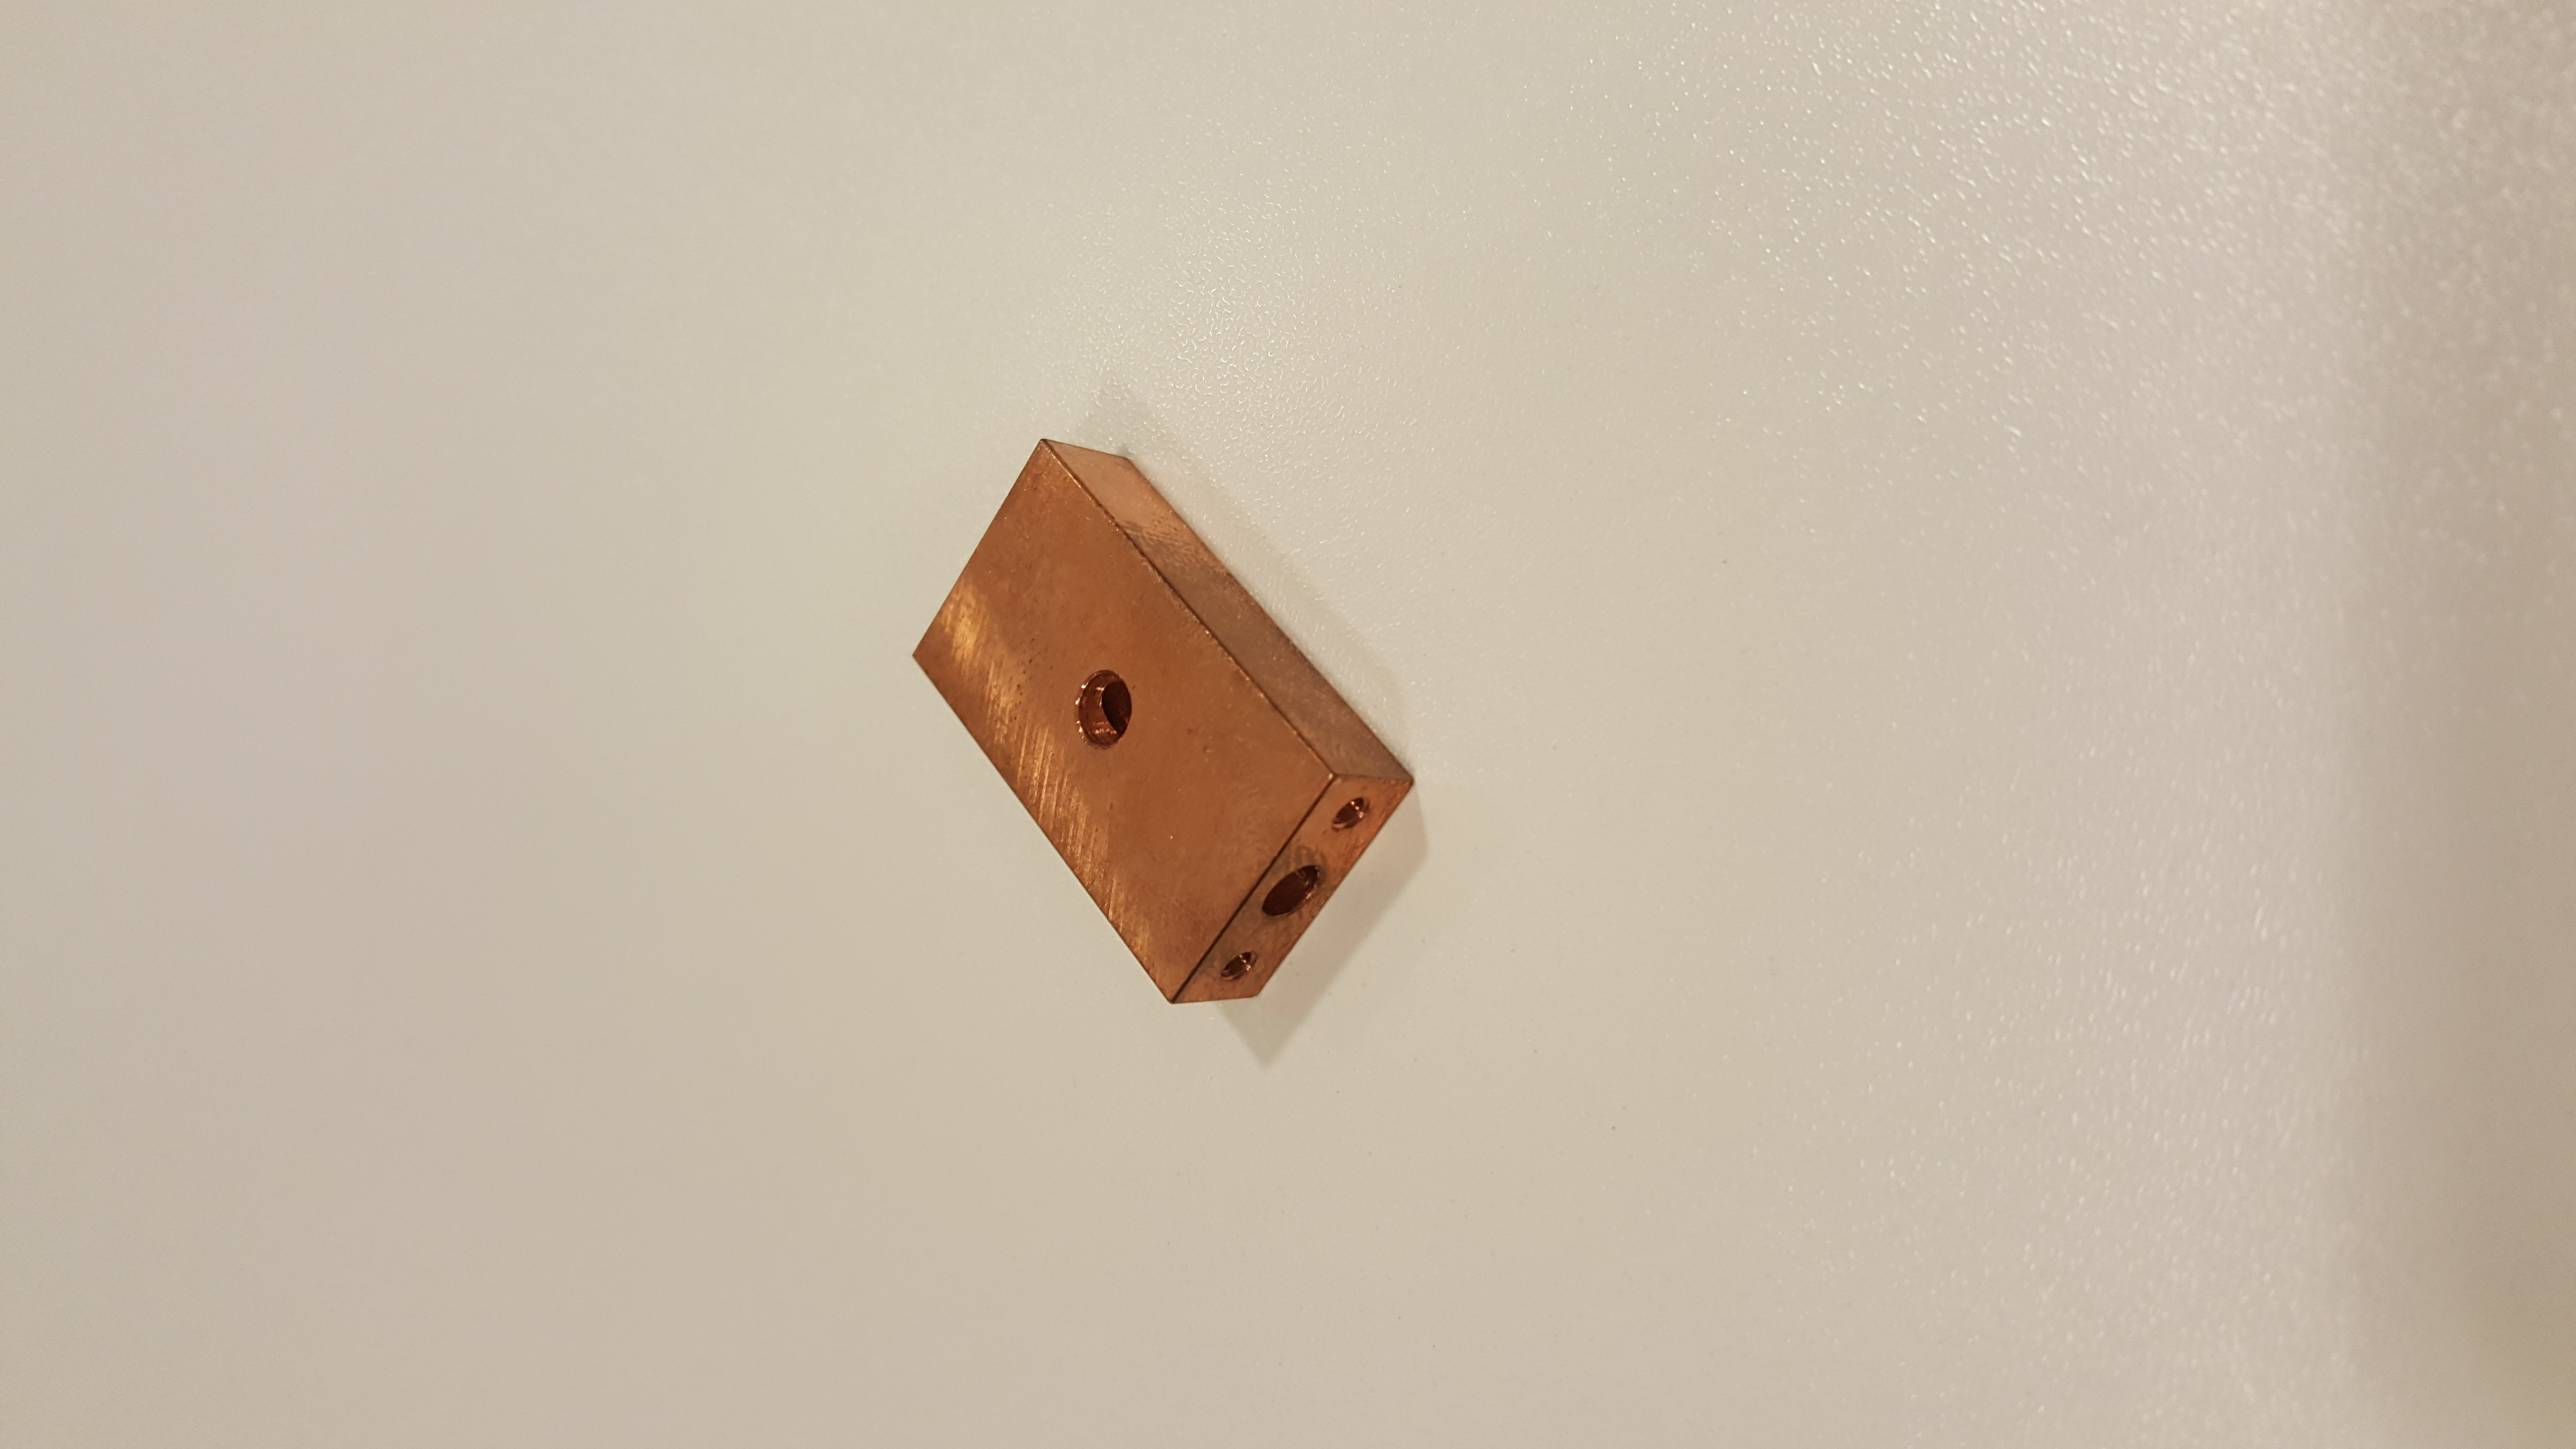
\includegraphics[angle=-90,trim=1550 300 1950 300,clip,width=0.975\linewidth]{figure/Filterbilder/filterbox.jpg}
    \caption{Maskinarbetat kopparblock för att konstruera att distribuerat lågpassfilter.}
    \label{fig:filterbox}
\end{wrapfigure}
I detta projekt har vi konstruerat ett distribuerat lågpassfilter genom att i en koaxial geometri ersätta en del av det isolerande dielektrikum mellan centerledare och hölje med ett dielektrikum med frekvensberoende förluster för att på så sätt effektivt dämpa höga frekvenser.  

De distribuerade lågpassfilter som konstruerats i detta projekt består i huvudsak av tre olika delar: två cylindriska SMA kontakter med en delvis isolerad centerledare, Emerson \& Cuming Stycast 1266 och ett rektangulärt block av maskinarbetad koppar som visas i figur \ref{fig:filterbox}. Från kopparblockets kortsida har ett hål borrats genom hela blocket för att ge plats åt de två SMA kontakterna som ska föras in i kopparblockat från var sin sida och agera som filtrets centerledare. På de båda kortsidorna finns också två skruvhål borrade för att kunna fästa SMA kontakten vid kopparblocket. Från kopparblockets ovansida har ett titthål borrats för att kunna löda ihop de två SMA kontakterna samt för att kunna fylla hålrummet mellan den oisolerade centerledaren och kopparblocket med Stycast som är ett dielektrikum med förluster för att ge filtret en frekvensberoende dämpning som diskuteras i avsnitt \ref{sec:filterdesign}.

\begin{comment}
Om det här blir bra:
- Så här har vi bestämt att göra filtrena - introducera hur de ser ut osv så att man får ett hum om dem
- Varför vi har gjort det (teoriförklaring) - varför valde vi denna metod osv
- Konstruktion av filter - hur vi konstruerade och varför vi gjorde på det sättet
- Mätningar och filterkarakteristik
\end{comment}

\section{Filterdesign}
\label{sec:filterdesign}
För att undersöka egenskaperna hos en transmissionsledning kan man utgå från propagationskonstanten $\gamma =\sqrt{(R+j\omega L)+(G+j\omega C)} $ för en generell transmissionsledning\autocite{cheng}. Där $R$ är resistans per längdenhet, $L$ induktans per längdenhet, $G$ konduktans per längdenhet och $C$ kapacitans per längdenhet.

För en koaxial geometri som vårt distribuerade filter är baserad på ges $R, L, G$ och $C$ av
\begin{equation*}
    R=\frac{1}{2\pi}\sqrt{\frac{\pi f\mu_c}{\sigma_c}}\left(\frac{1}{a}+\frac{1}{b}\right),\hspace{1em} L=\frac{\mu}{2\pi}\ln\frac{b}{a},\hspace{1em}G=\frac{2\pi\sigma}{\ln\frac{b}{a}},\hspace{1em}C=\frac{2\pi\epsilon}{\ln\frac{b}{a}}
\end{equation*}
Där $a$ och $b$ är inner- respektive ytterradie, $\mu_c=\mu_r\mu_0$ är ledarens permeabilitet, $\sigma_c$ ledarens konduktivitet, $\sigma$ är dielektrikumets konduktivitet och $\epsilon =\epsilon_r\epsilon_0$ är dielektrikumets permittivitet. 
 

Genom att välja $a=\unit[0,64]{mm}$ och $b=\unit[2,03]{mm}$, vilket motsvarar dimensionerna på vårt filter som konstruerats i detta projekt. Vidare antar vi att ledaren består av koppar vilket ger $\mu_c=\mu_0$ och $\sigma_c=\unit[5,96\cdot 10^7]{S/m}$. Om vi också antar att vårt dielektrikum har $\epsilon=3\epsilon_0$ och en dielektrisk förlusttangent $\delta_e$ som kan relateras till dielektrikumets konduktivitet genom
\begin{equation*}
    \tan\delta_e=\frac{\epsilon^{''}}{\epsilon'}\approx\frac{\sigma}{\omega\epsilon}
\end{equation*}
\autocite{cheng}. Så kan dämpningen som funktion av frekvens och förlusttangent beräknas, vilket visas i \figref{fig:attn_ex}.

\begin{figure}[H]
    
        \centering
        \setlength\figurewidth{0.75\linewidth}
        \setlength\figureheight{12em}
        % This file was created by matlab2tikz.
%
\definecolor{mycolor1}{rgb}{0.20810,0.16630,0.52920}%
\definecolor{mycolor2}{rgb}{0.21162,0.18978,0.57768}%
\definecolor{mycolor3}{rgb}{0.20810,0.23860,0.67709}%
\definecolor{mycolor4}{rgb}{0.19590,0.26446,0.72790}%
\definecolor{mycolor5}{rgb}{0.12527,0.32424,0.83027}%
\definecolor{mycolor6}{rgb}{0.01170,0.38751,0.88196}%
\definecolor{mycolor7}{rgb}{0.00596,0.40861,0.88284}%
\definecolor{mycolor8}{rgb}{0.03285,0.44304,0.87196}%
\definecolor{mycolor9}{rgb}{0.04981,0.45857,0.86406}%
\definecolor{mycolor10}{rgb}{0.07227,0.48867,0.84670}%
\definecolor{mycolor11}{rgb}{0.07935,0.52002,0.83118}%
\definecolor{mycolor12}{rgb}{0.07494,0.53754,0.82627}%
\definecolor{mycolor13}{rgb}{0.04877,0.57722,0.82283}%
\definecolor{mycolor14}{rgb}{0.03434,0.59658,0.81985}%
\definecolor{mycolor15}{rgb}{0.02389,0.62866,0.80376}%
\definecolor{mycolor16}{rgb}{0.02277,0.65349,0.77676}%
\definecolor{mycolor17}{rgb}{0.02666,0.66420,0.76072}%
\definecolor{mycolor18}{rgb}{0.05897,0.68376,0.72539}%
\definecolor{mycolor19}{rgb}{0.08430,0.69283,0.70617}%
\definecolor{mycolor20}{rgb}{0.14527,0.70976,0.66463}%
\definecolor{mycolor21}{rgb}{0.21783,0.72504,0.61926}%
\definecolor{mycolor22}{rgb}{0.25864,0.73171,0.59543}%
\definecolor{mycolor23}{rgb}{0.34817,0.74243,0.54727}%
\definecolor{mycolor24}{rgb}{0.39526,0.74590,0.52444}%
\definecolor{mycolor25}{rgb}{0.48712,0.74906,0.48398}%
\definecolor{mycolor26}{rgb}{0.57086,0.74852,0.44939}%
\definecolor{mycolor27}{rgb}{0.60985,0.74731,0.43369}%
\definecolor{mycolor28}{rgb}{0.68342,0.74348,0.40443}%
\definecolor{mycolor29}{rgb}{0.71841,0.74113,0.39048}%
\definecolor{mycolor30}{rgb}{0.78584,0.73557,0.36327}%
\definecolor{mycolor31}{rgb}{0.85066,0.72990,0.33603}%
\definecolor{mycolor32}{rgb}{0.88243,0.72743,0.32170}%
\definecolor{mycolor33}{rgb}{0.94496,0.72611,0.28864}%
\definecolor{mycolor34}{rgb}{0.97390,0.73140,0.26665}%
\definecolor{mycolor35}{rgb}{0.99904,0.76531,0.21641}%
\definecolor{mycolor36}{rgb}{0.98800,0.80660,0.17937}%
\definecolor{mycolor37}{rgb}{0.97886,0.82714,0.16331}%
\definecolor{mycolor38}{rgb}{0.96259,0.87051,0.13090}%
\definecolor{mycolor39}{rgb}{0.95887,0.89490,0.11324}%
\definecolor{mycolor40}{rgb}{0.96610,0.95144,0.07553}%
\definecolor{mycolor41}{rgb}{0.97630,0.98310,0.05380}%
%
\begin{tikzpicture}[%
trim axis left, trim axis right
]

\begin{axis}[%
width=0.893\figurewidth,
height=\figureheight,
at={(0\figurewidth,0\figureheight)},
scale only axis,
point meta min=0,
point meta max=9.26148497339275,
xmin=0,
xmax=100,
xlabel style={font=\color{white!15!black}},
xlabel={Frekvens (\unit{GHz})},
ymin=0,
ymax=0.06,
ylabel style={font=\color{white!15!black}},
y tick label style={/pgf/number format/.cd, fixed, precision=2},
scaled y ticks = false,
ylabel={Förlusttangent $\delta_e$},
axis background/.style={fill=white},
title style={font=\bfseries},
title={Dämpning som funktion av frekvens och $\delta_e$ (\unit{dB/cm})},
colormap={mymap}{[1pt] rgb(0pt)=(0.2081,0.1663,0.5292); rgb(1pt)=(0.211624,0.189781,0.577676); rgb(2pt)=(0.212252,0.213771,0.626971); rgb(3pt)=(0.2081,0.2386,0.677086); rgb(4pt)=(0.195905,0.264457,0.7279); rgb(5pt)=(0.170729,0.291938,0.779248); rgb(6pt)=(0.125271,0.324243,0.830271); rgb(7pt)=(0.0591333,0.359833,0.868333); rgb(8pt)=(0.0116952,0.38751,0.881957); rgb(9pt)=(0.00595714,0.408614,0.882843); rgb(10pt)=(0.0165143,0.4266,0.878633); rgb(11pt)=(0.0328524,0.443043,0.871957); rgb(12pt)=(0.0498143,0.458571,0.864057); rgb(13pt)=(0.0629333,0.47369,0.855438); rgb(14pt)=(0.0722667,0.488667,0.8467); rgb(15pt)=(0.0779429,0.503986,0.838371); rgb(16pt)=(0.0793476,0.520024,0.831181); rgb(17pt)=(0.0749429,0.537543,0.826271); rgb(18pt)=(0.0640571,0.556986,0.823957); rgb(19pt)=(0.0487714,0.577224,0.822829); rgb(20pt)=(0.0343429,0.596581,0.819852); rgb(21pt)=(0.0265,0.6137,0.8135); rgb(22pt)=(0.0238905,0.628662,0.803762); rgb(23pt)=(0.0230905,0.641786,0.791267); rgb(24pt)=(0.0227714,0.653486,0.776757); rgb(25pt)=(0.0266619,0.664195,0.760719); rgb(26pt)=(0.0383714,0.674271,0.743552); rgb(27pt)=(0.0589714,0.683757,0.725386); rgb(28pt)=(0.0843,0.692833,0.706167); rgb(29pt)=(0.113295,0.7015,0.685857); rgb(30pt)=(0.145271,0.709757,0.664629); rgb(31pt)=(0.180133,0.717657,0.642433); rgb(32pt)=(0.217829,0.725043,0.619262); rgb(33pt)=(0.258643,0.731714,0.595429); rgb(34pt)=(0.302171,0.737605,0.571186); rgb(35pt)=(0.348167,0.742433,0.547267); rgb(36pt)=(0.395257,0.7459,0.524443); rgb(37pt)=(0.44201,0.748081,0.503314); rgb(38pt)=(0.487124,0.749062,0.483976); rgb(39pt)=(0.530029,0.749114,0.466114); rgb(40pt)=(0.570857,0.748519,0.44939); rgb(41pt)=(0.609852,0.747314,0.433686); rgb(42pt)=(0.6473,0.7456,0.4188); rgb(43pt)=(0.683419,0.743476,0.404433); rgb(44pt)=(0.71841,0.741133,0.390476); rgb(45pt)=(0.752486,0.7384,0.376814); rgb(46pt)=(0.785843,0.735567,0.363271); rgb(47pt)=(0.818505,0.732733,0.34979); rgb(48pt)=(0.850657,0.7299,0.336029); rgb(49pt)=(0.882433,0.727433,0.3217); rgb(50pt)=(0.913933,0.725786,0.306276); rgb(51pt)=(0.944957,0.726114,0.288643); rgb(52pt)=(0.973895,0.731395,0.266648); rgb(53pt)=(0.993771,0.745457,0.240348); rgb(54pt)=(0.999043,0.765314,0.216414); rgb(55pt)=(0.995533,0.786057,0.196652); rgb(56pt)=(0.988,0.8066,0.179367); rgb(57pt)=(0.978857,0.827143,0.163314); rgb(58pt)=(0.9697,0.848138,0.147452); rgb(59pt)=(0.962586,0.870514,0.1309); rgb(60pt)=(0.958871,0.8949,0.113243); rgb(61pt)=(0.959824,0.921833,0.0948381); rgb(62pt)=(0.9661,0.951443,0.0755333); rgb(63pt)=(0.9763,0.9831,0.0538)},
colorbar,
colorbar style={ylabel style={font=\color{white!15!black}}, ylabel={Dämpning (\unit{dB/cm})}}
]
\addplot[fill=mycolor1, draw=none, forget plot] table[row sep=crcr] {%
%
x	y\\
0	0\\
0	0.06\\
100	0.06\\
100	0\\
};
\addplot[fill=mycolor2, draw=none, forget plot] table[row sep=crcr] {%
%
x	y\\
2.39916877208826	0.06\\
2.41118122323781	0.0596984924623116\\
2.42331429363386	0.0593969849246231\\
2.43556981059405	0.0590954773869347\\
2.44794963853383	0.0587939698492462\\
2.4604556799127	0.0584924623115578\\
2.47308987620957	0.0581909547738693\\
2.48585420892828	0.0578894472361809\\
2.49875070063437	0.0575879396984925\\
2.51178141602424	0.057286432160804\\
2.51256281407035	0.0572684510017686\\
2.52496107982541	0.0569849246231156\\
2.53828030252747	0.0566834170854271\\
2.55174049690882	0.0563819095477387\\
2.56534391452555	0.0560804020100503\\
2.57909285513858	0.0557788944723618\\
2.59298966801062	0.0554773869346734\\
2.60703675324525	0.0551758793969849\\
2.62123656316976	0.0548743718592965\\
2.63559160376334	0.054572864321608\\
2.65010443613235	0.0542713567839196\\
2.6647776780346	0.0539698492462312\\
2.67961400545449	0.0536683417085427\\
2.69461615423096	0.0533668341708543\\
2.70978692174034	0.0530653266331658\\
2.72512916863641	0.0527638190954774\\
2.74064582064972	0.0524623115577889\\
2.75633987044873	0.0521608040201005\\
2.77221437956517	0.0518592964824121\\
2.78827248038619	0.0515577889447236\\
2.80451737821619	0.0512562814070352\\
2.82095235341094	0.0509547738693467\\
2.83758076358718	0.0506532663316583\\
2.85440604591069	0.0503517587939698\\
2.87143171946621	0.0500502512562814\\
2.88866138771255	0.049748743718593\\
2.90609874102655	0.0494472361809045\\
2.92374755933964	0.0491457286432161\\
2.94161171487094	0.0488442211055276\\
2.95969517496109	0.0485427135678392\\
2.97800200501116	0.0482412060301508\\
2.99653637153113	0.0479396984924623\\
3.01507537688442	0.0476418183242245\\
3.01530275487233	0.0476381909547739\\
3.03432275629165	0.0473366834170854\\
3.05358388129042	0.047035175879397\\
3.07309074658588	0.0467336683417085\\
3.09284808751206	0.0464321608040201\\
3.11286076185384	0.0461306532663317\\
3.13313375383082	0.0458291457286432\\
3.15367217823771	0.0455276381909548\\
3.17448128474842	0.0452261306532663\\
3.19556646239164	0.0449246231155779\\
3.21693324420576	0.0446231155778894\\
3.23858731208164	0.044321608040201\\
3.26053450180211	0.0440201005025126\\
3.28278080828767	0.0437185929648241\\
3.30533239105816	0.0434170854271357\\
3.32819557992092	0.0431155778894472\\
3.3513768808966	0.0428140703517588\\
3.37488298239394	0.0425125628140704\\
3.39872076164626	0.0422110552763819\\
3.4228972914223	0.0419095477386935\\
3.44741984702537	0.041608040201005\\
3.47229591359532	0.0413065326633166\\
3.49753319372869	0.0410050251256281\\
3.51758793969849	0.0407685141320628\\
3.52314435677785	0.0407035175879397\\
3.54915047159738	0.0404020100502513\\
3.57554296099497	0.0401005025125628\\
3.60233050309453	0.0397989949748744\\
3.62952203786567	0.0394974874371859\\
3.65712677707465	0.0391959798994975\\
3.68515421469257	0.038894472361809\\
3.71361413778555	0.0385929648241206\\
3.74251663791315	0.0382914572864322\\
3.77187212306285	0.0379899497487437\\
3.80169133015032	0.0376884422110553\\
3.83198533811699	0.0373869346733668\\
3.86276558165847	0.0370854271356784\\
3.89404386561956	0.0367839195979899\\
3.92583238009392	0.0364824120603015\\
3.95814371626907	0.0361809045226131\\
3.99099088305973	0.0358793969849246\\
4.02010050251256	0.0356163112090361\\
4.02439074485247	0.0355778894472362\\
4.05837771133621	0.0352763819095477\\
4.09294315511978	0.0349748743718593\\
4.12810197604806	0.0346733668341709\\
4.16386959009777	0.0343718592964824\\
4.20026195192127	0.034070351758794\\
4.23729557858233	0.0337688442211055\\
4.27498757455822	0.0334673366834171\\
4.31335565808741	0.0331658291457286\\
4.35241818894835	0.0328643216080402\\
4.3921941977607	0.0325628140703518\\
4.43270341690731	0.0322613065326633\\
4.47396631318255	0.0319597989949749\\
4.51600412228035	0.0316582914572864\\
4.52261306532663	0.0316113994725947\\
4.55886631568272	0.031356783919598\\
4.60255455251199	0.0310552763819095\\
4.64708769962313	0.0307537688442211\\
4.69249051185516	0.0304522613065327\\
4.73878872063326	0.0301507537688442\\
4.78600908260686	0.0298492462311558\\
4.83417943122368	0.0295477386934673\\
4.88332873144875	0.0292462311557789\\
4.93348713785456	0.0289447236180905\\
4.98468605632686	0.028643216080402\\
5.0251256281407	0.0284094100262554\\
5.03696666143708	0.0283417085427136\\
5.09038478089173	0.0280402010050251\\
5.1449474766273	0.0277386934673367\\
5.20069194029564	0.0274371859296482\\
5.257656992524	0.0271356783919598\\
5.31588317308776	0.0268341708542714\\
5.37541283714012	0.0265326633165829\\
5.43629025797872	0.0262311557788945\\
5.49856173687321	0.025929648241206\\
5.52763819095477	0.0257911903368306\\
5.56229940490022	0.0256281407035176\\
5.62755199918398	0.0253266331658291\\
5.69435309958229	0.0250251256281407\\
5.76275849721406	0.0247236180904523\\
5.83282669590745	0.0244221105527638\\
5.90461907910231	0.0241206030150754\\
5.9782000892289	0.0238190954773869\\
6.03015075376884	0.0236106506144935\\
6.05365276377166	0.0235175879396985\\
6.13106895302203	0.0232160804020101\\
6.2104901282578	0.0229145728643216\\
6.29199521089676	0.0226130653266332\\
6.37566731949395	0.0223115577889447\\
6.46159405251227	0.0220100502512563\\
6.53266331658291	0.0217666669865902\\
6.54987858206708	0.0217085427135678\\
6.64065465531511	0.0214070351758794\\
6.73398148414327	0.021105527638191\\
6.82996812391891	0.0208040201005025\\
6.92872993664582	0.0205025125628141\\
7.03038905354026	0.0202010050251256\\
7.03517587939699	0.020187022632728\\
7.13513595780296	0.0198994974874372\\
7.24305357966992	0.0195979899497487\\
7.35428495667874	0.0192964824120603\\
7.46898511203338	0.0189949748743719\\
7.53768844221106	0.0188187702198402\\
7.58734799773952	0.0186934673366834\\
7.70956411496069	0.018391959798995\\
7.8357810755178	0.0180904522613065\\
7.96619861998384	0.0177889447236181\\
8.04020100502513	0.0176222099403199\\
8.1010645976823	0.0174874371859296\\
8.24061904658568	0.0171859296482412\\
8.38506492859059	0.0168844221105528\\
8.53466401823787	0.0165829145728643\\
8.5427135678392	0.0165669905007729\\
8.68977899809873	0.0162814070351759\\
8.85064040302216	0.0159798994974874\\
9.01756868684697	0.015678391959799\\
9.04522613065327	0.0156295111772917\\
9.1909925123221	0.0153768844221106\\
9.3712324082404	0.0150753768844221\\
9.54773869346734	0.0147911456407552\\
9.55868747061573	0.0147738693467337\\
9.75389121239623	0.0144723618090452\\
9.95723276134825	0.0141708542713568\\
10.0502512562814	0.0140369961592338\\
10.1692927263288	0.0138693467336683\\
10.3906312947426	0.0135678391959799\\
10.5527638190955	0.0133550066657412\\
10.6218523577211	0.0132663316582915\\
10.8636831603175	0.012964824120603\\
11.0552763819095	0.0127353152321263\\
11.1168107253371	0.0126633165829146\\
11.3821140064104	0.0123618090452261\\
11.5577889447236	0.0121697773699802\\
11.6604373427429	0.0120603015075377\\
11.9528020449368	0.0117587939698492\\
12.0603015075377	0.0116516079467992\\
12.2602973748408	0.0114572864321608\\
12.5628140703518	0.0111751089508643\\
12.5840943742805	0.0111557788944724\\
12.9256056090151	0.0108542713567839\\
13.0653266331658	0.0107354598675858\\
13.2862682859805	0.0105527638190955\\
13.5678391959799	0.0103285560388275\\
13.667746817269	0.010251256281407\\
14.070351758794	0.00995087971360513\\
14.0719131310119	0.00994974874371859\\
14.5008978939826	0.00964824120603015\\
14.572864321608	0.00959939890897161\\
14.9570247733361	0.00934673366834171\\
15.0753768844221	0.00927148702130651\\
15.4429670176522	0.00904522613065327\\
15.5778894472362	0.00896485670504451\\
15.9617593017348	0.00874371859296482\\
16.0804020100503	0.00867750703444799\\
16.5168604285404	0.00844221105527638\\
16.5829145728643	0.00840768005618042\\
17.0854271356784	0.00815382497196046\\
17.1122409355137	0.00814070351758794\\
17.5879396984925	0.00791456847916677\\
17.7524891280069	0.0078391959798995\\
18.0904522613065	0.00768869036251839\\
18.4428495143081	0.00753768844221106\\
18.5929648241206	0.00747510247439751\\
19.0954773869347	0.00727283132914252\\
19.1894858768464	0.00723618090452261\\
19.5979899497487	0.00708100348801239\\
19.9996126205682	0.00693467336683417\\
20.1005025125628	0.00689883328951856\\
20.6030150753769	0.00672561147912859\\
20.881720070714	0.00663316582914573\\
21.105527638191	0.00656069684668912\\
21.608040201005	0.00640350774194304\\
21.8458732281893	0.00633165829145729\\
22.1105527638191	0.00625351557887704\\
22.6130653266332	0.00611023885084019\\
22.9041379318985	0.00603015075376884\\
23.1155778894472	0.0059732380275962\\
23.6180904522613	0.00584211099156639\\
24.0710529103974	0.0057286432160804\\
24.1206030150754	0.00571648940500242\\
24.6231155778894	0.0055960347130659\\
25.1256281407035	0.00548043594968593\\
25.3643789052266	0.00542713567839196\\
25.6281407035176	0.00536940624772572\\
26.1306532663317	0.00526268098820719\\
26.6331658291457	0.00516001566498357\\
26.8058849514255	0.00512562814070352\\
27.1356783919598	0.00506118369932857\\
27.6381909547739	0.00496597521473994\\
28.1407035175879	0.00487419536906242\\
28.4227416203296	0.00482412060301507\\
28.643216080402	0.00478566289426998\\
29.1457286432161	0.00470020910575334\\
29.6482412060302	0.00461767689129826\\
30.1507537688442	0.00453791955388712\\
30.2491764101157	0.00452261306532663\\
30.6532663316583	0.00446079993431147\\
31.1557788944724	0.00438618993056607\\
31.6582914572864	0.00431396954269985\\
32.1608040201005	0.00424402626615832\\
32.3290168791508	0.00422110552763819\\
32.6633165829146	0.00417625446613082\\
33.1658291457286	0.00411055503429614\\
33.6683417085427	0.00404683479601743\\
34.1708542713568	0.0039850060379632\\
34.6733668341709	0.00392498614592814\\
34.71921543835	0.00391959798994975\\
35.1758793969849	0.00386669716051632\\
35.678391959799	0.00381006567565387\\
36.1809045226131	0.00375502231341366\\
36.6834170854271	0.00370150150078516\\
37.1859296482412	0.00364944121960533\\
37.4953238130822	0.00361809045226131\\
37.6884422110553	0.00359878274232376\\
38.1909547738694	0.00354947045201629\\
38.6934673366834	0.00350145168701522\\
39.1959798994975	0.00345467645315278\\
39.6984924623116	0.00340909729528336\\
40.2010050251256	0.00336466913826008\\
40.7035175879397	0.00332134913970931\\
40.7595884451542	0.00331658291457286\\
41.2060301507538	0.00327909650593007\\
41.7085427135678	0.00323787250358902\\
42.2110552763819	0.00319764021472093\\
42.713567839196	0.00315836445838398\\
43.2160804020101	0.00312001169515612\\
43.7185929648241	0.00308254993258642\\
44.2211055276382	0.00304594863710345\\
44.6541530746058	0.00301507537688442\\
44.7236180904523	0.00301017864620675\\
45.2261306532663	0.00297521207401917\\
45.7286432160804	0.0029410223279625\\
46.2311557788945	0.0029075839413017\\
46.7336683417085	0.00287487254627658\\
47.2361809045226	0.0028428648155108\\
47.7386934673367	0.00281153840712777\\
48.2412060301508	0.00278087191330272\\
48.7437185929648	0.00275084481200272\\
49.2462311557789	0.00272143742168647\\
49.3825004891009	0.00271356783919598\\
49.748743718593	0.00269263083693153\\
50.251256281407	0.00266440694632044\\
50.7537688442211	0.00263674835272531\\
51.2562814070352	0.00260963833575687\\
51.7587939698492	0.00258306082663756\\
52.2613065326633	0.00255700037679765\\
52.7638190954774	0.00253144212826909\\
53.2663316582915	0.00250637178575826\\
53.7688442211055	0.00248177559028763\\
54.2713567839196	0.00245764029430448\\
54.7738693467337	0.0024339531381623\\
55.2467687898493	0.00241206030150754\\
55.2763819095477	0.00241070182662722\\
55.7788944723618	0.00238787449171531\\
56.2814070351759	0.00236545972914004\\
56.78391959799	0.00234344652020499\\
57.286432160804	0.00232182423426683\\
57.7889447236181	0.00230058261181994\\
58.2914572864322	0.00227971174845765\\
58.7939698492462	0.0022592020796576\\
59.2964824120603	0.0022390443663422\\
59.7989949748744	0.00221922968116857\\
60.3015075376884	0.00219974939550531\\
60.8040201005025	0.00218059516705634\\
61.3065326633166	0.00216175892809461\\
61.8090452261307	0.00214323287427088\\
62.3115577889447	0.00212500945396516\\
62.7161374052462	0.0021105527638191\\
62.8140703517588	0.00210708135532836\\
63.3165829145729	0.00208944149357922\\
63.8190954773869	0.00207208302812174\\
64.321608040201	0.00205499932158766\\
64.8241206030151	0.00203818394323375\\
65.3266331658292	0.00202163066097276\\
65.8291457286432	0.00200533343377017\\
66.3316582914573	0.00198928640438721\\
66.8341708542714	0.00197348389245197\\
67.3366834170854	0.00195792038784141\\
67.8391959798995	0.00194259054435809\\
68.3417085427136	0.00192748917368647\\
68.8442211055276	0.00191261123961447\\
69.3467336683417	0.00189795185250677\\
69.8492462311558	0.00188350626401719\\
70.3517587939699	0.0018692698620282\\
70.8542713567839	0.00185523816580617\\
71.356783919598	0.00184140682136179\\
71.8592964824121	0.00182777159700564\\
72.3618090452261	0.00181432837908921\\
72.5612633284531	0.00180904522613065\\
72.8643216080402	0.00180107316235816\\
73.3668341708543	0.00178800205917377\\
73.8693467336683	0.00177511128986651\\
74.3718592964824	0.00176239717376795\\
74.8743718592965	0.00174985612944251\\
75.3768844221106	0.00173748467136988\\
75.8793969849246	0.00172527940675953\\
76.3819095477387	0.00171323703249118\\
76.8844221105528	0.00170135433217566\\
77.3869346733668	0.00168962817333037\\
77.8894472361809	0.0016780555046645\\
78.391959798995	0.00166663335346871\\
78.8944723618091	0.00165535882310499\\
79.3969849246231	0.00164422909059189\\
79.8994974874372	0.00163324140428121\\
80.4020100502512	0.00162239308162193\\
80.9045226130653	0.00161168150700769\\
81.4070351758794	0.00160110412970419\\
81.9095477386935	0.00159065846185307\\
82.4120603015075	0.00158034207654892\\
82.9145728643216	0.00157015260598648\\
83.4170854271357	0.00156008773967487\\
83.9195979899498	0.0015501452227162\\
84.4221105527638	0.00154032285414578\\
84.9246231155779	0.00153061848533137\\
85.427135678392	0.0015210300184291\\
85.929648241206	0.00151155540489369\\
86.1445672354202	0.00150753768844221\\
86.4321608040201	0.00150219264092433\\
86.9346733668342	0.00149293977314838\\
87.4371859296483	0.00148379489482959\\
87.9396984924623	0.00147475614072878\\
88.4422110552764	0.00146582168819702\\
88.9447236180905	0.0014569897559686\\
89.4472361809045	0.0014482586029948\\
89.9497487437186	0.00143962652731681\\
90.4522613065327	0.00143109186497634\\
90.9547738693468	0.00142265298896242\\
91.4572864321608	0.00141430830819301\\
91.9597989949749	0.00140605626653005\\
92.462311557789	0.00139789534182681\\
92.964824120603	0.00138982404500604\\
93.4673366834171	0.00138184091916814\\
93.9698492462312	0.00137394453872781\\
94.4723618090452	0.00136613350857848\\
94.9748743718593	0.00135840646328328\\
95.4773869346734	0.00135076206629156\\
95.9798994974875	0.00134319900918019\\
96.4824120603015	0.00133571601091858\\
96.9849246231156	0.00132831181715656\\
97.4874371859297	0.00132098519953445\\
97.9899497487437	0.0013137349550143\\
98.4924623115578	0.00130655990523173\\
98.9949748743719	0.00129945889586753\\
99.4974874371859	0.00129243079603837\\
100	0.00128547449770589\\
100	0.06\\
};
\addplot[fill=mycolor3, draw=none, forget plot] table[row sep=crcr] {%
%
x	y\\
4.82581546407028	0.06\\
4.85005457243024	0.0596984924623116\\
4.87453784891348	0.0593969849246231\\
4.89926900441046	0.0590954773869347\\
4.92425182539241	0.0587939698492462\\
4.94949017584535	0.0584924623115578\\
4.97498799926392	0.0581909547738693\\
5.00074932070694	0.0578894472361809\\
5.0251256281407	0.0576069900621348\\
5.02677883387327	0.0575879396984925\\
5.05308892452473	0.057286432160804\\
5.07967529646647	0.0569849246231156\\
5.10654232758541	0.0566834170854271\\
5.13369448875413	0.0563819095477387\\
5.16113634631275	0.0560804020100503\\
5.18887256463081	0.0557788944723618\\
5.21690790875208	0.0554773869346734\\
5.24524724712539	0.0551758793969849\\
5.27389555442497	0.0548743718592965\\
5.30285791446344	0.054572864321608\\
5.33213952320134	0.0542713567839196\\
5.3617456918567	0.0539698492462312\\
5.3916818501187	0.0536683417085427\\
5.4219535494694	0.0533668341708543\\
5.45256646661799	0.0530653266331658\\
5.48352640705171	0.0527638190954774\\
5.51483930870848	0.0524623115577889\\
5.52763819095477	0.0523400539557542\\
5.54651763297627	0.0521608040201005\\
5.57856576163893	0.0518592964824121\\
5.61098575300923	0.0515577889447236\\
5.64378412085523	0.0512562814070352\\
5.67696753197042	0.0509547738693467\\
5.71054281069397	0.0506532663316583\\
5.74451694359218	0.0503517587939698\\
5.77889708430781	0.0500502512562814\\
5.81369055858451	0.049748743718593\\
5.84890486947354	0.0494472361809045\\
5.88454770273075	0.0491457286432161\\
5.92062693241185	0.0488442211055276\\
5.95715062667465	0.0485427135678392\\
5.99412705379707	0.0482412060301508\\
6.03015075376884	0.0479510177227778\\
6.03156514504727	0.0479396984924623\\
6.06948499658896	0.0476381909547739\\
6.10788396256955	0.0473366834170854\\
6.14677118555362	0.047035175879397\\
6.18615604220853	0.0467336683417085\\
6.22604815084569	0.0464321608040201\\
6.26645737925524	0.0461306532663317\\
6.30739385284751	0.0458291457286432\\
6.34886796311545	0.0455276381909548\\
6.3908903764328	0.0452261306532663\\
6.43347204320373	0.0449246231155779\\
6.4766242073803	0.0446231155778894\\
6.5203584163653	0.044321608040201\\
6.53266331658291	0.0442375032531293\\
6.56469651321973	0.0440201005025126\\
6.60964489031862	0.0437185929648241\\
6.65521227111241	0.0434170854271357\\
6.70141153643031	0.0431155778894472\\
6.74825592697998	0.0428140703517588\\
6.79575905600432	0.0425125628140704\\
6.84393492247617	0.0422110552763819\\
6.89279792485773	0.0419095477386935\\
6.94236287545337	0.041608040201005\\
6.99264501538553	0.0413065326633166\\
7.03517587939699	0.0410548647854148\\
7.04366256925818	0.0410050251256281\\
7.09544222914052	0.0407035175879397\\
7.14798799825932	0.0404020100502513\\
7.20131701200114	0.0401005025125628\\
7.25544692060852	0.0397989949748744\\
7.31039590866329	0.0394974874371859\\
7.36618271546137	0.0391959798994975\\
7.42282665632698	0.038894472361809\\
7.48034764491725	0.0385929648241206\\
7.53768844221106	0.0382969775358106\\
7.53876652786388	0.0382914572864322\\
7.59812113973274	0.0379899497487437\\
7.65841691943149	0.0376884422110553\\
7.7196764386326	0.0373869346733668\\
7.78192299659539	0.0370854271356784\\
7.84518064972095	0.0367839195979899\\
7.90947424255953	0.0364824120603015\\
7.97482944035433	0.0361809045226131\\
8.04020100502513	0.0358842208832709\\
8.04127306295999	0.0358793969849246\\
8.10885097782135	0.0355778894472362\\
8.17757341616917	0.0352763819095477\\
8.24746971046934	0.0349748743718593\\
8.31857020415516	0.0346733668341709\\
8.39090629556067	0.0343718592964824\\
8.4645104841651	0.034070351758794\\
8.53941641929148	0.0337688442211055\\
8.5427135678392	0.0337556940313074\\
8.61567891219899	0.0334673366834171\\
8.69331575680882	0.0331658291457286\\
8.77236350783384	0.0328643216080402\\
8.85286098817671	0.0325628140703518\\
8.93484845827451	0.0322613065326633\\
9.01836768325667	0.0319597989949749\\
9.04522613065327	0.0318640210199441\\
9.10347746036427	0.0316582914572864\\
9.19021524956768	0.031356783919598\\
9.27862074794658	0.0310552763819095\\
9.36874253039696	0.0307537688442211\\
9.46063107674587	0.0304522613065327\\
9.54773869346734	0.0301717962702774\\
9.55434056160362	0.0301507537688442\\
9.64994698912681	0.0298492462311558\\
9.74748502891313	0.0295477386934673\\
9.8470138286839	0.0292462311557789\\
9.94859497593889	0.0289447236180905\\
10.0502512562814	0.0286490914551562\\
10.0522931360319	0.028643216080402\\
10.1582009306533	0.0283417085427136\\
10.2663629320562	0.0280402010050251\\
10.3768518970681	0.0277386934673367\\
10.4897437476362	0.0274371859296482\\
10.5527638190955	0.0272716781554462\\
10.6051305964441	0.0271356783919598\\
10.7230989421272	0.0268341708542714\\
10.8437200561137	0.0265326633165829\\
10.9670844498629	0.0262311557788945\\
11.0552763819095	0.0260197337563562\\
11.0932959036347	0.025929648241206\\
11.222466689639	0.0256281407035176\\
11.3546797513822	0.0253266331658291\\
11.4900438644305	0.0250251256281407\\
11.5577889447236	0.0248768817894856\\
11.6286897041447	0.0247236180904523\\
11.7707375313898	0.0244221105527638\\
11.9162972161504	0.0241206030150754\\
12.0603015075377	0.0238294763429183\\
12.0655018306509	0.0238190954773869\\
12.218523014348	0.0235175879396985\\
12.375474028236	0.0232160804020101\\
12.5365082467348	0.0229145728643216\\
12.5628140703518	0.0228660540033438\\
12.7018186086431	0.0226130653266332\\
12.8715516158592	0.0223115577889447\\
13.0458808087679	0.0220100502512563\\
13.0653266331658	0.0219769166474954\\
13.2250309703126	0.0217085427135678\\
13.409172897935	0.0214070351758794\\
13.5678391959799	0.0211538025117368\\
13.5985201884907	0.021105527638191\\
13.7933257074526	0.0208040201005025\\
13.9937921047726	0.0205025125628141\\
14.070351758794	0.0203896307511866\\
14.2001975414721	0.0202010050251256\\
14.4127984521726	0.0198994974874372\\
14.572864321608	0.0196782977825824\\
14.6318727549317	0.0195979899497487\\
14.8577430080518	0.0192964824120603\\
15.0753768844221	0.0190145139341079\\
15.0906974552185	0.0189949748743719\\
15.3311182233646	0.0186934673366834\\
15.5778894472362	0.0183936722614354\\
15.5793221405972	0.018391959798995\\
15.8357452865104	0.0180904522613065\\
16.0804020100503	0.017811742132436\\
16.1007529116431	0.0177889447236181\\
16.3748303670029	0.0174874371859296\\
16.5829145728643	0.0172651818531684\\
16.6584133456076	0.0171859296482412\\
16.9520327779913	0.0168844221105528\\
17.0854271356784	0.0167508667199041\\
17.2562197246973	0.0165829145728643\\
17.5715481202173	0.0162814070351759\\
17.5879396984925	0.0162660294108761\\
17.8986731126016	0.0159798994974874\\
18.0904522613065	0.0158082095460997\\
18.2382382654528	0.015678391959799\\
18.5909728576929	0.0153768844221106\\
18.5929648241206	0.0153752142204479\\
18.9576870027865	0.0150753768844221\\
19.0954773869347	0.0149650800453093\\
19.3392025251758	0.0147738693467337\\
19.5979899497487	0.0145760464933167\\
19.7364388855005	0.0144723618090452\\
20.1005025125628	0.01420652856815\\
20.1503927132236	0.0141708542713568\\
20.5821498081762	0.0138693467336683\\
20.6030150753769	0.0138550959854668\\
21.032888847589	0.0135678391959799\\
21.105527638191	0.013520454863557\\
21.5038836801624	0.0132663316582915\\
21.608040201005	0.0132014320004985\\
21.9965348423226	0.012964824120603\\
22.1105527638191	0.0128969607835032\\
22.5123745802899	0.0126633165829146\\
22.6130653266332	0.0126060695071446\\
23.0530827595039	0.0123618090452261\\
23.1155778894472	0.0123278710495127\\
23.6180904522613	0.0120615538613226\\
23.6205055260478	0.0120603015075377\\
24.1206030150754	0.011806373903473\\
24.216690021215	0.0117587939698492\\
24.6231155778894	0.0115616482836953\\
24.8438701661468	0.0114572864321608\\
25.1256281407035	0.0113267486525672\\
25.5045297378005	0.0111557788944724\\
25.6281407035176	0.0111010959953531\\
26.1306532663317	0.0108841557613494\\
26.2014359744403	0.0108542713567839\\
26.6331658291457	0.0106754337782245\\
26.93767023508	0.0105527638190955\\
27.1356783919598	0.0104744728671824\\
27.6381909547739	0.0102808488047941\\
27.7166486486847	0.010251256281407\\
28.1407035175879	0.0100941676087289\\
28.5422294651509	0.00994974874371859\\
28.643216080402	0.00991406347735369\\
29.1457286432161	0.00974019523523284\\
29.4187293466301	0.00964824120603015\\
29.6482412060302	0.00957224538618865\\
30.1507537688442	0.00940991734063364\\
30.3510144337699	0.00934673366834171\\
30.6532663316583	0.00925293402097356\\
31.1557788944724	0.00910103637199906\\
31.3446032152326	0.00904522613065327\\
31.6582914572864	0.00895398159952808\\
32.1608040201005	0.00881154232535773\\
32.4057638242287	0.00874371859296482\\
32.6633165829146	0.0086735050113369\\
33.1658291457286	0.00853966913940876\\
33.5416463148602	0.00844221105527638\\
33.6683417085427	0.00840984627928669\\
34.1708542713568	0.00828385878948862\\
34.6733668341709	0.00816153983774144\\
34.7604557296165	0.00814070351758794\\
35.1758793969849	0.00804273154095878\\
35.678391959799	0.00792728545811882\\
36.0716438973574	0.0078391959798995\\
36.1809045226131	0.00781506116372658\\
36.6834170854271	0.0077059257636892\\
37.1859296482412	0.00759975399107925\\
37.4861544276495	0.00753768844221106\\
37.6884422110553	0.00749642690314711\\
38.1909547738694	0.00739583188665641\\
38.6934673366834	0.00729786241350089\\
39.01673136578	0.00723618090452261\\
39.1959798994975	0.00720241716524322\\
39.6984924623116	0.00710939997923044\\
40.2010050251256	0.00701871974408275\\
40.6783111633045	0.00693467336683417\\
40.7035175879397	0.00693028968181644\\
41.2060301507538	0.00684402706076288\\
41.7085427135678	0.0067598535580972\\
42.2110552763819	0.00667769437548976\\
42.4885339457548	0.00663316582914573\\
42.713567839196	0.00659747815004127\\
43.2160804020101	0.00651913691149445\\
43.7185929648241	0.00644260594843472\\
44.2211055276382	0.00636782338838671\\
44.4683195531568	0.00633165829145729\\
44.7236180904523	0.00629473005521424\\
45.2261306532663	0.00622326949776695\\
45.7286432160804	0.00615338783167313\\
46.2311557788945	0.00608503343590548\\
46.6427438573419	0.00603015075376884\\
46.7336683417085	0.00601815688582593\\
47.2361809045226	0.00595271079470807\\
47.7386934673367	0.00588864999114495\\
48.2412060301508	0.00582593106840669\\
48.7437185929648	0.00576451241272635\\
49.0420981427632	0.0057286432160804\\
49.2462311557789	0.005704354058795\\
49.748743718593	0.0056454176870143\\
50.251256281407	0.00558766661290625\\
50.7537688442211	0.00553106553227352\\
51.2562814070352	0.00547558052777696\\
51.7032916702242	0.00542713567839196\\
51.7587939698492	0.00542117898923322\\
52.2613065326633	0.00536782948915437\\
52.7638190954774	0.00531550198162522\\
53.2663316582915	0.00526416746028309\\
53.7688442211055	0.00521379800502779\\
54.2713567839196	0.00516436673166984\\
54.671826033629	0.00512562814070352\\
54.7738693467337	0.00511584772527644\\
55.2763819095477	0.00506821597859759\\
55.7788944723618	0.00502144751545177\\
56.2814070351759	0.00497551914463862\\
56.78391959799	0.00493040849737601\\
57.286432160804	0.00488609399118348\\
57.7889447236181	0.00484255479565165\\
58.0043943212333	0.00482412060301507\\
58.2914572864322	0.0047997707552711\\
58.7939698492462	0.00475772246028482\\
59.2964824120603	0.00471639118212947\\
59.7989949748744	0.00467575879023689\\
60.3015075376884	0.00463580775952455\\
60.8040201005025	0.00459652114534273\\
61.3065326633166	0.00455788255965508\\
61.7725832093457	0.00452261306532663\\
61.8090452261307	0.00451987614366892\\
62.3115577889447	0.00448248650074309\\
62.8140703517588	0.00444569884178556\\
63.3165829145729	0.00440949878929435\\
63.8190954773869	0.00437387241947746\\
64.321608040201	0.00433880624450586\\
64.8241206030151	0.00430428719559296\\
65.3266331658292	0.00427030260685557\\
65.8291457286432	0.00423684019991499\\
66.0681426833067	0.00422110552763819\\
66.3316582914573	0.00420388804151533\\
66.8341708542714	0.00417143458804483\\
67.3366834170854	0.00413946866335076\\
67.8391959798995	0.00410797939853772\\
68.3417085427136	0.00407695624502446\\
68.8442211055276	0.0040463889628373\\
69.3467336683417	0.00401626760941295\\
69.8492462311558	0.00398658252888526\\
70.3517587939699	0.00395732434183154\\
70.8542713567839	0.00392848393545569\\
71.0105640867737	0.00391959798994975\\
71.356783919598	0.00390005242499295\\
71.8592964824121	0.00387202121961243\\
72.3618090452261	0.00384438196480846\\
72.8643216080402	0.00381712652411662\\
73.3668341708543	0.00379024698445328\\
73.8693467336683	0.0037637356485066\\
74.3718592964824	0.00373758502743632\\
74.8743718592965	0.00371178783386785\\
75.3768844221106	0.00368633697516687\\
75.8793969849246	0.00366122554698153\\
76.3819095477387	0.00363644682703973\\
76.758524717733	0.00361809045226131\\
76.8844221105528	0.00361199426078105\\
77.3869346733668	0.00358786145597913\\
77.8894472361809	0.00356404222707841\\
78.391959798995	0.00354053052279844\\
78.8944723618091	0.00351732044636497\\
79.3969849246231	0.00349440625061315\\
79.8994974874372	0.0034717823332757\\
80.4020100502512	0.003449443232448\\
80.9045226130653	0.00342738362222237\\
81.4070351758794	0.00340559830848419\\
81.9095477386935	0.00338408222486298\\
82.4120603015075	0.00336283042883178\\
82.9145728643216	0.0033418380979485\\
83.4170854271357	0.00332110052623334\\
83.5273749589392	0.00331658291457286\\
83.9195979899498	0.00330061310047344\\
84.4221105527638	0.00328037135206178\\
84.9246231155779	0.00326037090965551\\
85.427135678392	0.00324060749941838\\
85.929648241206	0.00322107694771312\\
86.4321608040201	0.00320177517818409\\
86.9346733668342	0.00318269820894121\\
87.4371859296483	0.00316384214984113\\
87.9396984924623	0.00314520319986172\\
88.4422110552764	0.00312677764456618\\
88.9447236180905	0.00310856185365319\\
89.4472361809045	0.00309055227858976\\
89.9497487437186	0.00307274545032354\\
90.4522613065327	0.00305513797707143\\
90.9547738693468	0.00303772654218162\\
91.4572864321608	0.00302050790206618\\
91.6169982731993	0.00301507537688442\\
91.9597989949749	0.00300347887085671\\
92.462311557789	0.00298663635246876\\
92.964824120603	0.00296997731701574\\
93.4673366834171	0.00295349879380701\\
93.9698492462312	0.00293719787584683\\
94.4723618090452	0.00292107171813755\\
94.9748743718593	0.00290511753603672\\
95.4773869346734	0.00288933260366615\\
95.9798994974875	0.002873714252371\\
96.4824120603015	0.00285825986922716\\
96.9849246231156	0.00284296689559493\\
97.4874371859297	0.00282783282571766\\
97.9899497487437	0.00281285520536347\\
98.4924623115578	0.00279803163050859\\
98.9949748743719	0.00278335974606092\\
99.4974874371859	0.00276883724462225\\
100	0.00275446186528792\\
100	0.06\\
};
\addplot[fill=mycolor4, draw=none, forget plot] table[row sep=crcr] {%
%
x	y\\
7.25708721201123	0.06\\
7.29358666175889	0.0596984924623116\\
7.33045427600818	0.0593969849246231\\
7.3676956577018	0.0590954773869347\\
7.40531652405381	0.0587939698492462\\
7.44332270947776	0.0584924623115578\\
7.48172016860524	0.0581909547738693\\
7.52051497939837	0.0578894472361809\\
7.53768844221106	0.0577569657434262\\
7.55971758766173	0.0575879396984925\\
7.59933353458943	0.057286432160804\\
7.63936600162405	0.0569849246231156\\
7.67982159703391	0.0566834170854271\\
7.72070706962109	0.0563819095477387\\
7.7620293124771	0.0560804020100503\\
7.8037953668598	0.0557788944723618\\
7.84601242619588	0.0554773869346734\\
7.88868784021393	0.0551758793969849\\
7.93182911921278	0.0548743718592965\\
7.97544393847064	0.054572864321608\\
8.01954014280022	0.0542713567839196\\
8.04020100502513	0.0541312231779812\\
8.06413021220001	0.0539698492462312\\
8.10922190093164	0.0536683417085427\\
8.15481976492227	0.0533668341708543\\
8.20093238065667	0.0530653266331658\\
8.24756851947653	0.0527638190954774\\
8.29473715314602	0.0524623115577889\\
8.3424474596092	0.0521608040201005\\
8.39070882894694	0.0518592964824121\\
8.43953086954171	0.0515577889447236\\
8.48892341445853	0.0512562814070352\\
8.53889652805103	0.0509547738693467\\
8.5427135678392	0.0509318887278271\\
8.58946898989027	0.0506532663316583\\
8.64064377754345	0.0503517587939698\\
8.69243100906475	0.0500502512562814\\
8.74484175096543	0.049748743718593\\
8.79788733799293	0.0494472361809045\\
8.85157938130748	0.0491457286432161\\
8.90592977695966	0.0488442211055276\\
8.96095071468189	0.0485427135678392\\
9.01665468700745	0.0482412060301508\\
9.04522613065327	0.0480879961437644\\
9.07305939137863	0.0479396984924623\\
9.13017830391795	0.0476381909547739\\
9.1880198988329	0.0473366834170854\\
9.24659798550296	0.047035175879397\\
9.30592672739824	0.0467336683417085\\
9.36602065350196	0.0464321608040201\\
9.42689467017782	0.0461306532663317\\
9.48856407350287	0.0458291457286432\\
9.54773869346734	0.0455434922082017\\
9.55104512629092	0.0455276381909548\\
9.61436369449002	0.0452261306532663\\
9.67852629767887	0.0449246231155779\\
9.74354993301834	0.0446231155778894\\
9.80945205713803	0.044321608040201\\
9.87625060176743	0.0440201005025126\\
9.94396399000953	0.0437185929648241\\
10.012611153288	0.0434170854271357\\
10.0502512562814	0.0432535107203608\\
10.0822168808204	0.0431155778894472\\
10.1528024039745	0.0428140703517588\\
10.2243820623859	0.0425125628140704\\
10.2969770156386	0.0422110552763819\\
10.3706090280993	0.0419095477386935\\
10.4453004906807	0.041608040201005\\
10.5210744435509	0.0413065326633166\\
10.5527638190955	0.0411817215006778\\
10.5979619657423	0.0410050251256281\\
10.6759855994854	0.0407035175879397\\
10.7551653637806	0.0404020100502513\\
10.8355271564666	0.0401005025125628\\
10.9170976546983	0.0397989949748744\\
10.9999043444831	0.0394974874371859\\
11.0552763819095	0.0392983892313539\\
11.0839801145384	0.0391959798994975\\
11.1693587488044	0.038894472361809\\
11.2560616284114	0.0385929648241206\\
11.3441198133869	0.0382914572864322\\
11.4335653427587	0.0379899497487437\\
11.5244312734329	0.0376884422110553\\
11.5577889447236	0.0375789442732588\\
11.616760913225	0.0373869346733668\\
11.7105859117243	0.0370854271356784\\
11.8059374899545	0.0367839195979899\\
11.9028532219842	0.0364824120603015\\
12.0013719251744	0.0361809045226131\\
12.0603015075377	0.0360029079172787\\
12.1015399948079	0.0358793969849246\\
12.2034020297886	0.0355778894472362\\
12.306992013723	0.0352763819095477\\
12.4123543032761	0.0349748743718593\\
12.5195347864036	0.0346733668341709\\
12.5628140703518	0.0345530751878478\\
12.6285907864814	0.0343718592964824\\
12.7395686124671	0.034070351758794\\
12.8525127655394	0.0337688442211055\\
12.9674759857166	0.0334673366834171\\
13.0653266331658	0.0332148861793966\\
13.0845157200264	0.0331658291457286\\
13.2037005928585	0.0328643216080402\\
13.3250751720379	0.0325628140703518\\
13.448700376377	0.0322613065326633\\
13.5678391959799	0.0319759362539563\\
13.574640379932	0.0319597989949749\\
13.7029773913612	0.0316582914572864\\
13.8337626185969	0.031356783919598\\
13.9670668065822	0.0310552763819095\\
14.070351758794	0.0308255917633111\\
14.1029680498351	0.0307537688442211\\
14.2415533091921	0.0304522613065327\\
14.3828876135501	0.0301507537688442\\
14.5270535960552	0.0298492462311558\\
14.572864321608	0.0297546859778167\\
14.6741513298478	0.0295477386934673\\
14.824263367112	0.0292462311557789\\
14.9774766281168	0.0289447236180905\\
15.0753768844221	0.0287552732917811\\
15.1338962209974	0.028643216080402\\
15.293629507825	0.0283417085427136\\
15.4567688541599	0.0280402010050251\\
15.5778894472362	0.0278204332296358\\
15.6234305027878	0.0277386934673367\\
15.7937403288367	0.0274371859296482\\
15.9678023131433	0.0271356783919598\\
16.0804020100503	0.0269441099236233\\
16.145750489991	0.0268341708542714\\
16.3277230532014	0.0265326633165829\\
16.5138423643362	0.0262311557788945\\
16.5829145728643	0.0261209817677008\\
16.7042676647406	0.025929648241206\\
16.8991432786476	0.0256281407035176\\
17.0854271356784	0.025346353203822\\
17.0986192088881	0.0253266331658291\\
17.3028832632156	0.0250251256281407\\
17.5120846840398	0.0247236180904523\\
17.5879396984925	0.0246160643741193\\
17.7264222700969	0.0244221105527638\\
17.9460795233454	0.0241206030150754\\
18.0904522613065	0.0239264190077489\\
18.1712568393697	0.0238190954773869\\
18.4021733361212	0.0235175879396985\\
18.5929648241206	0.0232741196499224\\
18.6390377627788	0.0232160804020101\\
18.8821014985879	0.0229145728643216\\
19.0954773869347	0.0226562159471039\\
19.1315905493249	0.0226130653266332\\
19.3877855275911	0.0223115577889447\\
19.5979899497487	0.0220700602912765\\
19.6509392275881	0.0220100502512563\\
19.9213587867511	0.0217085427135678\\
20.1005025125628	0.0215132699592384\\
20.1993341390647	0.0214070351758794\\
20.4851965642016	0.021105527638191\\
20.6030150753769	0.0209836947944012\\
20.7792845272734	0.0208040201005025\\
21.0819514162006	0.0205025125628141\\
21.105527638191	0.0204793895070896\\
21.3935969180337	0.0202010050251256\\
21.608040201005	0.0199985890950561\\
21.7146070580649	0.0198994974874372\\
22.0454205293925	0.0195979899497487\\
22.1105527638191	0.0195396902164009\\
22.3864983776978	0.0192964824120603\\
22.6130653266332	0.0191012311222499\\
22.7383152576049	0.0189949748743719\\
23.1013905938251	0.0186934673366834\\
23.1155778894472	0.0186818780247725\\
23.4762864911411	0.018391959798995\\
23.6180904522613	0.0182804095903096\\
23.8635768304901	0.0180904522613065\\
24.1206030150754	0.0178957075701936\\
24.2638889288054	0.0177889447236181\\
24.6231155778894	0.0175267443637449\\
24.6778929330663	0.0174874371859296\\
25.1063075994636	0.0171859296482412\\
25.1256281407035	0.0171725745492428\\
25.5499023977127	0.0168844221105528\\
25.6281407035176	0.0168323269157632\\
26.0094942004284	0.0165829145728643\\
26.1306532663317	0.0165051976332088\\
26.4859661044479	0.0162814070351759\\
26.6331658291457	0.0161904433404498\\
26.9802672430557	0.0159798994974874\\
27.1356783919598	0.0158873757793303\\
27.4934190941192	0.015678391959799\\
27.6381909547739	0.0155953567825024\\
28.0265225234219	0.0153768844221106\\
28.1407035175879	0.0153137937985032\\
28.5807656653905	0.0150753768844221\\
28.643216080402	0.0150421358880746\\
29.1457286432161	0.0147798701012654\\
29.1574339076433	0.0147738693467337\\
29.6482412060302	0.014526518124329\\
29.7579247828826	0.0144723618090452\\
30.1507537688442	0.0142816339319016\\
30.3837397667719	0.0141708542713568\\
30.6532663316583	0.0140448005895709\\
31.0365163754697	0.0138693467336683\\
31.1557788944724	0.0138156280808544\\
31.6582914572864	0.0135937510364157\\
31.718041941071	0.0135678391959799\\
32.1608040201005	0.0133788268974125\\
32.4302670531189	0.0132663316582915\\
32.6633165829146	0.0131705346418076\\
33.1658291457286	0.0129685724333411\\
33.1753025740546	0.012964824120603\\
33.6683417085427	0.0127726560161199\\
33.9554936075395	0.0126633165829146\\
34.1708542713568	0.0125825187926955\\
34.6733668341709	0.0123979090083643\\
34.7733735162188	0.0123618090452261\\
35.1758793969849	0.0122185892471588\\
35.6317542258607	0.0120603015075377\\
35.678391959799	0.0120443360715447\\
36.1809045226131	0.0118749375816648\\
36.5337298115247	0.0117587939698492\\
36.6834170854271	0.0117101944392549\\
37.1859296482412	0.0115499173311672\\
37.4827066208029	0.0114572864321608\\
37.6884422110553	0.0113939275582576\\
38.1909547738694	0.0112420554969763\\
38.4824651451823	0.0111557788944724\\
38.6934673366834	0.0110941405883741\\
39.1959798994975	0.0109500302930815\\
39.5372013082342	0.0108542713567839\\
39.6984924623116	0.010809580066753\\
40.2010050251256	0.0106726522321362\\
40.6515853018631	0.0105527638190955\\
40.7035175879397	0.0105391164423135\\
41.2060301507538	0.0104088479807037\\
41.7085427135678	0.0102817290181863\\
41.830840760254	0.010251256281407\\
42.2110552763819	0.010157646522044\\
42.713567839196	0.0100364933874792\\
43.0808059869795	0.00994974874371859\\
43.2160804020101	0.00991816725064888\\
43.7185929648241	0.00980257026197929\\
44.2211055276382	0.00968960953978901\\
44.4080521767877	0.00964824120603015\\
44.7236180904523	0.00957919581635926\\
45.2261306532663	0.00947124414716777\\
45.7286432160804	0.00936567337112608\\
45.8199863628621	0.00934673366834171\\
46.2311557788945	0.00926240541620576\\
46.7336683417085	0.00916136609747227\\
47.2361809045226	0.00906248422770882\\
47.325002274853	0.00904522613065327\\
47.7386934673367	0.00896569128333189\\
48.2412060301508	0.00887092208093085\\
48.7437185929648	0.00877811397561176\\
48.9326371629516	0.00874371859296482\\
49.2462311557789	0.00868720663815863\\
49.748743718593	0.00859814243884964\\
50.251256281407	0.0085108660933355\\
50.6537740000657	0.00844221105527638\\
50.7537688442211	0.0084253243456624\\
51.2562814070352	0.00834146592233899\\
51.7587939698492	0.00825924191708177\\
52.2613065326633	0.00817860509546068\\
52.5009057350081	0.00814070351758794\\
52.7638190954774	0.00809950989736311\\
53.2663316582915	0.00802191262109525\\
53.7688442211055	0.00794577130322234\\
54.2713567839196	0.0078710454236632\\
54.4884181637135	0.0078391959798995\\
54.7738693467337	0.00779769582767991\\
55.2763819095477	0.00772568493761488\\
55.7788944723618	0.007654976594662\\
56.2814070351759	0.00758553584163692\\
56.6329845987822	0.00753768844221106\\
56.78391959799	0.00751732890205538\\
57.286432160804	0.00745032316702224\\
57.7889447236181	0.00738448737250172\\
58.2914572864322	0.00731979120175657\\
58.7939698492462	0.00725620537579109\\
58.954031160007	0.00723618090452261\\
59.2964824120603	0.00719370149272617\\
59.7989949748744	0.00713225228378737\\
60.3015075376884	0.00707183138279761\\
60.8040201005025	0.0070124132431242\\
61.3065326633166	0.00695397315677995\\
61.4743279084918	0.00693467336683417\\
61.8090452261307	0.00689648711982602\\
62.3115577889447	0.00683993205300551\\
62.8140703517588	0.00678428561678094\\
63.3165829145729	0.0067295261325426\\
63.8190954773869	0.00667563260534684\\
64.2207442044281	0.00663316582914573\\
64.321608040201	0.00662258467055132\\
64.8241206030151	0.00657036254341951\\
65.3266331658292	0.00651894723139078\\
65.8291457286432	0.00646832021895257\\
66.3316582914573	0.00641846355240248\\
66.8341708542714	0.00636935981870833\\
67.2252196911901	0.00633165829145729\\
67.3366834170854	0.00632099209968244\\
67.8391959798995	0.00627334394071459\\
68.3417085427136	0.00622639952374096\\
68.8442211055276	0.00618014340519753\\
69.3467336683417	0.00613456058975933\\
69.8492462311558	0.00608963651420171\\
70.3517587939699	0.0060453570319537\\
70.5260126898336	0.00603015075376884\\
70.8542713567839	0.00600170833320066\\
71.356783919598	0.00595867709265455\\
71.8592964824121	0.00591625036222316\\
72.3618090452261	0.00587441552013425\\
72.8643216080402	0.0058331602932811\\
73.3668341708543	0.00579247274527041\\
73.8693467336683	0.00575234126495849\\
74.1693499731578	0.0057286432160804\\
74.3718592964824	0.00571275452089291\\
74.8743718592965	0.00567370150405374\\
75.3768844221106	0.00563517156632916\\
75.8793969849246	0.00559715429189305\\
76.3819095477387	0.00555963953940628\\
76.8844221105528	0.00552261743303769\\
77.3869346733668	0.00548607835383525\\
77.8894472361809	0.0054500129314314\\
78.211620607644	0.00542713567839196\\
78.391959798995	0.0054144120098436\\
78.8944723618091	0.00537926667226649\\
79.3969849246231	0.00534456829457465\\
79.8994974874372	0.00531030842395043\\
80.4020100502512	0.00527647881920261\\
80.9045226130653	0.00524307144418748\\
81.4070351758794	0.00521007846147378\\
81.9095477386935	0.00517749222624107\\
82.4120603015075	0.0051453052804014\\
82.7223325092827	0.00512562814070352\\
82.9145728643216	0.0051135103233419\\
83.4170854271357	0.00508210023968501\\
83.9195979899498	0.00505106813666358\\
84.4221105527638	0.00502040724846935\\
84.9246231155779	0.00499011096967013\\
85.427135678392	0.00496017285048798\\
85.929648241206	0.00493058659224313\\
86.4321608040201	0.00490134604295704\\
86.9346733668342	0.004872445193108\\
87.4371859296483	0.00484387817153325\\
87.7881665921849	0.00482412060301507\\
87.9396984924623	0.00481563922592616\\
88.4422110552764	0.00478772273002938\\
88.9447236180905	0.00476012324075244\\
89.4472361809045	0.00473283540210926\\
89.9497487437186	0.00470585397798438\\
90.4522613065327	0.00467917384879969\\
90.9547738693468	0.00465279000829162\\
91.4572864321608	0.00462669756039488\\
91.9597989949749	0.00460089171622819\\
92.462311557789	0.00457536779117859\\
92.964824120603	0.00455012120208031\\
93.4673366834171	0.00452514746448468\\
93.5186395824197	0.00452261306532663\\
93.9698492462312	0.00450044215191077\\
94.4723618090452	0.00447600100370819\\
94.9748743718593	0.00445181982040873\\
95.4773869346734	0.0044278944868298\\
95.9798994974875	0.00440422097410755\\
96.4824120603015	0.00438079533744648\\
96.9849246231156	0.00435761371393912\\
97.4874371859297	0.00433467232045313\\
97.9899497487437	0.00431196745158349\\
98.4924623115578	0.00428949547766748\\
98.9949748743719	0.0042672528428601\\
99.4974874371859	0.00424523606326786\\
100	0.00422344172513897\\
100	0.06\\
};
\addplot[fill=mycolor5, draw=none, forget plot] table[row sep=crcr] {%
%
x	y\\
9.6907489698798	0.06\\
9.73952646465651	0.0596984924623116\\
9.78879635748827	0.0593969849246231\\
9.83856614788547	0.0590954773869347\\
9.88884348843136	0.0587939698492462\\
9.93963618870751	0.0584924623115578\\
9.99095221934081	0.0581909547738693\\
10.0427997161761	0.0578894472361809\\
10.0502512562814	0.0578463691993316\\
10.0951926057419	0.0575879396984925\\
10.148134811075	0.057286432160804\\
10.2016340660019	0.0569849246231156\\
10.2556992150085	0.0566834170854271\\
10.3103392908128	0.0563819095477387\\
10.3655635193996	0.0560804020100503\\
10.421381325217	0.0557788944723618\\
10.4778023365421	0.0554773869346734\\
10.5348363910211	0.0551758793969849\\
10.5527638190955	0.0550817782381226\\
10.5924983881816	0.0548743718592965\\
10.6507960850424	0.054572864321608\\
10.7097378111736	0.0542713567839196\\
10.7693343048221	0.0539698492462312\\
10.8295965442948	0.0536683417085427\\
10.890535754705	0.0533668341708543\\
10.9521634149468	0.0530653266331658\\
11.0144912649083	0.0527638190954774\\
11.0552763819095	0.0525683596195808\\
11.0775339609104	0.0524623115577889\\
11.141306137343	0.0521608040201005\\
11.2058155422117	0.0518592964824121\\
11.2710750412563	0.0515577889447236\\
11.3370978013366	0.0512562814070352\\
11.4038972992938	0.0509547738693467\\
11.4714873311268	0.0506532663316583\\
11.5398820214962	0.0503517587939698\\
11.5577889447236	0.0502734068084498\\
11.6091018187171	0.0500502512562814\\
11.6791578210878	0.049748743718593\\
11.7500631286451	0.0494472361809045\\
11.8218332883072	0.0491457286432161\\
11.8944842287791	0.0488442211055276\\
11.9680322723452	0.0485427135678392\\
12.0424941471004	0.0482412060301508\\
12.0603015075377	0.0481696516417012\\
12.1178935782302	0.0479396984924623\\
12.1942438044394	0.0476381909547739\\
12.2715608338846	0.0473366834170854\\
12.349863156138	0.047035175879397\\
12.4291697352671	0.0467336683417085\\
12.5095000251534	0.0464321608040201\\
12.5628140703518	0.0462341799015854\\
12.5908771184233	0.0461306532663317\\
12.6733245162603	0.0458291457286432\\
12.7568573328046	0.0455276381909548\\
12.8414971540875	0.0452261306532663\\
12.9272661423434	0.0449246231155779\\
13.0141870553643	0.0446231155778894\\
13.0653266331658	0.0444475963133604\\
13.10228731549	0.044321608040201\\
13.1915927123339	0.0440201005025126\\
13.282122357663	0.0437185929648241\\
13.3739016097936	0.0434170854271357\\
13.4669565322525	0.0431155778894472\\
13.5613139184635	0.0428140703517588\\
13.5678391959799	0.0427933743207228\\
13.6570109394885	0.0425125628140704\\
13.7540672983334	0.0422110552763819\\
13.8525114471917	0.0419095477386935\\
13.9523733774915	0.041608040201005\\
14.0536839511216	0.0413065326633166\\
14.070351758794	0.0412573432315282\\
14.1564840552814	0.0410050251256281\\
14.2607993410635	0.0407035175879397\\
14.3666617362676	0.0404020100502513\\
14.4741059283629	0.0401005025125628\\
14.572864321608	0.0398272860976561\\
14.5831687163357	0.0397989949748744\\
14.693896341335	0.0394974874371859\\
14.8063166092817	0.0391959798994975\\
14.9204686442376	0.038894472361809\\
15.0363927853874	0.0385929648241206\\
15.0753768844221	0.0384926113479052\\
15.1541386879371	0.0382914572864322\\
15.2737455492421	0.0379899497487437\\
15.3952537063788	0.0376884422110553\\
15.5187088718639	0.0373869346733668\\
15.5778894472362	0.0372440938077701\\
15.6441648959198	0.0370854271356784\\
15.7716701573033	0.0367839195979899\\
15.9012690986483	0.0364824120603015\\
16.0330137304175	0.0361809045226131\\
16.0804020100503	0.0360736595298851\\
16.1669663727882	0.0358793969849246\\
16.3031791134666	0.0355778894472362\\
16.4417047599521	0.0352763819095477\\
16.5826027429505	0.0349748743718593\\
16.5829145728643	0.0349742127605746\\
16.7259485414738	0.0346733668341709\\
16.8717923097908	0.0343718592964824\\
17.020199902155	0.034070351758794\\
17.0854271356784	0.0339394902275459\\
17.1712477840466	0.0337688442211055\\
17.3250051077902	0.0334673366834171\\
17.4815389003741	0.0331658291457286\\
17.5879396984925	0.0329639465813936\\
17.6409300764028	0.0328643216080402\\
17.8032628477672	0.0325628140703518\\
17.9686088960364	0.0322613065326633\\
18.0904522613065	0.0320426503669398\\
18.1370572673573	0.0319597989949749\\
18.3087033696293	0.0316582914572864\\
18.4836272534987	0.031356783919598\\
18.5929648241206	0.0311712033159614\\
18.6619300774471	0.0310552763819095\\
18.8437146073875	0.0307537688442211\\
19.0290732921272	0.0304522613065327\\
19.0954773869347	0.0303456701675251\\
19.2181237720243	0.0301507537688442\\
19.410972312154	0.0298492462311558\\
19.5979899497487	0.0295625191227709\\
19.6077290678436	0.0295477386934673\\
19.8085304162666	0.0292462311557789\\
20.0134848074977	0.0289447236180905\\
20.1005025125628	0.0288185703006559\\
20.2227332945899	0.028643216080402\\
20.4364091752678	0.0283417085427136\\
20.6030150753769	0.028110955844473\\
20.6546508647492	0.0280402010050251\\
20.8776167260292	0.0277386934673367\\
21.105446506006	0.0274371859296482\\
21.105527638191	0.0274370797185075\\
21.3383213945041	0.0271356783919598\\
21.5763901747088	0.0268341708542714\\
21.608040201005	0.0267945869079466\\
21.8198467776335	0.0265326633165829\\
22.0688604297508	0.0262311557788945\\
22.1105527638191	0.0261813376242401\\
22.323638832534	0.025929648241206\\
22.5843696939129	0.0256281407035176\\
22.6130653266332	0.0255953816530264\\
22.8512803767427	0.0253266331658291\\
23.1155778894472	0.0250349383161819\\
23.124575998625	0.0250251256281407\\
23.4045076970271	0.0247236180904523\\
23.6180904522613	0.0244983781792353\\
23.6913030535764	0.0244221105527638\\
23.9852296338942	0.0241206030150754\\
24.1206030150754	0.0239842083619279\\
24.2865517078417	0.0238190954773869\\
24.5955495837643	0.0235175879396985\\
24.6231155778894	0.0234910575847179\\
24.9125320222423	0.0232160804020101\\
25.1256281407035	0.0230176633962545\\
25.2377998436135	0.0229145728643216\\
25.5716883038061	0.0226130653266332\\
25.6281407035176	0.0225628637582463\\
25.9145493426071	0.0223115577889447\\
26.1306532663317	0.0221255848095826\\
26.266741587127	0.0220100502512563\\
26.6286531267855	0.0217085427135678\\
26.6331658291457	0.0217048348869917\\
27.0007025187222	0.0214070351758794\\
27.1356783919598	0.0212996942462093\\
27.3833117938224	0.021105527638191\\
27.6381909547739	0.0209093117397917\\
27.7769384360103	0.0208040201005025\\
28.1407035175879	0.020532896156007\\
28.1820666210871	0.0205025125628141\\
28.5992124519572	0.0202010050251256\\
28.643216080402	0.020169711597273\\
29.0289184090254	0.0198994974874372\\
29.1457286432161	0.01981907327918\\
29.4717583094667	0.0195979899497487\\
29.6482412060302	0.0194803429902881\\
29.9283448451025	0.0192964824120603\\
30.1507537688442	0.0191529248692729\\
30.3993293200427	0.0189949748743719\\
30.6532663316583	0.0188362621483484\\
30.8854047495995	0.0186934673366834\\
31.1557788944724	0.0185298339991474\\
31.3873092616909	0.018391959798995\\
31.6582914572864	0.0182331526790957\\
31.905829835844	0.0180904522613065\\
32.1608040201005	0.0179457609454034\\
32.4418064196306	0.0177889447236181\\
32.6633165829146	0.0176672297078464\\
32.9961364678223	0.0174874371859296\\
33.1658291457286	0.0173971558950053\\
33.569779955861	0.0171859296482412\\
33.6683417085427	0.0171351605116526\\
34.163764926556	0.0168844221105528\\
34.1708542713568	0.0168808868676081\\
34.6733668341709	0.0166339986401584\\
34.7792007770279	0.0165829145728643\\
35.1758793969849	0.0163941793034488\\
35.4172656157537	0.0162814070351759\\
35.678391959799	0.0161611299477247\\
36.0792309802329	0.0159798994974874\\
36.1809045226131	0.0159345682559085\\
36.6834170854271	0.0157142271750033\\
36.7664714380636	0.015678391959799\\
37.1859296482412	0.0154998542172858\\
37.4804656215979	0.0153768844221106\\
37.6884422110553	0.0152912107181744\\
38.1909547738694	0.0150880702478453\\
38.222801834664	0.0150753768844221\\
38.6934673366834	0.0148902177795088\\
38.9952152636848	0.0147738693467337\\
39.1959798994975	0.0146974502304104\\
39.6984924623116	0.0145095741275985\\
39.7995633788307	0.0144723618090452\\
40.2010050251256	0.0143264056463649\\
40.6378764931834	0.0141708542713568\\
40.7035175879397	0.0141477706847552\\
41.2060301507538	0.0139735026835825\\
41.5123573946855	0.0138693467336683\\
41.7085427135678	0.0138034440640474\\
42.2110552763819	0.0136374441123801\\
42.4253967781196	0.0135678391959799\\
42.713567839196	0.0134753594547975\\
43.2160804020101	0.0133170534596592\\
43.3796076729138	0.0132663316582915\\
43.7185929648241	0.0131623954864474\\
44.2211055276382	0.0130112612794124\\
44.3778440351912	0.012964824120603\\
44.7236180904523	0.0128635316566809\\
45.2261306532663	0.0127190932545415\\
45.4232292464084	0.0126633165829146\\
45.7286432160804	0.0125778372411069\\
46.2311557788945	0.0124396598512235\\
46.5191887450273	0.0123618090452261\\
46.7336683417085	0.0123044616345179\\
47.2361809045226	0.0121721472945232\\
47.6694875093848	0.0120603015075377\\
47.7386934673367	0.0120426259126902\\
48.2412060301508	0.0119158096725097\\
48.7437185929648	0.0117916152923978\\
48.8782809227149	0.0117587939698492\\
49.2462311557789	0.0116699620076129\\
49.748743718593	0.0115507729591626\\
50.1501491577037	0.0114572864321608\\
50.251256281407	0.0114339741597604\\
50.7537688442211	0.0113194942172615\\
51.2562814070352	0.011207265229618\\
51.4901726581998	0.0111557788944724\\
51.7587939698492	0.0110972212969042\\
52.2613065326633	0.0109892993326561\\
52.7638190954774	0.0108834388356409\\
52.9039854378485	0.0108542713567839\\
53.2663316582915	0.0107795810734443\\
53.7688442211055	0.0106776700017773\\
54.2713567839196	0.0105776515856682\\
54.3978675391156	0.0105527638190955\\
54.7738693467337	0.0104794733664861\\
55.2763819095477	0.0103830852776788\\
55.7788944723618	0.0102884389644136\\
55.9788305845708	0.010251256281407\\
56.2814070351759	0.0101954874879642\\
56.78391959799	0.0101041858600509\\
57.286432160804	0.0100144907407301\\
57.6547277717121	0.00994974874371859\\
57.7889447236181	0.00992636007144591\\
58.2914572864322	0.00983975318027622\\
58.7939698492462	0.0097546311758328\\
59.2964824120603	0.00967095625060375\\
59.4343914141534	0.00964824120603015\\
59.7989949748744	0.00958869165148414\\
60.3015075376884	0.00950780220160236\\
60.8040201005025	0.0094282538359103\\
61.3065326633166	0.00935001352700995\\
61.3277806841675	0.00934673366834171\\
61.8090452261307	0.00927304906170856\\
62.3115577889447	0.00919732977305438\\
62.8140703517588	0.00912282574232607\\
63.3165829145729	0.00904950799026672\\
63.3461804389863	0.00904522613065327\\
63.8190954773869	0.00897734821864862\\
64.321608040201	0.00890631946151005\\
64.8241206030151	0.00883639538952486\\
65.3266331658292	0.00876755047006644\\
65.5024155340934	0.00874371859296482\\
65.8291457286432	0.00869975980527623\\
66.3316582914573	0.00863299946380238\\
66.8341708542714	0.00856724624562711\\
67.3366834170854	0.00850247756736725\\
67.8111234810804	0.00844221105527638\\
67.8391959798995	0.00843867150411783\\
68.3417085427136	0.00837580660902024\\
68.8442211055276	0.008313862427952\\
69.3467336683417	0.00825281891307716\\
69.8492462311558	0.00819265659405605\\
70.2891080898988	0.00814070351758794\\
70.3517587939699	0.00813335653474286\\
70.8542713567839	0.00807490022376262\\
71.356783919598	0.00801726996310628\\
71.8592964824121	0.00796044839454502\\
72.3618090452261	0.00790441864251703\\
72.8643216080402	0.00784916429747187\\
72.9557271567259	0.0078391959798995\\
73.3668341708543	0.00779466926762483\\
73.8693467336683	0.00774091813306566\\
74.3718592964824	0.00768789581859985\\
74.8743718592965	0.00763558762534067\\
75.3768844221106	0.00758397924678196\\
75.833413820398	0.00753768844221106\\
75.8793969849246	0.00753305674256413\\
76.3819095477387	0.00748280643536147\\
76.8844221105528	0.00743321525203408\\
77.3869346733668	0.00738427033055781\\
77.8894472361809	0.00733595914118516\\
78.391959798995	0.00728826947578743\\
78.8944723618091	0.00724118943760449\\
78.9483131551852	0.00723618090452261\\
79.3969849246231	0.00719470731763106\\
79.8994974874372	0.00714881191426307\\
80.4020100502512	0.00710349222086137\\
80.9045226130653	0.00705873749114479\\
81.4070351758794	0.00701453724446158\\
81.9095477386935	0.00697088125763508\\
82.3310765793877	0.00693467336683417\\
82.4120603015075	0.00692775953893244\\
82.9145728643216	0.00688516228121672\\
83.4170854271357	0.00684308008289479\\
83.9195979899498	0.00680150367490602\\
84.4221105527638	0.00676042400912681\\
84.9246231155779	0.00671983225182894\\
85.427135678392	0.00667971977736889\\
85.929648241206	0.00664007816209877\\
86.0178813901533	0.00663316582914573\\
86.4321608040201	0.0066008990973436\\
86.9346733668342	0.00656217461092989\\
87.4371859296483	0.00652389686810875\\
87.9396984924623	0.00648605819642843\\
88.4422110552764	0.00644865109800951\\
88.9447236180905	0.00641166824460957\\
89.4472361809045	0.00637510247285429\\
89.9497487437186	0.00633894677962858\\
90.0517372168551	0.00633165829145729\\
90.4522613065327	0.00630319424928248\\
90.9547738693468	0.00626783823779595\\
91.4572864321608	0.0062328722141689\\
91.9597989949749	0.00619828977320494\\
92.462311557789	0.00616408464911326\\
92.964824120603	0.00613025071173784\\
93.4673366834171	0.0060967819629084\\
93.9698492462312	0.00606367253290846\\
94.4723618090452	0.00603091667705621\\
94.4841767512389	0.00603015075376884\\
94.9748743718593	0.00599850870003204\\
95.4773869346734	0.00596644316879251\\
95.9798994974875	0.00593471469605059\\
96.4824120603015	0.00590331800517298\\
96.9849246231156	0.00587224792901723\\
97.4874371859297	0.00584149940710748\\
97.9899497487437	0.00581106748289711\\
98.4924623115578	0.00578094730111527\\
98.9949748743719	0.00575113410519428\\
99.3774889616005	0.0057286432160804\\
99.4974874371859	0.00572162321952105\\
100	0.00569241004455668\\
100	0.06\\
};
\addplot[fill=mycolor6, draw=none, forget plot] table[row sep=crcr] {%
%
x	y\\
12.1259372072616	0.06\\
12.1870041243685	0.0596984924623116\\
12.2486878259697	0.0593969849246231\\
12.3109977110591	0.0590954773869347\\
12.3739433705767	0.0587939698492462\\
12.4375345923334	0.0584924623115578\\
12.5017813660887	0.0581909547738693\\
12.5628140703518	0.0579073807777578\\
12.5666942343442	0.0578894472361809\\
12.6322887894703	0.0575879396984925\\
12.6985702541437	0.057286432160804\\
12.7655494828715	0.0569849246231156\\
12.8332375600684	0.0566834170854271\\
12.9016458061755	0.0563819095477387\\
12.9707857839765	0.0560804020100503\\
13.0406693051175	0.0557788944723618\\
13.0653266331658	0.0556732797183316\\
13.1113124656543	0.0554773869346734\\
13.1827258502351	0.0551758793969849\\
13.2549199129139	0.0548743718592965\\
13.3279075337678	0.054572864321608\\
13.4017018777776	0.0542713567839196\\
13.4763164027496	0.0539698492462312\\
13.5517648675017	0.0536683417085427\\
13.5678391959799	0.0536045374101658\\
13.6280665230764	0.0533668341708543\\
13.7052320977251	0.0530653266331658\\
13.783274933438	0.0527638190954774\\
13.8622100845821	0.0524623115577889\\
13.9420529519626	0.0521608040201005\\
14.0228192928465	0.0518592964824121\\
14.070351758794	0.0516834683307342\\
14.104528113634	0.0515577889447236\\
14.1871971810984	0.0512562814070352\\
14.2708394040697	0.0509547738693467\\
14.3554720775442	0.0506532663316583\\
14.4411129087844	0.0503517587939698\\
14.5277800296764	0.0500502512562814\\
14.572864321608	0.0498948219074041\\
14.6154955442218	0.049748743718593\\
14.7042788305012	0.0494472361809045\\
14.7941456618956	0.0491457286432161\\
14.8851160066327	0.0488442211055276\\
14.9772103266214	0.0485427135678392\\
15.0704495928034	0.0482412060301508\\
15.0753768844221	0.0482253761265291\\
15.1648626180725	0.0479396984924623\\
15.260464718294	0.0476381909547739\\
15.3572780946752	0.0473366834170854\\
15.4553259254945	0.047035175879397\\
15.5546319841946	0.0467336683417085\\
15.5778894472362	0.0466636096539242\\
15.6552268736876	0.0464321608040201\\
15.7571314690943	0.0461306532663317\\
15.8603695967855	0.0458291457286432\\
15.9649676172507	0.0455276381909548\\
16.0709525903591	0.0452261306532663\\
16.0804020100503	0.0451994413282779\\
16.1783600559667	0.0449246231155779\\
16.2872117592227	0.0446231155778894\\
16.3975362656634	0.044321608040201\\
16.509363683078	0.0440201005025126\\
16.5829145728643	0.0438240071895727\\
16.6227280389553	0.0437185929648241\\
16.737663948693	0.0434170854271357\\
16.8541984171088	0.0431155778894472\\
16.9723650410802	0.0428140703517588\\
17.0854271356784	0.0425294868779903\\
17.0921988829448	0.0425125628140704\\
17.2137437902119	0.0422110552763819\\
17.3370277372308	0.0419095477386935\\
17.4620883300393	0.041608040201005\\
17.5879396984925	0.0413089500218315\\
17.5889643439667	0.0413065326633166\\
17.7177052176643	0.0410050251256281\\
17.8483425584974	0.0407035175879397\\
17.980918597605	0.0404020100502513\\
18.0904522613065	0.0401562360936893\\
18.1154786894953	0.0401005025125628\\
18.2520741622938	0.0397989949748744\\
18.3907431109298	0.0394974874371859\\
18.5315331247177	0.0391959798994975\\
18.5929648241206	0.0390658503501742\\
18.6744992563783	0.038894472361809\\
18.8196909022639	0.0385929648241206\\
18.9671557563448	0.0382914572864322\\
19.0954773869347	0.0380328755891045\\
19.1169491962451	0.0379899497487437\\
19.2691347608968	0.0376884422110553\\
19.4237605718706	0.0373869346733668\\
19.5808858144433	0.0370854271356784\\
19.5979899497487	0.0370528973489377\\
19.7405818473623	0.0367839195979899\\
19.9029031478079	0.0364824120603015\\
20.0679137267593	0.0361809045226131\\
20.1005025125628	0.0361219428185178\\
20.2356905793247	0.0358793969849246\\
20.4062964962333	0.0355778894472362\\
20.579801251697	0.0352763819095477\\
20.6030150753769	0.0352364267671694\\
20.7562901245645	0.0349748743718593\\
20.9358315290124	0.0346733668341709\\
21.105527638191	0.0343931045462774\\
21.1185045650796	0.0343718592964824\\
21.30440298391	0.034070351758794\\
21.4936007948296	0.0337688442211055\\
21.608040201005	0.0335890328284677\\
21.6861919733711	0.0334673366834171\\
21.88227125178	0.0331658291457286\\
22.0819261171274	0.0328643216080402\\
22.1105527638191	0.0328215370595906\\
22.2852671236996	0.0325628140703518\\
22.4923872731705	0.0322613065326633\\
22.6130653266332	0.0320881783255404\\
22.7033969262259	0.0319597989949749\\
22.9184088467741	0.0316582914572864\\
23.1155778894472	0.0313867315458267\\
23.1375310246007	0.031356783919598\\
23.3608943554627	0.0310552763819095\\
23.5886095948777	0.0307537688442211\\
23.6180904522613	0.0307151591887088\\
23.8208184964835	0.0304522613065327\\
24.0576438623622	0.0301507537688442\\
24.1206030150754	0.0300715944027668\\
24.2992343137412	0.0298492462311558\\
24.545727549092	0.0295477386934673\\
24.6231155778894	0.0294543226656095\\
24.7972812464103	0.0292462311557789\\
25.0540466047582	0.0289447236180905\\
25.1256281407035	0.0288617663091788\\
25.316194188708	0.028643216080402\\
25.5838873834898	0.0283417085427136\\
25.6281407035176	0.0282924714184805\\
25.8573137124578	0.0280402010050251\\
26.1306532663317	0.0277450958612819\\
26.1366478829894	0.0277386934673367\\
26.4220976305927	0.0274371859296482\\
26.6331658291457	0.0272183982199798\\
26.7138531566945	0.0271356783919598\\
27.0121341116015	0.0268341708542714\\
27.1356783919598	0.0267112301894505\\
27.3171593058839	0.0265326633165829\\
27.6291565933387	0.0262311557788945\\
27.6381909547739	0.0262225264891544\\
27.9483786884635	0.025929648241206\\
28.1407035175879	0.0257512967349898\\
28.2750688340722	0.0256281407035176\\
28.6094953457753	0.0253266331658291\\
28.643216080402	0.0252966221595277\\
28.9519425792378	0.0250251256281407\\
29.1457286432161	0.0248576452634085\\
29.3026950723585	0.0247236180904523\\
29.6482412060302	0.0244335685611015\\
29.6620597394086	0.0244221105527638\\
30.0303656271101	0.0241206030150754\\
30.1507537688442	0.0240236457577704\\
30.4079442582343	0.0238190954773869\\
30.6532663316583	0.023627181266802\\
30.795150410556	0.0235175879396985\\
31.1557788944724	0.0232435236278975\\
31.1923580074247	0.0232160804020101\\
31.5999637910319	0.0229145728643216\\
31.6582914572864	0.0228720622933142\\
32.0183801704781	0.0226130653266332\\
32.1608040201005	0.0225122254783303\\
32.4480416454471	0.0223115577889447\\
32.6633165829146	0.0221634766040935\\
32.8894085576221	0.0220100502512563\\
33.1658291457286	0.0218253113987477\\
33.3429666614412	0.0217085427135678\\
33.6683417085427	0.0214972557084324\\
33.8092289070518	0.0214070351758794\\
34.1708542713568	0.0211788632818883\\
34.2887373750869	0.021105527638191\\
34.6733668341709	0.02086971374776\\
34.7820653786032	0.0208040201005025\\
35.1758793969849	0.0205694107653221\\
35.2898197493189	0.0205025125628141\\
35.678391959799	0.0202775803315265\\
35.8126433273167	0.0202010050251256\\
36.1809045226131	0.0199938692291706\\
36.3512176756916	0.0198994974874372\\
36.6834170854271	0.0197179436026494\\
36.9062660442438	0.0195979899497487\\
37.1859296482412	0.019449487649222\\
37.4785566093189	0.0192964824120603\\
37.6884422110553	0.0191882024150073\\
38.0689060203104	0.0189949748743719\\
38.1909547738694	0.0189338046860608\\
38.6781832872575	0.0186934673366834\\
38.6934673366834	0.0186860259658874\\
39.1959798994975	0.0184446111654581\\
39.307319690989	0.018391959798995\\
39.6984924623116	0.0182093187488181\\
39.9572983432139	0.0180904522613065\\
40.2010050251256	0.0179799190457288\\
40.6291719672431	0.0177889447236181\\
40.7035175879397	0.0177561936811188\\
41.2060301507538	0.0175379346015121\\
41.3240720883087	0.0174874371859296\\
41.7085427135678	0.0173249441990816\\
42.043201901286	0.0171859296482412\\
42.2110552763819	0.0171170344080571\\
42.713567839196	0.0169140256160851\\
42.7878510233429	0.0168844221105528\\
43.2160804020101	0.0167157464811241\\
43.5594081712257	0.0165829145728643\\
43.7185929648241	0.0165220342448098\\
44.2211055276382	0.0163327328049771\\
44.3593565044346	0.0162814070351759\\
44.7236180904523	0.0161476933124884\\
45.1892944794812	0.0159798994974874\\
45.2261306532663	0.0159667739820344\\
45.7286432160804	0.0157898382357133\\
46.0509477158452	0.015678391959799\\
46.2311557788945	0.0156167566542296\\
46.7336683417085	0.0154474044943693\\
46.9461661343398	0.0153768844221106\\
47.2361809045226	0.0152816626925594\\
47.7386934673367	0.0151194172631875\\
47.8769536510193	0.0150753768844221\\
48.2412060301508	0.0149605585707994\\
48.7437185929648	0.0148049821607748\\
48.8454765457444	0.0147738693467337\\
49.2462311557789	0.0146525870125184\\
49.748743718593	0.0145032771203411\\
49.8540802885785	0.0144723618090452\\
50.251256281407	0.0143569593626745\\
50.7537688442211	0.0142135452266035\\
50.9053084978636	0.0141708542713568\\
51.2562814070352	0.0140729488569706\\
51.7587939698492	0.0139350883875065\\
52.0019243525409	0.0138693467336683\\
52.2613065326633	0.0137998846680871\\
52.7638190954774	0.0136672617294212\\
53.1469348381927	0.0135678391959799\\
53.2663316582915	0.0135371466261557\\
53.7688442211055	0.0134094686211369\\
54.2713567839196	0.0132841604365696\\
54.3436213865993	0.0132663316582915\\
54.7738693467337	0.0131611562458609\\
55.2763819095477	0.013040393576118\\
55.5955693373956	0.012964824120603\\
55.7788944723618	0.0129218116520901\\
56.2814070351759	0.0128053518385083\\
56.78391959799	0.0126909580915703\\
56.9066983132585	0.0126633165829146\\
57.286432160804	0.0125785755716715\\
57.7889447236181	0.0124681520229078\\
58.2813125783057	0.0123618090452261\\
58.2914572864322	0.0123596368414428\\
58.7939698492462	0.0122529805581193\\
59.2964824120603	0.0121481363414351\\
59.7241479732635	0.0120603015075377\\
59.7989949748744	0.0120450583849771\\
60.3015075376884	0.0119437021541836\\
60.8040201005025	0.0118440253011591\\
61.2404148171726	0.0117587939698492\\
61.3065326633166	0.0117459864228278\\
61.8090452261307	0.0116495452035628\\
62.3115577889447	0.0115546633132718\\
62.8140703517588	0.0114613032822487\\
62.8358739405334	0.0114572864321608\\
63.3165829145729	0.0113694284502864\\
63.8190954773869	0.011279004051438\\
64.321608040201	0.0111899960660534\\
64.516907988813	0.0111557788944724\\
64.8241206030151	0.0111023712878173\\
65.3266331658292	0.0110160978382057\\
65.8291457286432	0.0109311448730901\\
66.2905947618632	0.0108542713567839\\
66.3316582914573	0.0108474823157736\\
66.8341708542714	0.010765080739162\\
67.3366834170854	0.0106839121852305\\
67.8391959798995	0.0106039492185594\\
68.1648297793332	0.0105527638190955\\
68.3417085427136	0.0105251651010628\\
68.8442211055276	0.0104475338933653\\
69.3467336683417	0.0103710306998972\\
69.8492462311558	0.0102956311435291\\
70.1484200018559	0.010251256281407\\
70.3517587939699	0.0102213114279912\\
70.8542713567839	0.0101480484936393\\
71.356783919598	0.0100758201534448\\
71.8592964824121	0.0100046046741357\\
72.251239011605	0.00994974874371859\\
72.3618090452261	0.00993438086875565\\
72.8643216080402	0.00986512804651606\\
73.3668341708543	0.00979682643158327\\
73.8693467336683	0.00972945658570535\\
74.3718592964824	0.00966299959642454\\
74.4843877182698	0.00964824120603015\\
74.8743718592965	0.00959743687386614\\
75.3768844221106	0.00953275063976526\\
75.8793969849246	0.00946892350975427\\
76.3819095477387	0.00940593850484941\\
76.8603869225746	0.00934673366834171\\
76.8844221105528	0.00934377907988192\\
77.3869346733668	0.00928242893379893\\
77.8894472361809	0.0092218725871327\\
78.391959798995	0.00916209475353829\\
78.8944723618091	0.00910308053646515\\
79.3934202856383	0.00904522613065327\\
79.3969849246231	0.00904481541540802\\
79.8994974874372	0.00898728504263889\\
80.4020100502512	0.00893047581686418\\
80.9045226130653	0.0088743742817971\\
81.4070351758794	0.00881896731369398\\
81.9095477386935	0.00876424211114738\\
82.0996143226171	0.00874371859296482\\
82.4120603015075	0.0087101860742366\\
82.9145728643216	0.00865678706233259\\
83.4170854271357	0.00860403325136136\\
83.9195979899498	0.00855191303439128\\
84.4221105527638	0.00850041508109128\\
84.9246231155779	0.00844952832954243\\
84.9973769373512	0.00844221105527638\\
85.427135678392	0.0083992418409751\\
85.929648241206	0.00834954518273495\\
86.4321608040201	0.00830042807520006\\
86.9346733668342	0.00825188045379086\\
87.4371859296483	0.00820389248550641\\
87.9396984924623	0.00815645456230372\\
88.1078356457005	0.00814070351758794\\
88.4422110552764	0.00810955719868226\\
88.9447236180905	0.00806319126665054\\
89.4472361809045	0.00801734784406071\\
89.9497487437186	0.00797201816085194\\
90.4522613065327	0.00792719364203279\\
90.9547738693468	0.00788286590228915\\
91.455335828579	0.0078391959798995\\
91.4572864321608	0.00783902674026747\\
91.9597989949749	0.00779566800681101\\
92.462311557789	0.00775278198466438\\
92.964824120603	0.00771036099673523\\
93.4673366834171	0.0076683975311844\\
93.9698492462312	0.00762688423700446\\
94.4723618090452	0.00758581391973948\\
94.9748743718593	0.00754517953734076\\
95.0681016020358	0.00753768844221106\\
95.4773869346734	0.00750497410275228\\
95.9798994974875	0.00746519094004779\\
96.4824120603015	0.00742582346218887\\
96.9849246231156	0.00738686519784205\\
97.4874371859297	0.00734830980923099\\
97.9899497487437	0.00731015108870963\\
98.4924623115578	0.0072723829554403\\
98.9790152277946	0.00723618090452261\\
98.9949748743719	0.00723499944893454\\
99.4974874371859	0.00719799463744962\\
100	0.00716136290085772\\
100	0.06\\
};
\addplot[fill=mycolor7, draw=none, forget plot] table[row sep=crcr] {%
%
x	y\\
14.5622101774872	0.06\\
14.572864321608	0.0599560229786467\\
14.635573889823	0.0596984924623116\\
14.7096796152247	0.0593969849246231\\
14.7845379212221	0.0590954773869347\\
14.8601603392458	0.0587939698492462\\
14.9365586375227	0.0584924623115578\\
15.0137448271859	0.0581909547738693\\
15.0753768844221	0.0579524169942647\\
15.0917322768993	0.0578894472361809\\
15.1705366598826	0.0575879396984925\\
15.2501666019731	0.057286432160804\\
15.3306351536165	0.0569849246231156\\
15.4119556417841	0.0566834170854271\\
15.4941416773357	0.0563819095477387\\
15.5772071626195	0.0560804020100503\\
15.5778894472362	0.0560779387443173\\
15.6611718749025	0.0557788944723618\\
15.7460449151597	0.0554773869346734\\
15.831841065863	0.0551758793969849\\
15.9185754794444	0.0548743718592965\\
16.006263641787	0.054572864321608\\
16.0804020100503	0.0543205066573717\\
16.0949223340401	0.0542713567839196\\
16.1845717511814	0.0539698492462312\\
16.2752236019815	0.0536683417085427\\
16.3668948048695	0.0533668341708543\\
16.4596026611461	0.0530653266331658\\
16.5533648658759	0.0527638190954774\\
16.5829145728643	0.0526695019397368\\
16.6482037498729	0.0524623115577889\\
16.7441356449902	0.0521608040201005\\
16.8411775964219	0.0518592964824121\\
16.9393489947399	0.0515577889447236\\
17.0386696847824	0.0512562814070352\\
17.0854271356784	0.0511155507968972\\
17.139163406932	0.0509547738693467\\
17.2408506449099	0.0506532663316583\\
17.34374972724	0.0503517587939698\\
17.4478824587247	0.0500502512562814\\
17.5532711704364	0.049748743718593\\
17.5879396984925	0.0496503481783477\\
17.6599432672002	0.0494472361809045\\
17.7679199827862	0.0491457286432161\\
17.8772231610325	0.0488442211055276\\
17.9878774085187	0.0485427135678392\\
18.0904522613065	0.0482665097961757\\
18.0999085289658	0.0482412060301508\\
18.2133482656875	0.0479396984924623\\
18.3282168217254	0.0476381909547739\\
18.4445413763513	0.0473366834170854\\
18.5623498025807	0.047035175879397\\
18.5929648241206	0.0469574468347098\\
18.6816761234792	0.0467336683417085\\
18.8025462861244	0.0464321608040201\\
18.9249885240134	0.0461306532663317\\
19.0490337225039	0.0458291457286432\\
19.0954773869347	0.045717264473665\\
19.174718368163	0.0455276381909548\\
19.302073204613	0.0452261306532663\\
19.4311288611849	0.0449246231155779\\
19.5619196535448	0.0446231155778894\\
19.5979899497487	0.0445406705356595\\
19.6944865853897	0.044321608040201\\
19.8288624586678	0.0440201005025126\\
19.9650823420252	0.0437185929648241\\
20.1005025125628	0.0434229012883763\\
20.1031846282713	0.0434170854271357\\
20.2432165736044	0.0431155778894472\\
20.3852106988243	0.0428140703517588\\
20.5292085536567	0.0425125628140704\\
20.6030150753769	0.0423596554853623\\
20.6752570683879	0.0422110552763819\\
20.8234005023691	0.0419095477386935\\
20.9736798262826	0.041608040201005\\
21.105527638191	0.041347044023604\\
21.1261427660165	0.0413065326633166\\
21.2808438026909	0.0410050251256281\\
21.4378247654091	0.0407035175879397\\
21.5971364476772	0.0404020100502513\\
21.608040201005	0.0403815362461842\\
21.7588397524321	0.0401005025125628\\
21.9229808765121	0.0397989949748744\\
22.0896147412851	0.0394974874371859\\
22.1105527638191	0.0394599229846826\\
22.258806930853	0.0391959798994975\\
22.4306095680773	0.038894472361809\\
22.6050823321667	0.0385929648241206\\
22.6130653266332	0.0385792804689002\\
22.7822974070428	0.0382914572864322\\
22.9623108569344	0.0379899497487437\\
23.1155778894472	0.0377369378329045\\
23.1451906725247	0.0376884422110553\\
23.3310128359785	0.0373869346733668\\
23.5198402165054	0.0370854271356784\\
23.6180904522613	0.0369304521114882\\
23.7117514217988	0.0367839195979899\\
23.9068229390689	0.0364824120603015\\
24.1051279417094	0.0361809045226131\\
24.1206030150754	0.0361575840757373\\
24.3067575667616	0.0358793969849246\\
24.511786792037	0.0355778894472362\\
24.6231155778894	0.035416275160652\\
24.7203066521407	0.0352763819095477\\
24.9324078958519	0.0349748743718593\\
25.1256281407035	0.0347046339789316\\
25.1481786151632	0.0346733668341709\\
25.3677241024328	0.0343718592964824\\
25.5911337132251	0.034070351758794\\
25.6281407035176	0.0340209149883213\\
25.8185203602809	0.0337688442211055\\
26.0499830648626	0.0334673366834171\\
26.1306532663317	0.033363508112995\\
26.2856384409094	0.0331658291457286\\
26.525597596318	0.0328643216080402\\
26.6331658291457	0.0327309246207147\\
26.7699821849119	0.0325628140703518\\
27.0189143237865	0.0322613065326633\\
27.1356783919598	0.0321217856797419\\
27.2725233390989	0.0319597989949749\\
27.5309413306922	0.0316582914572864\\
27.6381909547739	0.0315348127375072\\
27.7943080640154	0.031356783919598\\
28.0627646437594	0.0310552763819095\\
28.1407035175879	0.0309688185646022\\
28.3364642035406	0.0307537688442211\\
28.6155559222788	0.0304522613065327\\
28.643216080402	0.0304226992417054\\
28.90020942287	0.0301507537688442\\
29.1457286432161	0.029895426454745\\
29.1905832644374	0.0298492462311558\\
29.4868603384582	0.0295477386934673\\
29.6482412060302	0.0293860421009333\\
29.7892167834676	0.0292462311557789\\
30.0978427840032	0.0289447236180905\\
30.1507537688442	0.0288936522871624\\
30.4129398461773	0.028643216080402\\
30.6532663316583	0.0284174205965922\\
30.7347072618249	0.0283417085427136\\
31.0633643059539	0.0280402010050251\\
31.1557788944724	0.0279565654699607\\
31.3991341734337	0.0277386934673367\\
31.6582914572864	0.0275103546361387\\
31.7422469905019	0.0274371859296482\\
32.0929502326829	0.0271356783919598\\
32.1608040201005	0.0270781015665415\\
32.4514994042239	0.0268341708542714\\
32.6633165829146	0.0266591617846879\\
32.8181573478483	0.0265326633165829\\
33.1658291457286	0.026252930637814\\
33.1932030296273	0.0262311557788945\\
33.5769324451448	0.025929648241206\\
33.6683417085427	0.0258588381768311\\
33.9696477076508	0.0256281407035176\\
34.1708542713568	0.0254763492547644\\
34.371667547347	0.0253266331658291\\
34.6733668341709	0.0251049593889304\\
34.7833272770357	0.0250251256281407\\
35.1758793969849	0.0247441927301102\\
35.2049784727914	0.0247236180904523\\
35.636991797781	0.0244221105527638\\
35.678391959799	0.0243935999829637\\
36.0797533805033	0.0241206030150754\\
36.1809045226131	0.0240527572403705\\
36.5336686060124	0.0238190954773869\\
36.6834170854271	0.0237212638539271\\
36.999164893453	0.0235175879396985\\
37.1859296482412	0.0233987406566592\\
37.4766917457109	0.0232160804020101\\
37.6884422110553	0.0230848287098703\\
37.9667221969851	0.0229145728643216\\
38.1909547738694	0.0227791879718888\\
38.4697543755277	0.0226130653266332\\
38.6934673366834	0.0224814960705756\\
38.9863131924042	0.0223115577889447\\
39.1959798994975	0.0221914471702771\\
39.5169521683087	0.0220100502512563\\
39.6984924623116	0.021908750924855\\
40.0622554117993	0.0217085427135678\\
40.2010050251256	0.0216331315092585\\
40.6228397638166	0.0214070351758794\\
40.7035175879397	0.0213643267228503\\
41.1993571250364	0.021105527638191\\
41.2060301507538	0.0211020871583604\\
41.7085427135678	0.020846175099446\\
41.792500415175	0.0208040201005025\\
42.2110552763819	0.0205963647349196\\
42.4029969865393	0.0205025125628141\\
42.713567839196	0.0203524406588474\\
43.0316197578036	0.0202010050251256\\
43.2160804020101	0.0201141974599918\\
43.6791885256525	0.0198994974874372\\
43.7185929648241	0.0198814391730646\\
44.2211055276382	0.0196539783270632\\
44.3465782418586	0.0195979899497487\\
44.7236180904523	0.0194316365325619\\
45.0347103300279	0.0192964824120603\\
45.2261306532663	0.0192142432215511\\
45.7286432160804	0.0190016351468112\\
45.7445662624732	0.0189949748743719\\
46.2311557788945	0.0187936556408698\\
46.4771992036273	0.0186934673366834\\
46.7336683417085	0.0185901559180272\\
47.2337153411081	0.018391959798995\\
47.2361809045226	0.0183909929500781\\
47.7386934673367	0.0181960290094205\\
48.0153127512068	0.0180904522613065\\
48.2412060301508	0.0180051335115095\\
48.7437185929648	0.0178181803863924\\
48.8232524560242	0.0177889447236181\\
49.2462311557789	0.0176350485059497\\
49.6588954253075	0.0174874371859296\\
49.748743718593	0.0174556225920688\\
50.251256281407	0.017279790807626\\
50.5236923217283	0.0171859296482412\\
50.7537688442211	0.0171074467360052\\
51.2562814070352	0.0169384876105697\\
51.4191954263067	0.0168844221105528\\
51.7587939698492	0.0167728146295448\\
52.2613065326633	0.0166103332797476\\
52.3470723943446	0.0165829145728643\\
52.7638190954774	0.0164509517948389\\
53.2663316582915	0.0162945830117307\\
53.3091136108814	0.0162814070351759\\
53.7688442211055	0.016141141686479\\
54.2713567839196	0.0159905471999362\\
54.3072437179178	0.0159798994974874\\
54.7738693467337	0.0158427203745047\\
55.2763819095477	0.015697586414749\\
55.3435344629053	0.015678391959799\\
55.7788944723618	0.0155550718023905\\
56.2814070351759	0.0154151069216473\\
56.4202190489828	0.0153768844221106\\
56.78391959799	0.0152776235487586\\
57.286432160804	0.0151425566712436\\
57.5397081961266	0.0150753768844221\\
57.7889447236181	0.0150098430314799\\
58.2914572864322	0.0148794217042754\\
58.704608156311	0.0147738693467337\\
58.7939698492462	0.0147512341012157\\
59.2964824120603	0.0146252229222998\\
59.7989949748744	0.0145013338200171\\
59.9177450235731	0.0144723618090452\\
60.3015075376884	0.0143795131814189\\
60.8040201005025	0.0142597100189368\\
61.1821801364449	0.0141708542713568\\
61.3065326633166	0.0141418746719567\\
61.8090452261307	0.0140259587821324\\
62.3115577889447	0.0139119163285142\\
62.5012419240817	0.0138693467336683\\
62.8140703517588	0.0137997019375438\\
63.3165829145729	0.0136892721820699\\
63.8190954773869	0.0135805850800448\\
63.878550808608	0.0135678391959799\\
64.321608040201	0.0134735992623469\\
64.8241206030151	0.0133682755386893\\
65.3180586508894	0.0132663316582915\\
65.3266331658292	0.0132645755682534\\
65.8291457286432	0.0131624616321198\\
66.3316582914573	0.0130618981461308\\
66.8240814706837	0.012964824120603\\
66.8341708542714	0.0129628500912479\\
67.3366834170854	0.0128652830448014\\
67.8391959798995	0.0127691645260106\\
68.3417085427136	0.0126744625480446\\
68.4013438354893	0.0126633165829146\\
68.8442211055276	0.0125811456650517\\
69.3467336683417	0.0124891840720887\\
69.8492462311558	0.0123985485390293\\
70.0550288146246	0.0123618090452261\\
70.3517587939699	0.012309210373658\\
70.8542713567839	0.0122211420173253\\
71.356783919598	0.0121343167820265\\
71.7908329904016	0.0120603015075377\\
71.8592964824121	0.0120487085069162\\
72.3618090452261	0.0119642915304262\\
72.8643216080402	0.011881041508534\\
73.3668341708543	0.0117989344362349\\
73.6150410331892	0.0117587939698492\\
73.8693467336683	0.0117179467804823\\
74.3718592964824	0.0116380558295007\\
74.8743718592965	0.0115592396522869\\
75.3768844221106	0.0114814767292874\\
75.534587955935	0.0114572864321608\\
75.8793969849246	0.0114047458836815\\
76.3819095477387	0.011329026845313\\
76.8844221105528	0.0112542998551596\\
77.3869346733668	0.0111805455656613\\
77.5571598732584	0.0111557788944724\\
77.8894472361809	0.0111077449261855\\
78.391959798995	0.0110358796745891\\
78.8944723618091	0.0109649320192428\\
79.3969849246231	0.0108948845173835\\
79.691290311084	0.0108542713567839\\
79.8994974874372	0.0108257200481299\\
80.4020100502512	0.0107574219872732\\
80.9045226130653	0.0106899743354651\\
81.4070351758794	0.010623361326031\\
81.9095477386935	0.0105575675794896\\
81.9464815977625	0.0105527638190955\\
82.4120603015075	0.0104925778514457\\
82.9145728643216	0.0104283777260784\\
83.4170854271357	0.0103649529354453\\
83.9195979899498	0.0103022895348832\\
84.3333528377247	0.010251256281407\\
84.4221105527638	0.0102403738697792\\
84.9246231155779	0.0101791924972731\\
85.427135678392	0.0101187326382226\\
85.929648241206	0.0100589816193219\\
86.4321608040201	0.00999992706221305\\
86.863796867245	0.00994974874371859\\
86.9346733668342	0.00994155684411607\\
87.4371859296483	0.00988385899573756\\
87.9396984924623	0.00982682216243035\\
88.4422110552764	0.00977043506318134\\
88.9447236180905	0.00971468667210898\\
89.4472361809045	0.00965956621129281\\
89.5511888854124	0.00964824120603015\\
89.9497487437186	0.00960506298620067\\
90.4522613065327	0.00955116681279126\\
90.9547738693468	0.00949786765767414\\
91.4572864321608	0.00944515566770412\\
91.9597989949749	0.0093930212052715\\
92.410617381414	0.00934673366834171\\
92.462311557789	0.00934145482377002\\
92.964824120603	0.00929044715619597\\
93.4673366834171	0.00923998934083466\\
93.9698492462312	0.00919007254545194\\
94.4723618090452	0.00914068812588065\\
94.9748743718593	0.00909182762104252\\
95.4591732367384	0.00904522613065327\\
95.4773869346734	0.00904348274215936\\
95.9798994974875	0.00899564522819756\\
96.4824120603015	0.00894830729852563\\
96.9849246231156	0.00890146117767417\\
97.4874371859297	0.00885509925062028\\
97.9899497487437	0.00880921405867128\\
98.4924623115578	0.00876379829547442\\
98.7162913571097	0.00874371859296482\\
98.9949748743719	0.00871884472083155\\
99.4974874371859	0.00867434633895566\\
100	0.00863029634419616\\
100	0.06\\
};
\addplot[fill=mycolor8, draw=none, forget plot] table[row sep=crcr] {%
%
x	y\\
16.9993076151923	0.06\\
17.0849710991056	0.0596984924623116\\
17.0854271356784	0.059696895416725\\
17.1715050602251	0.0593969849246231\\
17.2589181083887	0.0590954773869347\\
17.3472236922946	0.0587939698492462\\
17.4364355622485	0.0584924623115578\\
17.5265677524614	0.0581909547738693\\
17.5879396984925	0.057987419142601\\
17.6176361857092	0.0578894472361809\\
17.7096572754833	0.0575879396984925\\
17.8026426710943	0.057286432160804\\
17.8966076208635	0.0569849246231156\\
17.9915676963057	0.0566834170854271\\
18.0875388007377	0.0563819095477387\\
18.0904522613065	0.0563728063145017\\
18.1845421857898	0.0560804020100503\\
18.2825897034174	0.0557788944723618\\
18.381698155294	0.0554773869346734\\
18.4818848665216	0.0551758793969849\\
18.5831675414924	0.0548743718592965\\
18.5929648241206	0.0548453800530122\\
18.685569134854	0.054572864321608\\
18.7891039114126	0.0542713567839196\\
18.8937902690048	0.0539698492462312\\
18.9996475401693	0.0536683417085427\\
19.0954773869347	0.0533982721315457\\
19.1066960711244	0.0533668341708543\\
19.2149605377662	0.0530653266331658\\
19.324456704504	0.0527638190954774\\
19.4352057234479	0.0524623115577889\\
19.5472292338262	0.0521608040201005\\
19.5979899497487	0.0520253153698086\\
19.6605525689613	0.0518592964824121\\
19.7751979029788	0.0515577889447236\\
19.8911858508693	0.0512562814070352\\
20.0085401500818	0.0509547738693467\\
20.1005025125628	0.0507209593785152\\
20.1272864482049	0.0506532663316583\\
20.2474530193111	0.0503517587939698\\
20.3690607456064	0.0500502512562814\\
20.4921357232301	0.049748743718593\\
20.6030150753769	0.049480192277212\\
20.6167053619505	0.0494472361809045\\
20.7428019888742	0.0491457286432161\\
20.87044819243	0.0488442211055276\\
20.9996727277031	0.0485427135678392\\
21.105527638191	0.0482984786561324\\
21.1305062917186	0.0482412060301508\\
21.2629831925602	0.0479396984924623\\
21.3971292418339	0.0476381909547739\\
21.532976200884	0.0473366834170854\\
21.608040201005	0.0471717047215994\\
21.6705596800798	0.047035175879397\\
21.8099138474291	0.0467336683417085\\
21.9510693567006	0.0464321608040201\\
22.094061378705	0.0461306532663317\\
22.1105527638191	0.046096130375195\\
22.2389321910673	0.0458291457286432\\
22.3857136270135	0.0455276381909548\\
22.5344429306514	0.0452261306532663\\
22.6130653266332	0.0450683452438552\\
22.6851625780754	0.0449246231155779\\
22.8379131487551	0.0446231155778894\\
22.9927321246525	0.044321608040201\\
23.1155778894472	0.0440852376252921\\
23.1496634220802	0.0440201005025126\\
23.3087548485673	0.0437185929648241\\
23.4700453670128	0.0434170854271357\\
23.6180904522613	0.0431439583488417\\
23.6335816285081	0.0431155778894472\\
23.799417167511	0.0428140703517588\\
23.9675937257898	0.0425125628140704\\
24.1206030150754	0.0422418955960062\\
24.1381620518146	0.0422110552763819\\
24.3111799112423	0.0419095477386935\\
24.4866931931007	0.041608040201005\\
24.6231155778894	0.0413766506754864\\
24.6647581906093	0.0413065326633166\\
24.8454353989866	0.0410050251256281\\
25.02877631058	0.0407035175879397\\
25.1256281407035	0.0405460167056905\\
25.214844314136	0.0404020100502513\\
25.4037011158048	0.0401005025125628\\
25.5954053742247	0.0397989949748744\\
25.6281407035176	0.0397479598056008\\
25.7900292488756	0.0394974874371859\\
25.987634110251	0.0391959798994975\\
26.1306532663317	0.0389806011906799\\
26.1882900208058	0.038894472361809\\
26.3920720967731	0.0385929648241206\\
26.5990474251066	0.0382914572864322\\
26.6331658291457	0.0382422051258353\\
26.8092994201216	0.0379899497487437\\
27.0229002085282	0.0376884422110553\\
27.1356783919598	0.0375311629746974\\
27.2399334309574	0.0373869346733668\\
27.460482934717	0.0370854271356784\\
27.6381909547739	0.0368459844135707\\
27.6846317925238	0.0367839195979899\\
27.9124746594143	0.0364824120603015\\
28.1407035175879	0.036185284393157\\
28.1440958323281	0.0361809045226131\\
28.3795999011666	0.0358793969849246\\
28.6190752487689	0.0355778894472362\\
28.643216080402	0.0355477746515137\\
28.8626325169934	0.0352763819095477\\
29.1103685786323	0.0349748743718593\\
29.1457286432161	0.0349322567941239\\
29.3623999807555	0.0346733668341709\\
29.6188316960189	0.0343718592964824\\
29.6482412060302	0.0343376130887784\\
29.879788113982	0.034070351758794\\
30.1453815169442	0.0337688442211055\\
30.1507537688442	0.0337628002532714\\
30.4157463260482	0.0334673366834171\\
30.6532663316583	0.0332068428924595\\
30.6910029117864	0.0331658291457286\\
30.9712934289192	0.0328643216080402\\
31.1557788944724	0.032668829245941\\
31.2567512349562	0.0325628140703518\\
31.5475241013811	0.0322613065326633\\
31.6582914572864	0.0321479053068405\\
31.8437615468613	0.0319597989949749\\
32.1456160890566	0.0316582914572864\\
32.1608040201005	0.0316432703571641\\
32.453256104777	0.031356783919598\\
32.6633165829146	0.0311541717784318\\
32.7668423356009	0.0310552763819095\\
33.0865526380105	0.0307537688442211\\
33.1658291457286	0.0306799045014454\\
33.4125692191815	0.0304522613065327\\
33.6683417085427	0.0302198041344088\\
33.7450768465505	0.0301507537688442\\
34.0842752933552	0.0298492462311558\\
34.1708542713568	0.0297732457637283\\
34.4303682163571	0.0295477386934673\\
34.6733668341709	0.0293396406754082\\
34.7835654268688	0.0292462311557789\\
35.1440897441891	0.0289447236180905\\
35.1758793969849	0.0289184340601683\\
35.5121746797807	0.028643216080402\\
35.678391959799	0.0285091013143579\\
35.8880566686814	0.0283417085427136\\
36.1809045226131	0.0281111485657882\\
36.2719866715086	0.0280402010050251\\
36.6642272151554	0.0277386934673367\\
36.6834170854271	0.027724107882528\\
37.0650538730833	0.0274371859296482\\
37.1859296482412	0.0273475363067034\\
37.4747485702154	0.0271356783919598\\
37.6884422110553	0.0269810157002946\\
37.8936094125944	0.0268341708542714\\
38.1909547738694	0.0266241492259828\\
38.3219479883516	0.0265326633165829\\
38.6934673366834	0.0262765606663969\\
38.7600901406622	0.0262311557788945\\
39.1959798994975	0.0259378931019386\\
39.208376794339	0.025929648241206\\
39.6671659607834	0.0256281407035176\\
39.6984924623116	0.0256078074921568\\
40.1368303628017	0.0253266331658291\\
40.2010050251256	0.0252859821411111\\
40.6177612839269	0.0250251256281407\\
40.7035175879397	0.0249721111258501\\
41.1103694720424	0.0247236180904523\\
41.2060301507538	0.0246659033727444\\
41.6150858626419	0.0244221105527638\\
41.7085427135678	0.0243670818385887\\
42.1323628360496	0.0241206030150754\\
42.2110552763819	0.0240753826752052\\
42.6626755696679	0.0238190954773869\\
42.713567839196	0.0237905544530287\\
43.2065234937494	0.0235175879396985\\
43.2160804020101	0.0235123574388736\\
43.7185929648241	0.023240562708748\\
43.7644334254671	0.0232160804020101\\
44.2211055276382	0.0229749520723522\\
44.336957373803	0.0229145728643216\\
44.7236180904523	0.0227153170813531\\
44.9246771325157	0.0226130653266332\\
45.2261306532663	0.0224614585085242\\
45.5282061391975	0.0223115577889447\\
45.7286432160804	0.0222131858848571\\
46.148191283067	0.0220100502512563\\
46.2311557788945	0.0219703170234192\\
46.7336683417085	0.0217326773759538\\
46.7853169240285	0.0217085427135678\\
47.2361809045226	0.0215000998529763\\
47.4403055977954	0.0214070351758794\\
47.7386934673367	0.0212724248864137\\
48.113916501419	0.021105527638191\\
48.2412060301508	0.0210494992404343\\
48.7437185929648	0.0208311757848677\\
48.8069575779459	0.0208040201005025\\
49.2462311557789	0.0206173133506799\\
49.5202846138271	0.0205025125628141\\
49.748743718593	0.0204077771609349\\
50.251256281407	0.0202024373897042\\
50.2547973688554	0.0202010050251256\\
50.7537688442211	0.020001168631141\\
51.0114619738564	0.0198994974874372\\
51.2562814070352	0.0198038518363356\\
51.7587939698492	0.0196103717820366\\
51.7912891452883	0.0195979899497487\\
52.2613065326633	0.0194206171342011\\
52.5953665187819	0.0192964824120603\\
52.7638190954774	0.0192344821270169\\
53.2663316582915	0.0190518638846981\\
53.4248398006383	0.0189949748743719\\
53.7688442211055	0.0188726637289105\\
54.2713567839196	0.0186967871052037\\
54.2809326157159	0.0186934673366834\\
54.7738693467337	0.0185241416668232\\
55.1649528112667	0.018391959798995\\
55.2763819095477	0.0183546401216214\\
55.7788944723618	0.0181881968075335\\
56.0782872768581	0.0180904522613065\\
56.2814070351759	0.0180247301850214\\
56.78391959799	0.017864160950422\\
57.0224203967748	0.0177889447236181\\
57.286432160804	0.0177064128891178\\
57.7889447236181	0.0175514123970115\\
57.998938652747	0.0174874371859296\\
58.2914572864322	0.0173990882653453\\
58.7939698492462	0.0172493719750323\\
59.0095392247372	0.0171859296482412\\
59.2964824120603	0.0171021970370892\\
59.7989949748744	0.0169574994635256\\
60.05603983254	0.0168844221105528\\
60.3015075376884	0.0168152172274841\\
60.8040201005025	0.016675290372577\\
61.1403896448185	0.0165829145728643\\
61.3065326633166	0.0165376611009591\\
61.8090452261307	0.0164022730373055\\
62.2646813933121	0.0162814070351759\\
62.3115577889447	0.0162690724008427\\
62.8140703517588	0.0161380059909044\\
63.3165829145729	0.0160090236741973\\
63.4311681083148	0.0159798994974874\\
63.8190954773869	0.0158820755859677\\
64.321608040201	0.0157571144200109\\
64.6422709284031	0.015678391959799\\
64.8241206030151	0.0156340938371472\\
65.3266331658292	0.0155129688159766\\
65.8291457286432	0.015393696363759\\
65.9006012574825	0.0153768844221106\\
66.3316582914573	0.0152762337538047\\
66.8341708542714	0.0151605406102502\\
67.2089819276737	0.0150753768844221\\
67.3366834170854	0.0150465772137493\\
67.8391959798995	0.0149343047753504\\
68.3417085427136	0.014823686435147\\
68.5704613175574	0.0147738693467337\\
68.8442211055276	0.0147146856083169\\
69.3467336683417	0.0146072671531986\\
69.8492462311558	0.0145013971586291\\
69.9883415523334	0.0144723618090452\\
70.3517587939699	0.0143970420005063\\
70.8542713567839	0.0142941696709159\\
71.356783919598	0.0141927489687951\\
71.4662061502248	0.0141708542713568\\
71.8592964824121	0.014092748993479\\
72.3618090452261	0.013994140418585\\
72.8643216080402	0.0138968945442614\\
73.0079482636939	0.0138693467336683\\
73.3668341708543	0.0138009829848529\\
73.8693467336683	0.013706378697163\\
74.3718592964824	0.0136130552987238\\
74.6178049165526	0.0135678391959799\\
74.8743718592965	0.013520986734823\\
75.3768844221106	0.013430147894597\\
75.8793969849246	0.0133405145502775\\
76.3003958797149	0.0132663316582915\\
76.3819095477387	0.0132520628146316\\
76.8844221105528	0.0131647692002894\\
77.3869346733668	0.0130786114893632\\
77.8894472361809	0.012993567675177\\
78.0607723333716	0.012964824120603\\
78.391959798995	0.0129096160450327\\
78.8944723618091	0.0128267358384917\\
79.3969849246231	0.0127449068302526\\
79.8994974874372	0.0126641091667785\\
79.9044585114654	0.0126633165829146\\
80.4020100502512	0.0125843231129308\\
80.9045226130653	0.0125055301722442\\
81.4070351758794	0.0124277119391018\\
81.8375227261836	0.0123618090452261\\
81.9095477386935	0.012350850404911\\
82.4120603015075	0.0122749277981186\\
82.9145728643216	0.0121999273325767\\
83.4170854271357	0.0121258323262361\\
83.8666298862143	0.0120603015075377\\
83.9195979899498	0.0120526264618659\\
84.4221105527638	0.0119802935852791\\
84.9246231155779	0.0119088184773993\\
85.427135678392	0.0118381859856409\\
85.929648241206	0.0117683813120907\\
85.9991297845838	0.0117587939698492\\
86.4321608040201	0.0116993897390342\\
86.9346733668342	0.0116311973724024\\
87.4371859296483	0.0115637904604001\\
87.9396984924623	0.0114971555241033\\
88.2431410834351	0.0114572864321608\\
88.4422110552764	0.0114312792784368\\
88.9447236180905	0.01136614879206\\
89.4472361809045	0.0113017516526642\\
89.9497487437186	0.0112380755566004\\
90.4522613065327	0.0111751084738129\\
90.6076541487535	0.0111557788944724\\
90.9547738693468	0.0111128384591067\\
91.4572864321608	0.0110512541096934\\
91.9597989949749	0.0109903442534259\\
92.462311557789	0.0109300978814096\\
92.964824120603	0.0108705042229384\\
93.1026559731445	0.0108542713567839\\
93.4673366834171	0.0108115525637155\\
93.9698492462312	0.0107532327017294\\
94.4723618090452	0.0106955346098184\\
94.9748743718593	0.0106384484079484\\
95.4773869346734	0.0105819644242261\\
95.7392684739678	0.0105527638190955\\
95.9798994974875	0.0105260730829129\\
96.4824120603015	0.0104707651045275\\
96.9849246231156	0.0104160315260851\\
97.4874371859297	0.0103618634553811\\
97.9899497487437	0.0103082521827396\\
98.4924623115578	0.010255189176355\\
98.5299133515311	0.010251256281407\\
98.9949748743719	0.0102026658893617\\
99.4974874371859	0.0101506743075103\\
100	0.010099206421268\\
100	0.06\\
};
\addplot[fill=mycolor9, draw=none, forget plot] table[row sep=crcr] {%
%
x	y\\
19.4370536773069	0.06\\
19.5350260553943	0.0596984924623116\\
19.5979899497487	0.0595063095286443\\
19.6339904532398	0.0593969849246231\\
19.7339632547022	0.0590954773869347\\
19.8349570839393	0.0587939698492462\\
19.9369876746555	0.0584924623115578\\
20.0400710854919	0.0581909547738693\\
20.1005025125628	0.0580156335755056\\
20.1442256336986	0.0578894472361809\\
20.2494688712363	0.0575879396984925\\
20.3558152381632	0.057286432160804\\
20.4632821822075	0.0569849246231156\\
20.5718875209981	0.0566834170854271\\
20.6030150753769	0.0565975857590972\\
20.6816528777	0.0563819095477387\\
20.7925948654111	0.0560804020100503\\
20.9047311254566	0.0557788944723618\\
21.0180810594124	0.0554773869346734\\
21.105527638191	0.0552469897258161\\
21.1326656565518	0.0551758793969849\\
21.2485078520332	0.0548743718592965\\
21.365624618513	0.054572864321608\\
21.4840371214209	0.0542713567839196\\
21.6037669974232	0.0539698492462312\\
21.608040201005	0.0539591498664545\\
21.7248413442201	0.0536683417085427\\
21.8472781018757	0.0533668341708543\\
21.9711002236054	0.0530653266331658\\
22.0963313705127	0.0527638190954774\\
22.1105527638191	0.0527297948240769\\
22.2230004805521	0.0524623115577889\\
22.3511282979181	0.0521608040201005\\
22.4807395645562	0.0518592964824121\\
22.6118602083254	0.0515577889447236\\
22.6130653266332	0.0515550339776741\\
22.7445222424517	0.0512562814070352\\
22.878747531279	0.0509547738693467\\
23.0145638339149	0.0506532663316583\\
23.1155778894472	0.0504313118640004\\
23.1520011177689	0.0503517587939698\\
23.2910913008039	0.0500502512562814\\
23.4318601256417	0.049748743718593\\
23.5743381817296	0.0494472361809045\\
23.6180904522613	0.0493553773540324\\
23.7185608965145	0.0491457286432161\\
23.8645582029076	0.0488442211055276\\
24.0123612371057	0.0485427135678392\\
24.1206030150754	0.0483242480216065\\
24.162005388913	0.0482412060301508\\
24.3135280395009	0.0479396984924623\\
24.4669603134046	0.0476381909547739\\
24.6223385575399	0.0473366834170854\\
24.6231155778894	0.047335185164126\\
24.7797063039599	0.047035175879397\\
24.9390957221689	0.0467336683417085\\
25.100546008514	0.0464321608040201\\
25.1256281407035	0.0463856669865657\\
25.2641028845529	0.0461306532663317\\
25.4298033358458	0.0458291457286432\\
25.5976887758601	0.0455276381909548\\
25.6281407035176	0.0454733715039394\\
25.767808194526	0.0452261306532663\\
25.9402021769216	0.0449246231155779\\
26.1149154357451	0.0446231155778894\\
26.1306532663317	0.0445961538579935\\
26.2920013688323	0.044321608040201\\
26.4715029395175	0.0440201005025126\\
26.6331658291457	0.0437520304222134\\
26.65347008018	0.0437185929648241\\
26.8379594820252	0.0434170854271357\\
27.025017580034	0.0431155778894472\\
27.1356783919598	0.0429391645567348\\
27.214701416889	0.0428140703517588\\
27.4070679389981	0.0425125628140704\\
27.602170136765	0.0422110552763819\\
27.6381909547739	0.0421558539543649\\
27.8000729106832	0.0419095477386935\\
28.0008322165431	0.041608040201005\\
28.1407035175879	0.04140051591738\\
28.2045113419273	0.0413065326633166\\
28.4111773875295	0.0410050251256281\\
28.6208911652362	0.0407035175879397\\
28.643216080402	0.0406716803660601\\
28.8337276795538	0.0404020100502513\\
29.0497509055206	0.0401005025125628\\
29.1457286432161	0.0399679766322549\\
29.2690366391682	0.0397989949748744\\
29.4916583867069	0.0394974874371859\\
29.6482412060302	0.0392881288990499\\
29.7176917493591	0.0391959798994975\\
29.9472190363646	0.038894472361809\\
30.1507537688442	0.0386309450255837\\
30.1803170751836	0.0385929648241206\\
30.4170762778987	0.0382914572864322\\
30.6532663316583	0.0379953110331442\\
30.6575761603831	0.0379899497487437\\
30.9019145630122	0.0376884422110553\\
31.1501754010726	0.0373869346733668\\
31.1557788944724	0.0373801847050399\\
31.4024626988912	0.0370854271356784\\
31.6582914572864	0.0367845903589996\\
31.6588665436998	0.0367839195979899\\
31.9194975041285	0.0364824120603015\\
32.1608040201005	0.0362076127245065\\
32.1844524978013	0.0361809045226131\\
32.4538478319529	0.0358793969849246\\
32.6633165829146	0.0356483932039567\\
32.7277895808016	0.0355778894472362\\
33.0063990045926	0.0352763819095477\\
33.1658291457286	0.0351061251305195\\
33.2897931654654	0.0349748743718593\\
33.5780977086683	0.0346733668341709\\
33.6683417085427	0.0345800499800197\\
33.8714426289796	0.0343718592964824\\
34.1699574085589	0.034070351758794\\
34.1708542713568	0.0340694538302073\\
34.4737870493117	0.0337688442211055\\
34.6733668341709	0.0335736627837628\\
34.7830680268686	0.0334673366834171\\
35.0979515207191	0.0331658291457286\\
35.1758793969849	0.0330920439066171\\
35.4185923013054	0.0328643216080402\\
35.678391959799	0.0326239980427509\\
35.7451463756345	0.0325628140703518\\
36.0777827373671	0.0322613065326633\\
36.1809045226131	0.0321689597362422\\
36.4166717316962	0.0319597989949749\\
36.6834170854271	0.0317263948737945\\
36.761989505488	0.0316582914572864\\
37.1139235573948	0.031356783919598\\
37.1859296482412	0.0312957977114111\\
37.4726661343421	0.0310552763819095\\
37.6884422110553	0.0308766895276444\\
37.8384145105673	0.0307537688442211\\
38.1909547738694	0.0304686175393319\\
38.2113763964896	0.0304522613065327\\
38.5917709841958	0.0301507537688442\\
38.6934673366834	0.0300711508107506\\
38.9798200595654	0.0298492462311558\\
39.1959798994975	0.0296838822254881\\
39.3757567617917	0.0295477386934673\\
39.6984924623116	0.0293064246530934\\
39.7798244769912	0.0292462311557789\\
40.1922769566409	0.0289447236180905\\
40.2010050251256	0.0289384100756267\\
40.613380270753	0.028643216080402\\
40.7035175879397	0.0285794882354591\\
41.0434071625898	0.0283417085427136\\
41.2060301507538	0.0282293270810502\\
41.4826447133396	0.0280402010050251\\
41.7085427135678	0.0278876099331441\\
41.9313924307503	0.0277386934673367\\
42.2110552763819	0.0275540351949381\\
42.3899629301662	0.0274371859296482\\
42.713567839196	0.0272283154646439\\
42.8586826607579	0.0271356783919598\\
43.2160804020101	0.0269101767099748\\
43.3378926804905	0.0268341708542714\\
43.7185929648241	0.0265993574995761\\
43.8279494836957	0.0265326633165829\\
44.2211055276382	0.0262956082868695\\
44.3292258854686	0.0262311557788945\\
44.7236180904523	0.0259986907421864\\
44.8421119674987	0.025929648241206\\
45.2261306532663	0.0257083771294351\\
45.3670160903803	0.0256281407035176\\
45.7286432160804	0.0254244497238756\\
45.9043659779203	0.0253266331658291\\
46.2311557788945	0.025146700267873\\
46.4546098794968	0.0250251256281407\\
46.7336683417085	0.0248749294617709\\
47.018217817106	0.0247236180904523\\
47.2361809045226	0.0246089464872697\\
47.5956829243896	0.0244221105527638\\
47.7386934673367	0.0243485685609124\\
48.18752288566	0.0241206030150754\\
48.2412060301508	0.024093620515485\\
48.7437185929648	0.0238439341837939\\
48.794282913963	0.0238190954773869\\
49.2462311557789	0.023599348421166\\
49.416535070537	0.0235175879396985\\
49.748743718593	0.023359708896371\\
50.0548789573898	0.0232160804020101\\
50.251256281407	0.0231248672152309\\
50.7099471985921	0.0229145728643216\\
50.7537688442211	0.0228946808603246\\
51.2562814070352	0.0226690124248405\\
51.382409492836	0.0226130653266332\\
51.7587939698492	0.0224477305832355\\
52.072966119814	0.0223115577889447\\
52.2613065326633	0.0222307089601819\\
52.7638190954774	0.022017825763801\\
52.7823567539432	0.0220100502512563\\
53.2663316582915	0.0218089632300756\\
53.5113678675199	0.0217085427135678\\
53.7688442211055	0.021604009286663\\
54.2608195100197	0.0214070351758794\\
54.2713567839196	0.0214028553550512\\
54.7738693467337	0.0212053960440986\\
55.0315906905574	0.021105527638191\\
55.2763819095477	0.0210115313196921\\
55.7788944723618	0.0208211639220238\\
55.8245990251334	0.0208040201005025\\
56.2814070351759	0.0206341995454214\\
56.6408265816842	0.0205025125628141\\
56.78391959799	0.0204505485669962\\
57.286432160804	0.0202701232567125\\
57.4813065045237	0.0202010050251256\\
57.7889447236181	0.0200928395731759\\
58.2914572864322	0.0199186165078784\\
58.3471364776248	0.0198994974874372\\
58.7939698492462	0.0197473748958403\\
59.2394841160937	0.0195979899497487\\
59.2964824120603	0.0195790397338007\\
59.7989949748744	0.019413536887126\\
60.1595872977927	0.0192964824120603\\
60.3015075376884	0.019250796240519\\
60.8040201005025	0.0190907487493405\\
61.1087614697972	0.0189949748743719\\
61.3065326633166	0.0189333285286126\\
61.8090452261307	0.0187784712127627\\
62.0884080407923	0.0186934673366834\\
62.3115577889447	0.0186261149439636\\
62.8140703517588	0.0184761995324492\\
63.1000198429337	0.018391959798995\\
63.3165829145729	0.0183286669643272\\
63.8190954773869	0.0181834607688752\\
64.1451887210579	0.0180904522613065\\
64.321608040201	0.0180405266100689\\
64.8241206030151	0.0178998113215992\\
65.2256138896638	0.0177889447236181\\
65.3266331658292	0.0177612640939687\\
65.8291457286432	0.0176248346889066\\
66.3316582914573	0.0174904756646507\\
66.3431114276461	0.0174874371859296\\
66.8341708542714	0.0173581394296395\\
67.3366834170854	0.0172277814900511\\
67.4996270022969	0.0171859296482412\\
67.8391959798995	0.0170993573062421\\
68.3417085427136	0.016972824478166\\
68.6972387987896	0.0168844221105528\\
68.8442211055276	0.0168481415904998\\
69.3467336683417	0.0167252680687905\\
69.8492462311558	0.0166041653824011\\
69.9381801034682	0.0165829145728643\\
70.3517587939699	0.0164847949392459\\
70.8542713567839	0.0163671203324377\\
71.2248489309531	0.0162814070351759\\
71.356783919598	0.0162511056491609\\
71.8592964824121	0.016136715702489\\
72.3618090452261	0.0160239171323746\\
72.5598218891202	0.0159798994974874\\
72.8643216080402	0.0159126765806739\\
73.3668341708543	0.0158029621478603\\
73.8693467336683	0.0156947429232171\\
73.945872906109	0.015678391959799\\
74.3718592964824	0.015587988037541\\
74.8743718592965	0.0154826684193819\\
75.3768844221106	0.0153787554342679\\
75.3859944785573	0.0153768844221106\\
75.8793969849246	0.0152762205273032\\
76.3819095477387	0.0151750370470743\\
76.8834171522223	0.0150753768844221\\
76.8844221105528	0.0150751784820975\\
77.3869346733668	0.0149766184410504\\
77.8894472361809	0.0148793323266397\\
78.391959798995	0.0147832956193105\\
78.4416335953688	0.0147738693467337\\
78.8944723618091	0.0146884839477455\\
79.3969849246231	0.0145948744535564\\
79.8994974874372	0.0145024444861907\\
80.0644260174628	0.0144723618090452\\
80.4020100502512	0.0144111715756176\\
80.9045226130653	0.0143210343131615\\
81.4070351758794	0.0142320118114609\\
81.755896586364	0.0141708542713568\\
81.9095477386935	0.014144083392088\\
82.4120603015075	0.0140572288427064\\
82.9145728643216	0.0139714289428366\\
83.4170854271357	0.0138866646157033\\
83.5205043992588	0.0138693467336683\\
83.9195979899498	0.0138029168934459\\
84.4221105527638	0.0137201678627559\\
84.9246231155779	0.0136383998687465\\
85.363102916467	0.0135678391959799\\
85.427135678392	0.0135575955309783\\
85.929648241206	0.01347773762261\\
86.4321608040201	0.0133988099768734\\
86.9346733668342	0.0133207964474827\\
87.2889855646522	0.0132663316582915\\
87.4371859296483	0.0132436811459476\\
87.9396984924623	0.013167448503025\\
88.4422110552764	0.0130920837281774\\
88.9447236180905	0.0130175720983387\\
89.3039339117793	0.012964824120603\\
89.4472361809045	0.0129438991189294\\
89.9497487437186	0.0128710505677951\\
90.4522613065327	0.0127990129460201\\
90.9547738693468	0.0127277728003652\\
91.4142791964055	0.0126633165829146\\
91.4572864321608	0.0126573169447147\\
91.9597989949749	0.0125876322332771\\
92.462311557789	0.0125187063848739\\
92.964824120603	0.0124505270821167\\
93.4673366834171	0.0123830822726617\\
93.6269697915337	0.0123618090452261\\
93.9698492462312	0.0123163599497131\\
94.4723618090452	0.0122503486862869\\
94.9748743718593	0.0121850372829005\\
95.4773869346734	0.0121204146786615\\
95.9496407958147	0.0120603015075377\\
95.9798994974875	0.0120564700269854\\
96.4824120603015	0.011993192470915\\
96.9849246231156	0.0119305719010204\\
97.4874371859297	0.011868598147991\\
97.9899497487437	0.0118072612512418\\
98.3907130185714	0.0117587939698492\\
98.4924623115578	0.0117465513991582\\
98.9949748743719	0.0116864588744854\\
99.4974874371859	0.0116269745269386\\
100	0.0115680891791211\\
100	0.06\\
};
\addplot[fill=mycolor10, draw=none, forget plot] table[row sep=crcr] {%
%
x	y\\
21.8753301399973	0.06\\
21.9856153398836	0.0596984924623116\\
22.0970156581519	0.0593969849246231\\
22.1105527638191	0.0593605526454114\\
22.2095518085209	0.0590954773869347\\
22.3232380382855	0.0587939698492462\\
22.438091561954	0.0584924623115578\\
22.5541304637049	0.0581909547738693\\
22.6130653266332	0.0580390040127833\\
22.671375355297	0.0578894472361809\\
22.7898451840306	0.0575879396984925\\
22.909557028422	0.057286432160804\\
23.030530536856	0.0569849246231156\\
23.1155778894472	0.0567748420656657\\
23.1527871313583	0.0566834170854271\\
23.2763491281975	0.0563819095477387\\
23.4012343762662	0.0560804020100503\\
23.5274642609322	0.0557788944723618\\
23.6180904522613	0.0555644114771982\\
23.6550619647451	0.0554773869346734\\
23.7840518309342	0.0551758793969849\\
23.9144534234206	0.0548743718592965\\
24.0462900607482	0.054572864321608\\
24.1206030150754	0.054404361240407\\
24.1795876855229	0.0542713567839196\\
24.3143713028467	0.0539698492462312\\
24.4506631859211	0.0536683417085427\\
24.5884888098636	0.0533668341708543\\
24.6231155778894	0.0532916136098559\\
24.7278779384968	0.0530653266331658\\
24.8688548382237	0.0527638190954774\\
25.0114455478327	0.0524623115577889\\
25.1256281407035	0.052223335538468\\
25.1556790049361	0.0521608040201005\\
25.3015867786862	0.0518592964824121\\
25.4491941002777	0.0515577889447236\\
25.5985308555425	0.0512562814070352\\
25.6281407035176	0.0511969160625717\\
25.7496318565337	0.0509547738693467\\
25.9025253459654	0.0506532663316583\\
26.0572423681599	0.0503517587939698\\
26.1306532663317	0.0502099442660301\\
26.2138186176002	0.0500502512562814\\
26.3722875045883	0.049748743718593\\
26.5326809729461	0.0494472361809045\\
26.6331658291457	0.0492601915521673\\
26.6950364199748	0.0491457286432161\\
26.8593914357638	0.0488442211055276\\
27.025779684769	0.0485427135678392\\
27.1356783919598	0.0483455931709627\\
27.1942411233319	0.0482412060301508\\
27.3648165360159	0.0479396984924623\\
27.5375421659215	0.0476381909547739\\
27.6381909547739	0.0474642344414265\\
27.7124614285205	0.0473366834170854\\
27.8896173140659	0.047035175879397\\
28.0690495474034	0.0467336683417085\\
28.1407035175879	0.0466143373500971\\
28.2508059558862	0.0464321608040201\\
28.4349307373219	0.0461306532663317\\
28.6214680555074	0.0458291457286432\\
28.643216080402	0.0457942485604174\\
28.8104711648157	0.0455276381909548\\
29.0019844572699	0.0452261306532663\\
29.1457286432161	0.0450024273423349\\
29.1960591921151	0.0449246231155779\\
29.3927502335632	0.0446231155778894\\
29.5921060390027	0.044321608040201\\
29.6482412060302	0.0442374389034509\\
29.7941858704919	0.0440201005025126\\
29.9990430380665	0.0437185929648241\\
30.1507537688442	0.0434979430109802\\
30.206735129441	0.0434170854271357\\
30.4173245609061	0.0431155778894472\\
30.630867391829	0.0428140703517588\\
30.6532663316583	0.0427826875347822\\
30.8474323953315	0.0425125628140704\\
31.0670786709172	0.0422110552763819\\
31.1557788944724	0.042090499955055\\
31.289875961832	0.0419095477386935\\
31.5158911592644	0.041608040201005\\
31.6582914572864	0.0414202838516051\\
31.7451943268057	0.0413065326633166\\
31.9778595551343	0.0410050251256281\\
32.1608040201005	0.0407710100729643\\
32.21395839409	0.0407035175879397\\
32.4535715615434	0.0404020100502513\\
32.6633165829146	0.0401417127848927\\
32.6967732935262	0.0401005025125628\\
32.943650381047	0.0397989949748744\\
33.1658291457286	0.0395314846726387\\
33.1942809875709	0.0394974874371859\\
33.4487574400188	0.0391959798994975\\
33.6683417085427	0.0389394725729132\\
33.7071631195619	0.038894472361809\\
33.9695953674661	0.0385929648241206\\
34.1708542713568	0.0383648734913367\\
34.2361441302141	0.0382914572864322\\
34.5069112565902	0.0379899497487437\\
34.6733668341709	0.0378069309662498\\
34.7819946723051	0.0376884422110553\\
35.0615002409303	0.0373869346733668\\
35.1758793969849	0.037264931744245\\
35.3455353574019	0.0370854271356784\\
35.6342094210903	0.0367839195979899\\
35.678391959799	0.0367382027366842\\
35.9276408729343	0.0364824120603015\\
36.1809045226131	0.0362261076121364\\
36.2259434959289	0.0361809045226131\\
36.5292445130581	0.0358793969849246\\
36.6834170854271	0.0357280453067902\\
36.8376674323403	0.0355778894472362\\
37.1513431726726	0.0352763819095477\\
37.1859296482412	0.0352434480353176\\
37.4704106785319	0.0349748743718593\\
37.6884422110553	0.0347717763845314\\
37.7950059098816	0.0346733668341709\\
38.1252760637914	0.0343718592964824\\
38.1909547738694	0.0343125212826274\\
38.4613725165524	0.034070351758794\\
38.6934673366834	0.0338651985964666\\
38.8034480261103	0.0337688442211055\\
39.1516652232007	0.0334673366834171\\
39.1959798994975	0.0334293501356038\\
39.5061929442441	0.0331658291457286\\
39.6984924623116	0.0330045395656439\\
39.8672014274836	0.0328643216080402\\
40.2010050251256	0.032590354143661\\
40.2348704061178	0.0325628140703518\\
40.6093888796068	0.0322613065326633\\
40.7035175879397	0.0321863994314456\\
40.9909483745403	0.0319597989949749\\
41.2060301507538	0.0317923018193563\\
41.3797487174271	0.0316582914572864\\
41.7085427135678	0.0314077053550537\\
41.7759983587619	0.031356783919598\\
42.1799146483925	0.0310552763819095\\
42.2110552763819	0.0310322704463439\\
42.5917232914422	0.0307537688442211\\
42.713567839196	0.0306656735274739\\
43.0116562945974	0.0304522613065327\\
43.2160804020101	0.030307606884572\\
43.4399568120965	0.0301507537688442\\
43.7185929648241	0.0299577763778973\\
43.8768777823824	0.0298492462311558\\
44.2211055276382	0.029615901239226\\
44.3226824262179	0.0295477386934673\\
44.7236180904523	0.0292817133204603\\
44.7776447754794	0.0292462311557789\\
45.2261306532663	0.0289549563923394\\
45.2420502348605	0.0289447236180905\\
45.7161965013475	0.028643216080402\\
45.7286432160804	0.028635385404678\\
46.2003933792826	0.0283417085427136\\
46.2311557788945	0.0283227660948705\\
46.6949637104627	0.0280402010050251\\
46.7336683417085	0.0280168743347366\\
47.200244751241	0.0277386934673367\\
47.2361809045226	0.0277174954268692\\
47.7165885245286	0.0274371859296482\\
47.7386934673367	0.0274244237141377\\
48.2412060301508	0.0271374620904389\\
48.2443627173085	0.0271356783919598\\
48.7437185929648	0.0268564214247483\\
48.7839521659096	0.0268341708542714\\
49.2462311557789	0.0265811206055345\\
49.3357577706847	0.0265326633165829\\
49.748743718593	0.026311385711925\\
49.900199378563	0.0262311557788945\\
50.251256281407	0.0260470497797281\\
50.4777162879924	0.025929648241206\\
50.7537688442211	0.0257879524569537\\
51.0687683891946	0.0256281407035176\\
51.2562814070352	0.0255339396796006\\
51.6738373855488	0.0253266331658291\\
51.7587939698492	0.0252848633663348\\
52.2613065326633	0.0250405809846851\\
52.2934288822307	0.0250251256281407\\
52.7638190954774	0.0248009552880129\\
52.9280738703164	0.0247236180904523\\
53.2663316582915	0.0245658548838544\\
53.5783256858302	0.0244221105527638\\
53.7688442211055	0.0243351529062883\\
54.2447673891208	0.0241206030150754\\
54.2713567839196	0.0241087271874129\\
54.7738693467337	0.02388645943566\\
54.9280151035458	0.0238190954773869\\
55.2763819095477	0.0236682367242503\\
55.6287099464334	0.0235175879396985\\
55.7788944723618	0.0234539498428039\\
56.2814070351759	0.0232434931356525\\
56.3475298943801	0.0232160804020101\\
56.78391959799	0.0230367645816159\\
57.0851899004103	0.0229145728643216\\
57.286432160804	0.0228336666303637\\
57.7889447236181	0.0226341043981959\\
57.8424380950295	0.0226130653266332\\
58.2914572864322	0.0224379859192985\\
58.6200691636269	0.0223115577889447\\
58.7939698492462	0.022245223581597\\
59.2964824120603	0.0220557316853841\\
59.4189152258418	0.0220100502512563\\
59.7989949748744	0.021869427597619\\
60.2398580724351	0.0217085427135678\\
60.3015075376884	0.0216862321732935\\
60.8040201005025	0.0215060675410748\\
61.0838295550137	0.0214070351758794\\
61.3065326633166	0.0213288597781758\\
61.8090452261307	0.0211545365566245\\
61.9518108782949	0.021105527638191\\
62.3115577889447	0.0209830278468323\\
62.8140703517588	0.0208142666391786\\
62.8448428053283	0.0208040201005025\\
63.3165829145729	0.0206481866291411\\
63.7640282344	0.0205025125628141\\
63.8190954773869	0.0204847254361787\\
64.321608040201	0.020323820744327\\
64.7105331632876	0.0202010050251256\\
64.8241206030151	0.0201654138895938\\
65.3266331658292	0.0200094465364012\\
65.6855944577562	0.0198994974874372\\
65.8291457286432	0.019855863367313\\
66.3316582914573	0.019704609670068\\
66.6905254634536	0.0195979899497487\\
66.8341708542714	0.0195556333577523\\
67.3366834170854	0.0194088829419696\\
67.7267212258033	0.0192964824120603\\
67.8391959798995	0.0192643094608024\\
68.3417085427136	0.0191218642850996\\
68.7956649504233	0.0189949748743719\\
68.8442211055276	0.0189815014813146\\
69.3467336683417	0.0188431749467836\\
69.8492462311558	0.0187068415927546\\
69.8989361294172	0.0186934673366834\\
70.3517587939699	0.0185724578228677\\
70.8542713567839	0.0184399828821801\\
71.038216942536	0.018391959798995\\
71.356783919598	0.0183093759327123\\
71.8592964824121	0.0181805979981936\\
72.2152994307541	0.0180904522613065\\
72.3618090452261	0.0180536110212975\\
72.8643216080402	0.0179283775630465\\
73.3668341708543	0.017804862169264\\
73.432098987414	0.0177889447236181\\
73.8693467336683	0.0176830290396762\\
74.3718592964824	0.0175628446506634\\
74.690663541377	0.0174874371859296\\
74.8743718592965	0.0174442756011058\\
75.3768844221106	0.0173272893518436\\
75.8793969849246	0.017211854921362\\
75.9931806934994	0.0171859296482412\\
76.3819095477387	0.0170979410873194\\
76.8844221105528	0.0169855184131595\\
77.3419966385676	0.0168844221105528\\
77.3869346733668	0.0168745579305152\\
77.8894472361809	0.0167650307433448\\
78.391959798995	0.0166569098998981\\
78.7396281318403	0.0165829145728643\\
78.8944723618091	0.0165501683016787\\
79.3969849246231	0.0164447794865616\\
79.8994974874372	0.0163407183656518\\
80.1887746712729	0.0162814070351759\\
80.4020100502512	0.0162379597582105\\
80.9045226130653	0.0161364792803325\\
81.4070351758794	0.0160362536027436\\
81.6923408887196	0.0159798994974874\\
81.9095477386935	0.0159372593555208\\
82.4120603015075	0.0158394739147066\\
82.9145728643216	0.0157428756189061\\
83.2534536833705	0.015678391959799\\
83.4170854271357	0.0156474428134865\\
83.9195979899498	0.0155531543498172\\
84.4221105527638	0.0154599901523016\\
84.8754839239298	0.0153768844221106\\
84.9246231155779	0.015367930195708\\
85.427135678392	0.0152769545524495\\
85.929648241206	0.0151870446587613\\
86.4321608040201	0.0150981819111251\\
86.5620731976459	0.0150753768844221\\
86.9346733668342	0.015010347765906\\
87.4371859296483	0.0149235247142391\\
87.9396984924623	0.0148376955368016\\
88.3171558757216	0.0147738693467337\\
88.4422110552764	0.0147528431614549\\
88.9447236180905	0.0146689507832082\\
89.4472361809045	0.0145860025595155\\
89.9497487437186	0.0145039826536421\\
90.1449955126217	0.0144723618090452\\
90.4522613065327	0.0144228753102994\\
90.9547738693468	0.0143426654898637\\
91.4572864321608	0.0142633385559177\\
91.9597989949749	0.0141848800229635\\
92.0502154198882	0.0141708542713568\\
92.462311557789	0.0141072753800671\\
92.964824120603	0.0140305110332315\\
93.4673366834171	0.0139545734919154\\
93.9698492462312	0.0138794494807858\\
94.0378413197197	0.0138693467336683\\
94.4723618090452	0.0138051256704805\\
94.9748743718593	0.0137315896311986\\
95.4773869346734	0.0136588289661007\\
95.9798994974875	0.0135868314862563\\
96.1133431466581	0.0135678391959799\\
96.4824120603015	0.0135155849888484\\
96.9849246231156	0.0134450779608629\\
97.4874371859297	0.0133752990533622\\
97.9899497487437	0.0133062370549373\\
98.2826853058781	0.0132663316582915\\
98.4924623115578	0.0132378808404488\\
98.9949748743719	0.0131702195965805\\
99.4974874371859	0.0131032429814807\\
100	0.0130369406652162\\
100	0.06\\
};
\addplot[fill=mycolor11, draw=none, forget plot] table[row sep=crcr] {%
%
x	y\\
24.3140508137796	0.06\\
24.4366521333462	0.0596984924623116\\
24.5604933189723	0.0593969849246231\\
24.6231155778894	0.0592456740082057\\
24.6855952770947	0.0590954773869347\\
24.8119773886326	0.0587939698492462\\
24.9396573742671	0.0584924623115578\\
25.0686553446427	0.0581909547738693\\
25.1256281407035	0.0580587747143438\\
25.1989941403111	0.0578894472361809\\
25.3306942780961	0.0575879396984925\\
25.4637753702682	0.057286432160804\\
25.5982592669143	0.0569849246231156\\
25.6281407035176	0.0569183598561899\\
25.7341715944062	0.0566834170854271\\
25.8715328485729	0.0563819095477387\\
26.0103653806313	0.0560804020100503\\
26.1306532663317	0.0558217535319223\\
26.1506935902842	0.0557788944723618\\
26.2925449401069	0.0554773869346734\\
26.4359405689523	0.0551758793969849\\
26.5809058493861	0.0548743718592965\\
26.6331658291457	0.0547664810634724\\
26.727469601558	0.054572864321608\\
26.8756571343014	0.0542713567839196\\
27.0254939541997	0.0539698492462312\\
27.1356783919598	0.0537502518630805\\
27.1770090186382	0.0536683417085427\\
27.3302328275701	0.0533668341708543\\
27.4851910364549	0.0530653266331658\\
27.6381909547739	0.0527709405865481\\
27.6419133909616	0.0527638190954774\\
27.8004347595761	0.0524623115577889\\
27.9607815973847	0.0521608040201005\\
28.1229856376649	0.0518592964824121\\
28.1407035175879	0.0518265721246747\\
28.2870837230204	0.0515577889447236\\
28.4531053595049	0.0512562814070352\\
28.6210840428645	0.0509547738693467\\
28.643216080402	0.0509153116361976\\
28.7910589761638	0.0506532663316583\\
28.9630622167942	0.0503517587939698\\
29.1371296336403	0.0500502512562814\\
29.1457286432161	0.0500354497164169\\
29.3133035468743	0.049748743718593\\
29.4916177266363	0.0494472361809045\\
29.6482412060302	0.0491853918871821\\
29.6721118649096	0.0491457286432161\\
29.8548301243556	0.0488442211055276\\
30.0398092140374	0.0485427135678392\\
30.1507537688442	0.048363650537216\\
30.2270935733965	0.0482412060301508\\
30.4167276160041	0.0479396984924623\\
30.6087525693119	0.0476381909547739\\
30.6532663316583	0.0475688358614605\\
30.8032182472589	0.0473366834170854\\
31.000168458718	0.047035175879397\\
31.1557788944724	0.0467996461967654\\
31.1996510730165	0.0467336683417085\\
31.4017185002189	0.0464321608040201\\
31.6064167879573	0.0461306532663317\\
31.6582914572864	0.0460548631065536\\
31.8138020520902	0.0458291457286432\\
32.0239246271454	0.0455276381909548\\
32.1608040201005	0.0453333440590468\\
32.2368397017298	0.0452261306532663\\
32.452605083712	0.0449246231155779\\
32.6633165829146	0.0446340173650411\\
32.6712746979644	0.0446231155778894\\
32.8929133109358	0.044321608040201\\
33.1175758189167	0.0440201005025126\\
33.1658291457286	0.0439558741082586\\
33.3453294946567	0.0437185929648241\\
33.5762349533323	0.0434170854271357\\
33.6683417085427	0.043297967843982\\
33.8103606005889	0.0431155778894472\\
34.0477729369962	0.0428140703517588\\
34.1708542713568	0.0426594067623096\\
34.288542269853	0.0425125628140704\\
34.5327405076513	0.0422110552763819\\
34.6733668341709	0.042039350561668\\
34.7804408776263	0.0419095477386935\\
35.0317202318696	0.041608040201005\\
35.1758793969849	0.0414370069395687\\
35.2866557715467	0.0413065326633166\\
35.5453288401463	0.0410050251256281\\
35.678391959799	0.0408516282117442\\
35.8078217084683	0.0407035175879397\\
36.074219770458	0.0404020100502513\\
36.1809045226131	0.0402825082130633\\
36.3446115103999	0.0401005025125628\\
36.6190859423392	0.0397989949748744\\
36.6834170854271	0.0397289794532014\\
36.8977389629924	0.0394974874371859\\
37.180662786242	0.0391959798994975\\
37.1859296482412	0.0391904105029664\\
37.4679619828297	0.038894472361809\\
37.6884422110553	0.0386662025222328\\
37.7597333894521	0.0385929648241206\\
38.0560860830779	0.0382914572864322\\
38.1909547738694	0.0381557900033164\\
38.3571272117749	0.0379899497487437\\
38.6629681708153	0.0376884422110553\\
38.6934673366834	0.0376586361147574\\
38.9737282692351	0.0373869346733668\\
39.1959798994975	0.0371742302127763\\
39.2895230739662	0.0370854271356784\\
39.6104785107466	0.0367839195979899\\
39.6984924623116	0.036702089374204\\
39.936722312999	0.0364824120603015\\
40.2010050251256	0.0362417537397708\\
40.2683841620247	0.0361809045226131\\
40.6056029280768	0.0358793969849246\\
40.7035175879397	0.0357927861329922\\
40.9485187154763	0.0355778894472362\\
41.2060301507538	0.0353547711622959\\
41.2972757119144	0.0352763819095477\\
41.6520261663417	0.0349748743718593\\
41.7085427135678	0.0349273131542556\\
42.012926825988	0.0346733668341709\\
42.2110552763819	0.0345100348318011\\
42.3801369982895	0.0343718592964824\\
42.713567839196	0.0341025779527125\\
42.753823929642	0.034070351758794\\
43.1341627746141	0.0337688442211055\\
43.2160804020101	0.0337045991240044\\
43.5213317429448	0.0334673366834171\\
43.7185929648241	0.0333157720666235\\
43.9155157727911	0.0331658291457286\\
44.2211055276382	0.0329357852238616\\
44.316907568978	0.0328643216080402\\
44.7236180904523	0.0325643406468491\\
44.7257069454099	0.0325628140703518\\
45.1421231222326	0.0322613065326633\\
45.2261306532663	0.0322011528971088\\
45.5663690182718	0.0319597989949749\\
45.7286432160804	0.0318459506091616\\
45.9986677921659	0.0316582914572864\\
46.2311557788945	0.0314984734410359\\
46.439251204424	0.031356783919598\\
46.7336683417085	0.0311584722309525\\
46.8883599825152	0.0310552763819095\\
47.2361809045226	0.030825708420276\\
47.3462442594703	0.0307537688442211\\
47.7386934673367	0.0304999534953279\\
47.8131640384382	0.0304522613065327\\
48.2412060301508	0.0301809884640933\\
48.2893896850099	0.0301507537688442\\
48.7437185929648	0.0298686033653013\\
48.7752024492685	0.0298492462311558\\
49.2462311557789	0.029562596807567\\
49.2708950196839	0.0295477386934673\\
49.748743718593	0.0292627755364691\\
49.7767721111437	0.0292462311557789\\
50.251256281407	0.0289689540276069\\
50.2931510896027	0.0289447236180905\\
50.7537688442211	0.0286809541038373\\
50.8203626360423	0.028643216080402\\
51.2562814070352	0.0283986045750297\\
51.3587514526579	0.0283417085427136\\
51.7587939698492	0.0281217408988115\\
51.9086770144439	0.0280402010050251\\
52.2613065326633	0.0278502048608881\\
52.4705143696189	0.0277386934673367\\
52.7638190954774	0.0275838442736338\\
53.0446549926382	0.0274371859296482\\
53.2663316582915	0.0273225126917473\\
53.6315076938683	0.0271356783919598\\
53.7688442211055	0.027066069143854\\
54.2314995903674	0.0268341708542714\\
54.2713567839196	0.0268143778790219\\
54.7738693467337	0.0265673077800549\\
54.8450786618137	0.0265326633165829\\
55.2763819095477	0.0263247329458216\\
55.4727114413999	0.0262311557788945\\
55.7788944723618	0.0260865321043196\\
56.1148856352391	0.025929648241206\\
56.2814070351759	0.0258525881203469\\
56.7721127075272	0.0256281407035176\\
56.78391959799	0.0256227880041338\\
57.286432160804	0.0253970220561484\\
57.4449316983029	0.0253266331658291\\
57.7889447236181	0.0251751856430041\\
58.1339013207787	0.0250251256281407\\
58.2914572864322	0.0249571772115431\\
58.7939698492462	0.0247428984493448\\
58.8396110139281	0.0247236180904523\\
59.2964824120603	0.0245322540735667\\
59.5626811447971	0.0244221105527638\\
59.7989949748744	0.0243251531072165\\
60.3015075376884	0.0241215069756373\\
60.3037570042707	0.0241206030150754\\
60.8040201005025	0.0239212291448737\\
61.0635249246135	0.0238190954773869\\
61.3065326633166	0.0237242376780419\\
61.8090452261307	0.0235304523220985\\
61.8426967926416	0.0235175879396985\\
62.3115577889447	0.023339794780103\\
62.6420302800386	0.0232160804020101\\
62.8140703517588	0.023152190832779\\
63.3165829145729	0.0229675673307506\\
63.4623159630076	0.0229145728643216\\
63.8190954773869	0.0227858537716773\\
64.3043894648144	0.0226130653266332\\
64.321608040201	0.0226069825136372\\
64.8241206030151	0.0224308864622739\\
65.16913377713	0.0223115577889447\\
65.3266331658292	0.0222575025207642\\
65.8291457286432	0.0220867680027423\\
66.0574749999594	0.0220100502512563\\
66.3316582914573	0.0219186228789769\\
66.8341708542714	0.0217530088315089\\
66.9703935098295	0.0217085427135678\\
67.3366834170854	0.0215898688090596\\
67.8391959798995	0.0214291484051362\\
67.9089246729178	0.0214070351758794\\
68.3417085427136	0.0212707934667235\\
68.8442211055276	0.0211147530796434\\
68.8741627616623	0.021105527638191\\
69.3467336683417	0.020960975917792\\
69.8492462311558	0.0208094141747719\\
69.8672652104109	0.0208040201005025\\
70.3517587939699	0.0206600192869771\\
70.8542713567839	0.0205127462030259\\
70.8894572449051	0.0205025125628141\\
71.356783919598	0.0203675490631285\\
71.8592964824121	0.0202243852473568\\
71.9420369245302	0.0202010050251256\\
72.3618090452261	0.0200832115457409\\
72.8643216080402	0.0199439874731347\\
73.0263806409611	0.0198994974874372\\
73.3668341708543	0.0198066724191719\\
73.8693467336683	0.019671227761617\\
74.1439491221797	0.0195979899497487\\
74.3718592964824	0.0195376154424879\\
74.8743718592965	0.019405798453496\\
75.2962939969361	0.0192964824120603\\
75.3768844221106	0.0192757412441436\\
75.8793969849246	0.0191474081923184\\
76.3819095477387	0.0190207660267686\\
76.4850668469162	0.0189949748743719\\
76.8844221105528	0.0188957808586352\\
77.3869346733668	0.018772420911334\\
77.712023616608	0.0186934673366834\\
77.8894472361809	0.018650654586688\\
78.391959798995	0.0185304509671555\\
78.8944723618091	0.0184117807185491\\
78.9790346809284	0.018391959798995\\
79.3969849246231	0.018294614029828\\
79.8994974874372	0.0181789230484861\\
80.288096890817	0.0180904522613065\\
80.4020100502512	0.0180646800448402\\
80.9045226130653	0.0179518575971181\\
81.4070351758794	0.017840429973822\\
81.6413403105135	0.0177889447236181\\
81.9095477386935	0.0177303710917379\\
82.4120603015075	0.0176216559448166\\
82.9145728643216	0.0175142604240248\\
83.0410411118776	0.0174874371859296\\
83.4170854271357	0.0174081601401023\\
83.9195979899498	0.0173033321543817\\
84.4221105527638	0.0171997539051564\\
84.4896360294302	0.0171859296482412\\
84.9246231155779	0.0170974026171527\\
85.427135678392	0.0169962571053544\\
85.929648241206	0.0168962962888085\\
85.9897350104257	0.0168844221105528\\
86.4321608040201	0.0167974989348789\\
86.9346733668342	0.0166998453297809\\
87.4371859296483	0.0166033158138794\\
87.5441369055259	0.0165829145728643\\
87.9396984924623	0.0165078906330478\\
88.4422110552764	0.0164135512907093\\
88.9447236180905	0.0163202794950402\\
89.1558468943483	0.0162814070351759\\
89.4472361809045	0.0162280569123294\\
89.9497487437186	0.0161368660349991\\
90.4522613065327	0.0160466898904353\\
90.8280958741429	0.0159798994974874\\
90.9547738693468	0.0159575115122734\\
91.4572864321608	0.0158693141772474\\
91.9597989949749	0.0157820821873869\\
92.462311557789	0.0156957997916477\\
92.5643637524084	0.015678391959799\\
92.964824120603	0.0156104511772378\\
93.4673366834171	0.015526021570192\\
93.9698492462312	0.0154424963174725\\
94.3684017240629	0.0153768844221106\\
94.4723618090452	0.0153598608781193\\
94.9748743718593	0.0152781008386647\\
95.4773869346734	0.0151972027417299\\
95.9798994974875	0.0151171530386734\\
96.2442602440645	0.0150753768844221\\
96.4824120603015	0.0150379382499911\\
96.9849246231156	0.0149595453644955\\
97.4874371859297	0.0148819618969043\\
97.9899497487437	0.0148051753850798\\
98.1963183288942	0.0147738693467337\\
98.4924623115578	0.0147291733718231\\
98.9949748743719	0.0146539439765041\\
99.4974874371859	0.0145794756558534\\
100	0.0145057569274877\\
100	0.06\\
};
\addplot[fill=mycolor12, draw=none, forget plot] table[row sep=crcr] {%
%
x	y\\
26.7531505773239	0.06\\
26.8880708366411	0.0596984924623116\\
27.0243557475527	0.0593969849246231\\
27.1356783919598	0.0591529440172906\\
27.1620268601331	0.0590954773869347\\
27.3011078253258	0.0587939698492462\\
27.4416172855993	0.0584924623115578\\
27.5835773788562	0.0581909547738693\\
27.6381909547739	0.058075784033658\\
27.7270131295906	0.0578894472361809\\
27.871946746973	0.0575879396984925\\
28.0184003021996	0.057286432160804\\
28.1407035175879	0.0570370428166293\\
28.1663985420991	0.0569849246231156\\
28.3159687069943	0.0566834170854271\\
28.4671325988461	0.0563819095477387\\
28.6199158442567	0.0560804020100503\\
28.643216080402	0.0560347022501341\\
28.7743481463992	0.0557788944723618\\
28.9304534404229	0.0554773869346734\\
29.088258434822	0.0551758793969849\\
29.1457286432161	0.0550668836415836\\
29.2477937761493	0.0548743718592965\\
29.4090869084448	0.054572864321608\\
29.5721654906725	0.0542713567839196\\
29.6482412060302	0.0541318360315718\\
29.7370616956623	0.0539698492462312\\
29.9038057722356	0.0536683417085427\\
30.0724269129775	0.0533668341708543\\
30.1507537688442	0.0532279240473048\\
30.2429594241766	0.0530653266331658\\
30.4154356543935	0.0527638190954774\\
30.5898869378494	0.0524623115577889\\
30.6532663316583	0.0523536194568918\\
30.7663503504609	0.0521608040201005\\
30.9448596310281	0.0518592964824121\\
31.1254488930833	0.0515577889447236\\
31.1557788944724	0.0515074925275667\\
31.3081586524439	0.0512562814070352\\
31.4930233206851	0.0509547738693467\\
31.6582914572864	0.0506882035385456\\
31.6800810181095	0.0506532663316583\\
31.8693747457331	0.0503517587939698\\
32.0609405236498	0.0500502512562814\\
32.1608040201005	0.049894496298933\\
32.2548219082687	0.049748743718593\\
32.4510613285971	0.0494472361809045\\
32.6496994823795	0.0491457286432161\\
32.6633165829146	0.0491251935423472\\
32.8507853684512	0.0488442211055276\\
33.0543601010332	0.0485427135678392\\
33.1658291457286	0.0483791858224785\\
33.2604722043682	0.0482412060301508\\
33.4691698812941	0.0479396984924623\\
33.6683417085427	0.0476554337315627\\
33.6804995474508	0.0476381909547739\\
33.8945160405554	0.0473366834170854\\
34.1112658778789	0.047035175879397\\
34.1708542713568	0.0469529549477143\\
34.3308057217633	0.0467336683417085\\
34.5531873235591	0.0464321608040201\\
34.6733668341709	0.0462708270062193\\
34.7784672937479	0.0461306532663317\\
35.0067030852595	0.0458291457286432\\
35.1758793969849	0.0456081789537574\\
35.237951754565	0.0455276381909548\\
35.4722760357827	0.0452261306532663\\
35.678391959799	0.0449641885934611\\
35.7097342475097	0.0449246231155779\\
35.9503939961086	0.0446231155778894\\
36.1809045226131	0.0443380793871702\\
36.1943157005172	0.044321608040201\\
36.4415714408549	0.0440201005025126\\
36.6834170854271	0.0437291173275723\\
36.6922246008391	0.0437185929648241\\
36.9463513454417	0.0434170854271357\\
37.1859296482412	0.0431366080639852\\
37.2040189182136	0.0431155778894472\\
37.4653071889027	0.0428140703517588\\
37.6884422110553	0.0425598942581085\\
37.7302881912426	0.0425125628140704\\
37.9990451278732	0.0422110552763819\\
38.1909547738694	0.0419983531485591\\
38.2716557933752	0.0419095477386935\\
38.5482063590818	0.041608040201005\\
38.6934673366834	0.0414513943052083\\
38.8287813968115	0.0413065326633166\\
39.1134696897045	0.0410050251256281\\
39.1959798994975	0.0409184575562868\\
39.4023636547992	0.0407035175879397\\
39.6955543372453	0.0404020100502513\\
39.6984924623116	0.0403990110729448\\
39.9931431252566	0.0401005025125628\\
40.2010050251256	0.0398925481913231\\
40.2952251165675	0.0397989949748744\\
40.6019054614458	0.0394974874371859\\
40.7035175879397	0.0393985898036849\\
40.9132898415224	0.0391959798994975\\
41.2060301507538	0.038916678727977\\
41.2294854222508	0.038894472361809\\
41.5506083897068	0.0385929648241206\\
41.7085427135678	0.038446378799754\\
41.8767718151319	0.0382914572864322\\
42.2080951457165	0.0379899497487437\\
42.2110552763819	0.0379872772946181\\
42.5447055963909	0.0376884422110553\\
42.713567839196	0.0375389773375641\\
42.886727123008	0.0373869346733668\\
43.2160804020101	0.0371011043538684\\
43.2342915616078	0.0370854271356784\\
43.5875378825742	0.0367839195979899\\
43.7185929648241	0.0366732973183466\\
43.9466040913301	0.0364824120603015\\
44.2211055276382	0.0362552145642878\\
44.3116350836559	0.0361809045226131\\
44.6827818901276	0.0358793969849246\\
44.7236180904523	0.0358465281351435\\
45.060200637086	0.0355778894472362\\
45.2261306532663	0.0354469244435811\\
45.4440498859803	0.0352763819095477\\
45.7286432160804	0.0350561051004614\\
45.8344956660376	0.0349748743718593\\
46.2311557788945	0.0346737837196793\\
46.2317097596791	0.0346733668341709\\
46.6358719996917	0.0343718592964824\\
46.7336683417085	0.0342996852966272\\
47.047164233138	0.034070351758794\\
47.2361809045226	0.033933548476853\\
47.4657770577044	0.0337688442211055\\
47.7386934673367	0.0335751219040907\\
47.8919079270781	0.0334673366834171\\
48.2412060301508	0.0332241646902782\\
48.325761449853	0.0331658291457286\\
48.7437185929648	0.0328804458810249\\
48.767549717136	0.0328643216080402\\
49.2174932346625	0.0325628140703518\\
49.2462311557789	0.0325437437141766\\
49.6758198351167	0.0322613065326633\\
49.748743718593	0.0322138457379398\\
50.1427657198669	0.0319597989949749\\
50.251256281407	0.0318905480734744\\
50.6185765657309	0.0316582914572864\\
50.7537688442211	0.0315736547239102\\
51.1035074667484	0.031356783919598\\
51.2562814070352	0.0312629773782009\\
51.5978233902382	0.0310552763819095\\
51.7587939698492	0.0309583350379463\\
52.1017996595895	0.0307537688442211\\
52.2613065326633	0.0306595536657464\\
52.6157224656369	0.0304522613065327\\
52.7638190954774	0.0303664658536541\\
53.1398894086147	0.0301507537688442\\
53.2663316582915	0.0300789105103966\\
53.6746100728463	0.0298492462311558\\
53.7688442211055	0.0297967325661394\\
54.2202066365007	0.0295477386934673\\
54.2713567839196	0.0295197826936546\\
54.7738693467337	0.0292479170262202\\
54.7770145798414	0.0292462311557789\\
55.2763819095477	0.0289809966051146\\
55.3453844000019	0.0289447236180905\\
55.7788944723618	0.0287188881217182\\
55.9256791167093	0.028643216080402\\
56.2814070351759	0.0284614627267181\\
56.5182781814976	0.0283417085427136\\
56.78391959799	0.0282085961308918\\
57.1235773111823	0.0280402010050251\\
57.286432160804	0.0279601684050577\\
57.7419893691176	0.0277386934673367\\
57.7889447236181	0.0277160637904649\\
58.2914572864322	0.0274761701150454\\
58.3739468549439	0.0274371859296482\\
58.7939698492462	0.0272403795695916\\
59.0198993922406	0.0271356783919598\\
59.2964824120603	0.0270085881036945\\
59.6803162982039	0.0268341708542714\\
59.7989949748744	0.0267806949342132\\
60.3015075376884	0.0265566023964072\\
60.3556900737534	0.0265326633165829\\
60.8040201005025	0.026336215963737\\
61.0465362097294	0.0262311557788945\\
61.3065326633166	0.026119445062392\\
61.7533903637241	0.025929648241206\\
61.8090452261307	0.0259062015385245\\
62.3115577889447	0.0256963994200504\\
62.4768186177143	0.0256281407035176\\
62.8140703517588	0.0254899565440569\\
63.2174090766516	0.0253266331658291\\
63.3165829145729	0.0252867931797336\\
63.8190954773869	0.0250868313006218\\
63.9757816692038	0.0250251256281407\\
64.321608040201	0.0248899960782912\\
64.7525838610065	0.0247236180904523\\
64.8241206030151	0.0246962151961\\
65.3266331658292	0.0245054174234776\\
65.5484978885438	0.0244221105527638\\
65.8291457286432	0.0243175349595703\\
66.3316582914573	0.0241325017101494\\
66.3642359602938	0.0241206030150754\\
66.8341708542714	0.0239502525696832\\
67.2005515227173	0.0238190954773869\\
67.3366834170854	0.0237707261699604\\
67.8391959798995	0.0235938613462771\\
68.0582317768357	0.0235175879396985\\
68.3417085427136	0.0234195996369359\\
68.8442211055276	0.0232478842027581\\
68.9381064134023	0.0232160804020101\\
69.3467336683417	0.0230786591154639\\
69.8410493542971	0.0229145728643216\\
69.8492462311558	0.0229118714931658\\
70.3517587939699	0.0227474679701274\\
70.7679818379164	0.0226130653266332\\
70.8542713567839	0.0225853989444954\\
71.356783919598	0.0224256141696508\\
71.7198719666718	0.0223115577889447\\
71.8592964824121	0.0222680664530935\\
72.3618090452261	0.0221127085778514\\
72.6977423879421	0.0220100502512563\\
72.8643216080402	0.021959495730745\\
73.3668341708543	0.0218083833850872\\
73.702672334172	0.0217085427135678\\
73.8693467336683	0.0216593290801443\\
74.3718592964824	0.0215122906669082\\
74.7358015957609	0.0214070351758794\\
74.8743718592965	0.0213672280126028\\
75.3768844221106	0.021224101058038\\
75.7983348330975	0.021105527638191\\
75.8793969849246	0.0210828719756283\\
76.3819095477387	0.0209435025310604\\
76.8844221105528	0.0208059571651001\\
76.8915463785614	0.0208040201005025\\
77.3869346733668	0.0206701992702923\\
77.8894472361809	0.0205361952587309\\
78.0167868236352	0.0205025125628141\\
78.391959798995	0.0204039106322981\\
78.8944723618091	0.0202733130172249\\
79.1754839267652	0.0202010050251256\\
79.3969849246231	0.0201443701853682\\
79.8994974874372	0.0200170507794605\\
80.3691530410011	0.0198994974874372\\
80.4020100502512	0.01989132482105\\
80.9045226130653	0.0197671617882816\\
81.4070351758794	0.0196445335869606\\
81.5994054573647	0.0195979899497487\\
81.9095477386935	0.0195234113986309\\
82.4120603015075	0.0194037678650869\\
82.8679475505559	0.0192964824120603\\
82.9145728643216	0.0192855763432851\\
83.4170854271357	0.0191688098816822\\
83.9195979899498	0.0190534436318481\\
84.1765992040799	0.0189949748743719\\
84.4221105527638	0.0189394521754868\\
84.9246231155779	0.0188268110736582\\
85.427135678392	0.0187154968932042\\
85.5272923810454	0.0186934673366834\\
85.929648241206	0.0186054857183859\\
86.4321608040201	0.0184967552714133\\
86.9220886088796	0.018391959798995\\
86.9346733668342	0.0183892834628381\\
87.4371859296483	0.0182830478765463\\
87.9396984924623	0.0181780280217538\\
88.3631866459758	0.0180904522613065\\
88.4422110552764	0.0180742030510207\\
88.9447236180905	0.0179715522173739\\
89.4472361809045	0.0178700563071913\\
89.8529314163111	0.0177889447236181\\
89.9497487437186	0.017769695821953\\
90.4522613065327	0.0176704514148951\\
90.9547738693468	0.0175723051110895\\
91.3938305014417	0.0174874371859296\\
91.4572864321608	0.0174752387171715\\
91.9597989949749	0.0173792340433998\\
92.462311557789	0.0172842743189005\\
92.964824120603	0.0171903425870524\\
92.9885670209304	0.0171859296482412\\
93.4673366834171	0.0170974216814419\\
93.9698492462312	0.0170054959177394\\
94.4723618090452	0.0169145494333484\\
94.6400159298753	0.0168844221105528\\
94.9748743718593	0.0168245662917076\\
95.4773869346734	0.0167355314613188\\
95.9798994974875	0.0166474302261111\\
96.3512578944508	0.0165829145728643\\
96.4824120603015	0.0165602478465732\\
96.9849246231156	0.0164739697713645\\
97.4874371859297	0.0163885824045869\\
97.9899497487437	0.01630407203348\\
98.1256037437178	0.0162814070351759\\
98.4924623115578	0.0162204248501712\\
98.9949748743719	0.0161376279356544\\
99.4974874371859	0.0160556685353112\\
99.9666118054433	0.0159798994974874\\
100	0.0159745339820134\\
100	0.06\\
};
\addplot[fill=mycolor13, draw=none, forget plot] table[row sep=crcr] {%
%
x	y\\
29.1925788083271	0.06\\
29.3398204548192	0.0596984924623116\\
29.4885515713216	0.0593969849246231\\
29.6387948907648	0.0590954773869347\\
29.6482412060302	0.0590766222518521\\
29.7905770578166	0.0587939698492462\\
29.9439186038865	0.0584924623115578\\
30.098843467233	0.0581909547738693\\
30.1507537688442	0.0580906201979608\\
30.255378824762	0.0578894472361809\\
30.4135486673657	0.0575879396984925\\
30.573377469997	0.057286432160804\\
30.6532663316583	0.0571369018945641\\
30.7348934285763	0.0569849246231156\\
30.8981233864546	0.0566834170854271\\
31.0630928418532	0.0563819095477387\\
31.1557788944724	0.0562139085856492\\
31.2298315140059	0.0560804020100503\\
31.3983684923977	0.0557788944723618\\
31.568730803013	0.0554773869346734\\
31.6582914572864	0.0553201803875876\\
31.7409502137128	0.0551758793969849\\
31.9150574516751	0.0548743718592965\\
32.0910815966154	0.054572864321608\\
32.1608040201005	0.054454348563578\\
32.2690570151141	0.0542713567839196\\
32.4490154586908	0.0539698492462312\\
32.6309886120673	0.0536683417085427\\
32.6633165829146	0.0536151285112968\\
32.8150140195065	0.0533668341708543\\
33.0011238358098	0.0530653266331658\\
33.1658291457286	0.0528013126408096\\
33.1893534679079	0.0527638190954774\\
33.3797426407254	0.0524623115577889\\
33.5723248900942	0.0521608040201005\\
33.6683417085427	0.0520117653204649\\
33.7671405917466	0.0518592964824121\\
33.9642287972062	0.0515577889447236\\
34.1636272830342	0.0512562814070352\\
34.1708542713568	0.0512454194518647\\
34.3653813257924	0.0509547738693467\\
34.5695286589908	0.0506532663316583\\
34.6733668341709	0.0505012658443709\\
34.7761142743966	0.0503517587939698\\
34.9851821804735	0.0500502512562814\\
35.1758793969849	0.0497783573533208\\
35.1967754828112	0.049748743718593\\
35.4109440728996	0.0494472361809045\\
35.6277309265234	0.0491457286432161\\
35.678391959799	0.0490757960591467\\
35.8471881037965	0.0488442211055276\\
36.069362641131	0.0485427135678392\\
36.1809045226131	0.048392736278403\\
36.2943066776118	0.0482412060301508\\
36.5220723228254	0.0479396984924623\\
36.6834170854271	0.0477283780939858\\
36.7527120134252	0.0476381909547739\\
36.9862825668427	0.0473366834170854\\
37.1859296482412	0.0470819642817126\\
37.2228374129941	0.047035175879397\\
37.4624377210323	0.0467336683417085\\
37.6884422110553	0.0464527779830219\\
37.7051386273303	0.0464321608040201\\
37.9510053050301	0.0461306532663317\\
38.1909547738694	0.0458401400489024\\
38.2000953308675	0.0458291457286432\\
38.4524775419031	0.0455276381909548\\
38.6934673366834	0.0452434065908129\\
38.7082127132431	0.0452261306532663\\
38.9673730128131	0.0449246231155779\\
39.1959798994975	0.0446619667200174\\
39.2300231997977	0.0446231155778894\\
39.4962384463924	0.044321608040201\\
39.6984924623116	0.0440952404586372\\
39.7660883131095	0.0440201005025126\\
40.0396506558108	0.0437185929648241\\
40.2010050251256	0.0435426768073939\\
40.3170006892462	0.0434170854271357\\
40.5982186379605	0.0431155778894472\\
40.7035175879397	0.043003751956501\\
40.8833862639535	0.0428140703517588\\
41.1725858508209	0.0425125628140704\\
41.2060301507538	0.042477967627482\\
41.4659066457352	0.0422110552763819\\
41.7085427135678	0.0419648486596116\\
41.763433804015	0.0419095477386935\\
42.0652616947397	0.041608040201005\\
42.2110552763819	0.041463943502304\\
42.3714824163013	0.0413065326633166\\
42.6821923285874	0.0410050251256281\\
42.713567839196	0.04097482224213\\
42.997493587478	0.0407035175879397\\
43.2160804020101	0.0404970729612266\\
43.3174856083809	0.0404020100502513\\
43.642275645722	0.0401005025125628\\
43.7185929648241	0.0400303049186241\\
43.9719729837746	0.0397989949748744\\
44.2211055276382	0.0395741436163317\\
44.3066878400222	0.0394974874371859\\
44.6465374106291	0.0391959798994975\\
44.7236180904523	0.0391282320094819\\
44.991640975588	0.038894472361809\\
45.2261306532663	0.0386922285330892\\
45.34211981497	0.0385929648241206\\
45.6981013515068	0.0382914572864322\\
45.7286432160804	0.0382658073651368\\
46.0597179462023	0.0379899497487437\\
46.2311557788945	0.0378486551973514\\
46.4271023435675	0.0376884422110553\\
46.7336683417085	0.0374404745119822\\
46.8003938968102	0.0373869346733668\\
47.1797375510745	0.0370854271356784\\
47.2361809045226	0.0370409784445258\\
47.565281927022	0.0367839195979899\\
47.7386934673367	0.0366498928113611\\
47.9571792054892	0.0364824120603015\\
48.2412060301508	0.036266955597347\\
48.3555879479507	0.0361809045226131\\
48.7437185929648	0.0358919148675024\\
48.7606720272612	0.0358793969849246\\
49.1726022278983	0.0355778894472362\\
49.2462311557789	0.0355245282530381\\
49.5915525216917	0.0352763819095477\\
49.748743718593	0.0351645645268996\\
50.0177037925542	0.0349748743718593\\
50.251256281407	0.0348118012403418\\
50.4512435252263	0.0346733668341709\\
50.7537688442211	0.034466024591336\\
50.8923657614177	0.0343718592964824\\
51.2562814070352	0.0341270291619169\\
51.341271389416	0.034070351758794\\
51.7587939698492	0.0337946175111096\\
51.7981684491562	0.0337688442211055\\
52.2613065326633	0.0334685997913445\\
52.2632724537262	0.0334673366834171\\
52.73680721638	0.0331658291457286\\
52.7638190954774	0.0331487931734379\\
53.2190036187052	0.0328643216080402\\
53.2663316582915	0.032835022208583\\
53.7101016653995	0.0325628140703518\\
53.7688442211055	0.0325271177518316\\
54.2103503421398	0.0322613065326633\\
54.2713567839196	0.0322249169067693\\
54.7200080008303	0.0319597989949749\\
54.7738693467337	0.0319282627540585\\
55.2393428045369	0.0316582914572864\\
55.2763819095477	0.0316370040796974\\
55.7686331980099	0.031356783919598\\
55.7788944723618	0.0313509951179707\\
56.2814070351759	0.0310700951343915\\
56.3081688741922	0.0310552763819095\\
56.78391959799	0.0307941685950756\\
56.8582502549759	0.0307537688442211\\
57.286432160804	0.0305230847421354\\
57.4191895596467	0.0304522613065327\\
57.7889447236181	0.0302567172986037\\
57.9913116447244	0.0301507537688442\\
58.2914572864322	0.0299949443408395\\
58.5749544509773	0.0298492462311558\\
58.7939698492462	0.0297376481124485\\
59.1704696691147	0.0295477386934673\\
59.2964824120603	0.0294847148476685\\
59.7782234465283	0.0292462311557789\\
59.7989949748744	0.0292360346036596\\
60.3015075376884	0.0289915005899004\\
60.3985987827635	0.0289447236180905\\
60.8040201005025	0.0287510104072303\\
61.0319919581222	0.028643216080402\\
61.3065326633166	0.0285144647718492\\
61.6788168417064	0.0283417085427136\\
61.8090452261307	0.0282817675185254\\
62.3115577889447	0.0280528254492116\\
62.3395058787354	0.0280402010050251\\
62.8140703517588	0.0278275479466255\\
63.0145117062619	0.0277386934673367\\
63.3165829145729	0.0276058484255078\\
63.7043026082275	0.0274371859296482\\
63.8190954773869	0.0273876424050968\\
64.321608040201	0.0271728476624685\\
64.4093713188313	0.0271356783919598\\
64.8241206030151	0.0269613847455337\\
65.1302318395736	0.0268341708542714\\
65.3266331658292	0.0267531773027367\\
65.8291457286432	0.0265481506597098\\
65.8674194723767	0.0265326633165829\\
66.3316582914573	0.0263462318796817\\
66.6214982043454	0.0262311557788945\\
66.8341708542714	0.0261473516946893\\
67.3366834170854	0.025951441893474\\
67.3930529313226	0.025929648241206\\
67.8391959798995	0.0257584358707475\\
68.1827011617006	0.0256281407035176\\
68.3417085427136	0.0255682704131023\\
68.8442211055276	0.0253808828266395\\
68.9910857146568	0.0253266331658291\\
69.3467336683417	0.0251962126768204\\
69.8188819161096	0.0250251256281407\\
69.8492462311558	0.0250142019062768\\
70.3517587939699	0.0248347925141539\\
70.6667998359744	0.0247236180904523\\
70.8542713567839	0.024657930091215\\
71.356783919598	0.024483560384714\\
71.5355805822156	0.0244221105527638\\
71.8592964824121	0.0243116310687335\\
72.3618090452261	0.0241420917270408\\
72.426004619439	0.0241206030150754\\
72.8643216080402	0.0239748921125354\\
73.3388922054908	0.0238190954773869\\
73.3668341708543	0.0238099851653747\\
73.8693467336683	0.0236473229614115\\
74.2751052389196	0.0235175879396985\\
74.3718592964824	0.0234868610739986\\
74.8743718592965	0.0233285543111641\\
75.2355490303198	0.0232160804020101\\
75.3768844221106	0.0231723602922303\\
75.8793969849246	0.0230182364263986\\
76.2211774025242	0.0229145728643216\\
76.3819095477387	0.0228661423799857\\
76.8844221105528	0.022716037861214\\
77.2329948576184	0.0226130653266332\\
77.3869346733668	0.0225678845848942\\
77.8894472361809	0.0224216442789536\\
78.2720599914759	0.0223115577889447\\
78.391959798995	0.0222772807081992\\
78.8944723618091	0.0221347573621821\\
79.3394891878739	0.0220100502512563\\
79.3969849246231	0.0219940400568082\\
79.8994974874372	0.021855093804944\\
80.4020100502512	0.0217178863973484\\
80.4364611243888	0.0217085427135678\\
80.9045226130653	0.0215823843801454\\
81.4070351758794	0.0214485571059722\\
81.5642208783055	0.0214070351758794\\
81.9095477386935	0.0213163730756088\\
82.4120603015075	0.0211858026090757\\
82.7240827506403	0.021105527638191\\
82.9145728643216	0.0210568162929708\\
83.4170854271357	0.0209293852350323\\
83.9174378418596	0.0208040201005025\\
83.9195979899498	0.0208034821041552\\
84.4221105527638	0.020679078630723\\
84.9246231155779	0.0205561491453229\\
85.1457619321894	0.0205025125628141\\
85.427135678392	0.0204346670955742\\
85.929648241206	0.0203146071845303\\
86.4106125914499	0.0202010050251256\\
86.4321608040201	0.020195944962067\\
86.9346733668342	0.0200786553579403\\
87.4371859296483	0.019962715543846\\
87.7136481002361	0.0198994974874372\\
87.9396984924623	0.0198481019802745\\
88.4422110552764	0.0197347919613457\\
88.9447236180905	0.0196227638467303\\
89.0566227984697	0.0195979899497487\\
89.4472361809045	0.019511995381611\\
89.9497487437186	0.0194024658932909\\
90.4414037100515	0.0192964824120603\\
90.4522613065327	0.0192941548828522\\
90.9547738693468	0.0191870413951089\\
91.4572864321608	0.0190811064381943\\
91.8699765181401	0.0189949748743719\\
91.9597989949749	0.0189763305462261\\
92.462311557789	0.018872694331515\\
92.964824120603	0.0187701799092323\\
93.3444520754818	0.0186934673366834\\
93.4673366834171	0.0186687690002886\\
93.9698492462312	0.0185684435278159\\
94.4723618090452	0.0184691866931486\\
94.8670807344804	0.018391959798995\\
94.9748743718593	0.0183709813773878\\
95.4773869346734	0.0182738105812847\\
95.9798994974875	0.0181776585736173\\
96.4402622442451	0.0180904522613065\\
96.4824120603015	0.018082509371455\\
96.9849246231156	0.017988346841543\\
97.4874371859297	0.0178951563030026\\
97.9899497487437	0.017802922792568\\
98.0665593876899	0.0177889447236181\\
98.4924623115578	0.0177116311329891\\
98.9949748743719	0.0176212673960319\\
99.4974874371859	0.0175318176057078\\
99.7487101286312	0.0174874371859296\\
100	0.0174432676832787\\
100	0.06\\
};
\addplot[fill=mycolor14, draw=none, forget plot] table[row sep=crcr] {%
%
x	y\\
31.6322957919285	0.06\\
31.6582914572864	0.0599506714010014\\
31.791860416644	0.0596984924623116\\
31.9530399178192	0.0593969849246231\\
32.1158583775583	0.0590954773869347\\
32.1608040201005	0.0590127827941652\\
32.2803435036399	0.0587939698492462\\
32.4465194271203	0.0584924623115578\\
32.6144113838159	0.0581909547738693\\
32.6633165829146	0.0581037097420919\\
32.7840486803464	0.0578894472361809\\
32.9554571560661	0.0575879396984925\\
33.1286636479539	0.057286432160804\\
33.1658291457286	0.0572221456508794\\
33.3036995277062	0.0569849246231156\\
33.4805918069875	0.0566834170854271\\
33.6593693907607	0.0563819095477387\\
33.6683417085427	0.0563668618377351\\
33.8400662041581	0.0560804020100503\\
34.022709889658	0.0557788944723618\\
34.1708542713568	0.0555367005583567\\
34.2073326662223	0.0554773869346734\\
34.3939692564106	0.0551758793969849\\
34.582649654114	0.0548743718592965\\
34.6733668341709	0.0547305727397203\\
34.7734097015584	0.054572864321608\\
34.9662838104273	0.0542713567839196\\
35.1613054180522	0.0539698492462312\\
35.1758793969849	0.0539474513641898\\
35.3585143629666	0.0536683417085427\\
35.5579441876458	0.0533668341708543\\
35.678391959799	0.0531863644536869\\
35.7596339869527	0.0530653266331658\\
35.9636232388406	0.0527638190954774\\
36.1699489976454	0.0524623115577889\\
36.1809045226131	0.0524463978805119\\
36.3786556660944	0.0521608040201005\\
36.589780894843	0.0518592964824121\\
36.6834170854271	0.0517266831604295\\
36.8033691723507	0.0515577889447236\\
37.019463355171	0.0512562814070352\\
37.1859296482412	0.0510264026935193\\
37.2381069323894	0.0509547738693467\\
37.4593476324228	0.0506532663316583\\
37.6832286208881	0.0503517587939698\\
37.6884422110553	0.0503447800360413\\
37.909801864472	0.0500502512562814\\
38.1391119052405	0.049748743718593\\
38.1909547738694	0.0496810788423536\\
38.3712121012533	0.0494472361809045\\
38.6061511618534	0.0491457286432161\\
38.6934673366834	0.0490346031797625\\
38.8439834086849	0.0488442211055276\\
39.0847614030591	0.0485427135678392\\
39.1959798994975	0.0484046914764214\\
39.328541055167	0.0482412060301508\\
39.5753784697341	0.0479396984924623\\
39.6984924623116	0.0477907156375644\\
39.8253317879599	0.0476381909547739\\
40.0784603555777	0.0473366834170854\\
40.2010050251256	0.0471920789528612\\
40.3348252074963	0.047035175879397\\
40.5944886336534	0.0467336683417085\\
40.7035175879397	0.0466082141588001\\
40.8575152485113	0.0464321608040201\\
41.1239699945329	0.0461306532663317\\
41.2060301507538	0.0460385816428655\\
41.3939217778118	0.0458291457286432\\
41.6674379063693	0.0455276381909548\\
41.7085427135678	0.045482667777549\\
41.9445923195475	0.0452261306532663\\
42.2110552763819	0.0449399831127763\\
42.2254546769055	0.0449246231155779\\
42.5101039200211	0.0446231155778894\\
42.713567839196	0.0444100607606041\\
42.7986136295858	0.044321608040201\\
43.0910651653876	0.0440201005025126\\
43.2160804020101	0.0438924569839112\\
43.3875391634502	0.0437185929648241\\
43.6881183670748	0.0434170854271357\\
43.7185929648241	0.0433867476892652\\
43.9928913343318	0.0431155778894472\\
44.2211055276382	0.0428925267713798\\
44.3019434067754	0.0428140703517588\\
44.6153675531494	0.0425125628140704\\
44.7236180904523	0.0424094082117922\\
44.9332567473298	0.0422110552763819\\
45.2261306532663	0.0419370225890925\\
45.2557058001581	0.0419095477386935\\
45.5828163806643	0.041608040201005\\
45.7286432160804	0.0414750153165798\\
45.9146882213018	0.0413065326633166\\
46.2311557788945	0.0410230498595549\\
46.251425723286	0.0410050251256281\\
46.5931394005286	0.0407035175879397\\
46.7336683417085	0.0405808009297463\\
46.9399382364654	0.0404020100502513\\
47.2361809045226	0.0401479602537716\\
47.2919364485441	0.0401005025125628\\
47.6492536399334	0.0397989949748744\\
47.7386934673367	0.0397242299786739\\
48.0120107222223	0.0394974874371859\\
48.2412060301508	0.0393093260360896\\
48.380332071478	0.0391959798994975\\
48.7437185929648	0.0389029762423371\\
48.754346921106	0.038894472361809\\
49.1341904591074	0.0385929648241206\\
49.2462311557789	0.038504917550878\\
49.5199982476334	0.0382914572864322\\
49.748743718593	0.038114900071004\\
49.9119118932914	0.0379899497487437\\
50.251256281407	0.0377326827815354\\
50.3100777094745	0.0376884422110553\\
50.7146473788965	0.0373869346733668\\
50.7537688442211	0.0373580336784765\\
51.1257770234115	0.0370854271356784\\
51.2562814070352	0.0369907301456351\\
51.5436266463533	0.0367839195979899\\
51.7587939698492	0.0366305589339337\\
51.9683625635097	0.0364824120603015\\
52.2613065326633	0.0362773143903067\\
52.4001566173166	0.0361809045226131\\
52.7638190954774	0.0359307986955439\\
52.8391864087031	0.0358793969849246\\
53.2663316582915	0.035590821494701\\
53.2856355406858	0.0355778894472362\\
53.7396943558644	0.0352763819095477\\
53.7688442211055	0.035257199292721\\
54.2015589450383	0.0349748743718593\\
54.2713567839196	0.0349297558066893\\
54.6714321859785	0.0346733668341709\\
54.7738693467337	0.0346083212269752\\
55.1495243855759	0.0343718592964824\\
55.2763819095477	0.0342927317506055\\
55.6360532731219	0.034070351758794\\
55.7788944723618	0.0339828294765483\\
56.1312443309645	0.0337688442211055\\
56.2814070351759	0.0336784621421842\\
56.6353311429845	0.0334673366834171\\
56.78391959799	0.0333794828737714\\
57.1485557620212	0.0331658291457286\\
57.286432160804	0.0330857499500461\\
57.6711690974655	0.0328643216080402\\
57.7889447236181	0.0327971265781588\\
58.2034313243204	0.0325628140703518\\
58.2914572864322	0.0325134806812015\\
58.745612315133	0.0322613065326633\\
58.7939698492462	0.032234684696633\\
59.2964824120603	0.0319606153751023\\
59.2979921200644	0.0319597989949749\\
59.7989949748744	0.0316911532552012\\
59.8608623009916	0.0316582914572864\\
60.3015075376884	0.0314261835348063\\
60.4345239067276	0.031356783919598\\
60.8040201005025	0.0311655948921448\\
61.0192904359765	0.0310552763819095\\
61.3065326633166	0.0309092796541318\\
61.6154876449919	0.0307537688442211\\
61.8090452261307	0.0306571336480206\\
62.2234541527581	0.0304522613065327\\
62.3115577889447	0.0304090560602314\\
62.8140703517588	0.0301649491403457\\
62.8435425332924	0.0301507537688442\\
63.3165829145729	0.0299247180305299\\
63.4761201773901	0.0298492462311558\\
63.8190954773869	0.0296882717127336\\
64.1215669533596	0.0295477386934673\\
64.321608040201	0.0294555215306438\\
64.7802797528563	0.0292462311557789\\
64.8241206030151	0.0292263815756625\\
65.3266331658292	0.0290007679686673\\
65.4526738477889	0.0289447236180905\\
65.8291457286432	0.028778600357559\\
66.1391789398649	0.028643216080402\\
66.3316582914573	0.0285598006829951\\
66.8341708542714	0.0283442929916552\\
66.8402434687521	0.0283417085427136\\
67.3366834170854	0.0281320027339245\\
67.5563386805508	0.0280402010050251\\
67.8391959798995	0.0279228593344001\\
68.2879502833988	0.0277386934673367\\
68.3417085427136	0.0277167934164\\
68.8442211055276	0.0275137368343564\\
69.0355910526226	0.0274371859296482\\
69.3467336683417	0.0273136247425951\\
69.7997917798908	0.0271356783919598\\
69.8492462311558	0.0271163938511902\\
70.3517587939699	0.0269219815645075\\
70.5811114361018	0.0268341708542714\\
70.8542713567839	0.0267303286146783\\
71.356783919598	0.0265413768442746\\
71.3801296518543	0.0265326633165829\\
71.8592964824121	0.0263550686485561\\
72.1974578726103	0.0262311557788945\\
72.3618090452261	0.0261713500137793\\
72.8643216080402	0.0259901667991037\\
73.0337311121222	0.025929648241206\\
73.3668341708543	0.0258114669254223\\
73.8693467336683	0.0256352002512863\\
73.889616248349	0.0256281407035176\\
74.3718592964824	0.0254613163960017\\
74.7658136677605	0.0253266331658291\\
74.8743718592965	0.0252897685423789\\
75.3768844221106	0.0251205090926397\\
75.6630542416704	0.0250251256281407\\
75.8793969849246	0.0249534931438773\\
76.3819095477387	0.0247886761765031\\
76.582105707456	0.0247236180904523\\
76.8844221105528	0.0246260150232766\\
77.3869346733668	0.0244654679717293\\
77.5237738794442	0.0244221105527638\\
77.8894472361809	0.0243069936163468\\
78.391959798995	0.0241505527367587\\
78.4889047192635	0.0241206030150754\\
78.8944723618091	0.0239961057145141\\
79.3969849246231	0.0238436155290002\\
79.4783868705029	0.0238190954773869\\
79.8994974874372	0.0236930443730663\\
80.4020100502512	0.0235443571546599\\
80.4931543876381	0.0235175879396985\\
80.9045226130653	0.0233975179007478\\
81.4070351758794	0.0232524931963739\\
81.5341896768396	0.0232160804020101\\
81.9095477386935	0.0231092489237531\\
82.4120603015075	0.0229677531120015\\
82.6025266681255	0.0229145728643216\\
82.9145728643216	0.0228279735178043\\
83.4170854271357	0.0226898793985777\\
83.6992542403889	0.0226130653266332\\
83.9195979899498	0.0225534404026057\\
84.4221105527638	0.0224186268159922\\
84.8255199231491	0.0223115577889447\\
84.9246231155779	0.0222854101935061\\
85.427135678392	0.0221537616654787\\
85.929648241206	0.0220236545926094\\
85.9825345938001	0.0220100502512563\\
86.4321608040201	0.0218950611184497\\
86.9346733668342	0.0217679558195471\\
87.1715764433298	0.0217085427135678\\
87.4371859296483	0.0216423125916264\\
87.9396984924623	0.0215181064150017\\
88.3939930588306	0.0214070351758794\\
88.4422110552764	0.0213953131647824\\
88.9447236180905	0.0212739080861083\\
89.4472361809045	0.0211538686524501\\
89.6512127537142	0.021105527638191\\
89.9497487437186	0.0210351714022357\\
90.4522613065327	0.0209177941297319\\
90.9447420178307	0.0208040201005025\\
90.9547738693468	0.0208017153052424\\
91.4572864321608	0.0206869126475781\\
91.9597989949749	0.02057336610325\\
92.2761806901112	0.0205025125628141\\
92.462311557789	0.0204610548594391\\
92.964824120603	0.020349958649356\\
93.4673366834171	0.020240058404158\\
93.647219036066	0.0202010050251256\\
93.9698492462312	0.0201313343946659\\
94.4723618090452	0.0200237680742307\\
94.9748743718593	0.019917341349382\\
95.0596521309421	0.0198994974874372\\
95.4773869346734	0.0198120355587565\\
95.9798994974875	0.0197078336069476\\
96.4824120603015	0.0196047183683911\\
96.515385078127	0.0195979899497487\\
96.9849246231156	0.0195026722357934\\
97.4874371859297	0.0194016793194297\\
97.9899497487437	0.0193017234554552\\
98.0164415812818	0.0192964824120603\\
98.4924623115578	0.019202788078441\\
98.9949748743719	0.0191048582803017\\
99.4974874371859	0.0190079188535574\\
99.5649733295726	0.0189949748743719\\
100	0.0189119542635274\\
100	0.06\\
};
\addplot[fill=mycolor15, draw=none, forget plot] table[row sep=crcr] {%
%
x	y\\
34.0722690778705	0.06\\
34.1708542713568	0.0598267007647126\\
34.2441578165685	0.0596984924623116\\
34.4177876366633	0.0593969849246231\\
34.5931831971077	0.0590954773869347\\
34.6733668341709	0.0589586534858639\\
34.7703734488407	0.0587939698492462\\
34.9493857821	0.0584924623115578\\
35.1302468925829	0.0581909547738693\\
35.1758793969849	0.0581153705038972\\
35.3129881999678	0.0578894472361809\\
35.4976374429988	0.0575879396984925\\
35.678391959799	0.0572958081533044\\
35.6842238982454	0.057286432160804\\
35.8727815806165	0.0569849246231156\\
36.0633384214498	0.0566834170854271\\
36.1809045226131	0.0564989789655935\\
36.2559278114978	0.0563819095477387\\
36.4505832848061	0.0560804020100503\\
36.6473360280925	0.0557788944723618\\
36.6834170854271	0.0557239529753574\\
36.8462231788094	0.0554773869346734\\
37.047277295543	0.0551758793969849\\
37.1859296482412	0.0549698468449215\\
37.2505345127241	0.0548743718592965\\
37.4560326621962	0.054572864321608\\
37.663806400132	0.0542713567839196\\
37.6884422110553	0.0542358266471108\\
37.8738971731299	0.0539698492462312\\
38.086340990147	0.0536683417085427\\
38.1909547738694	0.0535210998538713\\
38.3011791752551	0.0533668341708543\\
38.5184523690525	0.0530653266331658\\
38.6934673366834	0.0528249177963636\\
38.7382010765156	0.0527638190954774\\
38.960470276359	0.0524623115577889\\
39.1853003493939	0.0521608040201005\\
39.1959798994975	0.0521465680208868\\
39.4127397508977	0.0518592964824121\\
39.6428304326455	0.0515577889447236\\
39.6984924623116	0.0514853738246267\\
39.875622029494	0.0512562814070352\\
40.1111602086029	0.0509547738693467\\
40.2010050251256	0.0508406940534663\\
40.3494955096692	0.0506532663316583\\
40.5906770366699	0.0503517587939698\\
40.7035175879397	0.0502119180373147\\
40.8347567817637	0.0500502512562814\\
41.0817870126563	0.049748743718593\\
41.2060301507538	0.0495984648744629\\
41.3318217363949	0.0494472361809045\\
41.5849161162966	0.0491457286432161\\
41.7085427135678	0.0489997816380417\\
41.8411267537539	0.0488442211055276\\
42.1005114440908	0.0485427135678392\\
42.2110552763819	0.0484153417106042\\
42.3631299818852	0.0482412060301508\\
42.629042534968	0.0479396984924623\\
42.713567839196	0.0478446432362799\\
42.8983127118223	0.0476381909547739\\
43.1710027970333	0.0473366834170854\\
43.2160804020101	0.0472872076809308\\
43.4471808582533	0.047035175879397\\
43.7185929648241	0.0467425783343649\\
43.7269111860297	0.0467336683417085\\
44.010266555291	0.0464321608040201\\
44.2211055276382	0.0462103184596233\\
44.297314446093	0.0461306532663317\\
44.588129877929	0.0458291457286432\\
44.7236180904523	0.0456900127030904\\
44.882786544212	0.0455276381909548\\
45.1813607008884	0.0452261306532663\\
45.2261306532663	0.0451812633059332\\
45.4839330029113	0.0449246231155779\\
45.7286432160804	0.0446836889523273\\
45.7905817394037	0.0446231155778894\\
46.1013922195616	0.044321608040201\\
46.2311557788945	0.0441969259844396\\
46.4164486426545	0.0440201005025126\\
46.7336683417085	0.0437206269939168\\
46.7358377643192	0.0437185929648241\\
47.0596526781426	0.0434170854271357\\
47.2361809045226	0.0432544564738795\\
47.3879831455511	0.0431155778894472\\
47.7209247532929	0.0428140703517588\\
47.7386934673367	0.0427980971924827\\
48.0585776075027	0.0425125628140704\\
48.2412060301508	0.0423512408817653\\
48.4010400359878	0.0422110552763819\\
48.7437185929648	0.0419135959471625\\
48.7484157492387	0.0419095477386935\\
49.1008137769117	0.041608040201005\\
49.2462311557789	0.0414848785920582\\
49.4583415614805	0.0413065326633166\\
49.748743718593	0.0410648203781906\\
49.8211120581006	0.0410050251256281\\
50.1892426180579	0.0407035175879397\\
50.251256281407	0.0406531609341481\\
50.5628531265967	0.0404020100502513\\
50.7537688442211	0.0402496508793365\\
50.9420658523312	0.0401005025125628\\
51.2562814070352	0.0398540515342626\\
51.3270079476574	0.0397989949748744\\
51.7178110754563	0.0394974874371859\\
51.7587939698492	0.0394661321305903\\
52.1146106326285	0.0391959798994975\\
52.2613065326633	0.0390856709951734\\
52.5175447234096	0.038894472361809\\
52.7638190954774	0.0387124559416604\\
52.9267569020463	0.0385929648241206\\
53.2663316582915	0.0383462819939434\\
53.3423952305772	0.0382914572864322\\
53.7646125223993	0.0379899497487437\\
53.7688442211055	0.0379869517948982\\
54.1935673910642	0.0376884422110553\\
54.2713567839196	0.0376342746957865\\
54.6294213546597	0.0373869346733668\\
54.7738693467337	0.0372880684494801\\
55.0723423807831	0.0370854271356784\\
55.2763819095477	0.0369481566713297\\
55.5225039283404	0.0367839195979899\\
55.7788944723618	0.03661436933202\\
55.9800851740748	0.0364824120603015\\
56.2814070351759	0.0362865424737999\\
56.4452712503879	0.0361809045226131\\
56.78391959799	0.0359645179417815\\
56.9182534951165	0.0358793969849246\\
57.286432160804	0.0356481431293835\\
57.3992297139729	0.0355778894472362\\
57.7889447236181	0.0353372707370577\\
57.8884044564054	0.0352763819095477\\
58.2914572864322	0.0350317585434963\\
58.3859893056864	0.0349748743718593\\
58.7939698492462	0.0347314691885742\\
58.8922031840938	0.0346733668341709\\
59.2964824120603	0.0344362699673294\\
59.4072726741085	0.0343718592964824\\
59.7989949748744	0.0341460326343323\\
59.9314323566197	0.034070351758794\\
60.3015075376884	0.0338606332178384\\
60.464925167198	0.0337688442211055\\
60.8040201005025	0.0335799518431567\\
61.0080027715734	0.0334673366834171\\
61.3065326633166	0.0333038725647074\\
61.5609259615362	0.0331658291457286\\
61.8090452261307	0.033032283206272\\
62.1239650725715	0.0328643216080402\\
62.3115577889447	0.0327650752089749\\
62.6974004246303	0.0325628140703518\\
62.8140703517588	0.0325021434865627\\
63.2815227875486	0.0322613065326633\\
63.3165829145729	0.032243386287576\\
63.8190954773869	0.0319887047152204\\
63.8766346838967	0.0319597989949749\\
64.321608040201	0.0317380033934412\\
64.4830491235677	0.0316582914572864\\
64.8241206030151	0.0314911900322967\\
65.101090798929	0.031356783919598\\
65.3266331658292	0.0312481749686368\\
65.7310974905815	0.0310552763819095\\
65.8291457286432	0.0310088712757771\\
66.3316582914573	0.0307731944342572\\
66.3734207648852	0.0307537688442211\\
66.8341708542714	0.0305410623396436\\
67.0284264208431	0.0304522613065327\\
67.3366834170854	0.0303123962173107\\
67.6964925074459	0.0301507537688442\\
67.8391959798995	0.0300871190973175\\
68.3417085427136	0.0298651560928534\\
68.3780142109051	0.0298492462311558\\
68.8442211055276	0.0296464341131005\\
69.0734039208702	0.0295477386934673\\
69.3467336683417	0.0294308834575728\\
69.7830873411584	0.0292462311557789\\
69.8492462311558	0.0292184357265826\\
70.3517587939699	0.0290090237705883\\
70.5075119813427	0.0289447236180905\\
70.8542713567839	0.0288025834110023\\
71.2471409532531	0.028643216080402\\
71.356783919598	0.0285990522105114\\
71.8592964824121	0.0283983685722103\\
72.0024590825899	0.0283417085427136\\
72.3618090452261	0.0282004733204159\\
72.7739706971441	0.0280402010050251\\
72.8643216080402	0.0280053092708897\\
73.3668341708543	0.0278128195637589\\
73.562203348436	0.0277386934673367\\
73.8693467336683	0.0276229500447975\\
74.3677053894567	0.0274371859296482\\
74.3718592964824	0.027435647999148\\
74.8743718592965	0.027250860586055\\
75.1910536280411	0.0271356783919598\\
75.3768844221106	0.0270685386869063\\
75.8793969849246	0.0268886328133563\\
76.0328457906118	0.0268341708542714\\
76.3819095477387	0.0267110951675976\\
76.8844221105528	0.02653587998565\\
76.8937093671618	0.0265326633165829\\
77.3869346733668	0.0263629408435561\\
77.7743020636627	0.0262311557788945\\
77.8894472361809	0.0261922349395817\\
78.391959798995	0.0260237184320219\\
78.6753089082639	0.025929648241206\\
78.8944723618091	0.0258573500372825\\
79.3969849246231	0.0256930887424266\\
79.5974486416056	0.0256281407035176\\
79.8994974874372	0.0255308947338773\\
80.4020100502512	0.0253707295453957\\
80.5414742390307	0.0253266331658291\\
80.9045226130653	0.0252125548800003\\
81.4070351758794	0.0250563345255425\\
81.5081748418855	0.0250251256281407\\
81.9095477386935	0.0249020317459723\\
82.4120603015075	0.0247496123108978\\
82.4983779575684	0.0247236180904523\\
82.9145728643216	0.0245990410870765\\
83.4170854271357	0.0244502855725134\\
83.5129518219879	0.0244221105527638\\
83.9195979899498	0.0243033122760106\\
84.4221105527638	0.0241580901883889\\
84.5528079386057	0.0241206030150754\\
84.9246231155779	0.0240145874969499\\
85.427135678392	0.0238727744664258\\
85.6189038096723	0.0238190954773869\\
85.929648241206	0.0237326209961765\\
86.4321608040201	0.0235940984216019\\
86.7122458768548	0.0235175879396985\\
86.9346733668342	0.0234571783846961\\
87.4371859296483	0.0233218331030044\\
87.8338926902406	0.0232160804020101\\
87.9396984924623	0.0231880359886835\\
88.4422110552764	0.0230557599667545\\
88.9447236180905	0.0229249801539223\\
88.9849588072196	0.0229145728643216\\
89.4472361809045	0.0227956702912136\\
89.9497487437186	0.0226678066637194\\
90.1666186614119	0.0226130653266332\\
90.4522613065327	0.0225413646311818\\
90.9547738693468	0.0224163207654507\\
91.3801074985441	0.0223115577889447\\
91.4572864321608	0.0222926523080902\\
91.9597989949749	0.0221703359849246\\
92.462311557789	0.0220493506068128\\
92.6267312859127	0.0220100502512563\\
92.964824120603	0.0219296739113528\\
93.4673366834171	0.021811285120806\\
93.907865629624	0.0217085427135678\\
93.9698492462312	0.0216941637660539\\
94.4723618090452	0.0215782888951938\\
94.9748743718593	0.0214636415409621\\
95.2249660406621	0.0214070351758794\\
95.4773869346734	0.0213502018516398\\
95.9798994974875	0.0212379508526292\\
96.4824120603015	0.0211268704109933\\
96.57956816915	0.021105527638191\\
96.9849246231156	0.021016941615631\\
97.4874371859297	0.0209081471818946\\
97.9732985795666	0.0208040201005025\\
97.9899497487437	0.0208004697881064\\
98.4924623115578	0.0206938915454213\\
98.9949748743719	0.0205883965118547\\
99.40787939939	0.0205025125628141\\
99.4974874371859	0.0204839681225221\\
100	0.0203805897730836\\
100	0.06\\
};
\addplot[fill=mycolor16, draw=none, forget plot] table[row sep=crcr] {%
%
x	y\\
36.5124706926802	0.06\\
36.6834170854271	0.0597201076002874\\
36.6966855291394	0.0596984924623116\\
36.882767400209	0.0593969849246231\\
37.0707418168524	0.0590954773869347\\
37.1859296482412	0.0589122203795664\\
37.2606391089225	0.0587939698492462\\
37.4524896705609	0.0584924623115578\\
37.6463217785528	0.0581909547738693\\
37.6884422110553	0.0581258448277783\\
37.8421689532214	0.0578894472361809\\
38.0400608722838	0.0575879396984925\\
38.1909547738694	0.0573601328570205\\
38.2400298413563	0.057286432160804\\
38.4421105201066	0.0569849246231156\\
38.6463339252735	0.0566834170854271\\
38.6934673366834	0.0566142816959114\\
38.8527370403472	0.0563819095477387\\
39.0613530572714	0.0560804020100503\\
39.1959798994975	0.0558875289884931\\
39.2722182399941	0.0557788944723618\\
39.4853701874072	0.0554773869346734\\
39.6984924623116	0.0551791521882845\\
39.7008440418358	0.0551758793969849\\
39.9186815446677	0.0548743718592965\\
40.1389181791835	0.054572864321608\\
40.2010050251256	0.0544884616008767\\
40.3615964930465	0.0542713567839196\\
40.5867556938649	0.0539698492462312\\
40.7035175879397	0.0538148052831427\\
40.8144382685193	0.0536683417085427\\
41.0446870102525	0.0533668341708543\\
41.2060301507538	0.0531575611592678\\
41.2775447661455	0.0530653266331658\\
41.5130576643014	0.0527638190954774\\
41.7085427135678	0.0525161370476407\\
41.7512693813215	0.0524623115577889\\
41.9922291343309	0.0521608040201005\\
42.2110552763819	0.0518899689453381\\
42.23598190959	0.0518592964824121\\
42.482579771883	0.0515577889447236\\
42.713567839196	0.051278519370323\\
42.7320695098174	0.0512562814070352\\
42.9845057985254	0.0509547738693467\\
43.2160804020101	0.0506812758193154\\
43.2399377360141	0.0506532663316583\\
43.4984223741181	0.0503517587939698\\
43.7185929648241	0.0500977493320275\\
43.7600116435754	0.0500502512562814\\
44.024764742596	0.049748743718593\\
44.2211055276382	0.049527473153303\\
44.2927369762861	0.0494472361809045\\
44.5639894619139	0.0491457286432161\\
44.7236180904523	0.0489700014854584\\
44.8385814410547	0.0488442211055276\\
45.1165757254596	0.0485427135678392\\
45.2261306532663	0.048424908323811\\
45.3980360780403	0.0482412060301508\\
45.6830267829726	0.0479396984924623\\
45.7286432160804	0.0478917863689926\\
45.9716167346069	0.0476381909547739\\
46.2311557788945	0.0473702454102434\\
46.2638719752075	0.0473366834170854\\
46.5598656524067	0.047035175879397\\
46.7336683417085	0.0468599121461015\\
46.8596677941741	0.0467336683417085\\
47.1633531778537	0.0464321608040201\\
47.2361809045226	0.0463604304314985\\
47.4709986184695	0.0461306532663317\\
47.7386934673367	0.0458714575339535\\
47.7826802761616	0.0458291457286432\\
48.0984804613956	0.0455276381909548\\
48.2412060301508	0.0453926650361373\\
48.4184798684931	0.0452261306532663\\
48.7427623349209	0.0449246231155779\\
48.7437185929648	0.0449237399346699\\
49.0714171896281	0.0446231155778894\\
49.2462311557789	0.0444643783863733\\
49.4045308650071	0.044321608040201\\
49.7421950122485	0.0440201005025126\\
49.748743718593	0.0440142933848599\\
50.084505870218	0.0437185929648241\\
50.251256281407	0.0435732046555753\\
50.4315577398707	0.0434170854271357\\
50.7537688442211	0.0431408474326693\\
50.7834499923217	0.0431155778894472\\
51.1402864852635	0.0428140703517588\\
51.2562814070352	0.0427169634672702\\
51.5021709033524	0.0425125628140704\\
51.7587939698492	0.0423013073665388\\
51.869210851921	0.0422110552763819\\
52.241517760329	0.0419095477386935\\
52.2613065326633	0.0418936420607054\\
52.6192072045709	0.041608040201005\\
52.7638190954774	0.041493738316398\\
53.0023952536437	0.0413065326633166\\
53.2663316582915	0.0411013779837794\\
53.3912030417501	0.0410050251256281\\
53.7688442211055	0.04071634968273\\
53.7857552815367	0.0407035175879397\\
54.1861816093108	0.0404020100502513\\
54.2713567839196	0.0403384488916657\\
54.5926132278681	0.0401005025125628\\
54.7738693467337	0.0399674804224371\\
55.0051861683697	0.0397989949748744\\
55.2763819095477	0.0396032555135824\\
55.4240408533386	0.0394974874371859\\
55.7788944723618	0.0392455920148709\\
55.8493220138736	0.0391959798994975\\
56.2811788596152	0.038894472361809\\
56.2814070351759	0.0388943142782034\\
56.7197661300941	0.0385929648241206\\
56.78391959799	0.0385492522443993\\
57.1652415231336	0.0382914572864322\\
57.286432160804	0.0382102431579287\\
57.6177687517564	0.0379899497487437\\
57.7889447236181	0.0378771292145951\\
58.0775167536405	0.0376884422110553\\
58.2914572864322	0.0375497580506707\\
58.5446599014332	0.0373869346733668\\
58.7939698492462	0.0372279825103588\\
59.0193782232958	0.0370854271356784\\
59.2964824120603	0.0369116604250816\\
59.5018576342647	0.0367839195979899\\
59.7989949748744	0.0366006544038978\\
59.9922901790537	0.0364824120603015\\
60.3015075376884	0.0362948316344002\\
60.4908742869641	0.0361809045226131\\
60.8040201005025	0.0359940636934881\\
60.9978150396125	0.0358793969849246\\
61.3065326633166	0.0356982263674467\\
61.5133244522361	0.0355778894472362\\
61.8090452261307	0.0354071994808045\\
62.0376217693855	0.0352763819095477\\
62.3115577889447	0.0351208667334724\\
62.5709337758716	0.0349748743718593\\
62.8140703517588	0.0348391155457017\\
63.1134951238931	0.0346733668341709\\
63.3165829145729	0.0345618369104258\\
63.6655486773362	0.0343718592964824\\
63.8190954773869	0.0342889252525786\\
64.2273458743074	0.034070351758794\\
64.321608040201	0.0340202782950084\\
64.7991471090363	0.0337688442211055\\
64.8241206030151	0.0337557969306293\\
65.3266331658292	0.0334953847460604\\
65.3812228441254	0.0334673366834171\\
65.8291457286432	0.0332389487617216\\
65.9738523629556	0.0331658291457286\\
66.3316582914573	0.032986398839915\\
66.5773251098613	0.0328643216080402\\
66.8341708542714	0.0327376473911461\\
67.191941558161	0.0325628140703518\\
67.3366834170854	0.0324926094391646\\
67.818013383528	0.0322613065326633\\
67.8391959798995	0.0322512025241598\\
68.3417085427136	0.0320133459640938\\
68.4558654435062	0.0319597989949749\\
68.8442211055276	0.0317789625545281\\
69.1058323959304	0.0316582914572864\\
69.3467336683417	0.0315479769709291\\
69.7682625429773	0.031356783919598\\
69.8492462311558	0.0313203159354486\\
70.3517587939699	0.0310959077860795\\
70.443519106578	0.0310552763819095\\
70.8542713567839	0.0308746833805162\\
71.1319783449893	0.0307537688442211\\
71.356783919598	0.0306565759317734\\
71.8340303371943	0.0304522613065327\\
71.8592964824121	0.0304415200999594\\
72.3618090452261	0.0302294514628978\\
72.5500841086974	0.0301507537688442\\
72.8643216080402	0.0300203090050618\\
73.2805608994175	0.0298492462311558\\
73.3668341708543	0.0298140327673929\\
73.8693467336683	0.0296105635999439\\
74.0259026202574	0.0295477386934673\\
74.3718592964824	0.0294098449278923\\
74.7865670102279	0.0292462311557789\\
74.8743718592965	0.0292118218041456\\
75.3768844221106	0.0290164395754497\\
75.5630327344192	0.0289447236180905\\
75.8793969849246	0.0288236461978098\\
76.3557963101627	0.028643216080402\\
76.3819095477387	0.0286333909873514\\
76.8844221105528	0.0284456231018776\\
77.1653786766949	0.0283417085427136\\
77.3869346733668	0.0282602951071787\\
77.8894472361809	0.0280773595261202\\
77.9923190780384	0.0280402010050251\\
78.391959798995	0.0278967699019199\\
78.8371831559197	0.0277386934673367\\
78.8944723618091	0.027718482295679\\
79.3969849246231	0.0275424519398777\\
79.7005609267983	0.0274371859296482\\
79.8994974874372	0.0273686371395062\\
80.4020100502512	0.027196995962603\\
80.5830670040356	0.0271356783919598\\
80.9045226130653	0.0270274878498441\\
81.4070351758794	0.0268600737628707\\
81.4853448144661	0.0268341708542714\\
81.9095477386935	0.0266947143471567\\
82.408066983252	0.0265326633165829\\
82.4120603015075	0.0265313731318413\\
82.9145728643216	0.0263700120720132\\
83.3519375235335	0.0262311557788945\\
83.4170854271357	0.0262105967553436\\
83.9195979899498	0.0260530910555553\\
84.3176915356769	0.025929648241206\\
84.4221105527638	0.0258974618917799\\
84.9246231155779	0.0257436750559775\\
85.3060995582268	0.0256281407035176\\
85.427135678392	0.0255916988555819\\
85.929648241206	0.0254415007556136\\
86.3179687057498	0.0253266331658291\\
86.4321608040201	0.0252930505051624\\
86.9346733668342	0.0251463170137254\\
87.3541448669121	0.0250251256281407\\
87.4371859296483	0.0250012715218497\\
87.9396984924623	0.0248578841705362\\
88.4155150628775	0.0247236180904523\\
88.4422110552764	0.0247161277379938\\
88.9447236180905	0.0245759733984562\\
89.4472361809045	0.0244373953694334\\
89.5030105997478	0.0244221105527638\\
89.9497487437186	0.024300366096807\\
90.4522613065327	0.0241648607323285\\
90.6176085206742	0.0241206030150754\\
90.9547738693468	0.024030853326682\\
91.4572864321608	0.0238983195903262\\
91.7603349242016	0.0238190954773869\\
91.9597989949749	0.02376723528287\\
92.462311557789	0.0236375765197365\\
92.9322686753371	0.0235175879396985\\
92.964824120603	0.0235093208000384\\
93.4673366834171	0.023382444501795\\
93.9698492462312	0.023256926532557\\
94.134546292914	0.0232160804020101\\
94.4723618090452	0.0231327444754972\\
94.9748743718593	0.0230098774873984\\
95.3683609334458	0.0229145728643216\\
95.4773869346734	0.02288830491868\\
95.9798994974875	0.0227680058380246\\
96.4824120603015	0.0226489611487995\\
96.634971638562	0.0226130653266332\\
96.9849246231156	0.0225311506433871\\
97.4874371859297	0.0224145556192351\\
97.9357038244373	0.0223115577889447\\
97.9899497487437	0.0222991575643922\\
98.4924623115578	0.0221849373936166\\
98.9949748743719	0.0220718780148695\\
99.2719571892392	0.0220100502512563\\
99.4974874371859	0.0219599614150739\\
100	0.021849170263041\\
100	0.06\\
};
\addplot[fill=mycolor17, draw=none, forget plot] table[row sep=crcr] {%
%
x	y\\
38.9528781953023	0.06\\
39.1494216113979	0.0596984924623116\\
39.1959798994975	0.0596275110716064\\
39.347956365487	0.0593969849246231\\
39.5485112222747	0.0590954773869347\\
39.6984924623116	0.0588719865097391\\
39.7511172640697	0.0587939698492462\\
39.9558076939554	0.0584924623115578\\
40.1626124619798	0.0581909547738693\\
40.2010050251256	0.0581353211577497\\
40.3715671797428	0.0578894472361809\\
40.5827034951882	0.0575879396984925\\
40.7035175879397	0.0574168176567411\\
40.7960565937779	0.057286432160804\\
41.0116620480264	0.0569849246231156\\
41.2060301507538	0.0567158144020444\\
41.2295541828224	0.0566834170854271\\
41.4497722595201	0.0563819095477387\\
41.6723506856936	0.0560804020100503\\
41.7085427135678	0.056031678971779\\
41.8973305286359	0.0557788944723618\\
42.1247485314131	0.0554773869346734\\
42.2110552763819	0.0553638107382\\
42.3546461833799	0.0551758793969849\\
42.5870634160336	0.0548743718592965\\
42.713567839196	0.0547116373059994\\
42.8220421941538	0.054572864321608\\
43.0596254128543	0.0542713567839196\\
43.2160804020101	0.0540746122210894\\
43.2998559348259	0.0539698492462312\\
43.5427793980078	0.0536683417085427\\
43.7185929648241	0.0534522141333256\\
43.7884399952857	0.0533668341708543\\
44.0368858902712	0.0530653266331658\\
44.2211055276382	0.0528439453699556\\
44.2881630495944	0.0527638190954774\\
44.5423219486691	0.0524623115577889\\
44.7236180904523	0.0522493306052496\\
44.7994107842245	0.0521608040201005\\
45.0594821325634	0.0518592964824121\\
45.2261306532663	0.0516679156188313\\
45.3225868912989	0.0515577889447236\\
45.5887795293698	0.0512562814070352\\
45.7286432160804	0.0510992661358848\\
45.8581141322054	0.0509547738693467\\
46.1306468555244	0.0506532663316583\\
46.2311557788945	0.0505429667430086\\
46.4064354774772	0.0503517587939698\\
46.6855376368696	0.0500502512562814\\
46.7336683417085	0.0499986198740211\\
46.9680153293967	0.049748743718593\\
47.2361809045226	0.0494658445130225\\
47.2539277293699	0.0494472361809045\\
47.5433408344171	0.0491457286432161\\
47.7386934673367	0.04894427519678\\
47.8363168015526	0.0488442211055276\\
48.1329232931946	0.0485427135678392\\
48.2412060301508	0.0484335634295056\\
48.433228103983	0.0482412060301508\\
48.737299676812	0.0479396984924623\\
48.7437185929648	0.0479333741310384\\
49.0452120508215	0.0476381909547739\\
49.2462311557789	0.0474433839710381\\
49.3570358156644	0.0473366834170854\\
49.6728472213854	0.047035175879397\\
49.748743718593	0.0469632861636213\\
49.9927237923695	0.0467336683417085\\
50.251256281407	0.0464927836354213\\
50.3167430954993	0.0464321608040201\\
50.644987814713	0.0461306532663317\\
50.7537688442211	0.0460315916553146\\
50.9775405760101	0.0458291457286432\\
51.2562814070352	0.0455794373386199\\
51.3144859841135	0.0455276381909548\\
51.6559132306201	0.0452261306532663\\
51.7587939698492	0.0451360570925442\\
52.0019117519115	0.0449246231155779\\
52.2613065326633	0.0447011987436317\\
52.3525733132061	0.0446231155778894\\
52.7079937465796	0.044321608040201\\
52.7638190954774	0.0442746190283765\\
53.0682711194184	0.0440201005025126\\
53.2663316582915	0.0438560833951495\\
53.433504548234	0.0437185929648241\\
53.7688442211055	0.0434453677224933\\
53.8037971731519	0.0434170854271357\\
54.1792562387746	0.0431155778894472\\
54.2713567839196	0.0430422537283485\\
54.5599898875326	0.0428140703517588\\
54.7738693467337	0.0426465331628564\\
54.9461097284156	0.0425125628140704\\
55.2763819095477	0.0422580049649566\\
55.3377310327974	0.0422110552763819\\
55.7349729581014	0.0419095477386935\\
55.7788944723618	0.0418764743478499\\
56.1379576531672	0.041608040201005\\
56.2814070351759	0.041501753885455\\
56.5468098650283	0.0413065326633166\\
56.78391959799	0.0411336636246154\\
56.9616588364335	0.0410050251256281\\
57.286432160804	0.0407720292032881\\
57.3826376292441	0.0407035175879397\\
57.7889447236181	0.0404166823231725\\
57.8098832667611	0.0404020100502513\\
58.2435374995841	0.0401005025125628\\
58.2914572864322	0.0400674599880179\\
58.6837452874004	0.0397989949748744\\
58.7939698492462	0.0397242056332036\\
59.1306561863064	0.0394974874371859\\
59.2964824120603	0.0393867678555553\\
59.5844246216791	0.0391959798994975\\
59.7989949748744	0.0390550001236426\\
60.045209794981	0.038894472361809\\
60.3015075376884	0.0387287607892513\\
60.5131758700219	0.0385929648241206\\
60.8040201005025	0.0384079128855658\\
60.9884921679979	0.0382914572864322\\
61.3065326633166	0.0380923239352773\\
61.4713333717926	0.0379899497487437\\
61.8090452261307	0.0377818657680543\\
61.9618797400609	0.0376884422110553\\
62.3115577889447	0.0374764143468457\\
62.4603173316433	0.0373869346733668\\
62.8140703517588	0.037175849602523\\
62.9668382409013	0.0370854271356784\\
63.3165829145729	0.0368800552763972\\
63.4816408445961	0.0367839195979899\\
63.8190954773869	0.0365889187701765\\
64.0049300609785	0.0364824120603015\\
64.321608040201	0.0363023310029592\\
64.5369176218016	0.0361809045226131\\
64.8241206030151	0.0360201862748772\\
65.0778223580132	0.0358793969849246\\
65.3266331658292	0.0357423821370355\\
65.6278704999387	0.0355778894472362\\
65.8291457286432	0.0354688192674082\\
66.1872959928203	0.0352763819095477\\
66.3316582914573	0.0351994013523765\\
66.7563408286351	0.0349748743718593\\
66.8341708542714	0.0349340349736116\\
67.3352553951828	0.0346733668341709\\
67.3366834170854	0.0346726295000236\\
67.8391959798995	0.0344150964234257\\
67.9242998617257	0.0343718592964824\\
68.3417085427136	0.0341613508947431\\
68.5237416477214	0.034070351758794\\
68.8442211055276	0.0339113100551021\\
69.1338585978774	0.0337688442211055\\
69.3467336683417	0.0336648934365694\\
69.7549385614178	0.0334673366834171\\
69.8492462311558	0.0334220228854369\\
70.3517587939699	0.0331826222692811\\
70.3872802448988	0.0331658291457286\\
70.8542713567839	0.0329466174280926\\
71.0311936786929	0.0328643216080402\\
71.356783919598	0.0327139372433375\\
71.6869983874181	0.0325628140703518\\
71.8592964824121	0.0324845120278643\\
72.3550269598278	0.0322613065326633\\
72.3618090452261	0.0322582740288606\\
72.8643216080402	0.0320351564518653\\
73.0356264821643	0.0319597989949749\\
73.3668341708543	0.0318150960689897\\
73.729153416999	0.0316582914572864\\
73.8693467336683	0.0315980305797133\\
74.3718592964824	0.0313838990089546\\
74.4359803825171	0.031356783919598\\
74.8743718592965	0.0311726419164427\\
75.1564947732559	0.0310552763819095\\
75.3768844221106	0.0309642025695034\\
75.8793969849246	0.0307585249805041\\
75.8910966058957	0.0307537688442211\\
76.3819095477387	0.0305555536656376\\
76.6402057471256	0.0304522613065327\\
76.8844221105528	0.030355236654715\\
77.3869346733668	0.0301575222089016\\
77.4042538978278	0.0301507537688442\\
77.8894472361809	0.0299623589546328\\
78.1836952563886	0.0298492462311558\\
78.391959798995	0.0297696989678915\\
78.8944723618091	0.0295794941029407\\
78.9789978967063	0.0295477386934673\\
79.3969849246231	0.0293916972333378\\
79.7906525670865	0.0292462311557789\\
79.8994974874372	0.0292062638443204\\
80.4020100502512	0.0290231488015516\\
80.6191688727065	0.0289447236180905\\
80.9045226130653	0.0288423093444074\\
81.4070351758794	0.0286637035799228\\
81.465077369764	0.028643216080402\\
81.9095477386935	0.0284872895343335\\
82.3289329976558	0.0283417085427136\\
82.4120603015075	0.0283130282478495\\
82.9145728643216	0.0281408795459281\\
83.2113130610233	0.0280402010050251\\
83.4170854271357	0.027970806027469\\
83.9195979899498	0.0278027700744655\\
84.1128197632192	0.0277386934673367\\
84.4221105527638	0.0276367352647326\\
84.9246231155779	0.0274726664575779\\
85.034082357986	0.0274371859296482\\
85.427135678392	0.0273105282905792\\
85.929648241206	0.0271502878188164\\
85.9757579804571	0.0271356783919598\\
86.4321608040201	0.0269919108163679\\
86.9346733668342	0.026835366270625\\
86.9385332103516	0.0268341708542714\\
87.4371859296483	0.0266806211647428\\
87.9231259153877	0.0265326633165829\\
87.9396984924623	0.026527646121719\\
88.4422110552764	0.0263764095529448\\
88.930286316356	0.0262311557788945\\
88.9447236180905	0.0262268833940365\\
89.4472361809045	0.0260790374244472\\
89.9497487437186	0.025932844886085\\
89.9607998816305	0.025929648241206\\
90.4522613065327	0.025788276825155\\
90.9547738693468	0.0256453076495954\\
91.0154891371188	0.0256281407035176\\
91.4572864321608	0.0255039098207401\\
91.9597989949749	0.0253640585980575\\
92.09521521716	0.0253266331658291\\
92.462311557789	0.0252257279519818\\
92.964824120603	0.0250888938186842\\
93.2008807898532	0.0250251256281407\\
93.4673366834171	0.0249535317252518\\
93.9698492462312	0.0248196181217881\\
94.3334324232608	0.0247236180904523\\
94.4723618090452	0.0246871301355261\\
94.9748743718593	0.0245560445791503\\
95.4773869346734	0.0244263401805276\\
95.4938634542679	0.0244221105527638\\
95.9798994974875	0.0242979940913956\\
96.4824120603015	0.0241709861779684\\
96.6832180804272	0.0241206030150754\\
96.9849246231156	0.0240452949822719\\
97.4874371859297	0.0239209003611629\\
97.9025902170917	0.0238190954773869\\
97.9899497487437	0.0237977826178994\\
98.4924623115578	0.0236759214835676\\
98.9949748743719	0.0235552987143742\\
99.1531327509086	0.0235175879396985\\
99.4974874371859	0.0234358948127991\\
100	0.0233176917853233\\
100	0.06\\
};
\addplot[fill=mycolor18, draw=none, forget plot] table[row sep=crcr] {%
%
x	y\\
41.3934725926312	0.06\\
41.602346207735	0.0596984924623116\\
41.7085427135678	0.0595463531443312\\
41.8133352071701	0.0593969849246231\\
42.0264719427259	0.0590954773869347\\
42.2110552763819	0.0588368165648775\\
42.2417882735132	0.0587939698492462\\
42.4593200602707	0.0584924623115578\\
42.6790989975199	0.0581909547738693\\
42.713567839196	0.0581439485319299\\
42.9011627809969	0.0578894472361809\\
43.1255450538907	0.0575879396984925\\
43.2160804020101	0.0574671691749684\\
43.3522837634175	0.057286432160804\\
43.5814156071046	0.0569849246231156\\
43.7185929648241	0.0568059257415538\\
43.8129787115787	0.0566834170854271\\
44.0470126235714	0.0563819095477387\\
44.2211055276382	0.0561596896756609\\
44.2835560218238	0.0560804020100503\\
44.5226511007793	0.0557788944723618\\
44.7236180904523	0.0555279561562944\\
44.7643374716487	0.0554773869346734\\
45.0086597783875	0.0551758793969849\\
45.2261306532663	0.0549102427787082\\
45.2556589538795	0.0548743718592965\\
45.5053818963632	0.054572864321608\\
45.7286432160804	0.0543060883225854\\
45.7578712596949	0.0542713567839196\\
46.0131760038372	0.0539698492462312\\
46.2311557788945	0.0537150516005628\\
46.2713409143269	0.0536683417085427\\
46.5324168226854	0.0533668341708543\\
46.7336683417085	0.0531367103810505\\
46.7964510696255	0.0530653266331658\\
47.0634961702049	0.0527638190954774\\
47.2361809045226	0.0525706603798149\\
47.3336024580548	0.0524623115577889\\
47.6068239456614	0.0521608040201005\\
47.7386934673367	0.0520165143152571\\
47.8832144131116	0.0518592964824121\\
48.1628291859262	0.0515577889447236\\
48.2412060301508	0.051473901022742\\
48.4457259616281	0.0512562814070352\\
48.7319611959183	0.0509547738693467\\
48.7437185929648	0.0509424646237172\\
49.0215969939382	0.0506532663316583\\
49.2462311557789	0.0504218624126749\\
49.314691664636	0.0503517587939698\\
49.6113095184619	0.0500502512562814\\
49.748743718593	0.0499117677268278\\
49.9115135856803	0.049748743718593\\
50.2153690079022	0.0494472361809045\\
50.251256281407	0.0494118663015202\\
50.5229445466823	0.0491457286432161\\
50.7537688442211	0.0489218546395072\\
50.8343068933573	0.0488442211055276\\
51.1495279643081	0.0485427135678392\\
51.2562814070352	0.0484414431501615\\
51.4686796345641	0.0482412060301508\\
51.7587939698492	0.0479703529641632\\
51.7918349654523	0.0479396984924623\\
52.1190717530248	0.0476381909547739\\
52.2613065326633	0.0475083144144272\\
52.4504664257213	0.0473366834170854\\
52.7638190954774	0.0470550709514468\\
52.7860984590803	0.047035175879397\\
53.126051584334	0.0467336683417085\\
53.2663316582915	0.046610372177282\\
53.4704083019619	0.0464321608040201\\
53.7688442211055	0.0461739806149575\\
53.8192545986435	0.0461306532663317\\
54.1726802464267	0.0458291457286432\\
54.2713567839196	0.0457456645574574\\
54.5307754313331	0.0455276381909548\\
54.7738693467337	0.0453252027050666\\
54.8936328057349	0.0452261306532663\\
55.2613483433852	0.0449246231155779\\
55.2763819095477	0.0449123815224327\\
55.6340216422079	0.0446231155778894\\
55.7788944723618	0.044506993307358\\
56.0117522386188	0.044321608040201\\
56.2814070351759	0.0441088407466229\\
56.3946439311092	0.0440201005025126\\
56.7828033873949	0.0437185929648241\\
56.78391959799	0.0437177318643893\\
57.176341519251	0.0434170854271357\\
57.286432160804	0.0433334801056213\\
57.5753695932637	0.0431155778894472\\
57.7889447236181	0.0429559081545879\\
57.9800034417992	0.0428140703517588\\
58.2914572864322	0.0425848433847096\\
58.390362174636	0.0425125628140704\\
58.7939698492462	0.0422201190700834\\
58.8065682958935	0.0422110552763819\\
59.2287486396224	0.0419095477386935\\
59.2964824120603	0.041861573376292\\
59.6570321249281	0.041608040201005\\
59.7989949748744	0.0415090513634943\\
60.0915520400629	0.0413065326633166\\
60.3015075376884	0.0411624026971741\\
60.5324457403606	0.0410050251256281\\
60.8040201005025	0.0408214818716824\\
60.9798546408495	0.0407035175879397\\
61.3065326633166	0.0404861481508378\\
61.4339243675138	0.0404020100502513\\
61.8090452261307	0.0401562653740168\\
61.8948049153613	0.0401005025125628\\
62.3115577889447	0.0398317017716269\\
62.3626508136587	0.0397989949748744\\
62.8140703517588	0.0395123297894387\\
62.8376212987142	0.0394974874371859\\
63.3165829145729	0.039198025921284\\
63.3198804946167	0.0391959798994975\\
63.8095977124485	0.038894472361809\\
63.8190954773869	0.0388886704644606\\
64.3069472670641	0.0385929648241206\\
64.321608040201	0.0385841476653256\\
64.8121090771354	0.0382914572864322\\
64.8241206030151	0.0382843452619995\\
65.3252687989069	0.0379899497487437\\
65.3266331658292	0.0379891544161366\\
65.8291457286432	0.0376984694686786\\
65.8466182148508	0.0376884422110553\\
66.3316582914573	0.0374121881709383\\
66.3763549833208	0.0373869346733668\\
66.8341708542714	0.0371302112928927\\
66.9146832537979	0.0370854271356784\\
67.3366834170854	0.0368524425541732\\
67.4618138693238	0.0367839195979899\\
67.8391959798995	0.0365787885257871\\
68.0179646262556	0.0364824120603015\\
68.3417085427136	0.0363091585252706\\
68.5833605633905	0.0361809045226131\\
68.8442211055276	0.0360434645164343\\
69.1582342656335	0.0358793969849246\\
69.3467336683417	0.0357816210134684\\
69.7428261830682	0.0355778894472362\\
69.8492462311558	0.0355235449891871\\
70.3373849663515	0.0352763819095477\\
70.3517587939699	0.0352691557872071\\
70.8542713567839	0.0350183744634784\\
70.9421687877849	0.0349748743718593\\
71.356783919598	0.0347711252979798\\
71.5574430768696	0.0346733668341709\\
71.8592964824121	0.0345273343546681\\
72.1834831209621	0.0343718592964824\\
72.3618090452261	0.0342869296563\\
72.8205740923992	0.034070351758794\\
72.8643216080402	0.0340498412097937\\
73.3668341708543	0.0338160003370852\\
73.4690124294905	0.0337688442211055\\
73.8693467336683	0.0335853411248731\\
74.1291035699686	0.0334673366834171\\
74.3718592964824	0.0333577994014621\\
74.8011640885039	0.0331658291457286\\
74.8743718592965	0.0331333124597321\\
75.3768844221106	0.0329118186740254\\
75.4855238004855	0.0328643216080402\\
75.8793969849246	0.0326932587877358\\
76.1825232561019	0.0325628140703518\\
76.3819095477387	0.0324775753510756\\
76.8844221105528	0.0322647119768215\\
76.8925152660755	0.0322613065326633\\
77.3869346733668	0.0320546127617702\\
77.6158688055227	0.0319597989949749\\
77.8894472361809	0.0318472252866494\\
78.352962523194	0.0316582914572864\\
78.391959798995	0.0316424974538668\\
78.8944723618091	0.0314403775021611\\
79.1041939750609	0.031356783919598\\
79.3969849246231	0.0312408167372266\\
79.8699722052219	0.0310552763819095\\
79.8994974874372	0.0310437671050851\\
80.4020100502512	0.0308491804598922\\
80.6507261281914	0.0307537688442211\\
80.9045226130653	0.030657011900162\\
81.4070351758794	0.0304672166505906\\
81.4468976451792	0.0304522613065327\\
81.9095477386935	0.0302797501168208\\
82.2589501171803	0.0301507537688442\\
82.4120603015075	0.0300945708446855\\
82.9145728643216	0.0299116365843751\\
83.0873625986991	0.0298492462311558\\
83.4170854271357	0.029730906854828\\
83.9195979899498	0.0295523426681571\\
83.9326346315199	0.0295477386934673\\
84.4221105527638	0.029375904111557\\
84.7952880191039	0.0292462311557789\\
84.9246231155779	0.0292015547976099\\
85.427135678392	0.0290292569678167\\
85.6758635236787	0.0289447236180905\\
85.929648241206	0.0288589750857094\\
86.4321608040201	0.0286906739931563\\
86.5749259001182	0.028643216080402\\
86.9346733668342	0.0285243189486902\\
87.4371859296483	0.0283598771565371\\
87.4930640021025	0.0283417085427136\\
87.9396984924623	0.0281973147635605\\
88.430892047945	0.0280402010050251\\
88.4422110552764	0.0280366010267569\\
88.9447236180905	0.0278777031841774\\
89.3890510025535	0.0277386934673367\\
89.4472361809045	0.0277205920633096\\
89.9497487437186	0.0275652364552653\\
90.3682091221617	0.0274371859296482\\
90.4522613065327	0.0274116082553703\\
90.9547738693468	0.0272596777719185\\
91.3690648561447	0.0271356783919598\\
91.4572864321608	0.0271094180439044\\
91.9597989949749	0.0269608006811108\\
92.3923479545618	0.0268341708542714\\
92.462311557789	0.0268137999373622\\
92.964824120603	0.0266683885220303\\
93.4388212426506	0.0265326633165829\\
93.4673366834171	0.0265245419703159\\
93.9698492462312	0.0263822339023343\\
94.4723618090452	0.0262414410948005\\
94.509282869456	0.0262311557788945\\
94.9748743718593	0.0261021382076619\\
95.4773869346734	0.0259643028755599\\
95.60456778339	0.025929648241206\\
95.9798994974875	0.0258279111419674\\
96.4824120603015	0.0256929410956164\\
96.7255496857128	0.0256281407035176\\
96.9849246231156	0.0255593702964377\\
97.4874371859297	0.0254271771383263\\
97.87314404884	0.0253266331658291\\
97.9899497487437	0.0252963407449418\\
98.4924623115578	0.0251668396767316\\
98.9949748743719	0.0250386545363078\\
99.0483108336938	0.0250251256281407\\
99.4974874371859	0.024911764305323\\
100	0.0247861503927455\\
100	0.06\\
};
\addplot[fill=mycolor19, draw=none, forget plot] table[row sep=crcr] {%
%
x	y\\
43.8342376411981	0.06\\
44.055442725314	0.0596984924623116\\
44.2211055276382	0.0594746606882888\\
44.2788874031108	0.0593969849246231\\
44.5046073316747	0.0590954773869347\\
44.7236180904523	0.0588058342831068\\
44.7326353477377	0.0587939698492462\\
44.9630098506579	0.0584924623115578\\
45.1957643352057	0.0581909547738693\\
45.2261306532663	0.0581518465811562\\
45.4309385757686	0.0578894472361809\\
45.6685682310494	0.0575879396984925\\
45.7286432160804	0.0575122103792354\\
45.9086939153323	0.057286432160804\\
46.1513536212873	0.0569849246231156\\
46.2311557788945	0.0568864589893462\\
46.396589036033	0.0566834170854271\\
46.6444403051613	0.0563819095477387\\
46.7336683417085	0.0562741455238989\\
46.8949505478856	0.0560804020100503\\
47.1481618840703	0.0557788944723618\\
47.2361809045226	0.0556748420918479\\
47.4041192337923	0.0554773869346734\\
47.6628665146799	0.0551758793969849\\
47.7386934673367	0.05508813879875\\
47.9244508271074	0.0548743718592965\\
48.1889177118636	0.054572864321608\\
48.2412060301508	0.0545136428093247\\
48.456316840938	0.0542713567839196\\
48.7266952053672	0.0539698492462312\\
48.7437185929648	0.053950977468006\\
49.0001054532449	0.0536683417085427\\
49.2462311557789	0.0533997808093019\\
49.2765962330121	0.0533668341708543\\
49.5562224521726	0.0530653266331658\\
49.748743718593	0.0528597061917048\\
49.8390357464044	0.0527638190954774\\
50.1250922464494	0.0524623115577889\\
50.251256281407	0.0523304211406797\\
50.414447654219	0.0521608040201005\\
50.7071589461422	0.0518592964824121\\
50.7537688442211	0.0518116059602992\\
51.0032863483647	0.0515577889447236\\
51.2562814070352	0.0513029525691621\\
51.3028880892877	0.0512562814070352\\
51.6060276881741	0.0509547738693467\\
51.7587939698492	0.0508041655231474\\
51.9127669095124	0.0506532663316583\\
52.2231702835854	0.0503517587939698\\
52.2613065326633	0.0503149618380349\\
52.5373053334481	0.0500502512562814\\
52.7638190954774	0.0498350667709899\\
52.85523797384	0.049748743718593\\
53.1770387120192	0.0494472361809045\\
53.2663316582915	0.0493642182989027\\
53.5027786384385	0.0491457286432161\\
53.7688442211055	0.0489021630370769\\
53.8325295404886	0.0488442211055276\\
54.1663673566619	0.0485427135678392\\
54.2713567839196	0.0484486567494005\\
54.5043680802674	0.0482412060301508\\
54.7738693467337	0.0480034651018865\\
54.8466094285348	0.0479396984924623\\
55.1931728368485	0.0476381909547739\\
55.2763819095477	0.0475663612397214\\
55.5441406126227	0.0473366834170854\\
55.7788944723618	0.0471371270068421\\
55.899596507754	0.047035175879397\\
56.2596275656608	0.0467336683417085\\
56.2814070351759	0.0467155525674782\\
56.6243239093946	0.0464321608040201\\
56.78391959799	0.0463014333746832\\
56.9937754825935	0.0461306532663317\\
57.286432160804	0.045894575148496\\
57.3680760427157	0.0458291457286432\\
57.7473223025812	0.0455276381909548\\
57.7889447236181	0.0454947880530589\\
58.1316134464269	0.0452261306532663\\
58.2914572864322	0.0451018889152708\\
58.521049969466	0.0449246231155779\\
58.7939698492462	0.0447157023630195\\
58.9157360459958	0.0446231155778894\\
59.2964824120603	0.0443360578740422\\
59.3157786777302	0.044321608040201\\
59.7212886681498	0.0440201005025126\\
59.7989949748744	0.0439627897042357\\
60.1323782345109	0.0437185929648241\\
60.3015075376884	0.0435957393836398\\
60.5491632385476	0.0434170854271357\\
60.8040201005025	0.0432347531146558\\
60.9717630002415	0.0431155778894472\\
61.3065326633166	0.0428796819071317\\
61.4003001925385	0.0428140703517588\\
61.8090452261307	0.0425303816148946\\
61.8349009601044	0.0425125628140704\\
62.2756954402328	0.0422110552763819\\
62.3115577889447	0.0421867123524476\\
62.7228169120803	0.0419095477386935\\
62.8140703517588	0.0418485392834216\\
63.1764024121668	0.041608040201005\\
63.3165829145729	0.0415157319405498\\
63.6365932647721	0.0413065326633166\\
63.8190954773869	0.0411881636874718\\
64.1035349410555	0.0410050251256281\\
64.321608040201	0.0408657118439054\\
64.5773772124078	0.0407035175879397\\
64.8241206030151	0.0405482575322873\\
65.0582743106541	0.0404020100502513\\
65.3266331658292	0.0402356855314935\\
65.5463850954664	0.0401005025125628\\
65.8291457286432	0.0399278841372599\\
66.0418732293679	0.0397989949748744\\
66.3316582914573	0.0396247450289477\\
66.5449073607339	0.0394974874371859\\
66.8341708542714	0.0393261631423207\\
67.0556613152199	0.0391959798994975\\
67.3366834170854	0.0390320365480194\\
67.5743142960724	0.038894472361809\\
67.8391959798995	0.0387422663354373\\
68.1010510938073	0.0385929648241206\\
68.3417085427136	0.03845675650172\\
68.6360623057723	0.0382914572864322\\
68.8442211055276	0.0381754138456271\\
69.1795445661406	0.0379899497487437\\
69.3467336683417	0.0378981478660091\\
69.7317007869186	0.0376884422110553\\
69.8492462311558	0.0376248706646664\\
70.2927404105889	0.0373869346733668\\
70.3517587939699	0.0373554968533734\\
70.8542713567839	0.0370899434016262\\
70.8628797645058	0.0370854271356784\\
71.356783919598	0.0368281292536049\\
71.4423427784839	0.0367839195979899\\
71.8592964824121	0.0365699764778341\\
72.0313595159407	0.0364824120603015\\
72.3618090452261	0.036315408874782\\
72.6301683266198	0.0361809045226131\\
72.8643216080402	0.0360643523455551\\
73.2390155533378	0.0358793969849246\\
73.3668341708543	0.0358167348199469\\
73.8581558699516	0.0355778894472362\\
73.8693467336683	0.0355724861874247\\
74.3718592964824	0.035331537496373\\
74.4878538149113	0.0352763819095477\\
74.8743718592965	0.0350938229926778\\
75.1283808497046	0.0349748743718593\\
75.3768844221106	0.034859278132597\\
75.7800187363887	0.0346733668341709\\
75.8793969849246	0.0346278400100844\\
76.3819095477387	0.0343994470151153\\
76.4430598301751	0.0343718592964824\\
76.8844221105528	0.0341740392358727\\
77.1178066738708	0.034070351758794\\
77.3869346733668	0.0339515591659257\\
77.8045710807171	0.0337688442211055\\
77.8894472361809	0.0337319502009083\\
78.391959798995	0.0335151565822524\\
78.5036782109219	0.0334673366834171\\
78.8944723618091	0.0333011246779088\\
79.2154637325358	0.0331658291457286\\
79.3969849246231	0.0330898025685594\\
79.8994974874372	0.0328811389724734\\
79.9402753115206	0.0328643216080402\\
80.4020100502512	0.032675083337814\\
80.6784754244266	0.0325628140703518\\
80.9045226130653	0.0324715880560805\\
81.4070351758794	0.0322706056512493\\
81.4304369533394	0.0322613065326633\\
81.9095477386935	0.0320720889063832\\
82.1965505283649	0.0319597989949749\\
82.4120603015075	0.0318759938678552\\
82.9145728643216	0.0316822762653012\\
82.977217855446	0.0316582914572864\\
83.4170854271357	0.0314908924458974\\
83.7728593177505	0.031356783919598\\
83.9195979899498	0.0313018015235405\\
84.4221105527638	0.0311149618974428\\
84.5839093820749	0.0310552763819095\\
84.9246231155779	0.0309303336825439\\
85.4108200691366	0.0307537688442211\\
85.427135678392	0.0307478785347761\\
85.929648241206	0.0305675570445603\\
86.2540629234853	0.0304522613065327\\
86.4321608040201	0.0303893332728308\\
86.9346733668342	0.0302131702375672\\
87.11412549643	0.0301507537688442\\
87.4371859296483	0.0300390324255567\\
87.9396984924623	0.0298668856667864\\
87.9915165871423	0.0298492462311558\\
88.4422110552764	0.0296966949885088\\
88.8867662402821	0.0295477386934673\\
88.9447236180905	0.0295284285207827\\
89.4472361809045	0.0293620525866939\\
89.8004255003785	0.0292462311557789\\
89.9497487437186	0.0291975365845043\\
90.4522613065327	0.0290348487728132\\
90.7330680698765	0.0289447236180905\\
90.9547738693468	0.0288739593220528\\
91.4572864321608	0.0287148383717811\\
91.6852922437947	0.028643216080402\\
91.9597989949749	0.0285574569595914\\
92.462311557789	0.028401786867998\\
92.6577217059773	0.0283417085427136\\
92.964824120603	0.0282478000915319\\
93.4673366834171	0.0280954698321591\\
93.6510068913951	0.0280402010050251\\
93.9698492462312	0.0279447691259853\\
94.4723618090452	0.0277956723846546\\
94.6658264370435	0.0277386934673367\\
94.9748743718593	0.0276481537654265\\
95.4773869346734	0.0275021886928652\\
95.7028887282363	0.0274371859296482\\
95.9798994974875	0.027357752519992\\
96.4824120603015	0.0272148214998807\\
96.7629335477017	0.0271356783919598\\
96.9849246231156	0.0270733722510423\\
97.4874371859297	0.0269333816823731\\
97.8467338355459	0.0268341708542714\\
97.9899497487437	0.0267948277428174\\
98.4924623115578	0.026657687835544\\
98.9550975688846	0.0265326633165829\\
98.9949748743719	0.0265219413001871\\
99.4974874371859	0.0263875658832282\\
100	0.0262545421390751\\
100	0.06\\
};
\addplot[fill=mycolor20, draw=none, forget plot] table[row sep=crcr] {%
%
x	y\\
46.2751593206476	0.06\\
46.5086970405505	0.0596984924623116\\
46.7336683417085	0.0594108876748113\\
46.7445986962394	0.0593969849246231\\
46.9829030246131	0.0590954773869347\\
47.2236441516359	0.0587939698492462\\
47.2361809045226	0.0587783524874893\\
47.4668624673386	0.0584924623115578\\
47.7125937640929	0.0581909547738693\\
47.7386934673367	0.0581591125919954\\
47.9608797396554	0.0578894472361809\\
48.2117580848382	0.0575879396984925\\
48.2412060301508	0.0575527538173735\\
48.4652720041994	0.057286432160804\\
48.7214609235695	0.0569849246231156\\
48.7437185929648	0.0569588787531328\\
48.9803698947601	0.0566834170854271\\
49.2420399169124	0.0563819095477387\\
49.2462311557789	0.0563771061900345\\
49.5065182394799	0.0560804020100503\\
49.748743718593	0.0558070697081772\\
49.7738475696683	0.0557788944723618\\
50.04407683113	0.0554773869346734\\
50.251256281407	0.05524841836398\\
50.317251347341	0.0551758793969849\\
50.5934212480793	0.0548743718592965\\
50.7537688442211	0.0547008149519489\\
50.8726349979907	0.054572864321608\\
51.1549437298922	0.0542713567839196\\
51.2562814070352	0.0541639353728866\\
51.4403994401265	0.0539698492462312\\
51.7290541118453	0.0536683417085427\\
51.7587939698492	0.0536374680949084\\
52.0209636789556	0.0533668341708543\\
52.2613065326633	0.0531211124311968\\
52.3161814524406	0.0530653266331658\\
52.6147658381929	0.0527638190954774\\
52.7638190954774	0.0526145805433187\\
52.9167737024332	0.0524623115577889\\
53.2222642633081	0.0521608040201005\\
53.2663316582915	0.0521175957494446\\
53.5312994160459	0.0518592964824121\\
53.7688442211055	0.0516298896861928\\
53.8439395515118	0.0515577889447236\\
54.1602495134183	0.0512562814070352\\
54.2713567839196	0.0511512056945561\\
54.4802939268813	0.0509547738693467\\
54.7738693467337	0.0506812964257981\\
54.8041385859798	0.0506532663316583\\
55.1318533312925	0.0503517587939698\\
55.2763819095477	0.0502199216056037\\
55.4635066965076	0.0500502512562814\\
55.7788944723618	0.0497668528444714\\
55.7991699063238	0.049748743718593\\
56.1389178338179	0.0494472361809045\\
56.2814070351759	0.049321866010303\\
56.4828241606353	0.0491457286432161\\
56.78391959799	0.0488847488241852\\
56.8309656092404	0.0488442211055276\\
57.1834221586289	0.0485427135678392\\
57.286432160804	0.0484552930829256\\
57.5402739502655	0.0482412060301508\\
57.7889447236181	0.0480333000624624\\
57.901603314713	0.0479396984924623\\
58.2674954516825	0.0476381909547739\\
58.2914572864322	0.0476185772940226\\
58.6380383598032	0.0473366834170854\\
58.7939698492462	0.0472109373175435\\
59.013320135552	0.047035175879397\\
59.2964824120603	0.0468102018640052\\
59.3934324045768	0.0467336683417085\\
59.7784693861315	0.0464321608040201\\
59.7989949748744	0.0464161967381774\\
60.168528287044	0.0461306532663317\\
60.3015075376884	0.046028752885475\\
60.563707045987	0.0458291457286432\\
60.8040201005025	0.0456477090884898\\
60.9641072618655	0.0455276381909548\\
61.3065326633166	0.0452729081081819\\
61.3698332363099	0.0452261306532663\\
61.7809923597432	0.0449246231155779\\
61.8090452261307	0.0449041974712869\\
62.197694921119	0.0446231155778894\\
62.3115577889447	0.0445414296201992\\
62.6200532185971	0.044321608040201\\
62.8140703517588	0.0441844628383439\\
63.0481833085181	0.0440201005025126\\
63.3165829145729	0.0438331591333796\\
63.4822044413646	0.0437185929648241\\
63.8190954773869	0.0434873848578853\\
63.9222391725332	0.0434170854271357\\
64.321608040201	0.0431470105396128\\
64.3684134777446	0.0431155778894472\\
64.820856906896	0.0428140703517588\\
64.8241206030151	0.0428119106847267\\
65.2797030222165	0.0425125628140704\\
65.3266331658292	0.0424819633068367\\
65.745088318617	0.0422110552763819\\
65.8291457286432	0.0421570510256305\\
66.2171537078267	0.0419095477386935\\
66.3316582914573	0.0418370595202492\\
66.696044176867	0.041608040201005\\
66.8341708542714	0.0415218779066934\\
67.1819089365548	0.0413065326633166\\
67.3366834170854	0.0412113986095646\\
67.6749015765421	0.0410050251256281\\
67.8391959798995	0.0409055172395065\\
68.1751802272315	0.0407035175879397\\
68.3417085427136	0.0406041324760544\\
68.6829077289245	0.0404020100502513\\
68.8442211055276	0.040307145955616\\
69.1982518085845	0.0401005025125628\\
69.3467336683417	0.0400144621643224\\
69.721385264616	0.0397989949748744\\
69.8492462311558	0.0397259883355058\\
70.2524861600889	0.0394974874371859\\
70.3517587939699	0.0394416343515705\\
70.7917380248606	0.0391959798994975\\
70.8542713567839	0.0391613126500405\\
71.339330067079	0.038894472361809\\
71.356783919598	0.0388849381335776\\
71.8592964824121	0.0386124278002026\\
71.8954577481733	0.0385929648241206\\
72.3618090452261	0.0383437013233057\\
72.4603222074773	0.0382914572864322\\
72.8643216080402	0.0380786806403293\\
73.03413088917	0.0379899497487437\\
73.3668341708543	0.0378172896898362\\
73.6170980375285	0.0376884422110553\\
73.8693467336683	0.0375594544786668\\
74.2094447925549	0.0373869346733668\\
74.3718592964824	0.0373051030120551\\
74.8113994697291	0.0370854271356784\\
74.8743718592965	0.037054165226558\\
75.3768844221106	0.0368065726110969\\
75.4231982957377	0.0367839195979899\\
75.8793969849246	0.0365622586182876\\
76.0450850846136	0.0364824120603015\\
76.3819095477387	0.0363211590421251\\
76.677310897976	0.0361809045226131\\
76.8844221105528	0.0360832109275415\\
77.3201358400047	0.0358793969849246\\
77.3869346733668	0.0358483529532442\\
77.8894472361809	0.0356165248600927\\
77.9738296049117	0.0355778894472362\\
78.391959798995	0.0353876685129588\\
78.6386702027928	0.0352763819095477\\
78.8944723618091	0.0351617276058795\\
79.3149446478343	0.0349748743718593\\
79.3969849246231	0.0349386468471074\\
79.8994974874372	0.0347183717453795\\
80.002951524848	0.0346733668341709\\
80.4020100502512	0.0345008498382031\\
80.7029987881134	0.0343718592964824\\
80.9045226130653	0.0342860303537933\\
81.4070351758794	0.0340738632609131\\
81.4154046776392	0.034070351758794\\
81.9095477386935	0.0338642987173862\\
82.1405013718254	0.0337688442211055\\
82.4120603015075	0.0336572902654277\\
82.8786291852422	0.0334673366834171\\
82.9145728643216	0.0334527914854371\\
83.4170854271357	0.0332507560116628\\
83.6301446349288	0.0331658291457286\\
83.9195979899498	0.0330511404975064\\
84.3954137953118	0.0328643216080402\\
84.4221105527638	0.0328539019607681\\
84.9246231155779	0.0326589970734496\\
85.1748197404657	0.0325628140703518\\
85.427135678392	0.0324663857295558\\
85.929648241206	0.0322760276862683\\
85.9687562959887	0.0322613065326633\\
86.4321608040201	0.0320878826766682\\
86.7776355092706	0.0319597989949749\\
86.9346733668342	0.0319019135341932\\
87.4371859296483	0.0317180820726824\\
87.601882427781	0.0316582914572864\\
87.9396984924623	0.0315363516937535\\
88.4419393064532	0.031356783919598\\
88.4422110552764	0.031356687311264\\
88.9447236180905	0.0311790524969693\\
89.2982671838437	0.0310552763819095\\
89.4472361809045	0.0310034145132764\\
89.9497487437186	0.0308297390506205\\
90.1713423199269	0.0307537688442211\\
90.4522613065327	0.030657993702672\\
90.9547738693468	0.0304881466997196\\
91.0616613047259	0.0304522613065327\\
91.4572864321608	0.0303201660871388\\
91.9597989949749	0.0301540223586459\\
91.9697405379365	0.0301507537688442\\
92.462311557789	0.0299896841259027\\
92.8961178178918	0.0298492462311558\\
92.964824120603	0.0298271236363969\\
93.4673366834171	0.0296663109247063\\
93.8413515478767	0.0295477386934673\\
93.9698492462312	0.0295072190456687\\
94.4723618090452	0.0293498196694097\\
94.8060237105195	0.0292462311557789\\
94.9748743718593	0.0291940866460516\\
95.4773869346734	0.0290399930953691\\
95.7907405628561	0.0289447236180905\\
95.9798994974875	0.0288875137568125\\
96.4824120603015	0.0287366229899832\\
96.796133821026	0.028643216080402\\
96.9849246231156	0.0285872965123117\\
97.4874371859297	0.0284395097260134\\
97.8228620117788	0.0283417085427136\\
97.9899497487437	0.0282932394098705\\
98.4924623115578	0.0281484618234806\\
98.8716119109412	0.0280402010050251\\
98.9949748743719	0.0280051548851817\\
99.4974874371859	0.0278632955381167\\
99.9431000754487	0.0277386934673367\\
100	0.0277228629133285\\
100	0.06\\
};
\addplot[fill=mycolor21, draw=none, forget plot] table[row sep=crcr] {%
%
x	y\\
48.7162257397219	0.06\\
48.7437185929648	0.0599661346042656\\
48.9620968625463	0.0596984924623116\\
49.2104570831898	0.0593969849246231\\
49.2462311557789	0.0593538050597435\\
49.4613465238054	0.0590954773869347\\
49.7148020081207	0.0587939698492462\\
49.748743718593	0.0587538255693389\\
49.9708652108552	0.0584924623115578\\
50.2295744862472	0.0581909547738693\\
50.251256281407	0.0581658266012385\\
50.4909733758586	0.0578894472361809\\
50.7537688442211	0.0575894532063508\\
50.7551016310465	0.0575879396984925\\
51.0220049395644	0.057286432160804\\
51.2562814070352	0.057024363617527\\
51.2917247074861	0.0569849246231156\\
51.5643080066772	0.0566834170854271\\
51.7587939698492	0.0564702306090164\\
51.8397989555467	0.0563819095477387\\
52.118245627297	0.0560804020100503\\
52.2613065326633	0.0559267389906656\\
52.3996952003857	0.0557788944723618\\
52.6841966079291	0.0554773869346734\\
52.7638190954774	0.0553935855607183\\
52.9718004489937	0.0551758793969849\\
53.2625563758711	0.0548743718592965\\
53.2663316582915	0.0548704785402579\\
53.5565187828091	0.054572864321608\\
53.7688442211055	0.0543571352812302\\
53.8537388135073	0.0542713567839196\\
54.1542723100663	0.0539698492462312\\
54.2713567839196	0.0538532868044573\\
54.4581746825191	0.0536683417085427\\
54.7655021825921	0.0533668341708543\\
54.7738693467337	0.0533586726056335\\
55.0763150209091	0.0530653266331658\\
55.2763819095477	0.0528730393809846\\
55.3906708942328	0.0527638190954774\\
55.7086316085931	0.0524623115577889\\
55.7788944723618	0.0523961469277138\\
56.03026004246	0.0521608040201005\\
56.2814070351759	0.0519277606122717\\
56.3556189075866	0.0518592964824121\\
56.6847746518257	0.0515577889447236\\
56.78391959799	0.0514676551545028\\
57.0177939033856	0.0512562814070352\\
57.286432160804	0.0510156133774794\\
57.3547444129483	0.0509547738693467\\
57.6956973010955	0.0506532663316583\\
57.7889447236181	0.0505714248405532\\
58.0407240824946	0.0503517587939698\\
58.2914572864322	0.0501348871482425\\
58.3898976058932	0.0500502512562814\\
58.7432937289949	0.049748743718593\\
58.7939698492462	0.0497058046279872\\
59.1009900547612	0.0494472361809045\\
59.2964824120603	0.0492839872591928\\
59.4630646273308	0.0491457286432161\\
59.7989949748744	0.0488692536081426\\
59.8295984540776	0.0488442211055276\\
60.2006755698553	0.0485427135678392\\
60.3015075376884	0.0484614252515279\\
60.5763802881045	0.0482412060301508\\
60.8040201005025	0.0480603322790342\\
60.956799518157	0.0479396984924623\\
61.3065326633166	0.0476658096696846\\
61.342022683602	0.0476381909547739\\
61.7321422495908	0.0473366834170854\\
61.8090452261307	0.0472776962668409\\
62.1272517836711	0.047035175879397\\
62.3115577889447	0.0468958378198351\\
62.5274473926319	0.0467336683417085\\
62.8140703517588	0.0465200848384518\\
62.9328280398193	0.0464321608040201\\
63.3165829145729	0.0461502920958927\\
63.3434952698849	0.0461306532663317\\
63.7595538795704	0.0458291457286432\\
63.8190954773869	0.0457863181970747\\
64.1811104516567	0.0455276381909548\\
64.321608040201	0.0454280273930373\\
64.6082745312095	0.0452261306532663\\
64.8241206030151	0.045075287985542\\
65.0411588709202	0.0449246231155779\\
65.3266331658292	0.0447279719957335\\
65.4798792641096	0.0446231155778894\\
65.8291457286432	0.0443859553511639\\
65.9245546480254	0.044321608040201\\
66.3316582914573	0.0440491177378031\\
66.3753072113749	0.0440201005025126\\
66.8322625246655	0.0437185929648241\\
66.8341708542714	0.0437173424380854\\
67.2955499592122	0.0434170854271357\\
67.3366834170854	0.043390515863606\\
67.7653017264567	0.0431155778894472\\
67.8391959798995	0.04306852863148\\
68.2416541879838	0.0428140703517588\\
68.3417085427136	0.0427512741065016\\
68.7247475655141	0.0425125628140704\\
68.8442211055276	0.0424386487655115\\
69.2147260785579	0.0422110552763819\\
69.3467336683417	0.0421305520846265\\
69.711738087997	0.0419095477386935\\
69.8492462311558	0.0418268864313369\\
70.2159362458969	0.041608040201005\\
70.3517587939699	0.0415275569612288\\
70.7274776518652	0.0413065326633166\\
70.8542713567839	0.0412324715191018\\
71.2465240162941	0.0410050251256281\\
71.356783919598	0.0409415405442655\\
71.7732418308423	0.0407035175879397\\
71.8592964824121	0.0406546769798094\\
72.3078025465341	0.0404020100502513\\
72.3618090452261	0.0403717961856538\\
72.8503827598767	0.0401005025125628\\
72.8643216080402	0.0400928158551996\\
73.3668341708543	0.0398176556550261\\
73.4011647229924	0.0397989949748744\\
73.8693467336683	0.0395462378231902\\
73.9603358033837	0.0394974874371859\\
74.3718592964824	0.039278486705645\\
74.5280891102855	0.0391959798994975\\
74.8743718592965	0.0390143285646604\\
75.1046238605285	0.038894472361809\\
75.3768844221106	0.0387536916274226\\
75.6901454831722	0.0385929648241206\\
75.8793969849246	0.0384965060209618\\
76.2848658636145	0.0382914572864322\\
76.3819095477387	0.0382427037096482\\
76.8844221105528	0.037992218402603\\
76.8890036404254	0.0379899497487437\\
77.3869346733668	0.0377449848541924\\
77.5027853056922	0.0376884422110553\\
77.8894472361809	0.037500940896491\\
78.1264428269777	0.0373869346733668\\
78.391959798995	0.0372600252675273\\
78.7602166002145	0.0370854271356784\\
78.8944723618091	0.0370221782647269\\
79.3969849246231	0.0367873416480391\\
79.4043549510515	0.0367839195979899\\
79.8994974874372	0.0365554578240338\\
80.059115541901	0.0364824120603015\\
80.4020100502512	0.0363264723668005\\
80.7247621665675	0.0361809045226131\\
80.9045226130653	0.0361003313377451\\
81.401568693657	0.0358793969849246\\
81.4070351758794	0.0358769821286839\\
81.9095477386935	0.0356563723669512\\
82.0898198259488	0.0355778894472362\\
82.4120603015075	0.0354384529881891\\
82.7898069295187	0.0352763819095477\\
82.9145728643216	0.0352231751707284\\
83.4170854271357	0.0350104907657702\\
83.501833553808	0.0349748743718593\\
83.9195979899498	0.0348003529839538\\
84.2262135262375	0.0346733668341709\\
84.4221105527638	0.0345927171039751\\
84.9246231155779	0.0343875385664334\\
84.9632704507744	0.0343718592964824\\
85.427135678392	0.0341847731963652\\
85.7133415878216	0.034070351758794\\
85.929648241206	0.033984379748878\\
86.4321608040201	0.0337863166830933\\
86.4767734157325	0.0337688442211055\\
86.9346733668342	0.0335905427464693\\
87.2539277838085	0.0334673366834171\\
87.4371859296483	0.0333970196083341\\
87.9396984924623	0.0332057082330767\\
88.0451770988207	0.0331658291457286\\
88.4422110552764	0.0330165705678653\\
88.8509091591942	0.0328643216080402\\
88.9447236180905	0.0328295706901302\\
89.4472361809045	0.0326446716086096\\
89.671525622669	0.0325628140703518\\
89.9497487437186	0.0324618387174946\\
90.4522613065327	0.0322810378069323\\
90.5074422819967	0.0322613065326633\\
90.9547738693468	0.0321022342376191\\
91.3590923049653	0.0319597989949749\\
91.4572864321608	0.0319253963480738\\
91.9597989949749	0.0317504908516459\\
92.2269239788786	0.0316582914572864\\
92.462311557789	0.0315774869549607\\
92.964824120603	0.0314063536803157\\
93.1114028498087	0.031356783919598\\
93.4673366834171	0.0312370605120727\\
93.9698492462312	0.0310695787478493\\
94.0130129706096	0.0310552763819095\\
94.4723618090452	0.0309038782739929\\
94.9322576714407	0.0307537688442211\\
94.9748743718593	0.030739932244323\\
95.4773869346734	0.0305777115471687\\
95.8696596598771	0.0304522613065327\\
95.9798994974875	0.0304171903849267\\
96.4824120603015	0.0302583411662939\\
96.8257622997684	0.0301507537688442\\
96.9849246231156	0.0301011387476037\\
97.4874371859297	0.0299455570030821\\
97.801131217727	0.0298492462311558\\
97.9899497487437	0.0297915715455541\\
98.4924623115578	0.0296391575051199\\
98.7963550683705	0.0295477386934673\\
98.9949748743719	0.0294882913479783\\
99.4974874371859	0.0293389492626709\\
99.8120467190888	0.0292462311557789\\
100	0.0291911086601092\\
100	0.06\\
};
\addplot[fill=mycolor22, draw=none, forget plot] table[row sep=crcr] {%
%
x	y\\
51.1574263064604	0.06\\
51.2562814070352	0.0598842067353998\\
51.4156314167039	0.0596984924623116\\
51.6764513459875	0.0593969849246231\\
51.7587939698492	0.0593024259231993\\
51.9399268753954	0.0590954773869347\\
52.2060977622398	0.0587939698492462\\
52.2613065326633	0.0587318147995985\\
52.4750069514512	0.0584924623115578\\
52.7466952855863	0.0581909547738693\\
52.7638190954774	0.0581720551390602\\
53.0212081815294	0.0578894472361809\\
53.2663316582915	0.0576228399467114\\
53.2985877645395	0.0575879396984925\\
53.5788812477708	0.057286432160804\\
53.7688442211055	0.0570838745638961\\
53.8621331922631	0.0569849246231156\\
54.1483917291036	0.0566834170854271\\
54.2713567839196	0.0565548755129777\\
54.4377047177202	0.0563819095477387\\
54.7301209009347	0.0560804020100503\\
54.7738693467337	0.0560355693006249\\
55.0256917822108	0.0557788944723618\\
55.2763819095477	0.0555256913483522\\
55.3244670719494	0.0554773869346734\\
55.6265008220597	0.0551758793969849\\
55.7788944723618	0.0550249874843542\\
55.9318456054649	0.0548743718592965\\
56.2405562060818	0.054572864321608\\
56.2814070351759	0.0545332136392484\\
56.5526897669712	0.0542713567839196\\
56.78391959799	0.0540501318130962\\
56.8683020761134	0.0539698492462312\\
57.1874527225643	0.0536683417085427\\
57.286432160804	0.0535755146211069\\
57.5102014372516	0.0533668341708543\\
57.7889447236181	0.053109141840354\\
57.8366086703211	0.0530653266331658\\
58.1667383304239	0.0527638190954774\\
58.2914572864322	0.0526507997828399\\
58.5006537294884	0.0524623115577889\\
58.7939698492462	0.0522002842243467\\
58.8384200009696	0.0521608040201005\\
59.180105400175	0.0518592964824121\\
59.2964824120603	0.0517573952266205\\
59.5257778627066	0.0515577889447236\\
59.7989949748744	0.0513219420457025\\
59.8755072577045	0.0512562814070352\\
60.2293662439246	0.0509547738693467\\
60.3015075376884	0.0508937385433356\\
60.5874284818525	0.0506532663316583\\
60.8040201005025	0.0504726051846457\\
60.9497686625226	0.0503517587939698\\
61.3065326633166	0.0500583695196638\\
61.3164640324186	0.0500502512562814\\
61.6875948613719	0.049748743718593\\
61.8090452261307	0.0496508616370769\\
62.0632410707459	0.0494472361809045\\
62.3115577889447	0.049249920716761\\
62.4434855895333	0.0491457286432161\\
62.8140703517588	0.0488553894584032\\
62.8284134869089	0.0488442211055276\\
63.2181128665388	0.0485427135678392\\
63.3165829145729	0.0484671140198657\\
63.6126722330235	0.0482412060301508\\
63.8190954773869	0.0480849480558763\\
64.0121830461349	0.0479396984924623\\
64.321608040201	0.0477087487246648\\
64.4167392149266	0.0476381909547739\\
64.8241206030151	0.0473383774127483\\
64.8264370357128	0.0473366834170854\\
65.2413760579513	0.047035175879397\\
65.3266331658292	0.0469736986785767\\
65.66165675948	0.0467336683417085\\
65.8291457286432	0.0466145834473584\\
66.0873830476016	0.0464321608040201\\
66.3316582914573	0.0462609054419868\\
66.5186615624207	0.0461306532663317\\
66.8341708542714	0.0459125421524337\\
66.9556017443701	0.0458291457286432\\
67.3366834170854	0.0455693747243165\\
67.3983159268305	0.0455276381909548\\
67.8391959798995	0.0452312878234857\\
67.8469194324449	0.0452261306532663\\
68.3015310373004	0.0449246231155779\\
68.3417085427136	0.0448981690578985\\
68.7622719944639	0.0446231155778894\\
68.8442211055276	0.0445699102009416\\
69.2292671413504	0.044321608040201\\
69.3467336683417	0.0442464058095662\\
69.7026448006923	0.0440201005025126\\
69.8492462311558	0.0439275533881288\\
70.1825368278548	0.0437185929648241\\
70.3517587939699	0.0436132533680281\\
70.6690787333196	0.0434170854271357\\
70.8542713567839	0.0433034090038955\\
71.1624098102976	0.0431155778894472\\
71.356783919598	0.0429979262741725\\
71.6626732677221	0.0428140703517588\\
71.8592964824121	0.0426967137858595\\
72.1700163688894	0.0425125628140704\\
72.3618090452261	0.0423996826832347\\
72.6845905760295	0.0422110552763819\\
72.8643216080402	0.0421067465603499\\
73.2065517011037	0.0419095477386935\\
73.3668341708543	0.0418178213771224\\
73.7360600631461	0.041608040201005\\
73.8693467336683	0.0415328253788536\\
74.2732806524809	0.0413065326633166\\
74.3718592964824	0.0412516790190083\\
74.8183833021708	0.0410050251256281\\
74.8743718592965	0.0409743048851064\\
75.3715428670694	0.0407035175879397\\
75.3768844221106	0.0407006276275774\\
75.8793969849246	0.0404305734557814\\
75.9329398718614	0.0404020100502513\\
76.3819095477387	0.0401640712883577\\
76.5027594395658	0.0401005025125628\\
76.8844221105528	0.0399010516118898\\
77.0811926020838	0.0397989949748744\\
77.3869346733668	0.0396414466738291\\
77.6684362598533	0.0394974874371859\\
77.8894472361809	0.0393851904686601\\
78.2646933592694	0.0391959798994975\\
78.391959798995	0.0391322186818975\\
78.8701731265864	0.038894472361809\\
78.8944723618091	0.0388824686362243\\
79.3969849246231	0.0386358786144631\\
79.4850920546711	0.0385929648241206\\
79.8994974874372	0.0383923894767867\\
80.1096722167408	0.0382914572864322\\
80.4020100502512	0.0381519433323602\\
80.7441429914383	0.0379899497487437\\
80.9045226130653	0.0379144835553527\\
81.3887412935851	0.0376884422110553\\
81.4070351758794	0.0376799549166947\\
81.9095477386935	0.0374483026751099\\
82.0437127771366	0.0373869346733668\\
82.4120603015075	0.0372194749897962\\
82.7093090430687	0.0370854271356784\\
82.9145728643216	0.0369934206934913\\
83.3857906786937	0.0367839195979899\\
83.4170854271357	0.0367700897326428\\
83.9195979899498	0.0365494323281979\\
84.0734282851436	0.0364824120603015\\
84.4221105527638	0.036331401499441\\
84.7724992486111	0.0361809045226131\\
84.9246231155779	0.0361159508731959\\
85.427135678392	0.0359030346583684\\
85.4832914038545	0.0358793969849246\\
85.929648241206	0.0356926078660381\\
86.2061029911866	0.0355778894472362\\
86.4321608040201	0.0354846280074641\\
86.9346733668342	0.0352790526727543\\
86.9412403401634	0.0352763819095477\\
87.4371859296483	0.035075839234036\\
87.6890234091765	0.0349748743718593\\
87.9396984924623	0.0348749484885333\\
88.4422110552764	0.0346763408601148\\
88.4497795757988	0.0346733668341709\\
88.9447236180905	0.0344799764176885\\
89.2238515422596	0.0343718592964824\\
89.4472361809045	0.0342858187037683\\
89.9497487437186	0.0340938304824763\\
90.0115904926433	0.034070351758794\\
90.4522613065327	0.0339039748226493\\
90.8133630775865	0.0337688442211055\\
90.9547738693468	0.0337162175240641\\
91.4572864321608	0.0335305232467484\\
91.6295472808474	0.0334673366834171\\
91.9597989949749	0.0333468583310331\\
92.4605351048926	0.0331658291457286\\
92.462311557789	0.0331651903940007\\
92.964824120603	0.0329854855921412\\
93.3067345942197	0.0328643216080402\\
93.4673366834171	0.0328077137783104\\
93.9698492462312	0.0326318431424338\\
94.1685662688635	0.0325628140703518\\
94.4723618090452	0.0324578435245917\\
94.9748743718593	0.0322856856593831\\
95.0464677321701	0.0322613065326633\\
95.4773869346734	0.0321153395135969\\
95.9408933573716	0.0319597989949749\\
95.9798994974875	0.0319467779380513\\
96.4824120603015	0.0317799716303943\\
96.852314587137	0.0316582914572864\\
96.9849246231156	0.0316148946254707\\
97.4874371859297	0.0314515192486022\\
97.7812202823391	0.031356783919598\\
97.9899497487437	0.0312898199504927\\
98.4924623115578	0.0311297707462046\\
98.7281188140929	0.0310552763819095\\
98.9949748743719	0.0309713466185938\\
99.4974874371859	0.0308145230507147\\
99.6935384404639	0.0307537688442211\\
100	0.0306592756678134\\
100	0.06\\
};
\addplot[fill=mycolor23, draw=none, forget plot] table[row sep=crcr] {%
%
x	y\\
53.5987510677364	0.06\\
53.7688442211055	0.0598100822998766\\
53.8692911952391	0.0596984924623116\\
54.1425717736627	0.0593969849246231\\
54.2713567839196	0.0592559472775162\\
54.4186344149462	0.0590954773869347\\
54.6975216761163	0.0587939698492462\\
54.7738693467337	0.0587119631833989\\
54.9792778701653	0.0584924623115578\\
55.2639462669729	0.0581909547738693\\
55.2763819095477	0.0581778540250082\\
55.55157418489	0.0578894472361809\\
55.7788944723618	0.0576533523145784\\
55.8422060916461	0.0575879396984925\\
56.1358908055281	0.057286432160804\\
56.2814070351759	0.0571382024407329\\
56.4326759234261	0.0569849246231156\\
56.7326107881501	0.0566834170854271\\
56.78391959799	0.0566321571868722\\
57.0357468161824	0.0563819095477387\\
57.286432160804	0.0561349765591191\\
57.3421341633103	0.0560804020100503\\
57.6518268303269	0.0557788944723618\\
57.7889447236181	0.0556464299350712\\
57.9648778544962	0.0554773869346734\\
58.2813418345584	0.0551758793969849\\
58.2914572864322	0.0551662958066194\\
58.6012765144017	0.0548743718592965\\
58.7939698492462	0.0546943566573605\\
58.9247377106523	0.054572864321608\\
59.2517845885437	0.0542713567839196\\
59.2964824120603	0.0542304069471113\\
59.5824779583482	0.0539698492462312\\
59.7989949748744	0.0537742439630149\\
59.9168780040236	0.0536683417085427\\
60.255047943449	0.0533668341708543\\
60.3015075376884	0.0533256748357904\\
60.5970525992938	0.0530653266331658\\
60.8040201005025	0.0528845103168479\\
60.9429565574222	0.0527638190954774\\
61.2928271272119	0.0524623115577889\\
61.3065326633166	0.0524505703665259\\
61.6467341395564	0.0521608040201005\\
61.8090452261307	0.0520236769442405\\
62.0047466460978	0.0518592964824121\\
62.3115577889447	0.0516036620889423\\
62.3669366167895	0.0515577889447236\\
62.7333784381566	0.0512562814070352\\
62.8140703517588	0.0511903596093609\\
63.1041472300254	0.0509547738693467\\
63.3165829145729	0.0507836103586167\\
63.4793196803314	0.0506532663316583\\
63.8190954773869	0.0503832605713753\\
63.8589748237931	0.0503517587939698\\
64.2431942936884	0.0500502512562814\\
64.321608040201	0.0499891592664298\\
64.6320605882448	0.049748743718593\\
64.8241206030151	0.049601161952968\\
65.0256582603871	0.0494472361809045\\
65.3266331658292	0.0492191285088165\\
65.4240742993901	0.0491457286432161\\
65.8273978531418	0.0488442211055276\\
65.8291457286432	0.0488429224843994\\
66.2357210589299	0.0485427135678392\\
66.3316582914573	0.0484724103701524\\
66.6491366743261	0.0482412060301508\\
66.8341708542714	0.0481074652083496\\
67.0677406707218	0.0479396984924623\\
67.3366834170854	0.047747962508274\\
67.4916314440587	0.0476381909547739\\
67.8391959798995	0.0473937814664445\\
67.9209098919661	0.0473366834170854\\
68.3417085427136	0.0470448048310384\\
68.3556794938592	0.047035175879397\\
68.7960468091321	0.0467336683417085\\
68.8442211055276	0.0467009181943938\\
69.2421203857818	0.0464321608040201\\
69.3467336683417	0.0463620115285522\\
69.6940118398138	0.0461306532663317\\
69.8492462311558	0.0460279776485244\\
70.1518358426386	0.0458291457286432\\
70.3517587939699	0.0456987122642314\\
70.6157100972147	0.0455276381909548\\
70.8542713567839	0.0453741140427695\\
71.0857554389683	0.0452261306532663\\
71.356783919598	0.0450540845042707\\
71.5620959407693	0.0449246231155779\\
71.8592964824121	0.0447385279221337\\
72.0448590221529	0.0446231155778894\\
72.3618090452261	0.0444273512274126\\
72.5341755629923	0.044321608040201\\
72.8643216080402	0.0441204639171612\\
73.0301800218314	0.0440201005025126\\
73.3668341708543	0.0438177779665457\\
73.5330105591056	0.0437185929648241\\
73.8693467336683	0.043519207744544\\
74.0428091654863	0.0434170854271357\\
74.3718592964824	0.0432246699330632\\
74.5597217955992	0.0431155778894472\\
74.8743718592965	0.0429340834493148\\
75.0838985073824	0.0428140703517588\\
75.3768844221106	0.0426473693712942\\
75.6154936073626	0.0425125628140704\\
75.8793969849246	0.0423644508662233\\
76.154665802145	0.0422110552763819\\
76.3819095477387	0.0420852531218157\\
76.7015783564297	0.0419095477386935\\
76.8844221105528	0.04180970328024\\
77.2563992578848	0.041608040201005\\
77.3869346733668	0.0415377303746542\\
77.8193013892263	0.0413065326633166\\
77.8894472361809	0.0412692652681988\\
78.3904627078744	0.0410050251256281\\
78.391959798995	0.041004240595335\\
78.8944723618091	0.0407425901050389\\
78.9700670429681	0.0407035175879397\\
79.3969849246231	0.0404842503541261\\
79.5583025421298	0.0404020100502513\\
79.8994974874372	0.0402291589752027\\
80.1553635358999	0.0401005025125628\\
80.4020100502512	0.0399772551468073\\
80.7614502442996	0.0397989949748744\\
80.9045226130653	0.0397284795571611\\
81.3767689886545	0.0394974874371859\\
81.4070351758794	0.0394827743575666\\
81.9095477386935	0.0392400824649598\\
82.0015331537129	0.0391959798994975\\
82.4120603015075	0.0390003492269303\\
82.6359615624745	0.038894472361809\\
82.9145728643216	0.0387635211423754\\
83.2802800515933	0.0385929648241206\\
83.4170854271357	0.0385295457838913\\
83.9195979899498	0.0382983718784785\\
83.9347219217082	0.0382914572864322\\
84.4221105527638	0.0380699486226925\\
84.5995287726363	0.0379899497487437\\
84.9246231155779	0.0378442281670528\\
85.2749477889864	0.0376884422110553\\
85.427135678392	0.0376211628843882\\
85.929648241206	0.0374007060658757\\
85.9612354606352	0.0373869346733668\\
86.4321608040201	0.0371828114971672\\
86.6586573653049	0.0370854271356784\\
86.9346733668342	0.0369674357519392\\
87.3674855474225	0.0367839195979899\\
87.4371859296483	0.03675453546564\\
87.9396984924623	0.0365440674144538\\
88.088003373628	0.0364824120603015\\
88.4422110552764	0.0363359906145022\\
88.8205019552072	0.0361809045226131\\
88.9447236180905	0.0361302649966554\\
89.4472361809045	0.0359268503493259\\
89.5652830589357	0.0358793969849246\\
89.9497487437186	0.035725707929396\\
90.3226584277313	0.0355778894472362\\
90.4522613065327	0.0355268006020755\\
90.9547738693468	0.0353300906603792\\
91.0929503925282	0.0352763819095477\\
91.4572864321608	0.0351355419485768\\
91.8764923106088	0.0349748743718593\\
91.9597989949749	0.0349431197633383\\
92.462311557789	0.0347527884437325\\
92.67362967734	0.0346733668341709\\
92.964824120603	0.0345645147344539\\
93.4673366834171	0.0343782658257022\\
93.4847187409754	0.0343718592964824\\
93.9698492462312	0.0341940079383241\\
94.3101305948065	0.034070351758794\\
94.4723618090452	0.0340117107487197\\
94.9748743718593	0.0338313423825781\\
95.1502471281391	0.0337688442211055\\
95.4773869346734	0.033652872461287\\
95.9798994974875	0.0334762718383081\\
96.0054650615221	0.0334673366834171\\
96.4824120603015	0.0333015099851411\\
96.8761964283552	0.0331658291457286\\
96.9849246231156	0.0331285598157229\\
97.4874371859297	0.032957392198847\\
97.7628667979953	0.0328643216080402\\
97.9899497487437	0.0327879804265444\\
98.4924623115578	0.0326202974137043\\
98.6659180330119	0.0325628140703518\\
98.9949748743719	0.0324543166282547\\
99.4974874371859	0.0322900128972755\\
99.585808668028	0.0322613065326633\\
100	0.0321273599944379\\
100	0.06\\
};
\addplot[fill=mycolor24, draw=none, forget plot] table[row sep=crcr] {%
%
x	y\\
56.0401916624942	0.06\\
56.2814070351759	0.0597427064836367\\
56.3230677580848	0.0596984924623116\\
56.6088098632955	0.0593969849246231\\
56.78391959799	0.059213709215701\\
56.8974605644812	0.0590954773869347\\
57.1890651065486	0.0587939698492462\\
57.286432160804	0.0586939775214825\\
57.4836692523727	0.0584924623115578\\
57.7813186481605	0.0581909547738693\\
57.7889447236181	0.0581832704876329\\
58.0820625356005	0.0578894472361809\\
58.2914572864322	0.0576813534588013\\
58.3859476984161	0.0575879396984925\\
58.693024627396	0.057286432160804\\
58.7939698492462	0.0571880034714588\\
59.0033438546779	0.0569849246231156\\
59.2964824120603	0.0567030031966828\\
59.3169562455279	0.0566834170854271\\
59.6339160723354	0.0563819095477387\\
59.7989949748744	0.0562261410066448\\
59.9542759560219	0.0560804020100503\\
60.2780910335917	0.0557788944723618\\
60.3015075376884	0.0557572162178067\\
60.6054187305208	0.0554773869346734\\
60.8040201005025	0.0552960302009924\\
60.9363152054098	0.0551758793969849\\
61.2708395668186	0.0548743718592965\\
61.3065326633166	0.0548423952000726\\
61.6090527071498	0.054572864321608\\
61.8090452261307	0.0543961255639636\\
61.9510148888978	0.0542713567839196\\
62.296789034757	0.0539698492462312\\
62.3115577889447	0.0539570454666002\\
62.6464404062064	0.0536683417085427\\
62.8140703517588	0.0535249804136146\\
63.0000334154957	0.0533668341708543\\
63.3165829145729	0.0530997660554143\\
63.3576352014452	0.0530653266331658\\
63.7193152869314	0.0527638190954774\\
63.8190954773869	0.0526812390955375\\
64.0851433668842	0.0524623115577889\\
64.321608040201	0.0522692440444809\\
64.4551909538512	0.0521608040201005\\
64.8241206030151	0.0518636298408235\\
64.8295315810188	0.0518592964824121\\
65.2082414980473	0.0515577889447236\\
65.3266331658292	0.0514642475798946\\
65.5913967176322	0.0512562814070352\\
65.8291457286432	0.0510709565442802\\
65.9790760292161	0.0509547738693467\\
66.3316582914573	0.0506836185399206\\
66.3713601411894	0.0506532663316583\\
66.7683322413568	0.0503517587939698\\
66.8341708542714	0.0503020985011568\\
67.1700766885271	0.0500502512562814\\
67.3366834170854	0.0499262667980969\\
67.5766798210125	0.049748743718593\\
67.8391959798995	0.0495559977416957\\
67.9882304203679	0.0494472361809045\\
68.3417085427136	0.0491911687748051\\
68.4048194423641	0.0491457286432161\\
68.8265402297778	0.0488442211055276\\
68.8442211055276	0.0488316606855575\\
69.2534886182115	0.0485427135678392\\
69.3467336683417	0.048477357438101\\
69.6857619757591	0.0482412060301508\\
69.8492462311558	0.0481281476621775\\
70.1234606510085	0.0479396984924623\\
70.3517587939699	0.0477839223490194\\
70.5666875279882	0.0476381909547739\\
70.8542713567839	0.0474445755808973\\
71.0155481068237	0.0473366834170854\\
71.356783919598	0.0471100044222673\\
71.4701505874886	0.047035175879397\\
71.8592964824121	0.0467801088154863\\
71.9306059567915	0.0467336683417085\\
72.3618090452261	0.0464547914808726\\
72.3970280787446	0.0464321608040201\\
72.8643216080402	0.0461339578209023\\
72.8695337884704	0.0461306532663317\\
73.3482431382604	0.0458291457286432\\
73.3668341708543	0.0458175156271175\\
73.8332790437429	0.0455276381909548\\
73.8693467336683	0.045505375615487\\
74.3247678124902	0.0452261306532663\\
74.3718592964824	0.0451974507531835\\
74.8228391792864	0.0449246231155779\\
74.8743718592965	0.0448936562863995\\
75.3276263785595	0.0446231155778894\\
75.3768844221106	0.0445939097200052\\
75.8392662632435	0.044321608040201\\
75.8793969849246	0.0442981307427489\\
76.3578994285153	0.0440201005025126\\
76.3819095477387	0.0440062411554097\\
76.8836703406417	0.0437185929648241\\
76.8844221105528	0.0437181648017683\\
77.3869346733668	0.0434338272278539\\
77.4167277029832	0.0434170854271357\\
77.8894472361809	0.0431531563785759\\
77.9572239627066	0.0431155778894472\\
78.391959798995	0.0428760818482975\\
78.505316022319	0.0428140703517588\\
78.8944723618091	0.0426025350168523\\
79.0611652330126	0.0425125628140704\\
79.3969849246231	0.042332448999877\\
79.6249375472104	0.0422110552763819\\
79.8994974874372	0.0420657585942198\\
80.196803683804	0.0419095477386935\\
80.4020100502512	0.0418024002253961\\
80.7769393005602	0.041608040201005\\
80.9045226130653	0.0415423118970014\\
81.365525174066	0.0413065326633166\\
81.4070351758794	0.0412854331419997\\
81.9095477386935	0.0410317045628184\\
81.9627477900389	0.0410050251256281\\
82.4120603015075	0.0407810686594512\\
82.5687987108567	0.0407035175879397\\
82.9145728643216	0.0405334696091666\\
83.1838749173157	0.0404020100502513\\
83.4170854271357	0.0402888526118819\\
83.8081796269626	0.0401005025125628\\
83.9195979899498	0.0400471641786979\\
84.4221105527638	0.0398083519522919\\
84.4419223509636	0.0397989949748744\\
84.9246231155779	0.0395723642557522\\
85.085319585796	0.0394974874371859\\
85.427135678392	0.039339152114159\\
85.7385928710665	0.0391959798994975\\
85.929648241206	0.0391086669082988\\
86.4019714590047	0.038894472361809\\
86.4321608040201	0.0388808611482608\\
86.9346733668342	0.0386556875270275\\
87.0756927882361	0.0385929648241206\\
87.4371859296483	0.0384331014103965\\
87.7599999529004	0.0382914572864322\\
87.9396984924623	0.0382130587063219\\
88.4422110552764	0.0379955160483662\\
88.4551443851239	0.0379899497487437\\
88.9447236180905	0.0377804300575741\\
89.1613869720857	0.0376884422110553\\
89.4472361809045	0.0375677605082418\\
89.8789943583005	0.0373869346733668\\
89.9497487437186	0.0373574669643456\\
90.4522613065327	0.0371495089900159\\
90.608244317045	0.0370854271356784\\
90.9547738693468	0.0369438483895133\\
91.3494220204839	0.0367839195979899\\
91.4572864321608	0.0367404477621318\\
91.9597989949749	0.0365392693335643\\
92.1028231093233	0.0364824120603015\\
92.462311557789	0.0363402770876966\\
92.8687523679185	0.0361809045226131\\
92.964824120603	0.0361434362219971\\
93.4673366834171	0.0359487111516802\\
93.6475254806657	0.0358793969849246\\
93.9698492462312	0.0357560683938746\\
94.4394677846232	0.0355778894472362\\
94.4723618090452	0.0355654752752813\\
94.9748743718593	0.0353768979734645\\
95.2449174584132	0.0352763819095477\\
95.4773869346734	0.0351903058582365\\
95.9798994974875	0.0350056675541469\\
96.0642220745423	0.0349748743718593\\
96.4824120603015	0.0348229518347295\\
96.8977431925345	0.0346733668341709\\
96.9849246231156	0.0346421299894917\\
97.4874371859297	0.0344631715914035\\
97.7458542684416	0.0343718592964824\\
97.9899497487437	0.0342860487768633\\
98.4924623115578	0.0341107333758772\\
98.6089414943242	0.034070351758794\\
98.9949748743719	0.0339371973094594\\
99.4874055015843	0.0337688442211055\\
99.4974874371859	0.0337654147549316\\
100	0.0335953576992275\\
100	0.06\\
};
\addplot[fill=mycolor25, draw=none, forget plot] table[row sep=crcr] {%
%
x	y\\
58.4817406268115	0.06\\
58.7769537177214	0.0596984924623116\\
58.7939698492462	0.0596812054198976\\
59.075158025775	0.0593969849246231\\
59.2964824120603	0.0591751646650499\\
59.3763976688349	0.0590954773869347\\
59.6807203401297	0.0587939698492462\\
59.7989949748744	0.0586776148381155\\
59.9881733213458	0.0584924623115578\\
60.298804592066	0.0581909547738693\\
60.3015075376884	0.0581883447929882\\
60.6126653357563	0.0578894472361809\\
60.8040201005025	0.0577071473769193\\
60.92980462967	0.0575879396984925\\
61.2502746944233	0.057286432160804\\
61.3065326633166	0.0572338271412534\\
61.5741289118468	0.0569849246231156\\
61.8090452261307	0.0567681908859133\\
61.9014201866833	0.0566834170854271\\
62.2322042926923	0.0563819095477387\\
62.3115577889447	0.0563100539075879\\
62.5665375925216	0.0560804020100503\\
62.8140703517588	0.055859236289514\\
62.9044768275016	0.0557788944723618\\
63.2460813376489	0.0554773869346734\\
63.3165829145729	0.0554155644296698\\
63.5914112851618	0.0551758793969849\\
63.8190954773869	0.0549788694699714\\
63.9405272793187	0.0548743718592965\\
64.2934922606922	0.054572864321608\\
64.321608040201	0.0545489892349233\\
64.6503710522052	0.0542713567839196\\
64.8241206030151	0.0541257639055164\\
65.0112281864017	0.0539698492462312\\
65.3266331658292	0.0537090422003223\\
65.3761306634154	0.0536683417085427\\
65.7451476719328	0.0533668341708543\\
65.8291457286432	0.0532986739829292\\
66.1183489544173	0.0530653266331658\\
66.3316582914573	0.0528945156950902\\
66.4958057720755	0.0527638190954774\\
66.8341708542714	0.0524964282376744\\
66.8775914317467	0.0524623115577889\\
67.2637815134055	0.0521608040201005\\
67.3366834170854	0.0521042747487705\\
67.6544524768325	0.0518592964824121\\
67.8391959798995	0.0517179240725033\\
68.049682504	0.0515577889447236\\
68.3417085427136	0.051337249025492\\
68.4495519692567	0.0512562814070352\\
68.8442211055276	0.0509621254802209\\
68.8541431454353	0.0509547738693467\\
69.2635409144566	0.0506532663316583\\
69.3467336683417	0.0505924317421743\\
69.6778308963921	0.0503517587939698\\
69.8492462311558	0.0502280518860896\\
70.097101328217	0.0500502512562814\\
70.3517587939699	0.049868872328824\\
70.5214426620829	0.049748743718593\\
70.8542713567839	0.0495147825706091\\
70.9509475519967	0.0494472361809045\\
71.356783919598	0.0491656752229332\\
71.3857109212957	0.0491457286432161\\
71.8258302913126	0.0488442211055276\\
71.8592964824121	0.0488214454797234\\
72.2714052563182	0.0485427135678392\\
72.3618090452261	0.0484819920002983\\
72.7225377533117	0.0482412060301508\\
72.8643216080402	0.0481472164617416\\
73.1793325091161	0.0479396984924623\\
73.3668341708543	0.0478170228735067\\
73.6418968968728	0.0476381909547739\\
73.8693467336683	0.0474913178556121\\
74.1103410202182	0.0473366834170854\\
74.3718592964824	0.0471700105504363\\
74.5847778006894	0.047035175879397\\
74.8743718592965	0.046853012538065\\
75.0653230685084	0.0467336683417085\\
75.3768844221106	0.0465402377550243\\
75.552095656896	0.0464321608040201\\
75.8793969849246	0.0462316024162439\\
76.0452175000776	0.0461306532663317\\
76.3819095477387	0.0459270249401001\\
76.54481373515	0.0458291457286432\\
76.8844221105528	0.0456264258763996\\
77.0510128079885	0.0455276381909548\\
77.3869346733668	0.0453297278371685\\
77.5639465833831	0.0452261306532663\\
77.8894472361809	0.0450368554301212\\
78.0837504596002	0.0449246231155779\\
78.391959798995	0.0447477351946884\\
78.6105634875812	0.0446231155778894\\
78.8944723618091	0.0444622955404895\\
79.144528494997	0.044321608040201\\
79.3969849246231	0.0441804666881429\\
79.6857922153912	0.0440201005025126\\
79.8994974874372	0.0439021806123086\\
80.2345054226576	0.0437185929648241\\
80.4020100502512	0.0436273709868682\\
80.7908230711104	0.0434170854271357\\
80.9045226130653	0.0433559731321471\\
81.3549044414207	0.0431155778894472\\
81.4070351758794	0.0430879239640924\\
81.9095477386935	0.0428231617983786\\
81.9269134185355	0.0428140703517588\\
82.4120603015075	0.0425616262505506\\
82.5070187076839	0.0425125628140704\\
82.9145728643216	0.0423032591889409\\
83.0953931298142	0.0422110552763819\\
83.4170854271357	0.0420480034419888\\
83.6922148592988	0.0419095477386935\\
83.9195979899498	0.0417958032061187\\
84.2976672253094	0.041608040201005\\
84.4221105527638	0.0415466040050213\\
84.9119388996269	0.0413065326633166\\
84.9246231155779	0.0413003526503804\\
85.427135678392	0.0410569963995111\\
85.5352248604462	0.0410050251256281\\
85.929648241206	0.0408164852053923\\
86.1677244471051	0.0407035175879397\\
86.4321608040201	0.0405787696197201\\
86.8096434821871	0.0404020100502513\\
86.9346733668342	0.0403438012419948\\
87.4371859296483	0.0401115326160342\\
87.4611942279356	0.0401005025125628\\
87.9396984924623	0.0398819167872744\\
88.1225959692324	0.0397989949748744\\
88.4422110552764	0.0396549094842203\\
88.7940729975813	0.0394974874371859\\
88.9447236180905	0.0394304665668152\\
89.4472361809045	0.0392085446996533\\
89.4758575958127	0.0391959798994975\\
89.9497487437186	0.0389891008645095\\
90.1681899490404	0.038894472361809\\
90.4522613065327	0.0387720948115944\\
90.8713157428348	0.0385929648241206\\
90.9547738693468	0.0385574862021121\\
91.4572864321608	0.0383452348051875\\
91.5854903443766	0.0382914572864322\\
91.9597989949749	0.0381353022758206\\
92.3109760732407	0.0379899497487437\\
92.462311557789	0.0379276513772952\\
92.964824120603	0.0377222446901301\\
93.048043859668	0.0376884422110553\\
93.4673366834171	0.0375190456470294\\
93.7969739073724	0.0373869346733668\\
93.9698492462312	0.0373180197689142\\
94.4723618090452	0.0371191319628153\\
94.5580545029792	0.0370854271356784\\
94.9748743718593	0.0369223478324176\\
95.3315845056383	0.0367839195979899\\
95.4773869346734	0.0367276351738719\\
95.9798994974875	0.0365349607806331\\
96.1178716988826	0.0364824120603015\\
96.4824120603015	0.036344292784757\\
96.9172344966066	0.0361809045226131\\
96.9849246231156	0.0361556008192928\\
97.4874371859297	0.0359688531652345\\
97.7300024883813	0.0358793969849246\\
97.9899497487437	0.0357840208059622\\
98.4924623115578	0.0356010745023319\\
98.556515106945	0.0355778894472362\\
98.9949748743719	0.0354199845960399\\
99.3971249774787	0.0352763819095477\\
99.4974874371859	0.0352407242776497\\
100	0.0350632648427359\\
100	0.06\\
};
\addplot[fill=mycolor26, draw=none, forget plot] table[row sep=crcr] {%
%
x	y\\
60.9233912647829	0.06\\
61.2309424879456	0.0596984924623116\\
61.3065326633166	0.0596248491724725\\
61.541609454008	0.0593969849246231\\
61.8090452261307	0.0591398563144405\\
61.855438862391	0.0590954773869347\\
62.1724804589813	0.0587939698492462\\
62.3115577889447	0.0586626721230726\\
62.4927831027409	0.0584924623115578\\
62.8140703517588	0.058193111463664\\
62.8163970886843	0.0581909547738693\\
63.1433755022854	0.0578894472361809\\
63.3165829145729	0.0577309905313584\\
63.4737697505705	0.0575879396984925\\
63.8076338146004	0.057286432160804\\
63.8190954773869	0.0572761370939141\\
64.1450238526839	0.0569849246231156\\
64.321608040201	0.0568283783574804\\
64.4859948350499	0.0566834170854271\\
64.8241206030151	0.0563875525612128\\
64.8306041776966	0.0563819095477387\\
65.1789116760099	0.0560804020100503\\
65.3266331658292	0.0559534972170466\\
65.5309761024566	0.0557788944723618\\
65.8291457286432	0.0555260601397199\\
65.8868586194004	0.0554773869346734\\
66.2466224310708	0.0551758793969849\\
66.3316582914573	0.0551050897398735\\
66.6103312057664	0.0548743718592965\\
66.8341708542714	0.0546904409134538\\
66.9780498251504	0.054572864321608\\
67.3366834170854	0.0542819733059438\\
67.3498450675403	0.0542713567839196\\
67.7257860654027	0.0539698492462312\\
67.8391959798995	0.0538795478902653\\
68.1059418104051	0.0536683417085427\\
68.3417085427136	0.0534830332787309\\
68.4903835743952	0.0533668341708543\\
68.8442211055276	0.05309230041734\\
68.8791843489583	0.0530653266331658\\
69.2724193516855	0.0527638190954774\\
69.3467336683417	0.0527072226525183\\
69.6701646140063	0.0524623115577889\\
69.8492462311558	0.0523276787849465\\
70.072498002576	0.0521608040201005\\
70.3517587939699	0.0519535509176631\\
70.4794994628152	0.0518592964824121\\
70.8542713567839	0.0515847239717238\\
70.8912508065794	0.0515577889447236\\
71.3078361314199	0.0512562814070352\\
71.356783919598	0.0512210854272708\\
71.7293410183631	0.0509547738693467\\
71.8592964824121	0.0508625268412568\\
72.1558529390126	0.0506532663316583\\
72.3618090452261	0.0505089430408819\\
72.587461739373	0.0503517587939698\\
72.8643216080402	0.0501602312433447\\
73.0242594263632	0.0500502512562814\\
73.3668341708543	0.0498162914803892\\
73.4663402332321	0.049748743718593\\
73.8693467336683	0.0494770265025615\\
73.9138006873636	0.0494472361809045\\
74.3667397179292	0.0491457286432161\\
74.3718592964824	0.0491423416245006\\
74.8252588989584	0.0488442211055276\\
74.8743718592965	0.0488121443594747\\
75.2894617466683	0.0485427135678392\\
75.3768844221106	0.0484863456308869\\
75.7594546942985	0.0482412060301508\\
75.8793969849246	0.0481648581789193\\
76.2353468478041	0.0479396984924623\\
76.3819095477387	0.0478475970386413\\
76.7172500703295	0.0476381909547739\\
76.8844221105528	0.0475344794650046\\
77.2052790699054	0.0473366834170854\\
77.3869346733668	0.047225424860761\\
77.6995514905117	0.047035175879397\\
77.8894472361809	0.0469203547071705\\
78.2001880066601	0.0467336683417085\\
78.391959798995	0.0466191924973744\\
78.7073124216541	0.0464321608040201\\
78.8944723618091	0.0463218636723152\\
79.2210517696955	0.0461306532663317\\
79.3969849246231	0.0460282955590902\\
79.7415364220152	0.0458291457286432\\
79.8994974874372	0.0457384173116316\\
80.2689001972122	0.0455276381909548\\
80.4020100502512	0.0454521598536108\\
80.8032804759991	0.0452261306532663\\
80.9045226130653	0.0451694558234716\\
81.3448183205597	0.0449246231155779\\
81.4070351758794	0.044890239521498\\
81.8936585987371	0.0446231155778894\\
81.9095477386935	0.0446144468588322\\
82.4120603015075	0.0443420149669062\\
82.4499503760831	0.044321608040201\\
82.9145728643216	0.0440728829802164\\
83.0138464233691	0.0440201005025126\\
83.4170854271357	0.0438069915029853\\
83.5855037127514	0.0437185929648241\\
83.9195979899498	0.0435442824181618\\
84.1650836824103	0.0434170854271357\\
84.4221105527638	0.0432846989910437\\
84.7527522781268	0.0431155778894472\\
84.9246231155779	0.0430281858283747\\
85.3486801117442	0.0428140703517588\\
85.427135678392	0.0427746888388857\\
85.929648241206	0.0425241550091823\\
85.9530427852422	0.0425125628140704\\
86.4321608040201	0.0422765322538379\\
86.5660211762001	0.0422110552763819\\
86.9346733668342	0.0420317708026381\\
87.187800381879	0.0419095477386935\\
87.4371859296483	0.0417898214062842\\
87.8185714040325	0.041608040201005\\
87.9396984924623	0.0415506359398096\\
88.4422110552764	0.0413141672515902\\
88.4585309200742	0.0413065326633166\\
88.9447236180905	0.0410803685614707\\
89.1078820320206	0.0410050251256281\\
89.4472361809045	0.0408491958333205\\
89.7668322524595	0.0407035175879397\\
89.9497487437186	0.0406206051322354\\
90.4355961128608	0.0404020100502513\\
90.4522613065327	0.0403945534982961\\
90.9547738693468	0.040170997852529\\
91.1143956399531	0.0401005025125628\\
91.4572864321608	0.0399498980393043\\
91.80345760973	0.0397989949748744\\
91.9597989949749	0.0397312139807117\\
92.462311557789	0.039514906097821\\
92.5030167732914	0.0394974874371859\\
92.964824120603	0.0393009351464614\\
93.2133157568054	0.0391959798994975\\
93.4673366834171	0.0390892645018511\\
93.934602820477	0.038894472361809\\
93.9698492462312	0.0388798573248125\\
94.4723618090452	0.0386726763974496\\
94.6671362879872	0.0385929648241206\\
94.9748743718593	0.0384676873613247\\
95.4111803389491	0.0382914572864322\\
95.4773869346734	0.0382648558791127\\
95.9798994974875	0.0380641470572313\\
96.1670094925288	0.0379899497487437\\
96.4824120603015	0.0378655284422867\\
96.9349053281778	0.0376884422110553\\
96.9849246231156	0.0376689679790888\\
97.4874371859297	0.037474432660742\\
97.7151602448208	0.0373869346733668\\
97.9899497487437	0.0372818923197748\\
98.4924623115578	0.0370913166640903\\
98.5080741147646	0.0370854271356784\\
98.9949748743719	0.0369026744232232\\
99.3139590186836	0.0367839195979899\\
99.4974874371859	0.0367159378137894\\
100	0.0365310774868865\\
100	0.06\\
};
\addplot[fill=mycolor27, draw=none, forget plot] table[row sep=crcr] {%
%
x	y\\
63.3651375423327	0.06\\
63.6850276100907	0.0596984924623116\\
63.8190954773869	0.0595730248440582\\
64.0081580145932	0.0593969849246231\\
64.321608040201	0.0591073989734913\\
64.3345779595842	0.0590954773869347\\
64.6643392304305	0.0587939698492462\\
64.8241206030151	0.0586489784820804\\
64.9974923132667	0.0584924623115578\\
65.3266331658292	0.0581976003655343\\
65.3340898063462	0.0581909547738693\\
65.6741866538981	0.0578894472361809\\
65.8291457286432	0.0577531008258919\\
66.0178366328743	0.0575879396984925\\
66.3316582914573	0.0573153266736701\\
66.3650957567337	0.057286432160804\\
66.7160221516255	0.0569849246231156\\
66.8341708542714	0.0568841243733532\\
67.0706736212178	0.0566834170854271\\
67.3366834170854	0.0564593486452961\\
67.4291096341216	0.0563819095477387\\
67.7913915398776	0.0560804020100503\\
67.8391959798995	0.0560408566348615\\
68.157581944393	0.0557788944723618\\
68.3417085427136	0.0556285092385274\\
68.5277438321878	0.0554773869346734\\
68.8442211055276	0.0552221736928356\\
68.9019422589572	0.0551758793969849\\
69.280244189916	0.0548743718592965\\
69.3467336683417	0.054821718389004\\
69.6627174727767	0.054572864321608\\
69.8492462311558	0.0544270168314556\\
70.0494311424038	0.0542713567839196\\
70.3517587939699	0.0540379468374742\\
70.4404562039607	0.0539698492462312\\
70.8358653873909	0.0536683417085427\\
70.8542713567839	0.0536543884691124\\
71.2357333966221	0.0533668341708543\\
71.356783919598	0.0532762244627441\\
71.6401355103007	0.0530653266331658\\
71.8592964824121	0.0529033431673899\\
72.0491493797331	0.0527638190954774\\
72.3618090452261	0.0525356346827997\\
72.4628544379552	0.0524623115577889\\
72.8643216080402	0.0521729921390342\\
72.8813319511867	0.0521608040201005\\
73.3046655108817	0.0518592964824121\\
73.3668341708543	0.0518153107313863\\
73.732939853376	0.0515577889447236\\
73.8693467336683	0.0514624900720865\\
74.1662419508836	0.0512562814070352\\
74.3718592964824	0.0511144320126232\\
74.6046609538537	0.0509547738693467\\
74.8743718592965	0.0507710408043127\\
75.0482881315424	0.0506532663316583\\
75.3768844221106	0.0504322232503452\\
75.4972169353847	0.0503517587939698\\
75.8793969849246	0.0500978886212762\\
75.9515430646527	0.0500502512562814\\
76.3819095477387	0.0497679485738544\\
76.4113645344968	0.049748743718593\\
76.8767817991917	0.0494472361809045\\
76.8844221105528	0.0494423169811961\\
77.3478978300337	0.0491457286432161\\
77.3869346733668	0.0491209098565058\\
77.8248178192144	0.0488442211055276\\
77.8894472361809	0.0488036459169769\\
78.3076497768835	0.0485427135678392\\
78.391959798995	0.048490445611076\\
78.7965044087228	0.0482412060301508\\
78.8944723618091	0.0481812314126418\\
79.2914952006043	0.0479396984924623\\
79.3969849246231	0.0478759277567842\\
79.7927385064565	0.0476381909547739\\
79.8994974874372	0.0475744609782023\\
80.3003536394836	0.0473366834170854\\
80.4020100502512	0.047276759251815\\
80.8144629668867	0.047035175879397\\
80.9045226130653	0.046982752535605\\
81.3351920082452	0.0467336683417085\\
81.4070351758794	0.0466923725155801\\
81.8626695377247	0.0464321608040201\\
81.9095477386935	0.0464055525527597\\
82.3970276902859	0.0461306532663317\\
82.4120603015075	0.0461222276321014\\
82.9145728643216	0.0458423340851066\\
82.9384022304805	0.0458291457286432\\
83.4170854271357	0.0455658100271962\\
83.4869323383668	0.0455276381909548\\
83.9195979899498	0.0452925951758071\\
84.0427608118803	0.0452261306532663\\
84.4221105527638	0.0450226305390439\\
84.6060343786588	0.0449246231155779\\
84.9246231155779	0.0447558585198823\\
85.1769037250374	0.0446231155778894\\
85.427135678392	0.0444922228751376\\
85.7555236304929	0.044321608040201\\
85.929648241206	0.0442316686758749\\
86.3420531076018	0.0440201005025126\\
86.4321608040201	0.0439741422691994\\
86.9346733668342	0.0437195912248969\\
86.9366555606456	0.0437185929648241\\
87.4371859296483	0.0434679635483059\\
87.5394995359837	0.0434170854271357\\
87.9396984924623	0.0432192099639117\\
88.1507570596132	0.0431155778894472\\
88.4422110552764	0.0429732815683779\\
88.7706055971202	0.0428140703517588\\
88.9447236180905	0.0427301305621703\\
89.3992276396154	0.0425125628140704\\
89.4472361809045	0.0424897102185469\\
89.9497487437186	0.0422519742015743\\
90.0368114389684	0.0422110552763819\\
90.4522613065327	0.0420168780992193\\
90.6835498898931	0.0419095477386935\\
90.9547738693468	0.04178437859558\\
91.33964136078	0.041608040201005\\
91.4572864321608	0.0415544329667372\\
91.9597989949749	0.0413269991021698\\
92.0052906045055	0.0413065326633166\\
92.462311557789	0.0411020355734404\\
92.6807086055359	0.0410050251256281\\
92.964824120603	0.0408795032224105\\
93.3661113150317	0.0407035175879397\\
93.4673366834171	0.040659362907872\\
93.9698492462312	0.0404415757211357\\
94.0617224583787	0.0404020100502513\\
94.4723618090452	0.040226104079618\\
94.7677720085031	0.0401005025125628\\
94.9748743718593	0.0400129119636498\\
95.4773869346734	0.0398019634018407\\
95.4844961806965	0.0397989949748744\\
95.9798994974875	0.0395932219249544\\
96.2121403023103	0.0394974874371859\\
96.4824120603015	0.039386654415911\\
96.9509546076664	0.0391959798994975\\
96.9849246231156	0.0391822271443535\\
97.4874371859297	0.0389799058198298\\
97.7011997117359	0.038894472361809\\
97.9899497487437	0.0387796591257183\\
98.4631419718307	0.0385929648241206\\
98.4924623115578	0.0385814555659909\\
98.9949748743719	0.0383852627276932\\
99.2370584528944	0.0382914572864322\\
99.4974874371859	0.0381910513635753\\
100	0.0379987916950341\\
100	0.06\\
};
\addplot[fill=mycolor28, draw=none, forget plot] table[row sep=crcr] {%
%
x	y\\
65.8069741583358	0.06\\
65.8291457286432	0.0599797837695206\\
66.1392035836189	0.0596984924623116\\
66.3316582914573	0.0595252121290329\\
66.4747981580491	0.0593969849246231\\
66.8138095092525	0.0590954773869347\\
66.8341708542714	0.0590774655271859\\
67.1562910156078	0.0587939698492462\\
67.3366834170854	0.0586363890619887\\
67.5022952684597	0.0584924623115578\\
67.8391959798995	0.0582018375158338\\
67.8518769941131	0.0581909547738693\\
68.2050930174367	0.0578894472361809\\
68.3417085427136	0.0577736646176059\\
68.5619994606915	0.0575879396984925\\
68.8442211055276	0.0573517332795986\\
68.922654464134	0.057286432160804\\
69.2871179042953	0.0569849246231156\\
69.3467336683417	0.0569359071799663\\
69.6554506004941	0.0566834170854271\\
69.8492462311558	0.0565260545066824\\
70.0277140202808	0.0563819095477387\\
70.3517587939699	0.0561220488184491\\
70.4039715136554	0.0560804020100503\\
70.7842882815703	0.0557788944723618\\
70.8542713567839	0.0557237647256405\\
71.1687302870717	0.0554773869346734\\
71.356783919598	0.0553310819165085\\
71.5573647311717	0.0551758793969849\\
71.8592964824121	0.0549438839139247\\
71.9502606599216	0.0548743718592965\\
72.3474887404352	0.054572864321608\\
72.3618090452261	0.0545620563945967\\
72.7491215979201	0.0542713567839196\\
72.8643216080402	0.0541854873125627\\
73.155232349861	0.0539698492462312\\
73.3668341708543	0.0538140701882674\\
73.5658963938524	0.0536683417085427\\
73.8693467336683	0.0534477000369192\\
73.9811908282835	0.0533668341708543\\
74.3718592964824	0.0530862747097289\\
74.4011945006186	0.0530653266331658\\
74.8259883829089	0.0527638190954774\\
74.8743718592965	0.0527296941188636\\
75.2556548078109	0.0524623115577889\\
75.3768844221106	0.0523778618725675\\
75.6902779783091	0.0521608040201005\\
75.8793969849246	0.0520306841903091\\
76.1299442550235	0.0518592964824121\\
76.3819095477387	0.051688069349343\\
76.5747420151738	0.0515577889447236\\
76.8844221105528	0.0513499280234806\\
77.0247617118313	0.0512562814070352\\
77.3869346733668	0.0510161732052717\\
77.4800959352707	0.0509547738693467\\
77.8894472361809	0.0506867201311981\\
77.940839476509	0.0506532663316583\\
78.391959798995	0.0503614862097453\\
78.407089393123	0.0503517587939698\\
78.8789451792773	0.0500502512562814\\
78.8944723618091	0.0500403907658918\\
79.3565085917559	0.049748743718593\\
79.3969849246231	0.0497233554293504\\
79.8398838071577	0.0494472361809045\\
79.8994974874372	0.049410303902045\\
80.3291776562414	0.0491457286432161\\
80.4020100502512	0.0491011616116333\\
80.8244996030892	0.0488442211055276\\
80.9045226130653	0.0487958558370917\\
81.3259618267847	0.0485427135678392\\
81.4070351758794	0.0484943156515694\\
81.8336793061476	0.0482412060301508\\
81.9095477386935	0.0481964718673465\\
82.3477699076607	0.0479396984924623\\
82.4120603015075	0.0479022569828058\\
82.8683544767306	0.0476381909547739\\
82.9145728643216	0.0476116051313331\\
83.3955569324298	0.0473366834170854\\
83.4170854271357	0.0473244520320645\\
83.9195979899498	0.0470407348436926\\
83.9295044288938	0.047035175879397\\
84.4221105527638	0.0467603921407429\\
84.4703274483616	0.0467336683417085\\
84.9246231155779	0.0464833643422059\\
85.0181595998426	0.0464321608040201\\
85.427135678392	0.0462095930541522\\
85.5731381203906	0.0461306532663317\\
85.929648241206	0.045939021247212\\
86.1354038524558	0.0458291457286432\\
86.4321608040201	0.0456715932169026\\
86.7051013630931	0.0455276381909548\\
86.9346733668342	0.0454072545453328\\
87.2823790679311	0.0452261306532663\\
87.4371859296483	0.0451459520642275\\
87.8673893601252	0.0449246231155779\\
87.9396984924623	0.0448876338192203\\
88.4422110552764	0.0446322488815089\\
88.4602888565602	0.0446231155778894\\
88.9447236180905	0.0443797471110525\\
89.0612386981534	0.044321608040201\\
89.4472361809045	0.0441300806219989\\
89.6704035898061	0.0440201005025126\\
89.9497487437186	0.0438832019839326\\
90.2879532334792	0.0437185929648241\\
90.4522613065327	0.0436390648191007\\
90.914062036931	0.0434170854271357\\
90.9547738693468	0.0433976237733304\\
91.4572864321608	0.0431588337838822\\
91.5489098368184	0.0431155778894472\\
91.9597989949749	0.0429226518174862\\
92.1926806944374	0.0428140703517588\\
92.462311557789	0.0426890357461595\\
92.8455639012177	0.0425125628140704\\
92.964824120603	0.0424579440393994\\
93.4673366834171	0.0422293357672289\\
93.5077546468627	0.0422110552763819\\
93.9698492462312	0.0420031705516341\\
94.1794540090497	0.0419095477386935\\
94.4723618090452	0.0417794103447003\\
94.8608676179945	0.041608040201005\\
94.9748743718593	0.0415580170444981\\
95.4773869346734	0.0413389528444347\\
95.5522082843979	0.0413065326633166\\
95.9798994974875	0.0411221809264272\\
96.2536949007504	0.0410050251256281\\
96.4824120603015	0.0409076663158153\\
96.9655518520935	0.0407035175879397\\
96.9849246231156	0.0406953739921338\\
97.4874371859297	0.0404852683859662\\
97.6880120967877	0.0404020100502513\\
97.9899497487437	0.0402773170327557\\
98.4213133568118	0.0401005025125628\\
98.4924623115578	0.0400714871458531\\
98.9949748743719	0.0398677454476525\\
99.1657024721028	0.0397989949748744\\
99.4974874371859	0.0396660609287325\\
99.9214323740962	0.0394974874371859\\
100	0.0394664030685997\\
100	0.06\\
};
\addplot[fill=mycolor29, draw=none, forget plot] table[row sep=crcr] {%
%
x	y\\
68.2488963051489	0.06\\
68.3417085427136	0.0599184871377555\\
68.5934654118852	0.0596984924623116\\
68.8442211055276	0.0594809671594721\\
68.9415248438552	0.0593969849246231\\
69.2931283549311	0.0590954773869347\\
69.3467336683417	0.0590497772625442\\
69.6483306931477	0.0587939698492462\\
69.8492462311558	0.0586247803003879\\
70.007186805705	0.0584924623115578\\
70.3517587939699	0.058205845599368\\
70.3697534496871	0.0581909547738693\\
70.7360893497055	0.0578894472361809\\
70.8542713567839	0.0577928422489903\\
71.1062529518122	0.0575879396984925\\
71.356783919598	0.0573856470139337\\
71.4803045266843	0.057286432160804\\
71.8583057477656	0.0569849246231156\\
71.8592964824121	0.0569841385279879\\
72.2403203728114	0.0566834170854271\\
72.3618090452261	0.0565881965056017\\
72.6264119001745	0.0563819095477387\\
72.8643216080402	0.0561977080527663\\
73.0166460317872	0.0560804020100503\\
73.3668341708543	0.055812561279411\\
73.4110898875315	0.0557788944723618\\
73.8098124325951	0.0554773869346734\\
73.8693467336683	0.0554326464013928\\
74.212883606463	0.0551758793969849\\
74.3718592964824	0.0550578578650702\\
74.6203747287335	0.0548743718592965\\
74.8743718592965	0.0546880933109169\\
75.0323589891715	0.054572864321608\\
75.3768844221106	0.0543232524173325\\
75.4489112011064	0.0542713567839196\\
75.870107906652	0.0539698492462312\\
75.8793969849246	0.053963237384076\\
76.2960276754886	0.0536683417085427\\
76.3819095477387	0.0536079522948174\\
76.7267500032116	0.0533668341708543\\
76.8844221105528	0.0532573055975715\\
77.1623566661398	0.0530653266331658\\
77.3869346733668	0.0529112070810147\\
77.6029313065691	0.0527638190954774\\
77.8894472361809	0.0525695688604358\\
78.0485594863422	0.0524623115577889\\
78.391959798995	0.0522323053031576\\
78.4993287422715	0.0521608040201005\\
78.8944723618091	0.0518993329568083\\
78.9553286434924	0.0518592964824121\\
79.3969849246231	0.0515705704803177\\
79.4166508508261	0.0515577889447236\\
79.8833892794581	0.0512562814070352\\
79.8994974874372	0.0512459383773538\\
80.3556399468168	0.0509547738693467\\
80.4020100502512	0.0509253593673389\\
80.8335010420879	0.0506532663316583\\
80.9045226130653	0.0506087583005467\\
81.3170732293907	0.0503517587939698\\
81.4070351758794	0.0502960616387186\\
81.8064595944782	0.0500502512562814\\
81.9095477386935	0.0499871976468103\\
82.3017657180313	0.049748743718593\\
82.4120603015075	0.04968209633801\\
82.8030997516307	0.0494472361809045\\
82.9145728643216	0.0493806894207556\\
83.3105724965203	0.0491457286432161\\
83.4170854271357	0.0490829102476679\\
83.8242974852835	0.0488442211055276\\
83.9195979899498	0.0487886937663183\\
84.3443910665574	0.0485427135678392\\
84.4221105527638	0.0484979764717546\\
84.8709724929191	0.0482412060301508\\
84.9246231155779	0.0482106963607126\\
85.4041640120837	0.0479396984924623\\
85.427135678392	0.0479267928874446\\
85.929648241206	0.0476462067769337\\
85.9440910491096	0.0476381909547739\\
86.4321608040201	0.0473688801291919\\
86.4908822220201	0.0473366834170854\\
86.9346733668342	0.0470947567568626\\
87.044669207451	0.047035175879397\\
87.4371859296483	0.0468237815346805\\
87.6055872177575	0.0467336683417085\\
87.9396984924623	0.0465559005960202\\
88.1737749715189	0.0464321608040201\\
88.4422110552764	0.0462910612971351\\
88.7493748079561	0.0461306532663317\\
88.9447236180905	0.0460292121826094\\
89.3325328058578	0.0458291457286432\\
89.4472361809045	0.0457703029519743\\
89.9233989072243	0.0455276381909548\\
89.9497487437186	0.0455142844274428\\
90.4522613065327	0.0452611079255509\\
90.5221274589105	0.0452261306532663\\
90.9547738693468	0.0450107267526086\\
91.1288763087229	0.0449246231155779\\
91.4572864321608	0.0447630951470747\\
91.7438076255532	0.0446231155778894\\
91.9597989949749	0.0445181681218343\\
92.3670881439368	0.044321608040201\\
92.462311557789	0.0442759016664232\\
92.964824120603	0.0440362524522264\\
92.9988893573594	0.0440201005025126\\
93.4673366834171	0.0437991778190184\\
93.6393876840967	0.0437185929648241\\
93.9698492462312	0.0435646372975344\\
94.2887634626013	0.0434170854271357\\
94.4723618090452	0.0433325905298029\\
94.9472026385138	0.0431155778894472\\
94.9748743718593	0.0431029980106807\\
95.4773869346734	0.0428758200674326\\
95.6148971782616	0.0428140703517588\\
95.9798994974875	0.0426510196059508\\
96.2920430909323	0.0425125628140704\\
96.4824120603015	0.0424285597538408\\
96.9788424140677	0.0422110552763819\\
96.9849246231156	0.0422084042011139\\
97.4874371859297	0.0419905161042469\\
97.6755042255191	0.0419095477386935\\
97.9899497487437	0.0417748618514583\\
98.3822415681703	0.041608040201005\\
98.4924623115578	0.041561407361501\\
98.9949748743719	0.041350118522884\\
99.0992752605269	0.0413065326633166\\
99.4974874371859	0.0411409625125481\\
99.826832125526	0.0410050251256281\\
100	0.0409339079635182\\
100	0.06\\
};
\addplot[fill=mycolor30, draw=none, forget plot] table[row sep=crcr] {%
%
x	y\\
70.6908990992774	0.06\\
70.8542713567839	0.0598616100312572\\
71.0478085398313	0.0596984924623116\\
71.356783919598	0.0594399089890616\\
71.4083334774251	0.0593969849246231\\
71.772529769573	0.0590954773869347\\
71.8592964824121	0.0590240949398185\\
72.1404535950474	0.0587939698492462\\
72.3618090452261	0.0586140461752325\\
72.5121622195318	0.0584924623115578\\
72.8643216080402	0.0582096445386473\\
72.8877144314002	0.0581909547738693\\
73.2671708717645	0.0578894472361809\\
73.3668341708543	0.0578107724526699\\
73.6505922915705	0.0575879396984925\\
73.8693467336683	0.0574173186603187\\
74.0380410951127	0.057286432160804\\
74.3718592964824	0.0570291739065107\\
74.4295811568461	0.0569849246231156\\
74.8252780153665	0.0566834170854271\\
74.8743718592965	0.0566462306720723\\
75.2251983177013	0.0563819095477387\\
75.3768844221106	0.0562683850492264\\
75.6294097548464	0.0560804020100503\\
75.8793969849246	0.0558955368579839\\
76.0379818500011	0.0557788944723618\\
76.3819095477387	0.0555275876260699\\
76.4509856351205	0.0554773869346734\\
76.8684937906238	0.0551758793969849\\
76.8844221105528	0.0551644412159122\\
77.2905807887507	0.0548743718592965\\
77.3869346733668	0.0548060035160128\\
77.7173220113205	0.054572864321608\\
77.8894472361809	0.0544521845739146\\
78.1487949511009	0.0542713567839196\\
78.391959798995	0.0541028957175084\\
78.5850788296447	0.0539698492462312\\
78.8944723618091	0.0537580505324283\\
79.0262546458078	0.0536683417085427\\
79.3969849246231	0.053417564790597\\
79.472405225908	0.0533668341708543\\
79.8994974874372	0.053081356381467\\
79.9236152755919	0.0530653266331658\\
80.3799715667577	0.0527638190954774\\
80.4020100502512	0.0527493449574829\\
80.8415627060212	0.0524623115577889\\
80.9045226130653	0.0524214525028134\\
81.3084792198012	0.0521608040201005\\
81.4070351758794	0.0520976031904595\\
81.7808138861647	0.0518592964824121\\
81.9095477386935	0.0517777227394987\\
82.258661649918	0.0515577889447236\\
82.4120603015075	0.0514617386793353\\
82.7421196862629	0.0512562814070352\\
82.9145728643216	0.0511495802948365\\
83.2312874667087	0.0509547738693467\\
83.4170854271357	0.0508411785734512\\
83.7262668273351	0.0506532663316583\\
83.9195979899498	0.0505364661542297\\
84.2271620395028	0.0503517587939698\\
84.4221105527638	0.0502353772786631\\
84.7340798831168	0.0500502512562814\\
84.9246231155779	0.0499378477432696\\
85.2471297225484	0.049748743718593\\
85.427135678392	0.049643814853853\\
85.7664235853311	0.0494472361809045\\
85.929648241206	0.0493532173813672\\
86.2920762437489	0.0491457286432161\\
86.4321608040201	0.0490659955193202\\
86.8242052994404	0.0488442211055276\\
86.9346733668342	0.0487820908426551\\
87.3629312711524	0.0485427135678392\\
87.4371859296483	0.0485014462680498\\
87.9083776857776	0.0482412060301508\\
87.9396984924623	0.0482240060155777\\
88.4422110552764	0.0479497153903838\\
88.4606712793234	0.0479396984924623\\
88.9447236180905	0.0476785209280475\\
89.0199419954575	0.0476381909547739\\
89.4472361809045	0.047410370856846\\
89.5863227862878	0.0473366834170854\\
89.9497487437186	0.0471452142543662\\
90.1599501932217	0.047035175879397\\
90.4522613065327	0.0468830013284568\\
90.7409642756423	0.0467336683417085\\
90.9547738693468	0.0466236833860035\\
91.3295087249652	0.0464321608040201\\
91.4572864321608	0.0463672128027311\\
91.92573098316	0.0461306532663317\\
91.9597989949749	0.0461135429939982\\
92.462311557789	0.0458626278072771\\
92.5297827468475	0.0458291457286432\\
92.964824120603	0.0456144228995908\\
93.1418191885414	0.0455276381909548\\
93.4673366834171	0.0453688849389407\\
93.761999569024	0.0452261306532663\\
93.9698492462312	0.0451259712273066\\
94.3904876153347	0.0449246231155779\\
94.4723618090452	0.0448856399738234\\
94.9748743718593	0.044647849854132\\
95.0274517651098	0.0446231155778894\\
95.4773869346734	0.044412560548646\\
95.6730649410614	0.044321608040201\\
95.9798994974875	0.044179733509566\\
96.3275041242942	0.0440201005025126\\
96.4824120603015	0.0439493303435492\\
96.9849246231156	0.0437213134067821\\
96.9909516723518	0.0437185929648241\\
97.4874371859297	0.0434956447214578\\
97.6635958356604	0.0434170854271357\\
97.9899497487437	0.0432722893940683\\
98.345628374308	0.0431155778894472\\
98.4924623115578	0.0430512120899669\\
98.9949748743719	0.0428323778948128\\
99.0372475497032	0.0428140703517588\\
99.4974874371859	0.0426157521199323\\
99.7386576240846	0.0425125628140704\\
100	0.0424013025743395\\
100	0.06\\
};
\addplot[fill=mycolor31, draw=none, forget plot] table[row sep=crcr] {%
%
x	y\\
73.1329784115242	0.06\\
73.3668341708543	0.0598086947092562\\
73.5022288012419	0.0596984924623116\\
73.8693467336683	0.0594017088443165\\
73.8752198567702	0.0593969849246231\\
74.2520095195349	0.0590954773869347\\
74.3718592964824	0.0590002117513489\\
74.6326554523992	0.0587939698492462\\
74.8743718592965	0.0586040952176751\\
75.0172172068722	0.0584924623115578\\
75.3768844221106	0.0582132519118309\\
75.4057556030601	0.0581909547738693\\
75.7983332133395	0.0578894472361809\\
75.8793969849246	0.0578275758883908\\
76.1950130768855	0.0575879396984925\\
76.3819095477387	0.0574469662975316\\
76.5958597344432	0.057286432160804\\
76.8844221105528	0.0570713244446633\\
77.0009392684641	0.0569849246231156\\
77.3869346733668	0.0567005537199952\\
77.4103191650215	0.0566834170854271\\
77.8240687394037	0.0563819095477387\\
77.8894472361809	0.0563345589973368\\
78.2422581192159	0.0560804020100503\\
78.391959798995	0.055973249325748\\
78.6649590919574	0.0557788944723618\\
78.8944723618091	0.0556165356974089\\
79.0922451455938	0.0554773869346734\\
79.3969849246231	0.0552643309989141\\
79.5241913717542	0.0551758793969849\\
79.8994974874372	0.0549165503069755\\
79.9608745097503	0.0548743718592965\\
80.4020100502512	0.0545731108199737\\
80.4023729920525	0.054572864321608\\
80.8487673160686	0.0542713567839196\\
80.9045226130653	0.0542339310251206\\
81.300139089143	0.0539698492462312\\
81.4070351758794	0.0538989330245584\\
81.7565721093135	0.0536683417085427\\
81.9095477386935	0.0535680399980438\\
82.2181520675157	0.0533668341708543\\
82.4120603015075	0.0532411769926387\\
82.6849665991212	0.0530653266331658\\
82.9145728643216	0.052918270871046\\
83.1571053394345	0.0527638190954774\\
83.4170854271357	0.0525992502569154\\
83.6346599811011	0.0524623115577889\\
83.9195979899498	0.0522840454821159\\
84.1177243335026	0.0521608040201005\\
84.4221105527638	0.0519725885358902\\
84.6063943842213	0.0518592964824121\\
84.9246231155779	0.0516648130158151\\
85.1007683626575	0.0515577889447236\\
85.427135678392	0.0513606540804934\\
85.6009468058884	0.0512562814070352\\
85.929648241206	0.0510600484039042\\
86.107032626862	0.0509547738693467\\
86.4321608040201	0.0507629341313476\\
86.6191311850226	0.0506532663316583\\
86.9346733668342	0.0504692508369163\\
87.1373503594694	0.0503517587939698\\
87.4371859296483	0.0501789394824342\\
87.6618006247557	0.0500502512562814\\
87.9396984924623	0.0498919423778027\\
88.1925951294396	0.049748743718593\\
88.4422110552764	0.0496082031426992\\
88.7298497775053	0.0494472361809045\\
88.9447236180905	0.049327666669574\\
89.2736833127748	0.0491457286432161\\
89.4472361809045	0.0490502790878946\\
89.8242174064431	0.0488442211055276\\
89.9497487437186	0.0487759877295881\\
90.3815767478697	0.0485427135678392\\
90.4522613065327	0.0485047410956367\\
90.945889138769	0.0482412060301508\\
90.9547738693468	0.0482364888237796\\
91.4572864321608	0.0479711810874988\\
91.517285920134	0.0479396984924623\\
91.9597989949749	0.047708770145398\\
92.0959011730519	0.0476381909547739\\
92.462311557789	0.0474492089498898\\
92.681872589522	0.0473366834170854\\
92.964824120603	0.0471924513852534\\
93.2753414366394	0.047035175879397\\
93.4673366834171	0.0469384523261821\\
93.876452621339	0.0467336683417085\\
93.9698492462312	0.0466871676112985\\
94.4723618090452	0.0464385539054548\\
94.4853548785072	0.0464321608040201\\
94.9748743718593	0.0461925681569969\\
95.1022012290832	0.0461306532663317\\
95.4773869346734	0.0459491697677108\\
95.7271477223828	0.0458291457286432\\
95.9798994974875	0.0457083181851175\\
96.3603550529072	0.0455276381909548\\
96.4824120603015	0.0454699737002853\\
96.9849246231156	0.045234097289962\\
97.001988284331	0.0452261306532663\\
97.4874371859297	0.045000649986138\\
97.6522174150809	0.0449246231155779\\
97.9899497487437	0.0447695954745611\\
98.311215760648	0.0446231155778894\\
98.4924623115578	0.0445408972099967\\
98.9791620133622	0.044321608040201\\
98.9949748743719	0.0443145193879711\\
99.4974874371859	0.04409042575748\\
99.6562405891136	0.0440201005025126\\
100	0.0438685829704883\\
100	0.06\\
};
\addplot[fill=mycolor32, draw=none, forget plot] table[row sep=crcr] {%
%
x	y\\
75.5751304531277	0.06\\
75.8793969849246	0.0597593443610907\\
75.956722373829	0.0596984924623116\\
76.3421803576263	0.0593969849246231\\
76.3819095477387	0.0593660808110634\\
76.7315637209639	0.0590954773869347\\
76.8844221105528	0.0589779482070703\\
77.1249323491975	0.0587939698492462\\
77.3869346733668	0.0585948481132186\\
77.5223478204705	0.0584924623115578\\
77.8894472361809	0.0582166832958915\\
77.9238729870063	0.0581909547738693\\
78.3295723655094	0.0578894472361809\\
78.391959798995	0.0578433580056597\\
78.7395112686292	0.0575879396984925\\
78.8944723618091	0.0574747804748534\\
79.1537563760851	0.057286432160804\\
79.3969849246231	0.0571108612718573\\
79.5723759786934	0.0569849246231156\\
79.8994974874372	0.0567515126623141\\
79.9954398179155	0.0566834170854271\\
80.4020100502512	0.056396649103812\\
80.4230191246152	0.0563819095477387\\
80.8551869371999	0.0560804020100503\\
80.9045226130653	0.0560461864532393\\
81.2920173981464	0.0557788944723618\\
81.4070351758794	0.0557000438632726\\
81.7335863328699	0.0554773869346734\\
81.9095477386935	0.0553581422795176\\
82.1799713430729	0.0551758793969849\\
82.4120603015075	0.0550204042681665\\
82.6312517333221	0.0548743718592965\\
82.9145728643216	0.0546867542711938\\
83.0875085580448	0.054572864321608\\
83.4170854271357	0.0543571185498523\\
83.5488246700888	0.0542713567839196\\
83.9195979899498	0.0540314251301975\\
84.0152847709073	0.0539698492462312\\
84.4221105527638	0.0537096037505592\\
84.486975462433	0.0536683417085427\\
84.9246231155779	0.0533915858108774\\
84.9639853007076	0.0533668341708543\\
85.427135678392	0.0530773043238265\\
85.4464048513372	0.0530653266331658\\
85.929648241206	0.0527666938676548\\
85.9343267468454	0.0527638190954774\\
86.427845769551	0.0524623115577889\\
86.4321608040201	0.0524596904887516\\
86.9270588366383	0.0521608040201005\\
86.9346733668342	0.0521562318272546\\
87.432065119784	0.0518592964824121\\
87.4371859296483	0.0518562569461578\\
87.9396984924623	0.0515597062066501\\
87.9429661508268	0.0515577889447236\\
88.4422110552764	0.0512665212742607\\
88.4598658710879	0.0512562814070352\\
88.9447236180905	0.0509766452774628\\
88.9828706076137	0.0509547738693467\\
89.4472361809045	0.0506900225632108\\
89.5120892436585	0.0506532663316583\\
89.9497487437186	0.0504065987207512\\
90.0476332665056	0.0503517587939698\\
90.4522613065327	0.0501263205471119\\
90.5896168458032	0.0500502512562814\\
90.9547738693468	0.049849136013734\\
91.1381569147447	0.049748743718593\\
91.4572864321608	0.0495749942342046\\
91.6933732542143	0.0494472361809045\\
91.9597989949749	0.0493038454330475\\
92.2553885800251	0.0491457286432161\\
92.462311557789	0.0490356409155317\\
92.824328633384	0.0488442211055276\\
92.964824120603	0.048770333038459\\
93.400322274722	0.0485427135678392\\
93.4673366834171	0.0485078751818939\\
93.9698492462312	0.0482482215940333\\
93.9835016525108	0.0482412060301508\\
94.4723618090452	0.0479913270691785\\
94.5740024780938	0.0479396984924623\\
94.9748743718593	0.0477371485366334\\
95.171963217645	0.0476381909547739\\
95.4773869346734	0.0474856432061519\\
95.7775262201049	0.0473366834170854\\
95.9798994974875	0.0472367691823181\\
96.3908374787344	0.047035175879397\\
96.4824120603015	0.046990485441241\\
96.9849246231156	0.0467467515771572\\
97.0120468882913	0.0467336683417085\\
97.4874371859297	0.0465055276486424\\
97.6413084600795	0.0464321608040201\\
97.9899497487437	0.0462667759087077\\
98.2787793713478	0.0461306532663317\\
98.4924623115578	0.046030458602112\\
98.9246214141271	0.0458291457286432\\
98.9949748743719	0.0457965387389434\\
99.4974874371859	0.0455649794335321\\
99.5790010745758	0.0455276381909548\\
100	0.0453357452231161\\
100	0.06\\
};
\addplot[fill=mycolor33, draw=none, forget plot] table[row sep=crcr] {%
%
x	y\\
78.0173517377552	0.06\\
78.391959798995	0.0597132133081241\\
78.4112857407709	0.0596984924623116\\
78.8092112132211	0.0593969849246231\\
78.8944723618091	0.0593327768928044\\
79.2111888006364	0.0590954773869347\\
79.3969849246231	0.0589571477808979\\
79.6172806828013	0.0587939698492462\\
79.8994974874372	0.0585862357605825\\
80.0275504290065	0.0584924623115578\\
80.4020100502512	0.0582199525503181\\
80.4420629239313	0.0581909547738693\\
80.86088464021	0.0578894472361809\\
80.9045226130653	0.0578582113776406\\
81.2840831508556	0.0575879396984925\\
81.4070351758794	0.0575009284335059\\
81.7117272768173	0.057286432160804\\
81.9095477386935	0.057148022445587\\
82.1438875176033	0.0569849246231156\\
82.4120603015075	0.0567994135007082\\
82.5806358703855	0.0566834170854271\\
82.9145728643216	0.0564550236215825\\
83.0220458700106	0.0563819095477387\\
83.4170854271357	0.0561147767084959\\
83.4681926302991	0.0560804020100503\\
83.9191528890702	0.0557788944723618\\
83.9195979899498	0.0557785984768533\\
84.3750052920771	0.0554773869346734\\
84.4221105527638	0.0554464157853508\\
84.8358296762003	0.0551758793969849\\
84.9246231155779	0.0551181585627226\\
85.3017079115735	0.0548743718592965\\
85.427135678392	0.0547937576742387\\
85.7727236748905	0.054572864321608\\
85.929648241206	0.0544731456009744\\
86.2489624995371	0.0542713567839196\\
86.4321608040201	0.0541562563928348\\
86.7305118273998	0.0539698492462312\\
86.9346733668342	0.0538430256232088\\
87.2174610624187	0.0536683417085427\\
87.4371859296483	0.0535333903451863\\
87.7099016259528	0.0533668341708543\\
87.9396984924623	0.0532272890492771\\
88.2079270140304	0.0530653266331658\\
88.4422110552764	0.0529246616225713\\
88.7116328565586	0.0527638190954774\\
88.9447236180905	0.0526254493092839\\
89.221116978572	0.0524623115577889\\
89.4472361809045	0.0523295946726295\\
89.7364794636025	0.0521608040201005\\
89.9497487437186	0.0520370415579752\\
90.2578227192563	0.0518592964824121\\
90.4522613065327	0.0517477350572222\\
90.7852515450879	0.0515577889447236\\
90.9547738693468	0.0514616214743669\\
91.3188732028674	0.0512562814070352\\
91.4572864321608	0.0511786482921993\\
91.8587974893373	0.0509547738693467\\
91.9597989949749	0.0508987641400915\\
92.4051368115649	0.0506532663316583\\
92.462311557789	0.050621918762838\\
92.9580062649979	0.0503517587939698\\
92.964824120603	0.0503480629905061\\
93.4673366834171	0.0500771482010196\\
93.5175239696355	0.0500502512562814\\
93.9698492462312	0.0498091276989945\\
94.0838104558938	0.049748743718593\\
94.4723618090452	0.0495439554710697\\
94.6569893472136	0.0494472361809045\\
94.9748743718593	0.049281586407634\\
95.2371873318126	0.0491457286432161\\
95.4773869346734	0.0490219763474474\\
95.8245342213272	0.0488442211055276\\
95.9798994974875	0.048765082052812\\
96.4191630476821	0.0485427135678392\\
96.4824120603015	0.0485108611855189\\
96.9849246231156	0.0482592719545299\\
97.0212103447656	0.0482412060301508\\
97.4874371859297	0.0480102734612045\\
97.6308160616648	0.0479396984924623\\
97.9899497487437	0.0477638265141376\\
98.2481231938427	0.0476381909547739\\
98.4924623115578	0.0475198921486725\\
98.873278698776	0.0473366834170854\\
98.9949748743719	0.0472784321900386\\
99.4974874371859	0.0470394091582371\\
99.5064333404252	0.047035175879397\\
100	0.0468027854051623\\
100	0.06\\
};
\addplot[fill=mycolor34, draw=none, forget plot] table[row sep=crcr] {%
%
x	y\\
80.4596390487784	0.06\\
80.8659158620817	0.0596984924623116\\
80.9045226130653	0.0596699983936522\\
81.2763091190764	0.0593969849246231\\
81.4070351758794	0.0593015794669656\\
81.6908814622587	0.0590954773869347\\
81.9095477386935	0.0589376733626685\\
82.1096971299148	0.0587939698492462\\
82.4120603015075	0.0585781976897509\\
82.5328216827875	0.0584924623115578\\
82.9145728643216	0.0582230720531598\\
82.9603220383116	0.0581909547738693\\
83.3922666353938	0.0578894472361809\\
83.4170854271357	0.0578722176170248\\
83.8287252957195	0.0575879396984925\\
83.9195979899498	0.0575255575733505\\
84.2697689834925	0.057286432160804\\
84.4221105527638	0.0571830178654886\\
84.7154704072051	0.0569849246231156\\
84.9246231155779	0.0568445254991435\\
85.165903820029	0.0566834170854271\\
85.427135678392	0.0565100091961475\\
85.6211450610793	0.0563819095477387\\
85.929648241206	0.056179399344277\\
86.0812715980088	0.0560804020100503\\
86.4321608040201	0.0558526279488199\\
86.5463625709805	0.0557788944723618\\
86.9346733668342	0.0555296285858215\\
87.0164988380718	0.0554773869346734\\
87.4371859296483	0.0552103363569445\\
87.4917630221665	0.0551758793969849\\
87.9396984924623	0.0548946878458752\\
87.9722395593881	0.0548743718592965\\
88.4422110552764	0.054582621076217\\
88.4580147491386	0.054572864321608\\
88.9447236180905	0.0542740754708108\\
88.9491768058009	0.0542713567839196\\
89.4458159193303	0.0539698492462312\\
89.4472361809045	0.053968991794954\\
89.9480242833659	0.0536683417085427\\
89.9497487437186	0.0536673121849123\\
90.4522613065327	0.0533689800407769\\
90.4558961805756	0.0533668341708543\\
90.9547738693468	0.0530739399570676\\
90.9695280567884	0.0530653266331658\\
91.4572864321608	0.0527821378096513\\
91.4890185311882	0.0527638190954774\\
91.9597989949749	0.0524935206356952\\
92.0144684956562	0.0524623115577889\\
92.462311557789	0.052208036622402\\
92.5459811714624	0.0521608040201005\\
92.964824120603	0.0519256350759246\\
93.0836621768997	0.0518592964824121\\
93.4673366834171	0.0516462663912841\\
93.6276195972877	0.0515577889447236\\
93.9698492462312	0.0513698820232526\\
94.1779640574439	0.0512562814070352\\
94.4723618090452	0.0510964344581659\\
94.7348087967234	0.0509547738693467\\
94.9748743718593	0.0508258771866304\\
95.2982697467359	0.0506532663316583\\
95.4773869346734	0.0505581646770928\\
95.8684656118498	0.0503517587939698\\
95.9798994974875	0.0502932523502394\\
96.4455179526028	0.0500502512562814\\
96.4824120603015	0.0500310965541959\\
96.9849246231156	0.0497716541102047\\
97.0295514882226	0.049748743718593\\
97.4874371859297	0.0495148831779996\\
97.6206937499567	0.0494472361809045\\
97.9899497487437	0.0492607431104006\\
98.2190752198533	0.0491457286432161\\
98.4924623115578	0.0490091937339375\\
98.8248297803636	0.0488442211055276\\
98.9949748743719	0.0487601956895707\\
99.4380946352963	0.0485427135678392\\
99.4974874371859	0.0485137104121223\\
100	0.0482696995914149\\
100	0.06\\
};
\addplot[fill=mycolor35, draw=none, forget plot] table[row sep=crcr] {%
%
x	y\\
82.901989474878	0.06\\
82.9145728643216	0.0599908924953028\\
83.3206096116766	0.0596984924623116\\
83.4170854271357	0.0596294341140351\\
83.7434710520773	0.0593969849246231\\
83.9195979899498	0.0592722970677464\\
84.1706386573265	0.0590954773869347\\
84.4221105527638	0.0589194043471193\\
84.6021786171744	0.0587939698492462\\
84.9246231155779	0.0585706807641537\\
85.0381584840866	0.0584924623115578\\
85.427135678392	0.0582260528985941\\
85.4786472085209	0.0581909547738693\\
85.9237152049071	0.0578894472361809\\
85.929648241206	0.0578854489588324\\
86.3734345331448	0.0575879396984925\\
86.4321608040201	0.0575487983178583\\
86.8278783025163	0.057286432160804\\
86.9346733668342	0.0572160333240786\\
87.2871214307609	0.0569849246231156\\
87.4371859296483	0.056887087126188\\
87.7512404273106	0.0566834170854271\\
87.9396984924623	0.0565618943995442\\
88.2203134358081	0.0563819095477387\\
88.4422110552764	0.0562403913027929\\
88.6944202779955	0.0560804020100503\\
88.9447236180905	0.0559225154359634\\
89.1736424990236	0.0557788944723618\\
89.4472361809045	0.0556082057999759\\
89.6580634142361	0.0554773869346734\\
89.9497487437186	0.0552974027575077\\
90.1477681574867	0.0551758793969849\\
90.4522613065327	0.0549900479951626\\
90.6428437310458	0.0548743718592965\\
90.9547738693468	0.0546860844868952\\
91.1433790571596	0.054572864321608\\
91.4572864321608	0.0543854564586408\\
91.649465031325	0.0542713567839196\\
91.9597989949749	0.054088109354105\\
92.1611945773484	0.0539698492462312\\
92.462311557789	0.0537939898016693\\
92.678662704257	0.0536683417085427\\
92.964824120603	0.0535030455823695\\
93.2019665651371	0.0533668341708543\\
93.4673366834171	0.0532152255989076\\
93.7312055179754	0.0530653266331658\\
93.9698492462312	0.0529304798456583\\
94.2664811885827	0.0527638190954774\\
94.4723618090452	0.0526487593796316\\
94.8078975356856	0.0524623115577889\\
94.9748743718593	0.0523700162923589\\
95.3555609182708	0.0521608040201005\\
95.4773869346734	0.0520942036826656\\
95.9095801652769	0.0518592964824121\\
95.9798994974875	0.0518212756303002\\
96.4700666477274	0.0515577889447236\\
96.4824120603015	0.0515511871703863\\
96.9849246231156	0.0512838937343327\\
97.037134598781	0.0512562814070352\\
97.4874371859297	0.0510193525552073\\
97.6109005433525	0.0509547738693467\\
97.9899497487437	0.05075752151903\\
98.1914838798009	0.0506532663316583\\
98.4924623115578	0.050498359244129\\
98.7790069217583	0.0503517587939698\\
98.9949748743719	0.0502418251877952\\
99.3735949259455	0.0500502512562814\\
99.4974874371859	0.0499878796250937\\
99.9753761812403	0.049748743718593\\
100	0.0497364836283152\\
100	0.06\\
};
\addplot[fill=mycolor36, draw=none, forget plot] table[row sep=crcr] {%
%
x	y\\
85.3444004677095	0.06\\
85.427135678392	0.059941881238389\\
85.7753641034491	0.0596984924623116\\
85.929648241206	0.0595912861859224\\
86.2106942095804	0.0593969849246231\\
86.4321608040201	0.0592447606558879\\
86.6504575598113	0.0590954773869347\\
86.9346733668342	0.0589022342304763\\
87.0947222956007	0.0587939698492462\\
87.4371859296483	0.0585636381093081\\
87.5435579613805	0.0584924623115578\\
87.9396984924623	0.0582289050632169\\
87.9970355408714	0.0581909547738693\\
88.4422110552764	0.0578979693896089\\
88.4552274945313	0.0578894472361809\\
88.9182079244789	0.0575879396984925\\
88.9447236180905	0.0575707664958856\\
89.386052273334	0.057286432160804\\
89.4472361809045	0.057247233877083\\
89.8588376061178	0.0569849246231156\\
89.9497487437186	0.0569273103410417\\
90.3366426887592	0.0566834170854271\\
90.4522613065327	0.0566109358719207\\
90.8195479696645	0.0563819095477387\\
90.9547738693468	0.0562980517788528\\
91.3076356248995	0.0560804020100503\\
91.4572864321608	0.0559886006595411\\
91.800989604837	0.0557788944723618\\
91.9597989949749	0.0556825263650485\\
92.2996956823204	0.0554773869346734\\
92.462311557789	0.0553797739657365\\
92.8038415024073	0.0551758793969849\\
92.964824120603	0.0550802897183077\\
93.3135166337483	0.0548743718592965\\
93.4673366834171	0.0547840210339123\\
93.8288126216675	0.054572864321608\\
93.9698492462312	0.0544909164472778\\
94.3498230430107	0.0542713567839196\\
94.4723618090452	0.0542009255868235\\
94.8766435628277	0.0539698492462312\\
94.9748743718593	0.0539139991457246\\
95.4093719929645	0.0536683417085427\\
95.4773869346734	0.0536300888538895\\
95.9481083526376	0.0533668341708543\\
95.9798994974875	0.0533491474508177\\
96.4824120603015	0.0530711285430625\\
96.4929549793077	0.0530653266331658\\
96.9849246231156	0.0527959865191535\\
97.0440166220731	0.0527638190954774\\
97.4874371859297	0.0525236773510746\\
97.6014001613393	0.0524623115577889\\
97.9899497487437	0.0522541575636046\\
98.1652150944358	0.0521608040201005\\
98.4924623115578	0.0519873845674929\\
98.7355734615961	0.0518592964824121\\
98.9949748743719	0.0517233166369706\\
99.31258992022	0.0515577889447236\\
99.4974874371859	0.0514619128879434\\
99.8963818217548	0.0512562814070352\\
100	0.0512031332568419\\
100	0.06\\
};
\addplot[fill=mycolor37, draw=none, forget plot] table[row sep=crcr] {%
%
x	y\\
87.786869161069	0.06\\
87.9396984924623	0.0598957122700561\\
88.230176755345	0.0596984924623116\\
88.4422110552764	0.0595553468011935\\
88.6779759875501	0.0593969849246231\\
88.9447236180905	0.0592188204350682\\
89.1303355440766	0.0590954773869347\\
89.4472361809045	0.0588860686144123\\
89.5873255183137	0.0587939698492462\\
89.9497487437186	0.0585570282232271\\
90.0490174468786	0.0584924623115578\\
90.4522613065327	0.0582316375467443\\
90.5154843469722	0.0581909547738693\\
90.9547738693468	0.0579098362327147\\
90.9868007549012	0.0578894472361809\\
91.4572864321608	0.0575915652539728\\
91.4630427658073	0.0575879396984925\\
91.9442881453005	0.057286432160804\\
91.9597989949749	0.0572767666631478\\
92.4306161624423	0.0569849246231156\\
92.462311557789	0.0569653841825807\\
92.9221078135781	0.0566834170854271\\
92.964824120603	0.0566573626242804\\
93.418845852093	0.0563819095477387\\
93.4673366834171	0.0563526479086251\\
93.9209148085926	0.0560804020100503\\
93.9698492462312	0.0560511871114583\\
94.4284010388865	0.0557788944723618\\
94.4723618090452	0.0557529284333554\\
94.9413927735337	0.0554773869346734\\
94.9748743718593	0.0554578211698665\\
95.4599801690109	0.0551758793969849\\
95.4773869346734	0.0551658156826986\\
95.9798994974875	0.0548768633201813\\
95.9842553799897	0.0548743718592965\\
96.4824120603015	0.0545909162763672\\
96.5143126587429	0.054572864321608\\
96.9849246231156	0.0543079281590597\\
97.0502481861479	0.0542713567839196\\
97.4874371859297	0.0540278533259785\\
97.5921603690108	0.0539698492462312\\
97.9899497487437	0.0537506470698114\\
98.1401498225273	0.0536683417085427\\
98.4924623115578	0.0534762655943616\\
98.6943194325949	0.0533668341708543\\
98.9949748743719	0.0532046659914204\\
99.2547744202463	0.0530653266331658\\
99.4974874371859	0.0529358062183412\\
99.8216224082891	0.0527638190954774\\
100	0.0526696450762901\\
100	0.06\\
};
\addplot[fill=mycolor38, draw=none, forget plot] table[row sep=crcr] {%
%
x	y\\
90.229393171342	0.06\\
90.4522613065327	0.0598521470096497\\
90.6850451630979	0.0596984924623116\\
90.9547738693468	0.0595214312421614\\
91.1453139614026	0.0593969849246231\\
91.4572864321608	0.0591943431950342\\
91.6102701655349	0.0590954773869347\\
91.9597989949749	0.0588708235391173\\
92.0799858210145	0.0587939698492462\\
92.462311557789	0.0585508142336932\\
92.5545344568426	0.0584924623115578\\
92.964824120603	0.0582342584916521\\
93.0339911238983	0.0581909547738693\\
93.4673366834171	0.0579211007457899\\
93.5184324345335	0.0578894472361809\\
93.9698492462312	0.0576112866161879\\
94.0079366034098	0.0575879396984925\\
94.4723618090452	0.0573047628786326\\
94.5025834896229	0.057286432160804\\
94.9748743718593	0.0570014774340397\\
95.0024546401636	0.0569849246231156\\
95.4773869346734	0.0567013792788423\\
95.5076333347627	0.0566834170854271\\
95.9798994974875	0.05640441847631\\
96.0182046321734	0.0563819095477387\\
96.4824120603015	0.0561105461287647\\
96.534255417945	0.0560804020100503\\
96.9849246231156	0.055819714350659\\
97.0558744537434	0.0557788944723618\\
97.4874371859297	0.055531876242489\\
97.5831524282784	0.0554773869346734\\
97.9899497487437	0.0552469858655081\\
98.1161820098974	0.0551758793969849\\
98.4924623115578	0.0549649982172161\\
98.6550579009124	0.0548743718592965\\
98.9949748743719	0.0546858692075947\\
99.1998768937238	0.054572864321608\\
99.4974874371859	0.0544095556360625\\
99.7507379288134	0.0542713567839196\\
100	0.0541360151691255\\
100	0.06\\
};
\addplot[fill=mycolor39, draw=none, forget plot] table[row sep=crcr] {%
%
x	y\\
92.6719702744825	0.06\\
92.964824120603	0.0598109727846876\\
93.1399670835597	0.0596984924623116\\
93.4673366834171	0.0594893747660351\\
93.6127058691629	0.0593969849246231\\
93.9698492462312	0.0591712100825956\\
94.0902591436409	0.0590954773869347\\
94.4723618090452	0.0588564240839357\\
94.5727009048262	0.0587939698492462\\
94.9748743718593	0.0585449632749349\\
95.0601066742858	0.0584924623115578\\
95.4773869346734	0.0582367752853805\\
95.5525535367578	0.0581909547738693\\
95.9798994974875	0.0579318088405174\\
96.0501201808198	0.0578894472361809\\
96.4824120603015	0.0576300137325178\\
96.552886940833	0.0575879396984925\\
96.9849246231156	0.0573313407928384\\
97.0609358402093	0.057286432160804\\
97.4874371859297	0.0570357418654323\\
97.5743506360493	0.0569849246231156\\
97.9899497487437	0.0567431697807856\\
98.093216865204	0.0566834170854271\\
98.4924623115578	0.0564535783307483\\
98.6176218918124	0.0563819095477387\\
98.9949748743719	0.0561669222441324\\
99.1476549563699	0.0560804020100503\\
99.4974874371859	0.0558831571630488\\
99.6834072263868	0.0557788944723618\\
100	0.0556022396199583\\
100	0.06\\
};
\addplot[fill=mycolor40, draw=none, forget plot] table[row sep=crcr] {%
%
x	y\\
95.1145983914616	0.06\\
95.4773869346734	0.0597719994113029\\
95.5949404199874	0.0596984924623116\\
95.9798994974875	0.059459029980136\\
96.0801495965995	0.0593969849246231\\
96.4824120603015	0.059149314722255\\
96.5703003468839	0.0590954773869347\\
96.9849246231156	0.0588428031868266\\
97.0654686211536	0.0587939698492462\\
97.4874371859297	0.0585394459619531\\
97.5657319337078	0.0584924623115578\\
97.9899497487437	0.0582391946480305\\
98.07116940331	0.0581909547738693\\
98.4924623115578	0.0579420018319228\\
98.58186179493	0.0578894472361809\\
98.9949748743719	0.0576478210619225\\
99.0978915627954	0.0575879396984925\\
99.4974874371859	0.0573566068234698\\
99.6193428948001	0.057286432160804\\
100	0.0570683145156047\\
100	0.06\\
};
\addplot[fill=mycolor41, draw=none, forget plot] table[row sep=crcr] {%
%
x	y\\
97.5572755753774	0.06\\
97.9899497487437	0.0597350563019878\\
98.0499632090129	0.0596984924623116\\
98.4924623115578	0.0594302646200394\\
98.5476431640616	0.0593969849246231\\
98.9949748743719	0.0591285616241661\\
99.0503917795015	0.0590954773869347\\
99.4974874371859	0.0588299006437848\\
99.5582869582795	0.0587939698492462\\
100	0.0585342359451482\\
100	0.06\\
};
\end{axis}
\end{tikzpicture}%
  \caption{Dämpning i \unit{dB} per centimeter som funkation av frekvens och förlusttangent $\delta_e$ hos koaxialkabel med $a=\unit[0,64]{mm}, b=\unit[2,03]{mm}, \mu=\mu_c=\mu_0, \epsilon=3\epsilon_0 \text{ och } \sigma_c=\unit[5,96\cdot10^7]{S/m}$.}
  \label{fig:attn_ex}
\end{figure}

Från \figref{fig:attn_ex} kan man se att en koaxialkabel med ett dielektrikum med förluster ger upphov till en frekvensberoende dämpning där höga frekvenser dämpas mer jämfört med låga frekvenser. Den frekvensberoende dämpningen blir också starkare med en större förlusttangent. Samtidigt som dämpningen vid frekvensen \unit[0-8]{GHz} är förhållandevis låg jämfört med dämpningen vid \unit[100]{GHz} även med en förlusttangent $\delta_e>0,02$.

I \figref{fig:attn_ex} visas dämpning per längdenhet och den totala dämpningen hos filtret beror således endast på längden hos den sträckan som ersatts med ett dielektrikum med förluster och dielektrikumets egenskaper. I detta projekt varierar vi endast längden på sträckan med ett dielektrikum med förluster för att erhålla olika dämpningsegenskaper hos filtret. Fortsättningsvis kommer vi att hänvisa till längden på denna sträcka som filtrets längd. 





\section{Konstruktion av filter}


% Först ett stycke som beskriver material/utrustning som behövs för att göra filter samt hur de ser ut 
Materialen och utrustning för att göra ett distribuerat lågpassfilter visas i \figref{fig:filter_material}. Ytterligare krävs även: en värmeplatta, Stycast 1266 A/B, lödkolv med mejsel-spets, skjutmått, eltejp och en hobbykniv.

\begin{figure}[h]
    \centering
    \begin{tikzpicture}
        \node[anchor=south west,inner sep=0] (image) at (0,0) {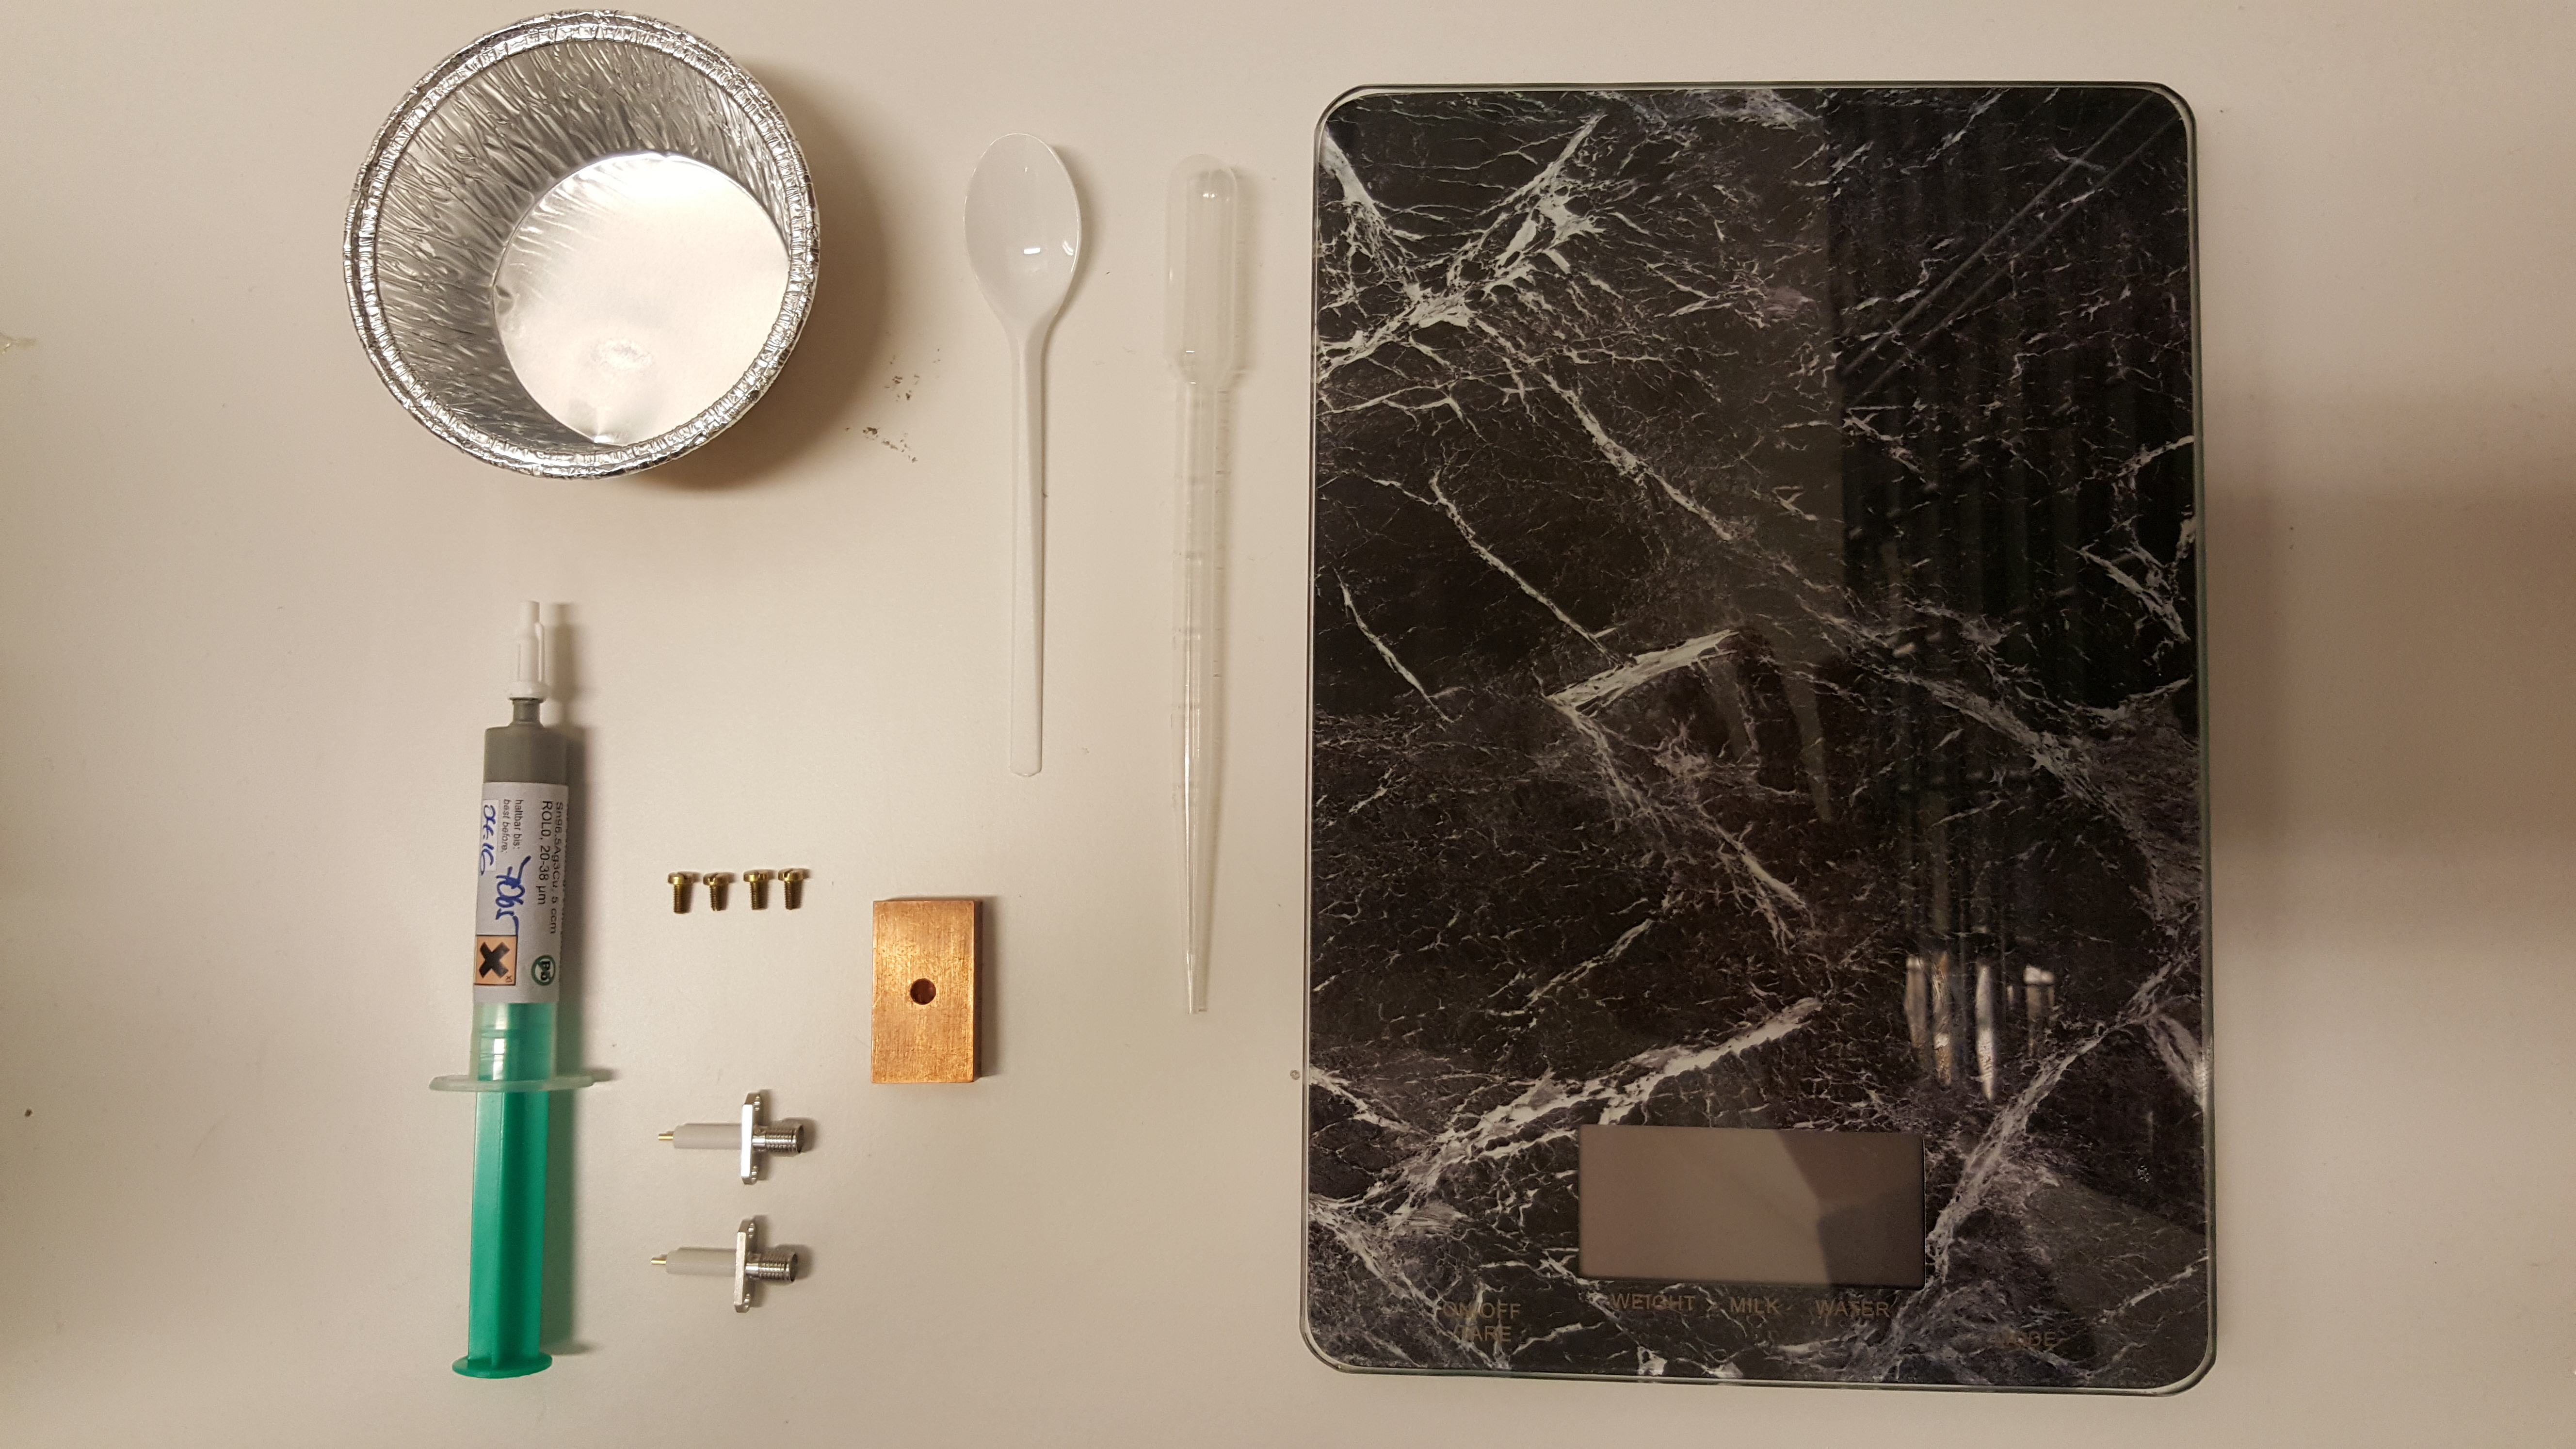
\includegraphics[width=0.65\textwidth]{figure/Filterbilder/filter_material.jpg}};
        \begin{scope}[x={(image.south east)},y={(image.north west)}]
            \node [anchor=west] (form) at (0.1,0.95) {\Large\textbf A};
            \node [anchor=west] (sked) at (0.35,0.935) {\Large\textbf B};
            \node [anchor=west] (pipett) at (0.425,0.925) {\Large\textbf C};
            \node [anchor=west] (paste) at (0.125,0.525) {\Large\textbf D};
            \node [anchor=west] (screws) at (0.255,0.46) {\Large\textbf E};
            \node [anchor=west] (SMA) at (0.315,0.18) {\Large\textbf F};
            \node [anchor=west] (filterbox) at (0.3777,0.32) {\Large\textbf G};
            \node [anchor=west] (scl) at (0.88,0.085) {\Large\textbf H};
        \end{scope}
    \end{tikzpicture}
    \caption{Material som behövs för att göra ett distribuerat lågpassfilter visas i figurer: blandningsform(A), sked(B), pipett(C), lödpasta(D), skruvar(E) för att fästa Radiall R124.464.000W SMA-kontakter(F) i filterlåda av koppar(G) och en våg(H).}
    \label{fig:filter_material}
\end{figure}

%Montering av filter kan delas upp i tre olika steg:


% översikt över det olika stegen borde finnas här ev mer utförligt
%\begin{enumerate}
%    \item Skala SMA kontakter
%    \item Montera och löda SMA kontakter
%    \item Förbereda Stycast och fylla filtret
%\end{enumerate}


Första steget i att göra ett filter är att förbereda SMA kontakterna. Detta innefattar att eventuellt skala av en del av teflonet från kontakten för att få den önskade längden på den frilagda ledaren som sedan ska inkapslas i Stycast. För att få den önskade längden på den frilagda ledaren skars först en bit eltejp till så att bredden på denna motsvarade längden på teflonet som skulle behållas. Eltejpen virades sedan runt SMA kontakten som i \figref{fig:f_SMA_skalning} och det frilagda teflonet skars bort med en hobbykniv. 

%%%%%%%%%%%%%%%%%%%%%%%%%%%%%%%%%%%%%%%%%%%%%%%%%%%%%%%%%
% Bild på SMA kontakt innan, under och efter den skalats
%%%%%%%%%%%%%%%%%%%%%%%%%%%%%%%%%%%%%%%%%%%%%%%%%%%%%%%%%
%0.329
\begin{figure}[h]
    \centering
    \begin{subfigure}{0.25\textwidth}
        \centering
        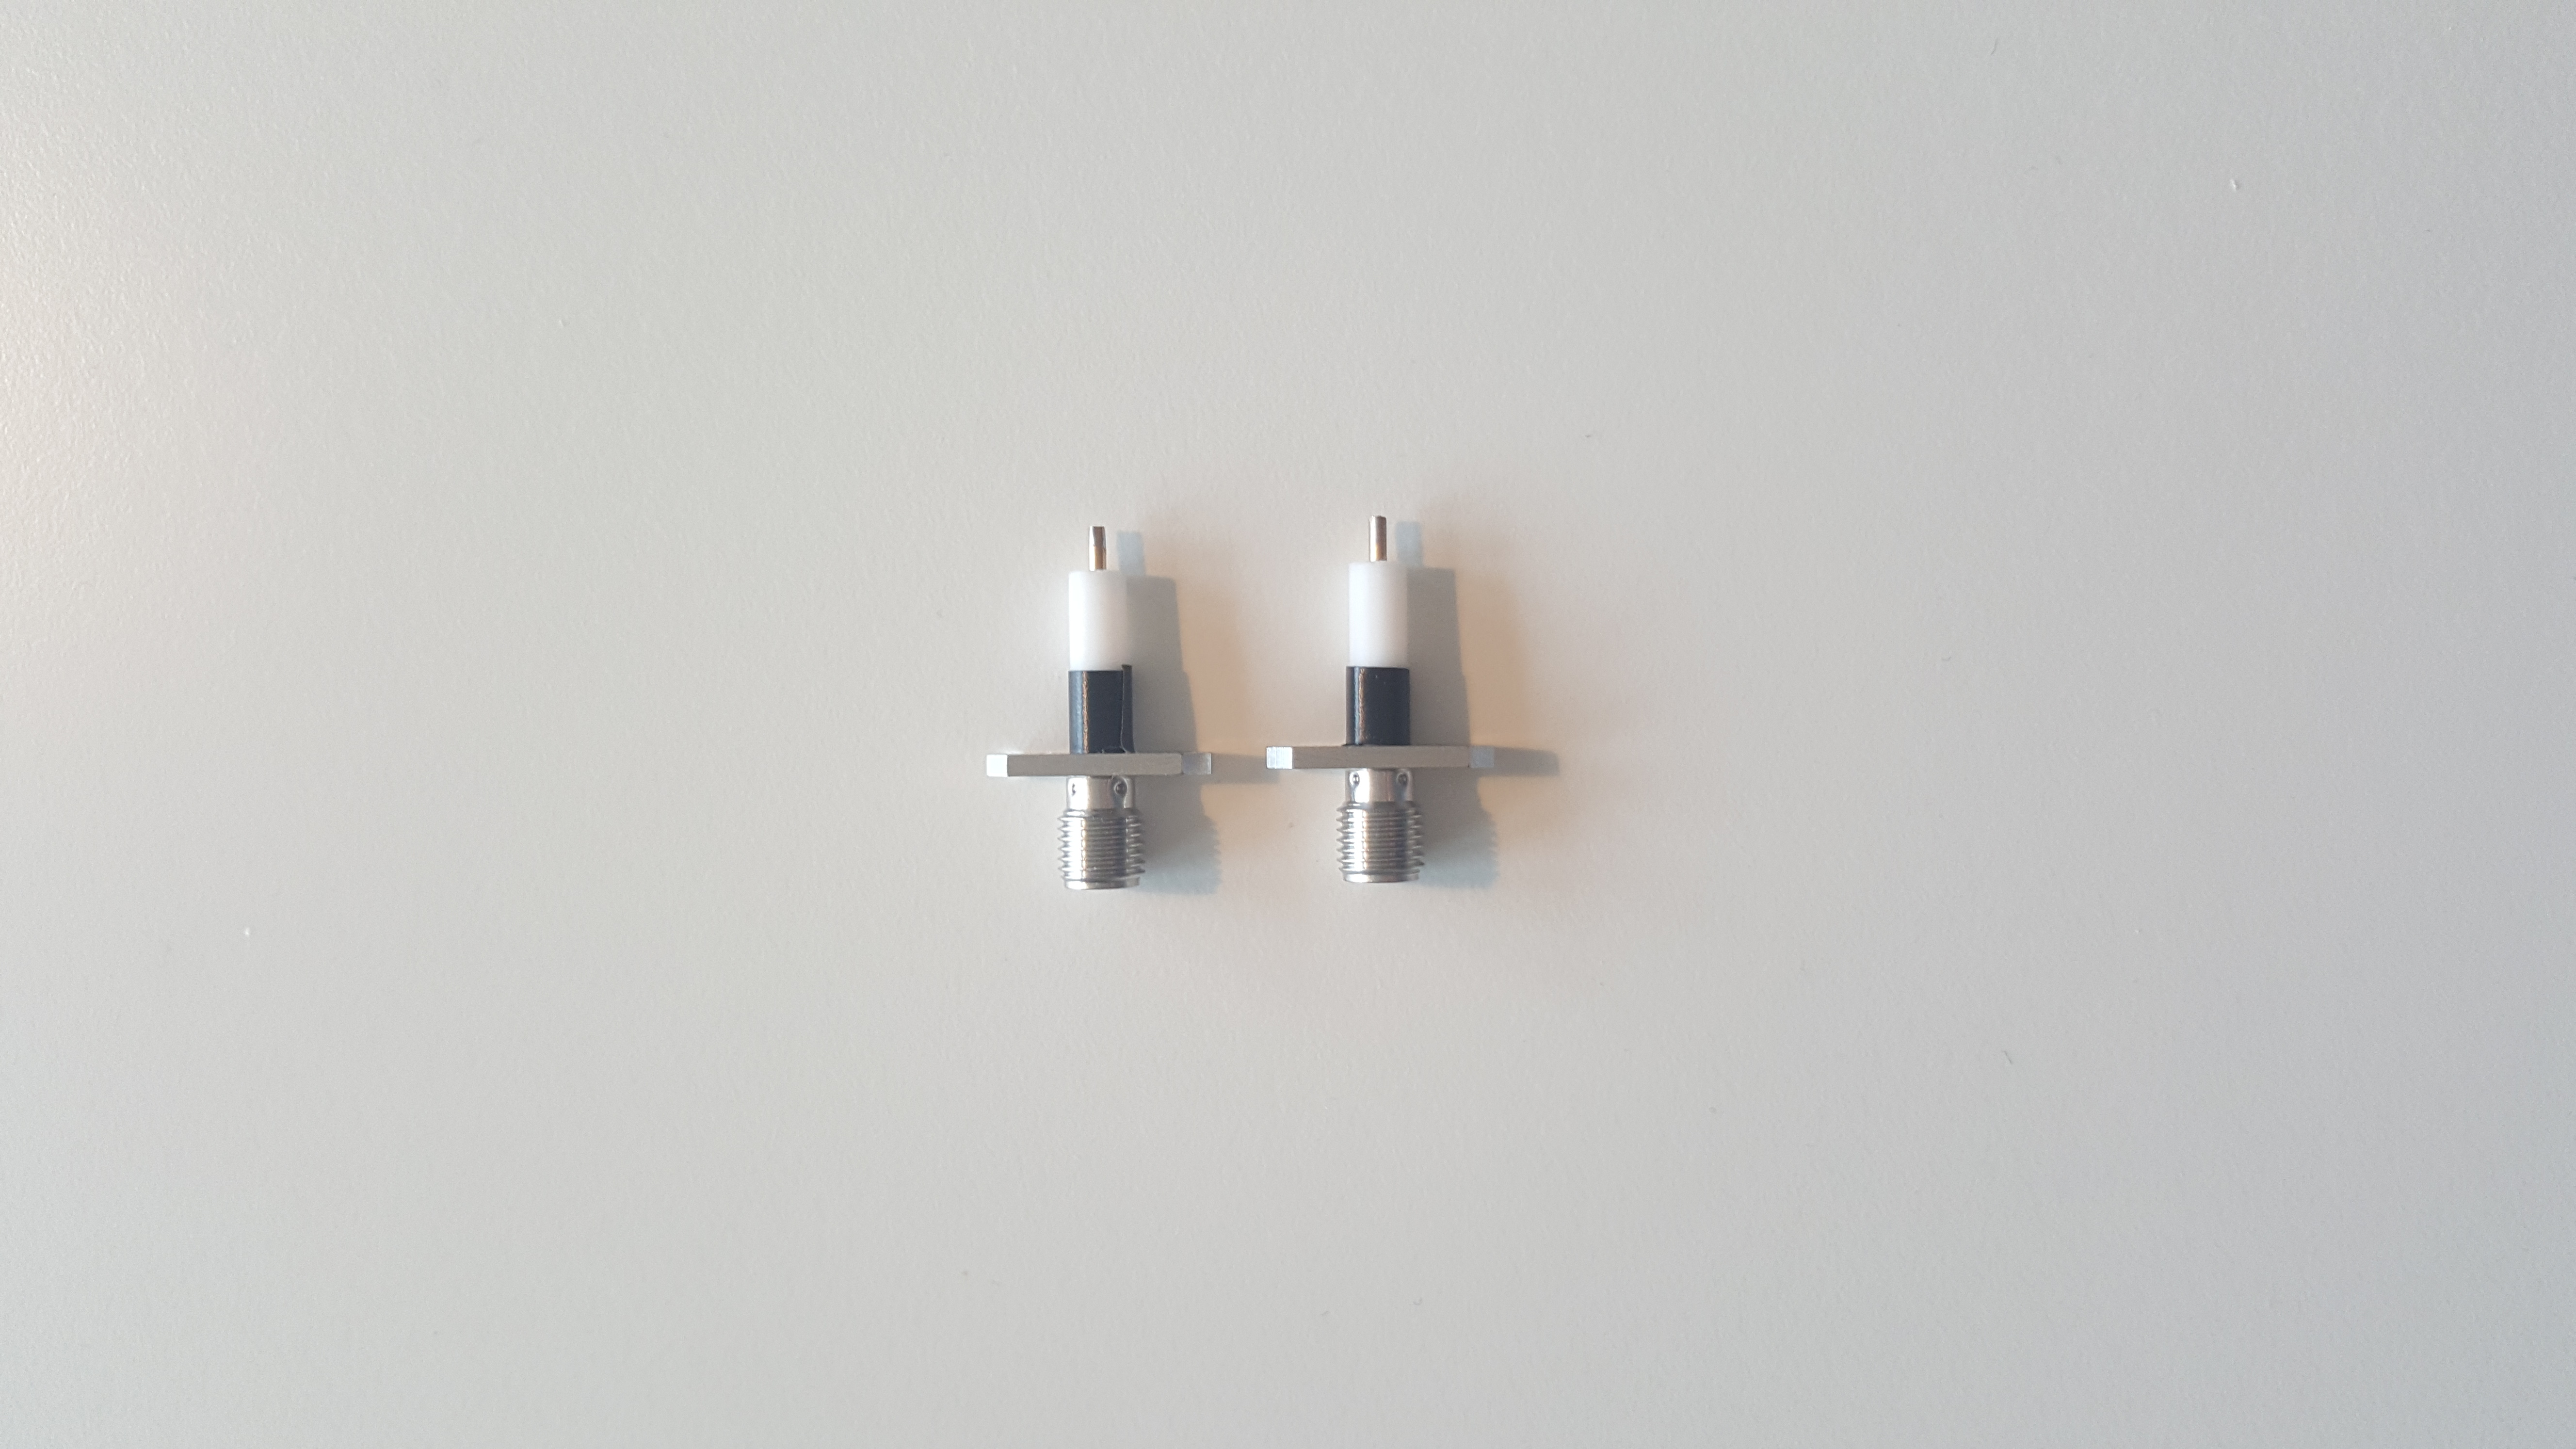
\includegraphics[angle=-90,trim=1450 100 1550 100,clip,width=0.97\linewidth]{figure/Filterbilder/f_sma_skalning.jpg} 
        \caption{}
        \label{fig:f_SMA_skalning}
    \end{subfigure}
        \begin{subfigure}{0.25\textwidth}
        \centering
        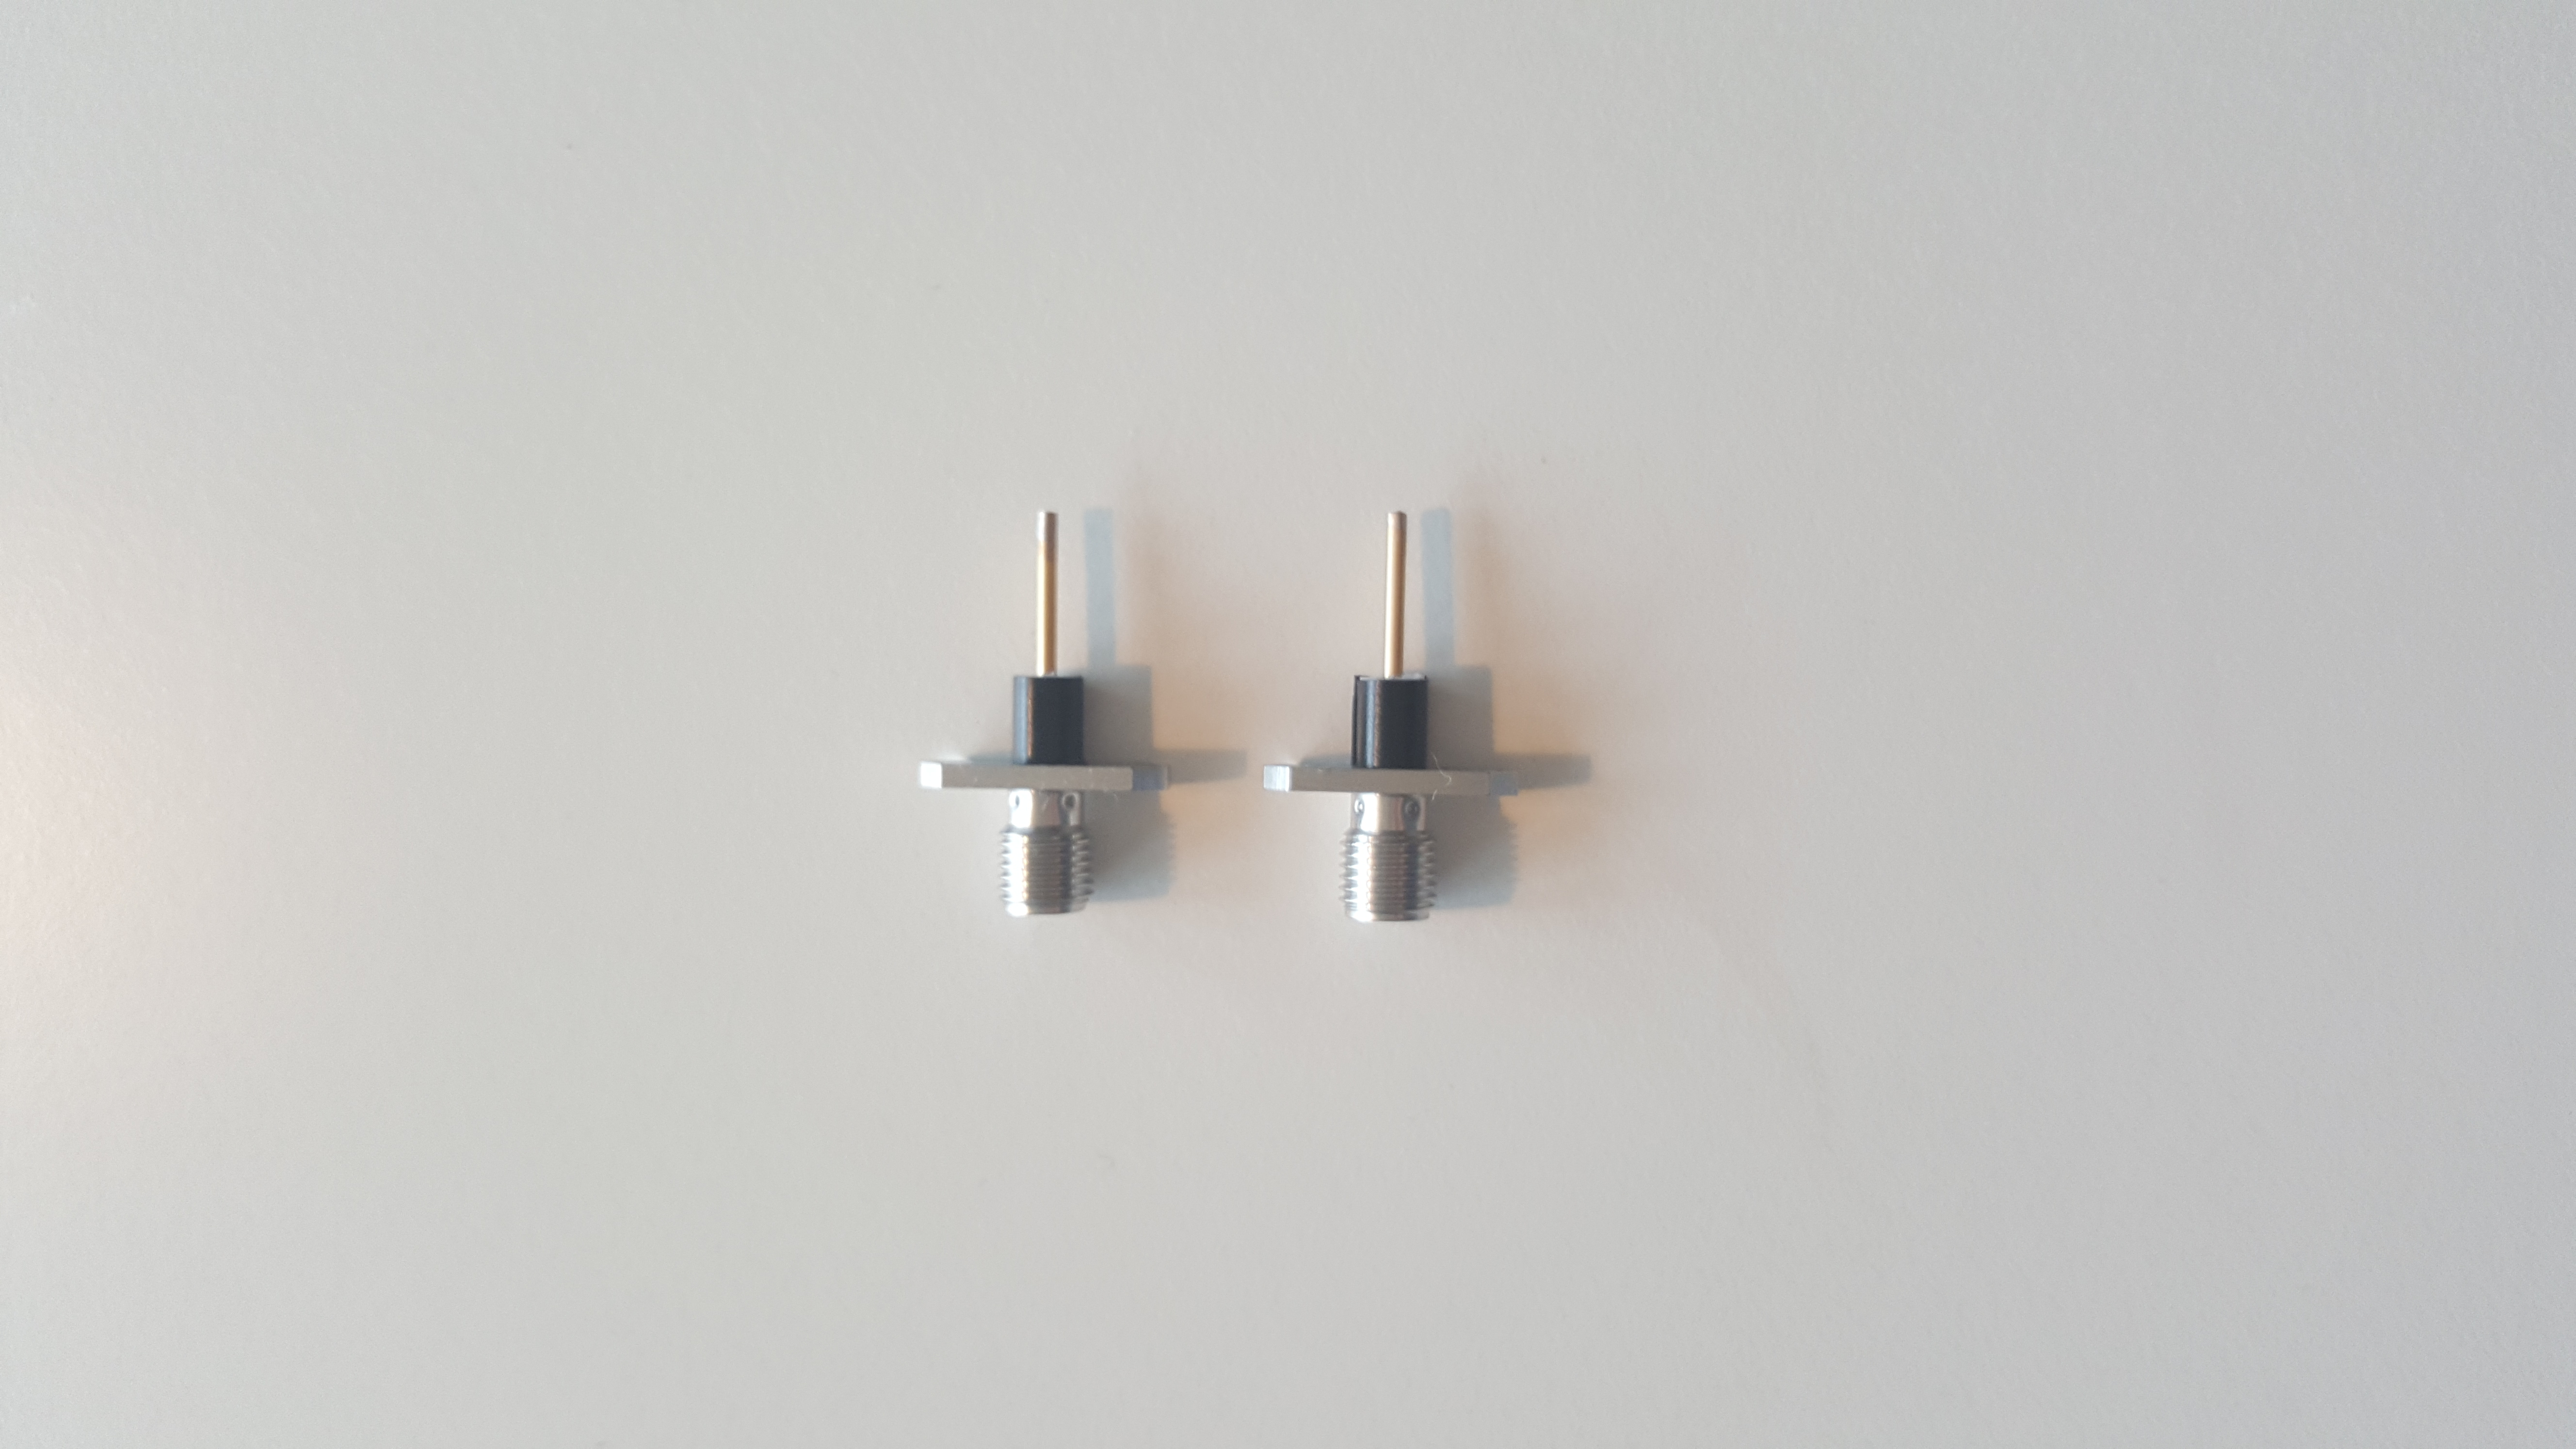
\includegraphics[angle=-90,trim=1450 100 1550 100,clip,width=0.97\linewidth]{figure/Filterbilder/u_sma_skalning.jpg} 
        \caption{}
        \label{fig:u_SMA_skalning}
    \end{subfigure}
        \begin{subfigure}{0.25\textwidth}
        \centering
        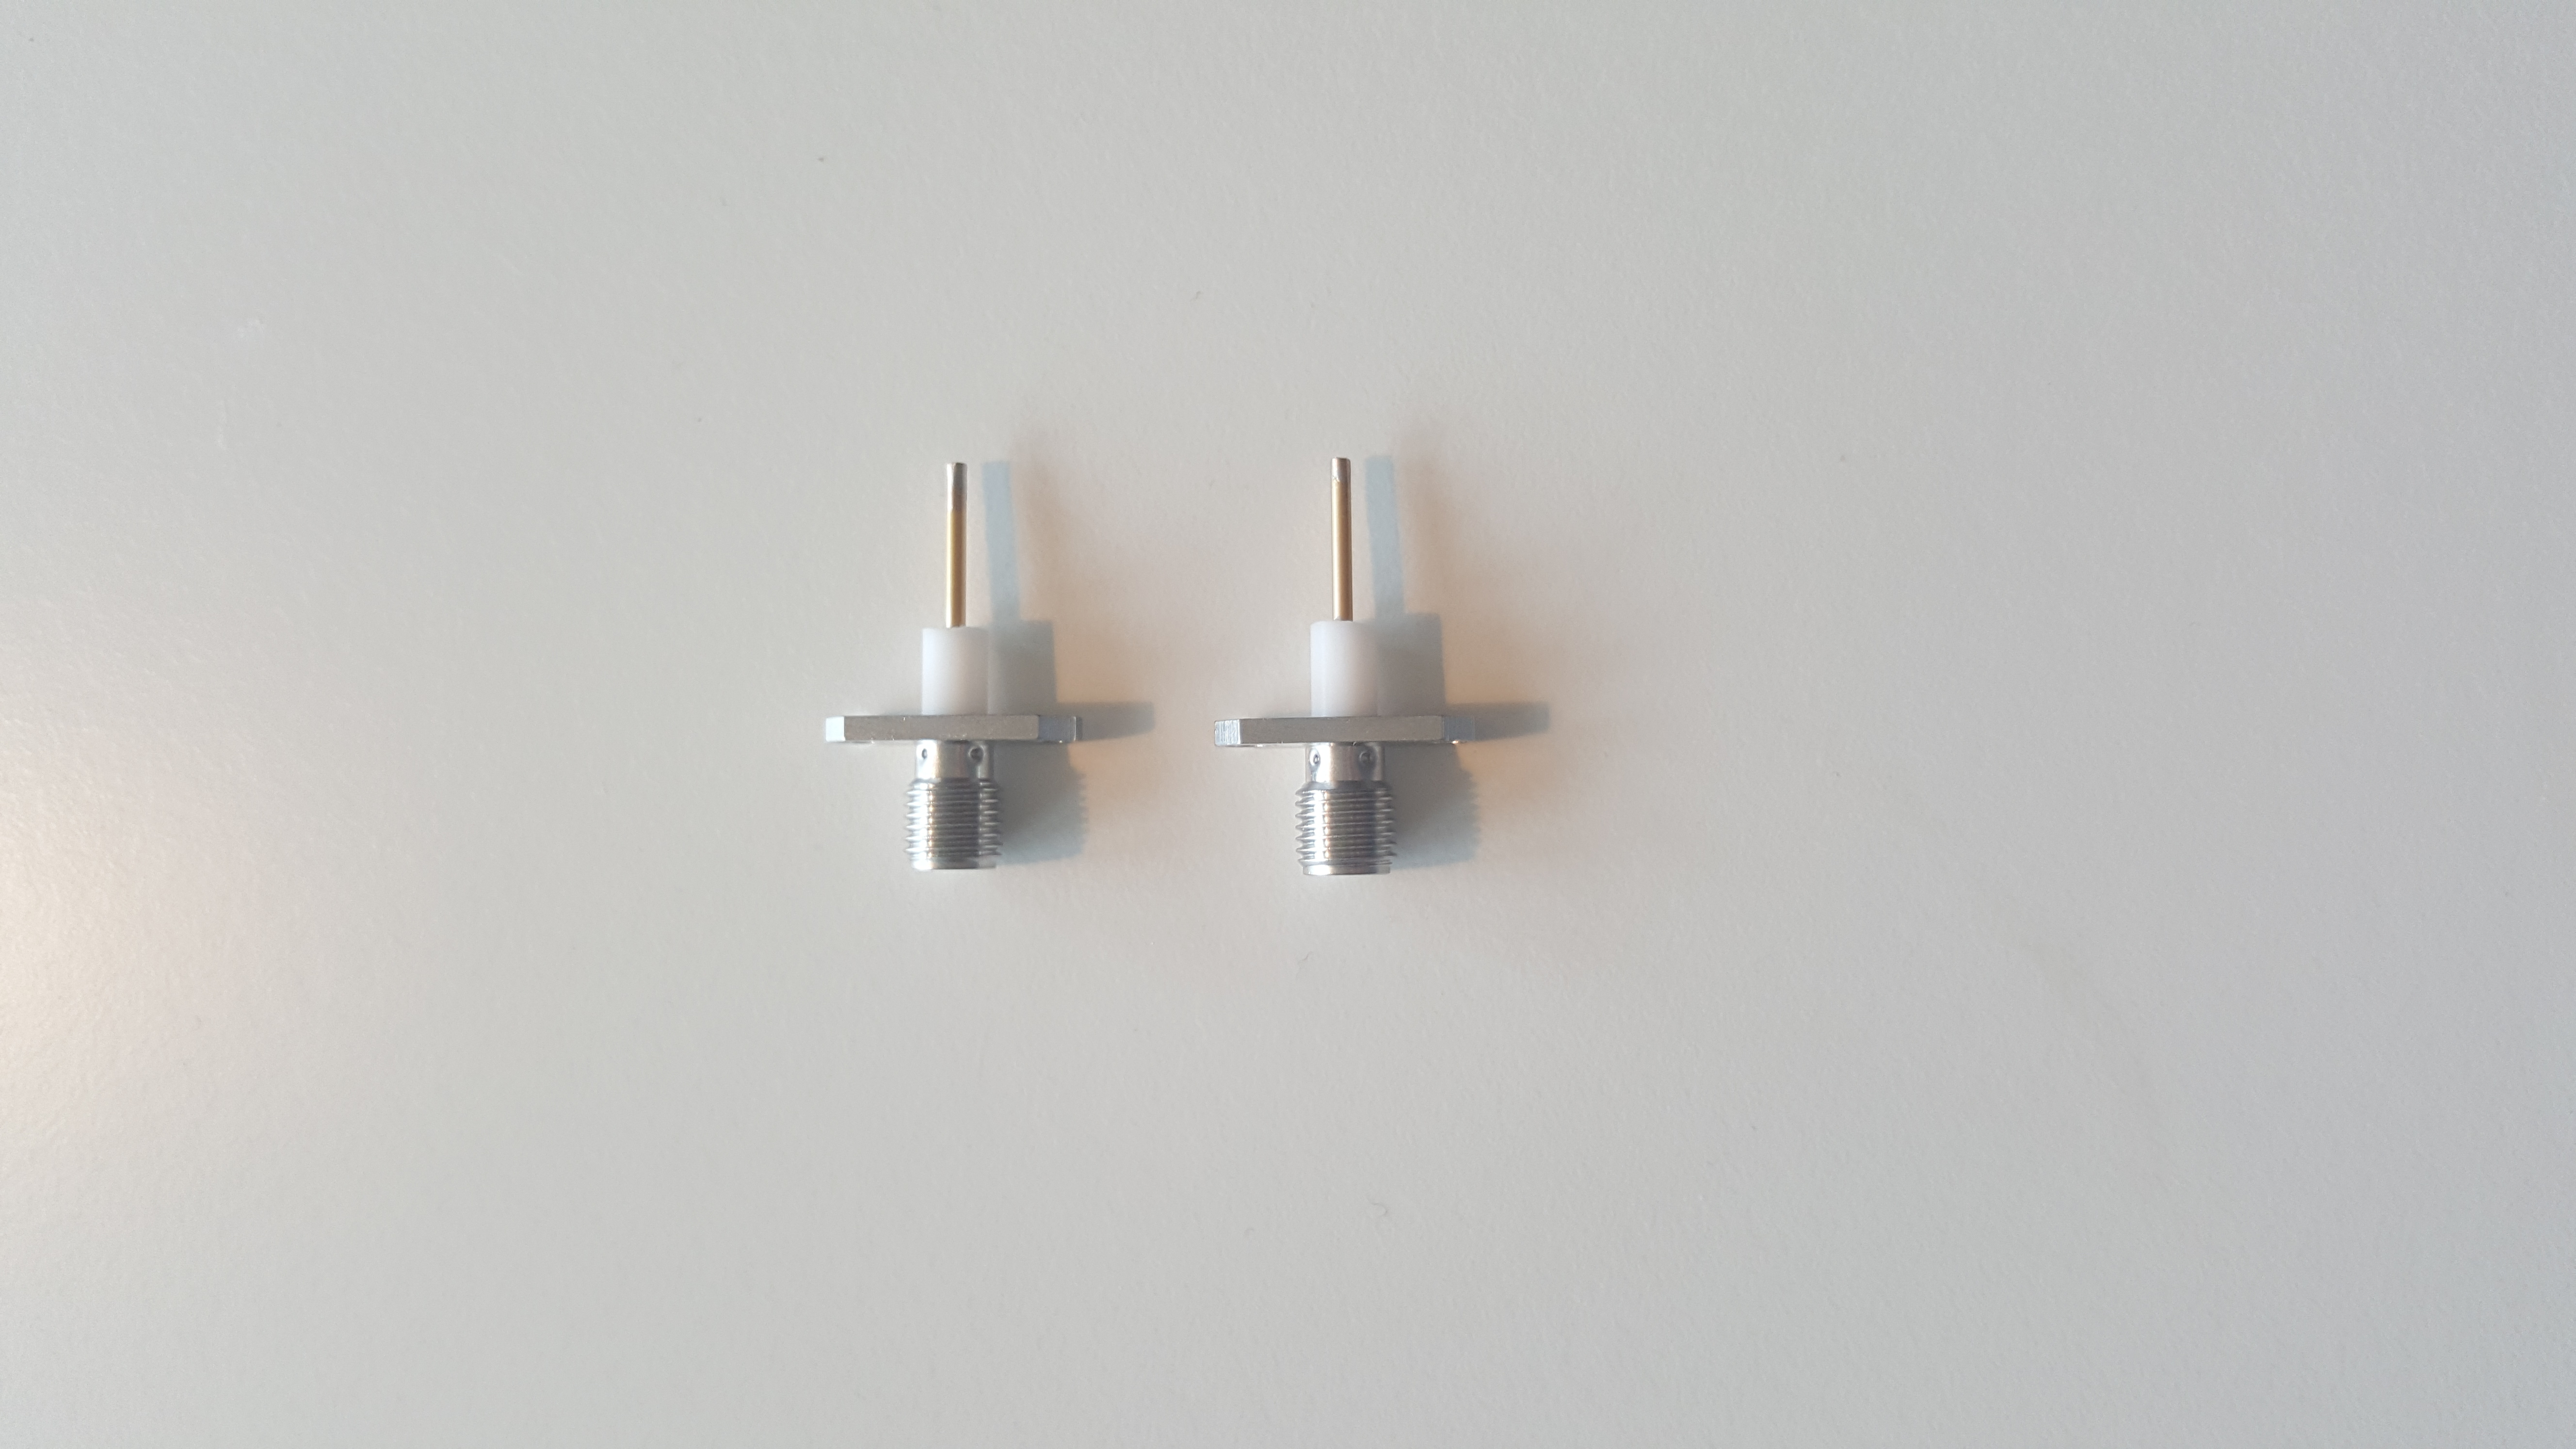
\includegraphics[angle=-90,trim=1300 100 1700 100,clip,width=0.97\linewidth]{figure/Filterbilder/e_sma_skalning.jpg} 
        \caption{}
        \label{fig:e_SMA_skalning}
    \end{subfigure}
    
    
    \caption{Bilden visar de olika stegen i att förbereda SMA-kontakter för att få den önskade längden på den frilagda ledaren. Först virades eltejp runt teflonet som skulle behållas som i \subref{fig:f_SMA_skalning} och därefter skars de frilagda teflonet bort \subref{fig:u_SMA_skalning}. De färdiga SMA-kontakterna visas i \subref{fig:e_SMA_skalning}.}
    \label{fig:SMA_skalning}
\end{figure}

Efter att SMA kontakterna har skalats av till önskad längd så kan dessa monteras i det maskinarbetatade kopparblocket. Först applicerades en liten mängd lödpasta på den ena SMA kontakten som i \figref{fig:prep_SMA} och därefter fördes båda SMA kontakterna in i kopparlådan och skruvades fast. Lödpastan ska omsluta båda ledarna som i \figref{fig:filter_soldering} och de båda ledarna bör vara koaxiala för att minska reflektioner. 

För att löda ihop SMA kontakterna användes en lödkolv med en mejsel-spets för att kunna få bra termisk kontakt mellan de två ledarna och lödpastan. Lödkolven fördes in genom titthålet på kopparlådans översida och placerades mot de två ledarna tills dess att lödpastan smält och flutit ut så att lödningen ser ut som i \figref{fig:post_solder}.

%Därefter kontrollerades lödningens kvalité genom att mäta $S_{21}$-parametern för filtret med VNA i frekvensintervallet \unit[1-50]{GHz}. Magnituden hos $S_{21}$ undersöktes sedan för kraftiga spikar som ett resultat av dåligt matchad impedans, vilket skulle indikera på en dålig lödning. Resultat från dessa mätningar presenteras i \ref{sec:filter_kar}. 

%%%%%%%%%%%%%%%%%%%%%%%%%%%%%%%%%%%%%%%%%%%%%%%%%%%%%%%%%
% Bild på SMA kontakter innan och efter lödning
%%%%%%%%%%%%%%%%%%%%%%%%%%%%%%%%%%%%%%%%%%%%%%%%%%%%%%%%%

\begin{figure}[h]
    \centering
    \begin{subfigure}{0.25\textwidth}
        \centering
        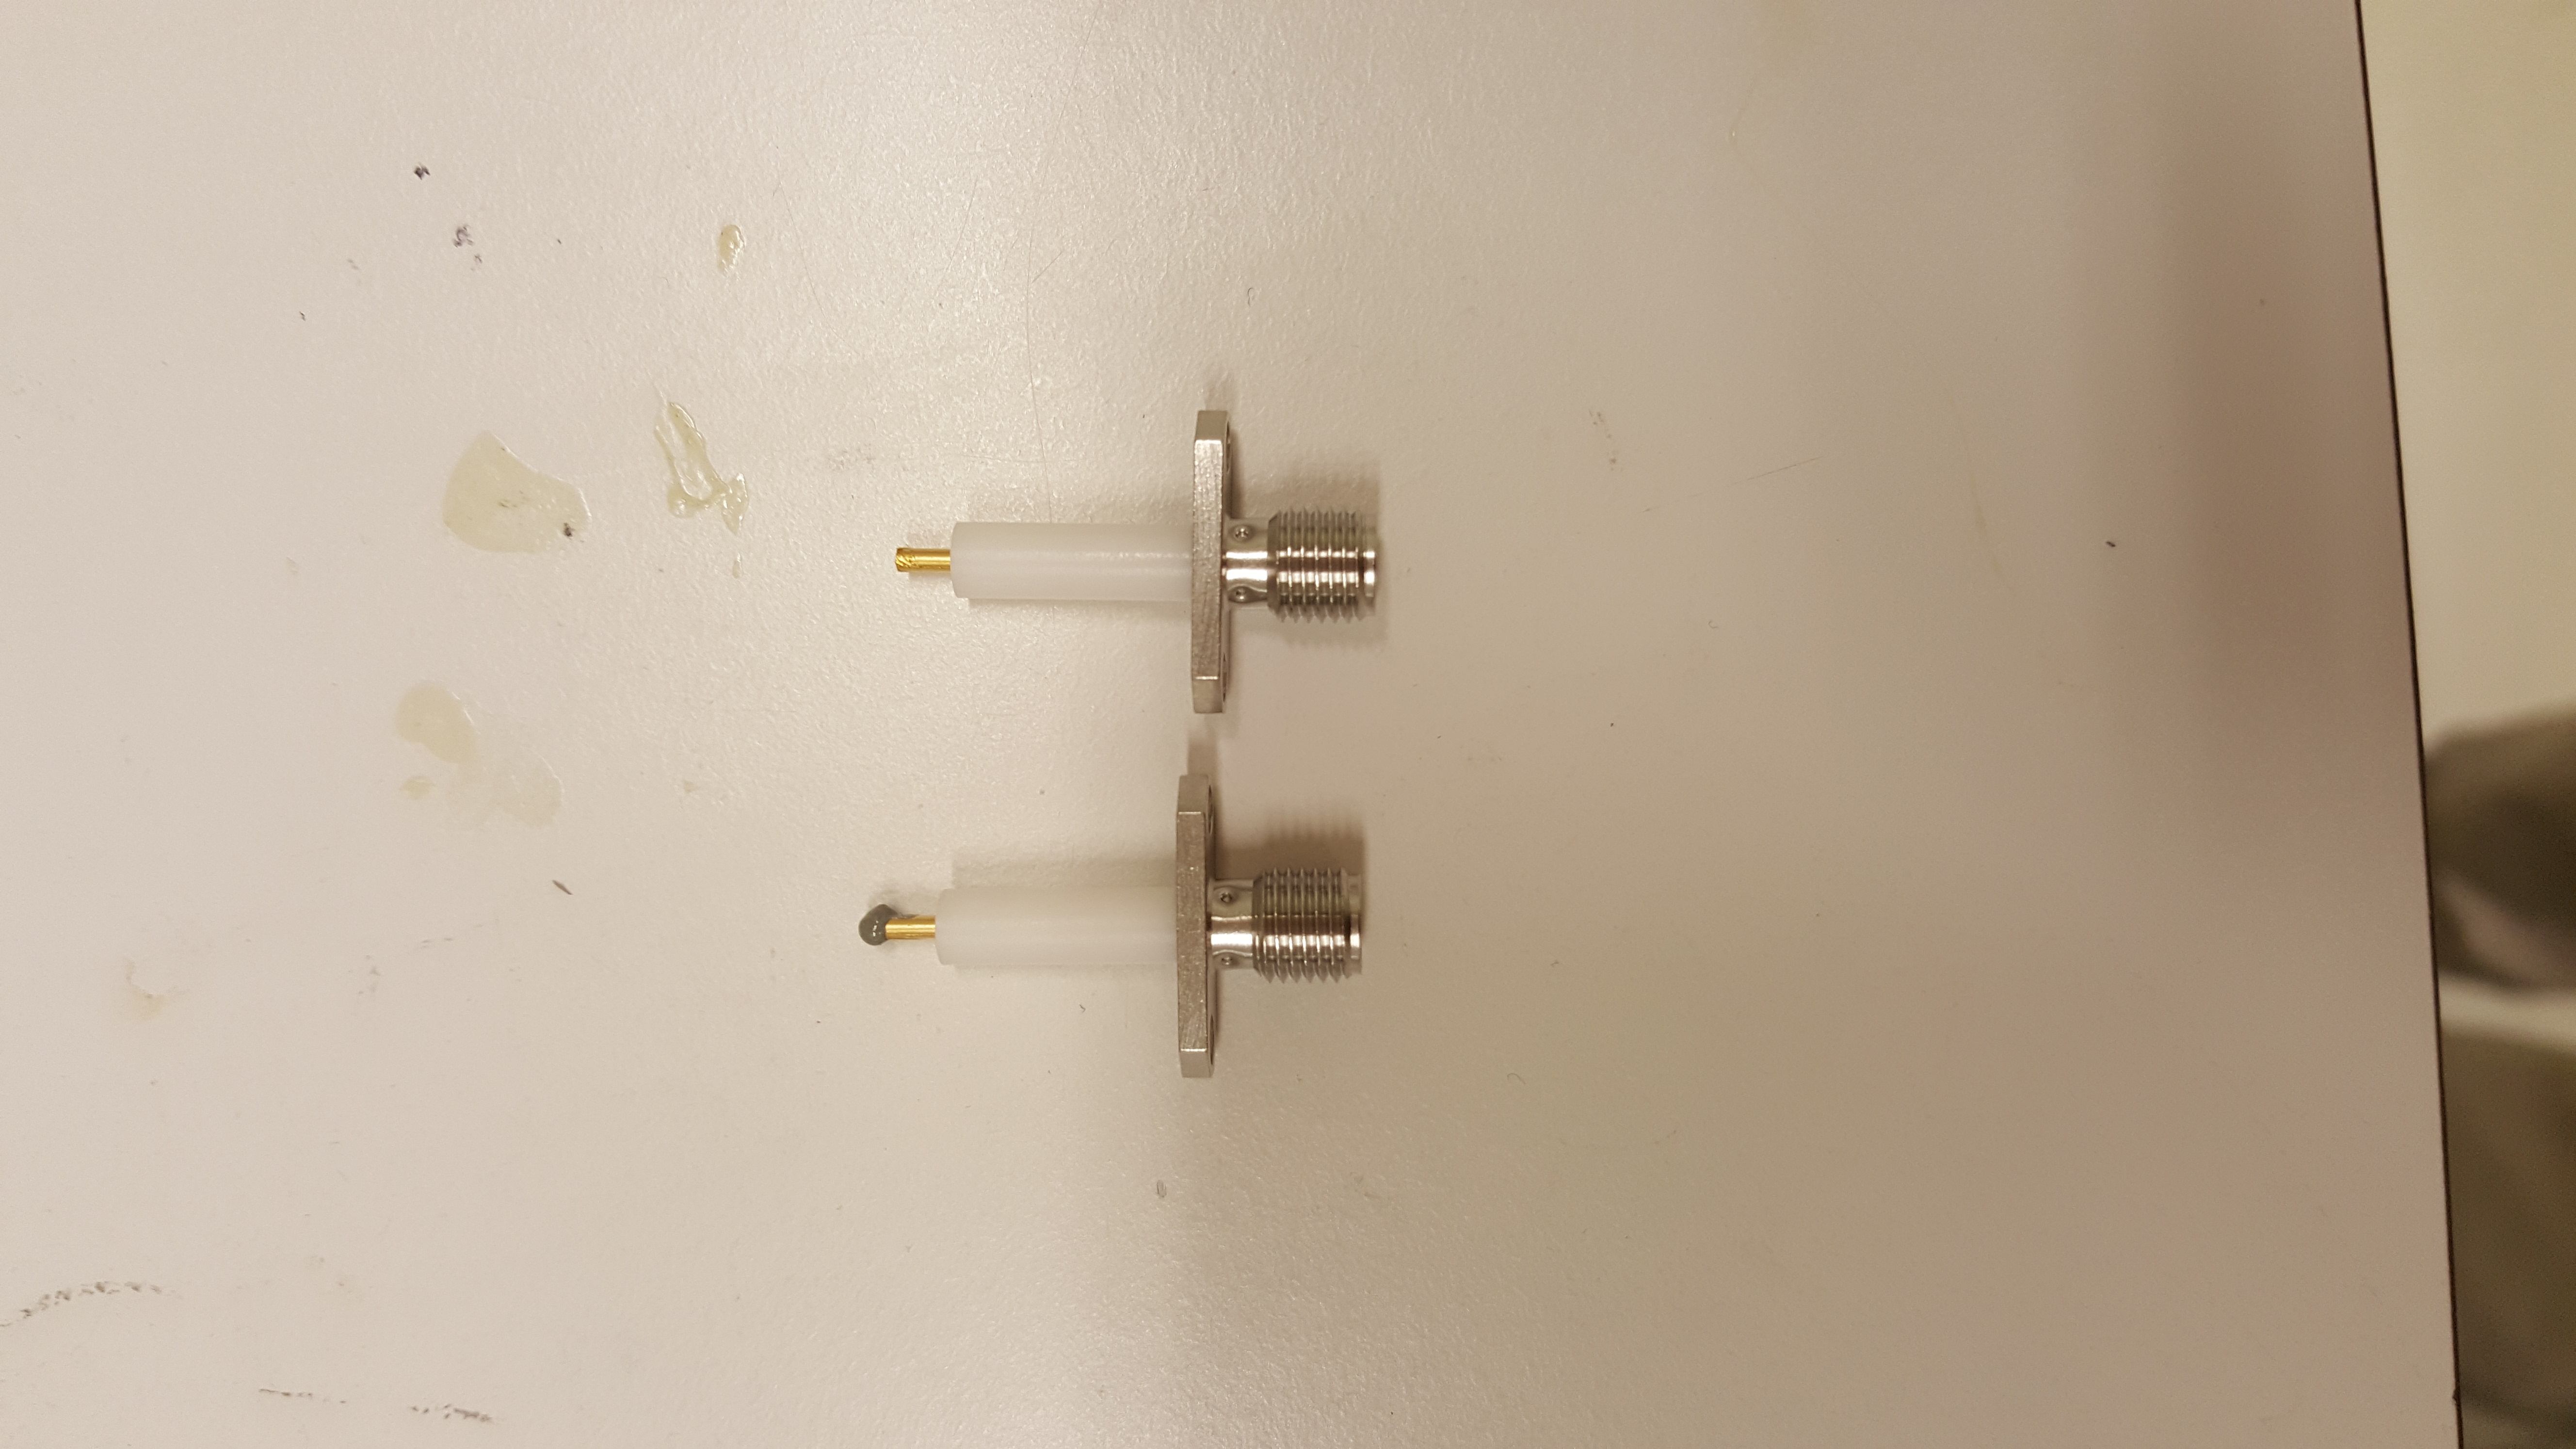
\includegraphics[angle=-90,trim=1200 100 1800 100,clip,width=0.97\linewidth]{figure/Filterbilder/prep_SMA.jpg} 
        \caption{}
        \label{fig:prep_SMA}
    \end{subfigure}
    \begin{subfigure}{0.25\textwidth}
        \centering
        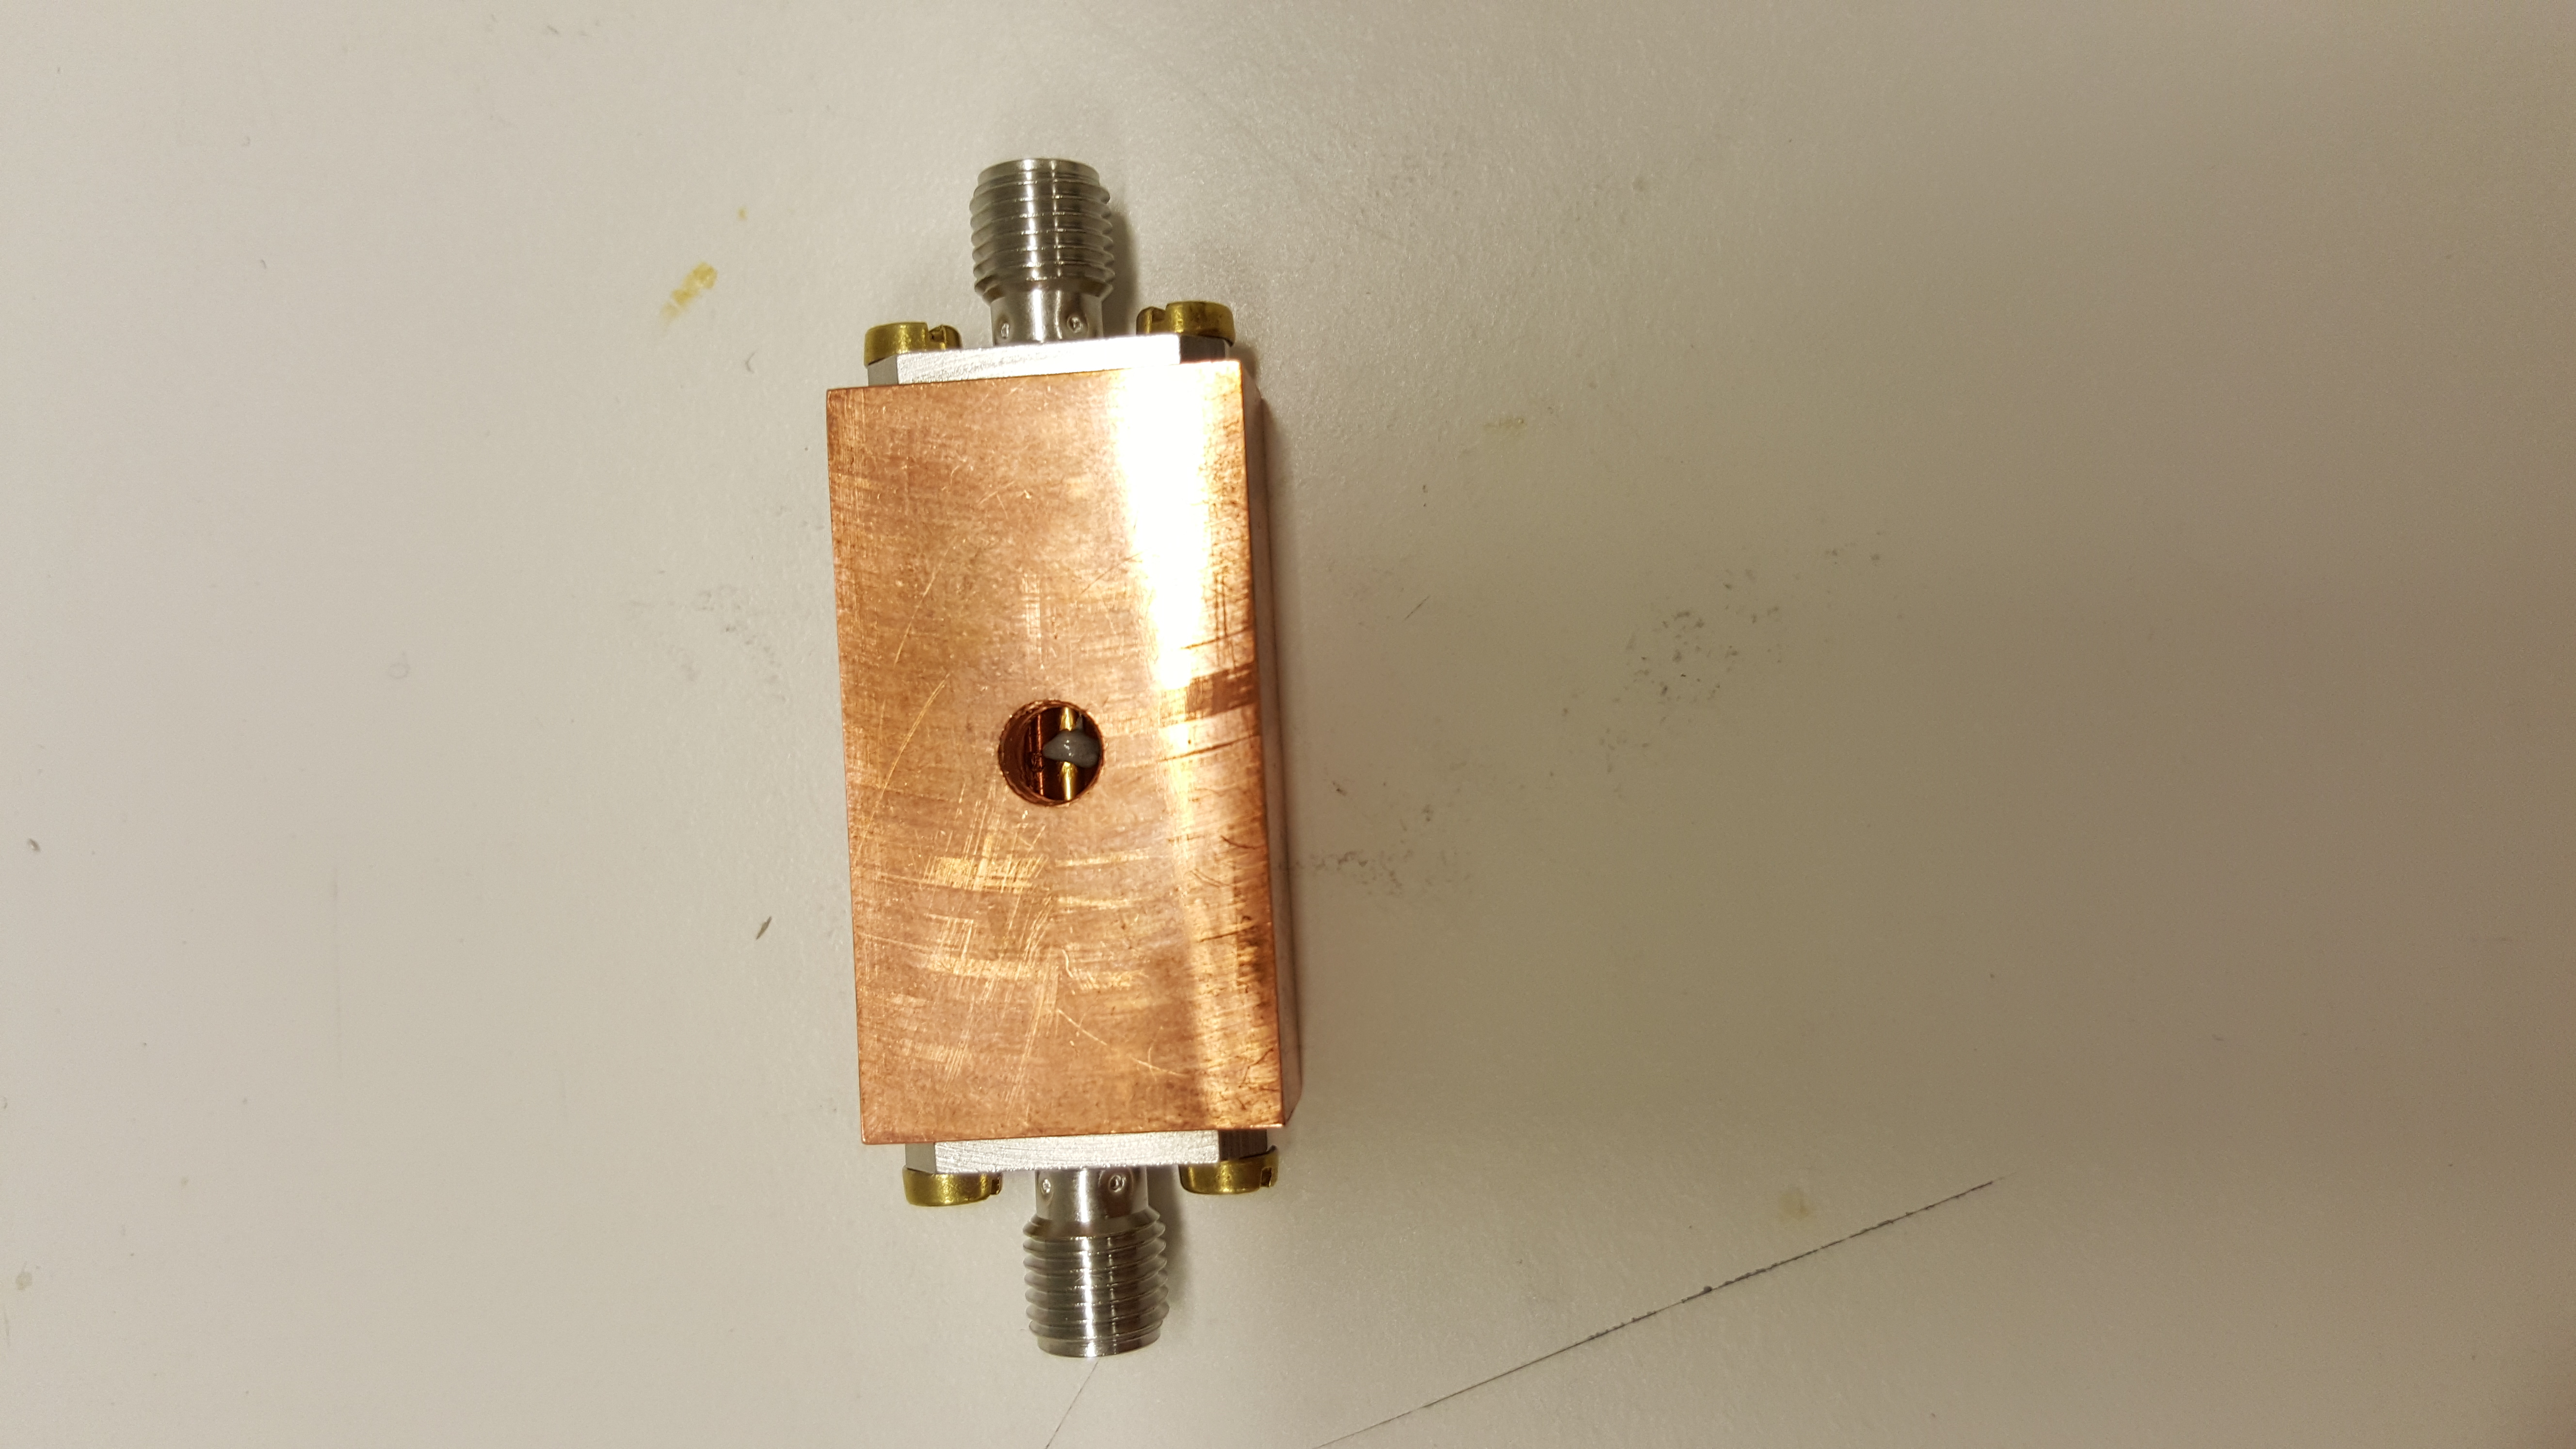
\includegraphics[angle=-90,trim=1000 100 2000 100,clip,width=0.97\linewidth]{figure/Filterbilder/filter_before_solder.jpg} 
        \caption{}
        \label{fig:before_solder}
    \end{subfigure}
    \begin{subfigure}{0.25\textwidth}
        \centering
        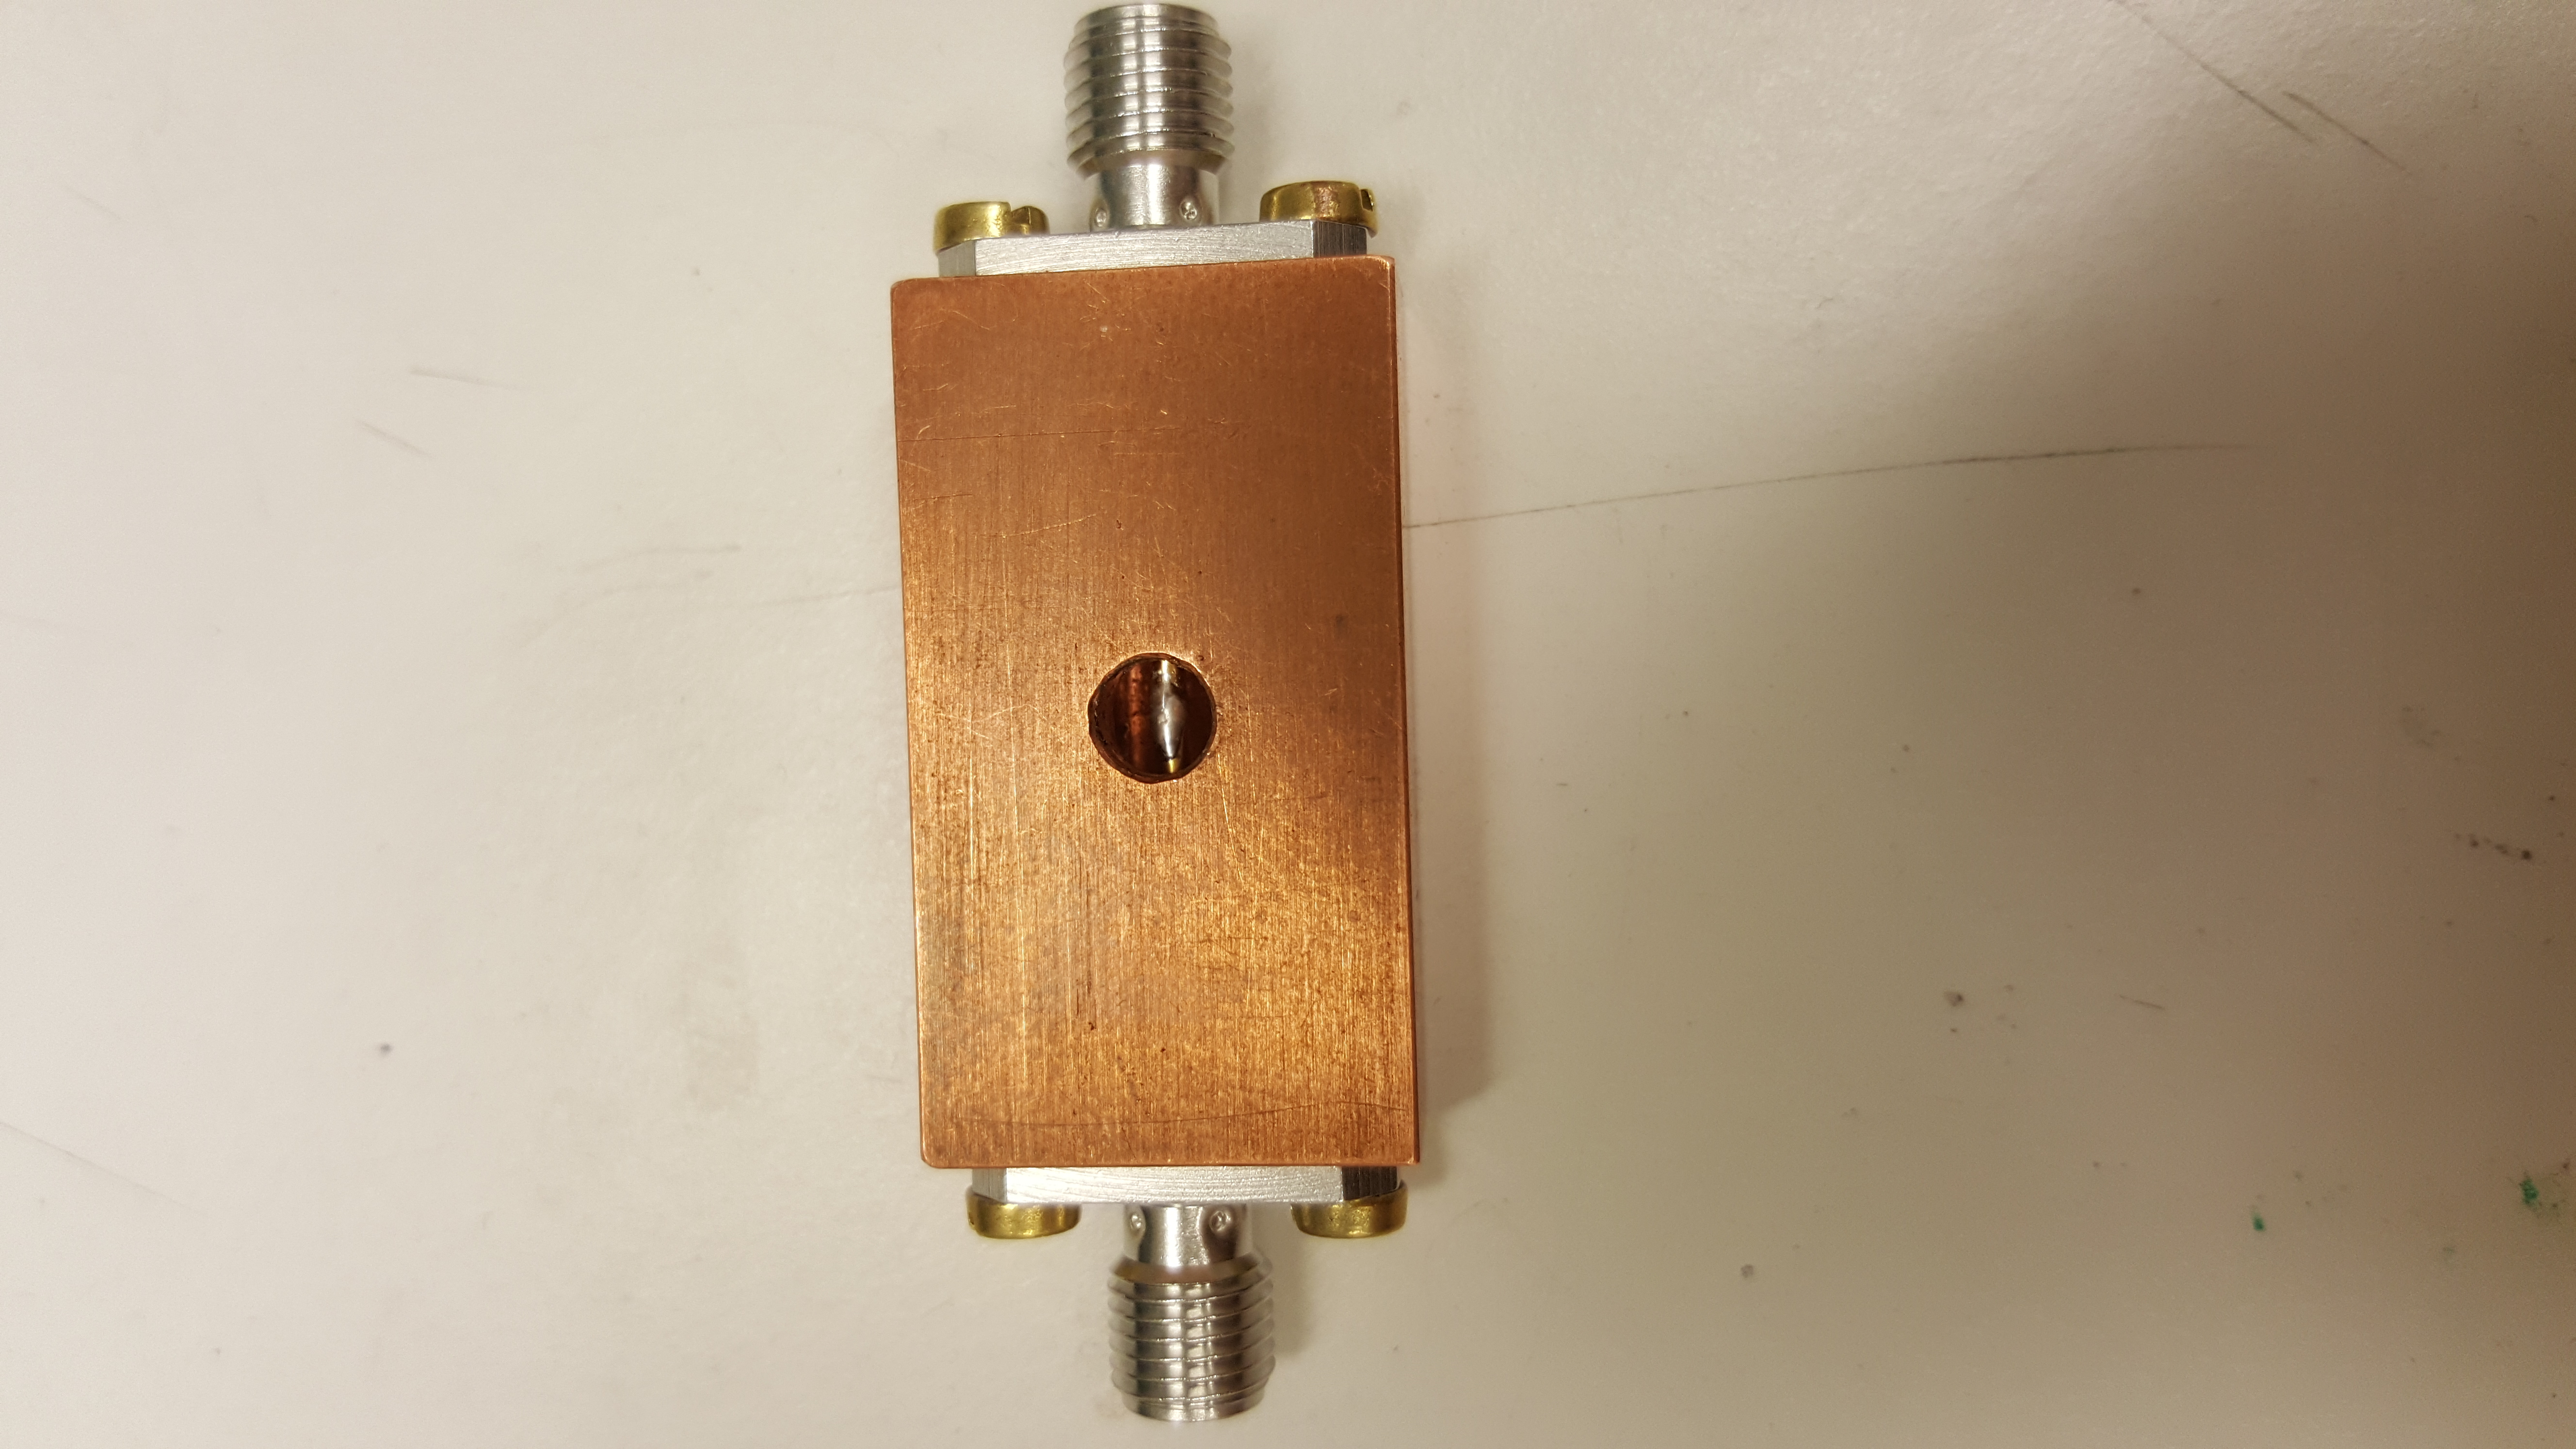
\includegraphics[angle=-90,trim=1200 100 1800 100,clip,width=0.97\linewidth]{figure/Filterbilder/filter_post_solder.jpg} 
        \caption{}
        \label{fig:post_solder}
    \end{subfigure}
    
 \caption{I bilden visas de olika stadierna för att löda ihop ett distribuerat lågpassfilter. I \protect\subref{fig:prep_SMA} har en liten mängd lödpasta applicerats på den vänstra SMA-kontakten. Efter att SMA-kontakterna förts in i koppparlådan så bör lödpastan omsluta båda ledaran som i \subref{fig:before_solder}. I \subref{fig:post_solder} visas den färdiga lödningen.}
 \label{fig:filter_soldering}
\end{figure}


% Måste få in i texten någonstans att förhållandet mellan de olika delarna ska vara A 100:28 B
Efter att lött ihop SMA-kontakterna placerades filtret på en värmeplatta vid \unit[40]{$^\circ$C} för att underlätta när filtret senare ska fyllas med Stycast genom att sänka dess viskositet. Därefter blandades \unit[12,8]{g} Stycast genom att först väga upp \unit[10]{g} Stycast del A och \unit[2,8]{g} Stycast del B och sedan blanda ihop dessa till en homogen vätska i en metallform med hjälp av en plastsked. 

\begin{wrapfigure}{r}{0.25\textwidth}
    \centering
    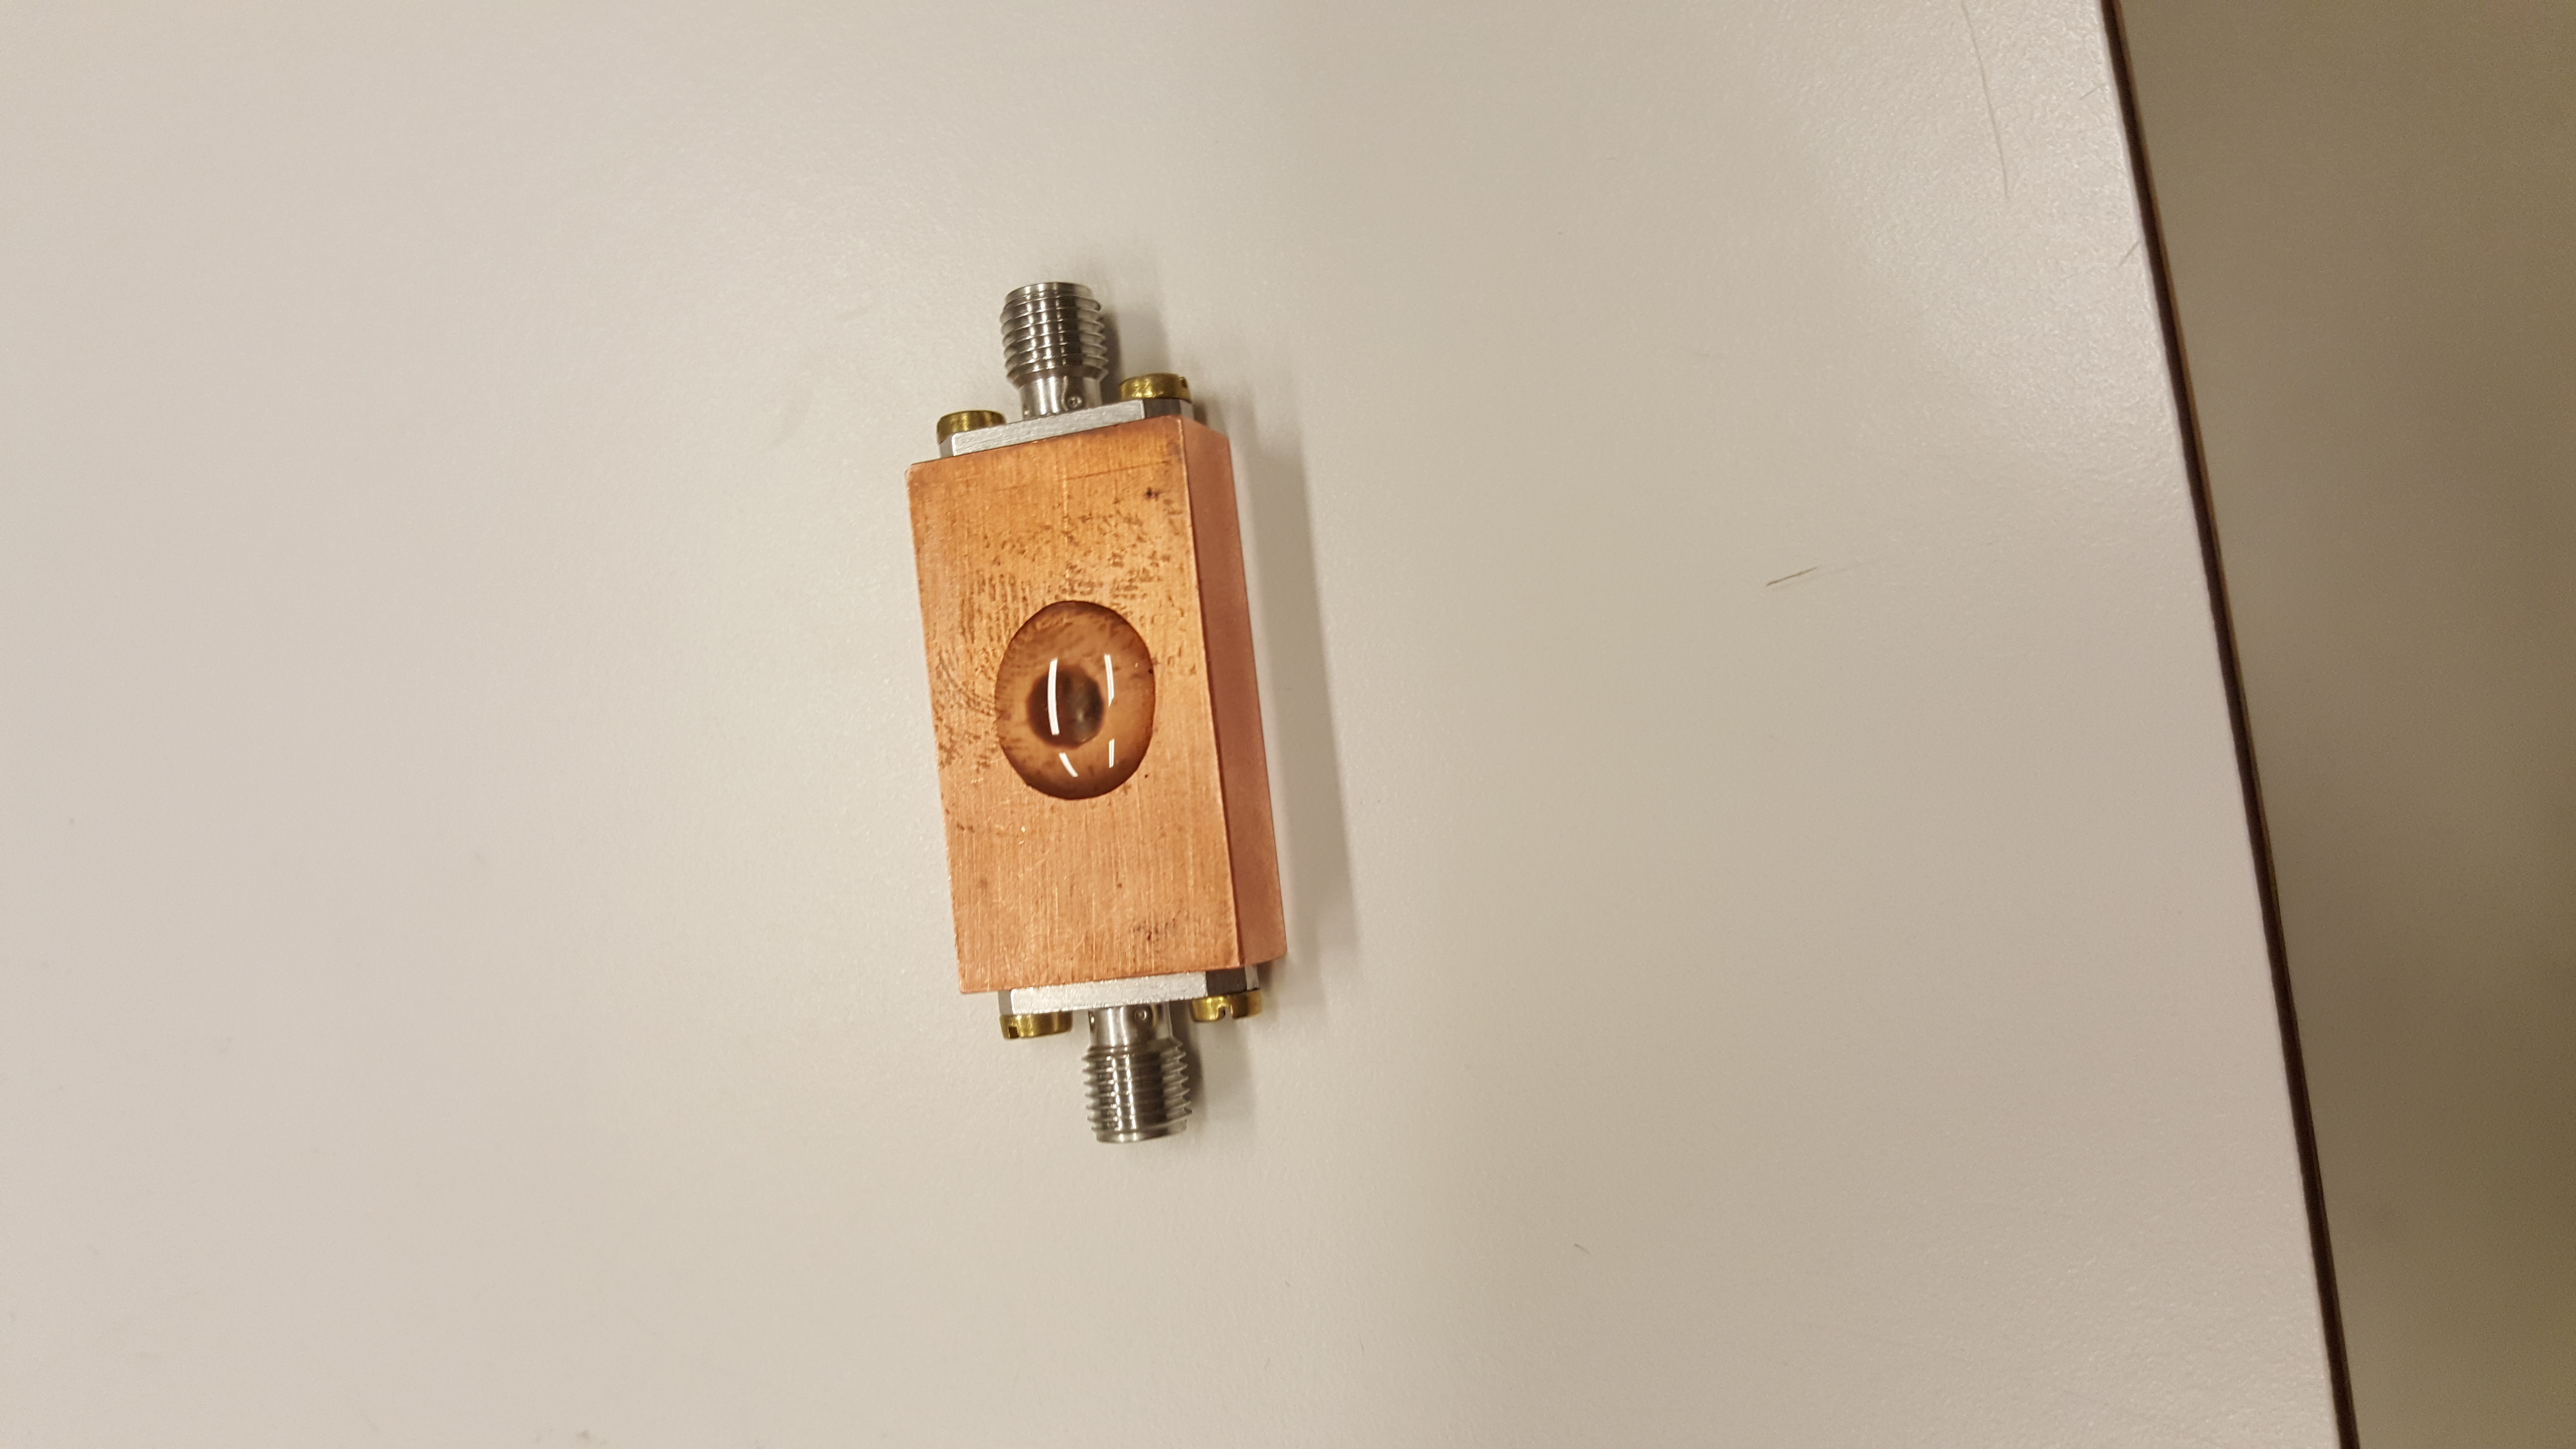
\includegraphics[angle=-90,trim=1250 200 1950 200,clip,width=0.975\linewidth]{figure/Filterbilder/stycast_fill.jpg}
    \caption{Filter som fyllts med Stycast med en stor droppe stycast över titthålet.}
    \label{fig:stycast_filled}
\end{wrapfigure}

Till ett filter går det åt ungefär \unit[$\approx 2$]{g} Stycast beroende på hur lång ledaren som ska kapslas in är. Det är dock nödvändigt att blanda åtminstone \unit[10]{g} för att försäkra sig om att att blandningen är homogen och att förhållandet mellan del A och del B är korrekt. 

Filtret fylldes sedan försiktigt med Stycast med hjälp av en pipett. Pipetten placerades mot kanten av titthålet och Stycast pressades ut långsamt för att förhindra att en bubbla över titthålet bildades, vilket skulle hindra luften i filtret från att kunna komma ut. 

Efter att filtret var fullt placerades en stor droppe Stycast över titthålet som i \figref{fig:stycast_filled} så att ifall det fortfarande fanns lite luft kvar i filtret så skulle detta kunna komma ut och den extra Stycasten som placerades över titthålet skulle kunna fylla igen hålrummet. Filtret härdades sedan vid rumstemperatur i minst 16 timmar. Efter att filtret härdats kan överflödigt Stycast på filtrets ovansida slipas bort. Detta är dock inte nödvändigt för filtrets funktion.


% Filterkarakteristik hade kunnat skippas om vi verkligen behöver sidor
\section{Filterkarakteristik}
\label{sec:filter_kar}
I detta projekt har vi konstruerat filter av tre olika längder i tre uppsättningar och vi kommer fortsättningsvis hänvisa till dessa enligt tabell \ref{tab:filter_list}.

\begin{table}[h]
    \centering
    \caption{Tabell över de individuella filterlängderna samlade i tre olika kategorier: kort, medel och lång.}
    \label{tab:filter_list}
    \begin{tabular}{llll}\toprule
        Namn & \multicolumn{3}{c}{Filterlängd (\unit{cm})} \\
        \midrule
        Kort & 1,895 & 1,88 & 1,825 \\
        Medel & 2,52 & 2,48 & 2,47 \\
        Lång & 3,145 & 3,155 & 3,15\\
        \bottomrule
    \end{tabular}
\end{table}

För att karakterisera samtliga filter användes en Agilent E8364B VNA. Filter anslöts direkt till VNA:n med två SMA M-M adapter och därefter mättes $S_{21}$ i frekvensintervallet \unit[1-50]{GHz}. Mätningen utfördes även innan filtrerna fylldes med Stycast. En mätning av $S_{21}$ utan filter togs också för att använda som referens. Denna referens motsvarar således kablarnas och adapternas påverkan på $S_{21}$, vilket gör det möjligt att särskilja filtrets dämpning från andra dämpande effekter i uppkopplingen.% som skinneffekt och reflektioner på grund av impedansmissmatcher. 

I \figref{fig:filter_kar} visas den uppmätta $|S_{21}|$ för ett filter, innan och efter det fylldes med Stycast, från varje kategori samt en referens. För resterande filter se appendix \ref{}.

\begin{figure}[H]
    \centerfloat
    \begin{subfigure}[t]{0.329\textwidth}
        \centerfloat
        \setlength\figurewidth{0.8\linewidth}
        \setlength\figureheight{11em}
        % This file was created by matlab2tikz.
%
\definecolor{mycolor1}{rgb}{0.1253 0.3242 0.8303}%
\definecolor{mycolor2}{rgb}{0.9990 0.7653 0.2164}%
\definecolor{mycolor3}{rgb}{0.1801 0.7177 0.6424}%
%
\begin{tikzpicture}[%
trim axis left, trim axis right
]

\begin{axis}[%
width=0.951\figurewidth,
height=\figureheight,
at={(0\figurewidth,0\figureheight)},
scale only axis,
xmin=1,
xmax=50,
xlabel style={font=\color{white!15!black}},
xlabel={Frekvens (GHz)},
ymin=-25,
ymax=0,
ylabel style={font=\color{white!15!black}},
ylabel={$|S_{21}|$ (dB)},
axis background/.style={fill=white},
title style={font=\bfseries},
title={Filterlängd \unit[$L=1,880$]{cm}},
axis x line*=bottom,
axis y line*=left,
xmajorgrids,
ymajorgrids,
legend style={legend cell align=left, align=left, draw=white!15!black, legend pos = south west,font=\footnotesize}
]
\addplot [color=mycolor1]
  table[row sep=crcr]{%
1	-1.16019439697266\\
1.40840148925781	-1.19461059570313\\
1.61260223388672	-1.26175689697266\\
1.81680297851563	-1.43586349487305\\
2.02100372314453	-1.67730331420898\\
2.22520446777344	-1.67519760131836\\
2.42940521240234	-1.59586715698242\\
2.63360595703125	-1.45044326782227\\
2.83780670166016	-1.50747680664063\\
3.24620819091797	-1.6981315612793\\
3.45040893554688	-1.87956237792969\\
3.65460968017578	-1.96959686279297\\
4.06301116943359	-2.18230438232422\\
4.2672119140625	-2.20139312744141\\
4.47141265869141	-2.17385101318359\\
4.67561340332031	-2.23030090332031\\
4.87981414794922	-2.19477844238281\\
5.08401489257813	-2.2531852722168\\
5.28821563720703	-2.19477844238281\\
5.49241638183594	-2.36509323120117\\
5.69661712646484	-2.45693206787109\\
5.90081787109375	-2.53515625\\
6.10501861572266	-2.52776336669922\\
6.30921936035156	-2.57235717773438\\
6.51342010498047	-2.56469345092773\\
6.71762084960938	-2.48252105712891\\
6.92182159423828	-2.59459686279297\\
7.12602233886719	-2.60744476318359\\
7.33022308349609	-2.63764190673828\\
7.534423828125	-2.77420043945313\\
7.73862457275391	-2.93844985961914\\
7.94282531738281	-3.03180313110352\\
8.14702606201172	-2.99552536010742\\
8.35122680664063	-2.92645263671875\\
8.55542755126953	-2.86951446533203\\
8.75962829589844	-2.7518424987793\\
8.96382904052734	-2.94639587402344\\
9.16802978515625	-2.93037033081055\\
9.37223052978516	-3.06134033203125\\
9.57643127441406	-3.07764434814453\\
9.78063201904297	-3.36231231689453\\
9.98483276367188	-3.24049758911133\\
10.1890335083008	-3.35360336303711\\
10.5974349975586	-3.25669097900391\\
10.8016357421875	-3.01827621459961\\
11.0058364868164	-3.15408325195313\\
11.2100372314453	-3.11833572387695\\
11.4142379760742	-3.20932006835938\\
11.6184387207031	-3.2580680847168\\
11.822639465332	-3.62111663818359\\
12.0268363952637	-3.57784271240234\\
12.2310371398926	-3.44704437255859\\
12.4352378845215	-3.5361442565918\\
12.6394386291504	-3.57915878295898\\
12.8436393737793	-3.57215118408203\\
13.0478401184082	-3.51372146606445\\
13.2520408630371	-3.62449264526367\\
13.456241607666	-3.63960266113281\\
13.6604423522949	-3.86077499389648\\
13.8646430969238	-3.77748870849609\\
14.0688438415527	-3.98009490966797\\
14.2730445861816	-3.71788787841797\\
14.4772453308105	-3.81061935424805\\
14.6814460754395	-3.70817947387695\\
14.8856468200684	-3.86275482177734\\
15.0898475646973	-3.7950439453125\\
15.2940483093262	-3.86486434936523\\
15.4982490539551	-4.04817962646484\\
15.702449798584	-3.83832931518555\\
15.9066505432129	-4.06875610351563\\
16.1108512878418	-3.94636535644531\\
16.3150520324707	-4.04380035400391\\
16.5192527770996	-4.00730133056641\\
16.7234535217285	-4.08617782592773\\
16.9276542663574	-4.27875900268555\\
17.1318550109863	-4.11851501464844\\
17.3360557556152	-4.23696136474609\\
17.5402565002441	-4.24455642700195\\
17.744457244873	-4.36252593994141\\
17.948657989502	-4.36782073974609\\
18.1528587341309	-4.12881088256836\\
18.3570594787598	-4.49917221069336\\
18.5612602233887	-4.13749694824219\\
18.7654609680176	-4.3330192565918\\
18.9696617126465	-4.27689361572266\\
19.1738624572754	-4.20198440551758\\
19.3780632019043	-4.46118927001953\\
19.5822639465332	-4.12314987182617\\
19.7864646911621	-4.63055038452148\\
19.990665435791	-4.35165405273438\\
20.1948661804199	-4.41668701171875\\
20.3990669250488	-4.73587036132813\\
20.6032676696777	-4.31370162963867\\
20.8074684143066	-4.49352645874023\\
21.0116691589355	-4.65715408325195\\
21.2158699035645	-4.4566650390625\\
21.4200706481934	-4.77475357055664\\
21.6242713928223	-4.39483642578125\\
21.8284721374512	-4.86891937255859\\
22.0326728820801	-4.68338394165039\\
22.236873626709	-4.63353729248047\\
22.4410743713379	-4.93799209594727\\
22.6452751159668	-4.70658111572266\\
22.8494758605957	-4.67916107177734\\
23.0536766052246	-4.81110382080078\\
23.2578773498535	-4.79087448120117\\
23.4620780944824	-4.80014419555664\\
23.6662788391113	-4.95629119873047\\
23.8704795837402	-4.84208679199219\\
24.0746803283691	-4.92272567749023\\
24.278881072998	-4.59413146972656\\
24.483081817627	-5.05683517456055\\
24.6872825622559	-4.7582893371582\\
24.8914833068848	-4.89748001098633\\
25.0956840515137	-4.7105827331543\\
25.2998847961426	-5.06765365600586\\
25.5040855407715	-4.79595184326172\\
25.7082862854004	-5.00085067749023\\
25.9124870300293	-5.12204742431641\\
26.1166877746582	-5.15449905395508\\
26.3208885192871	-5.17451858520508\\
26.525089263916	-5.27431488037109\\
26.7292900085449	-5.21182250976563\\
26.9334907531738	-5.33689498901367\\
27.1376914978027	-5.2160758972168\\
27.3418922424316	-5.58489608764648\\
27.5460929870605	-5.52700805664063\\
27.7502937316895	-5.23764038085938\\
27.9544944763184	-5.62295913696289\\
28.1586952209473	-5.27834320068359\\
28.3628959655762	-5.46773910522461\\
28.5670967102051	-5.51028442382813\\
28.771297454834	-5.42916488647461\\
28.9754981994629	-5.53417205810547\\
29.1796989440918	-5.41532135009766\\
29.3838996887207	-5.93757247924805\\
29.5881004333496	-5.75418853759766\\
29.7923011779785	-5.66700744628906\\
29.9965019226074	-5.72772216796875\\
30.2007026672363	-5.55557250976563\\
30.4049034118652	-5.64014053344727\\
30.6091041564941	-5.50594711303711\\
30.813304901123	-6.3717155456543\\
31.017505645752	-5.44407272338867\\
31.2217063903809	-6.34483337402344\\
31.4259071350098	-6.21534729003906\\
31.6301040649414	-5.85131072998047\\
31.8343048095703	-5.65256500244141\\
32.0385055541992	-5.75090408325195\\
32.2427062988281	-5.86740493774414\\
32.446907043457	-6.07308959960938\\
32.6511077880859	-5.92707061767578\\
32.8553085327148	-6.68338775634766\\
33.0595092773438	-6.00259399414063\\
33.2637100219727	-6.18016815185547\\
33.4679107666016	-5.89849853515625\\
33.6721115112305	-6.31182861328125\\
33.8763122558594	-6.04426956176758\\
34.0805130004883	-5.99222183227539\\
34.2847137451172	-6.44392395019531\\
34.4889144897461	-6.06501770019531\\
34.693115234375	-6.87575149536133\\
34.8973159790039	-6.3222770690918\\
35.1015167236328	-5.96397018432617\\
35.3057174682617	-6.468505859375\\
35.5099182128906	-5.9174919128418\\
35.7141189575195	-6.65866470336914\\
35.9183197021484	-6.97575759887695\\
36.1225204467773	-5.82676696777344\\
36.3267211914063	-6.23660278320313\\
36.5309219360352	-6.23672103881836\\
36.7351226806641	-6.15848159790039\\
36.939323425293	-6.89974594116211\\
37.1435241699219	-6.39983367919922\\
37.3477249145508	-6.46829986572266\\
37.5519256591797	-6.65950393676758\\
37.7561264038086	-6.37036895751953\\
37.9603271484375	-6.45318222045898\\
38.1645278930664	-6.84955978393555\\
38.3687286376953	-6.79656219482422\\
38.5729293823242	-6.76377487182617\\
38.7771301269531	-6.69974136352539\\
38.981330871582	-7.21593856811523\\
39.1855316162109	-7.44292449951172\\
39.3897323608398	-6.81509399414063\\
39.5939331054688	-7.26265716552734\\
39.7981338500977	-7.48611450195313\\
40.0023345947266	-7.83878707885742\\
40.2065353393555	-7.60520553588867\\
40.4107360839844	-8.29539108276367\\
40.6149368286133	-8.45922470092773\\
40.8191375732422	-8.95351028442383\\
41.0233383178711	-9.10346603393555\\
41.2275390625	-9.15691375732422\\
41.4317398071289	-9.26258087158203\\
41.6359405517578	-8.60441207885742\\
41.8401412963867	-7.84791946411133\\
42.0443420410156	-7.73397827148438\\
42.2485427856445	-6.85037612915039\\
42.4527435302734	-7.39094543457031\\
42.6569442749023	-7.8229866027832\\
42.8611450195313	-10.7145843505859\\
43.0653457641602	-8.63249588012695\\
43.2695465087891	-7.4626350402832\\
43.473747253418	-6.8858528137207\\
43.6779479980469	-6.91415405273438\\
43.8821487426758	-6.9224967956543\\
44.0863494873047	-6.77080917358398\\
44.2905502319336	-6.37398147583008\\
44.4947509765625	-6.85309219360352\\
44.6989517211914	-6.63526153564453\\
44.903148651123	-6.26382446289063\\
45.107349395752	-7.07452392578125\\
45.3115501403809	-6.15454483032227\\
45.5157508850098	-6.98114776611328\\
45.7199516296387	-6.99844360351563\\
45.9241523742676	-7.47502136230469\\
46.1283531188965	-8.60497665405273\\
46.3325538635254	-8.58415603637695\\
46.5367546081543	-13.2958793640137\\
46.7409553527832	-13.1753807067871\\
46.9451560974121	-8.635498046875\\
47.149356842041	-8.10023880004883\\
47.3535575866699	-7.92776107788086\\
47.5577583312988	-7.11529541015625\\
47.7619590759277	-8.85005187988281\\
47.9661598205566	-7.60174560546875\\
48.1703605651855	-7.63908386230469\\
48.3745613098145	-8.4350700378418\\
48.5787620544434	-8.99440383911133\\
48.7829627990723	-9.45951843261719\\
48.9871635437012	-11.8883895874023\\
49.1913642883301	-18.3638687133789\\
49.395565032959	-10.720142364502\\
49.5997657775879	-8.44327926635742\\
49.8039665222168	-6.95102310180664\\
};
\addlegendentry{Referens}

\addplot [color=mycolor2]
  table[row sep=crcr]{%
1	-1.29994201660156\\
1.20420074462891	-1.3363151550293\\
1.40840148925781	-1.48907852172852\\
1.61260223388672	-1.5771598815918\\
2.02100372314453	-2.06618118286133\\
2.22520446777344	-2.13954162597656\\
2.42940521240234	-2.081787109375\\
2.63360595703125	-1.72855758666992\\
2.83780670166016	-1.98135757446289\\
3.04200744628906	-1.92000579833984\\
3.24620819091797	-2.24037170410156\\
3.45040893554688	-2.11968994140625\\
3.65460968017578	-2.46351623535156\\
3.85881042480469	-2.54692077636719\\
4.06301116943359	-2.76802825927734\\
4.2672119140625	-2.85041427612305\\
4.47141265869141	-2.63742446899414\\
4.67561340332031	-2.81665802001953\\
4.87981414794922	-2.632568359375\\
5.08401489257813	-2.79999542236328\\
5.28821563720703	-2.68349456787109\\
5.49241638183594	-2.69384765625\\
5.69661712646484	-2.80041885375977\\
5.90081787109375	-2.69147491455078\\
6.10501861572266	-2.79545974731445\\
6.30921936035156	-2.66600036621094\\
6.51342010498047	-2.79165267944336\\
6.71762084960938	-2.59981155395508\\
6.92182159423828	-2.70987319946289\\
7.12602233886719	-2.74362182617188\\
7.33022308349609	-2.75095748901367\\
7.534423828125	-2.96223068237305\\
7.94282531738281	-3.26189422607422\\
8.14702606201172	-3.14957809448242\\
8.35122680664063	-3.11167144775391\\
8.55542755126953	-3.06393051147461\\
8.75962829589844	-2.98831176757813\\
8.96382904052734	-3.15640640258789\\
9.16802978515625	-3.13209533691406\\
9.37223052978516	-3.19215774536133\\
9.78063201904297	-3.49595642089844\\
9.98483276367188	-3.52981948852539\\
10.1890335083008	-3.50339508056641\\
10.3932342529297	-3.57731246948242\\
10.5974349975586	-3.49699401855469\\
10.8016357421875	-3.362060546875\\
11.0058364868164	-3.74913787841797\\
11.2100372314453	-3.54514312744141\\
11.4142379760742	-4.0376091003418\\
11.6184387207031	-3.91347503662109\\
11.822639465332	-4.64686965942383\\
12.0268363952637	-4.13230514526367\\
12.2310371398926	-4.37051391601563\\
12.4352378845215	-4.19669342041016\\
12.6394386291504	-4.72164535522461\\
12.8436393737793	-4.7106819152832\\
13.0478401184082	-4.58013916015625\\
13.2520408630371	-5.1107177734375\\
13.456241607666	-4.81185150146484\\
13.6604423522949	-5.2047119140625\\
13.8646430969238	-5.17806625366211\\
14.0688438415527	-4.81884765625\\
14.2730445861816	-4.54765319824219\\
14.4772453308105	-4.21148681640625\\
14.6814460754395	-4.1467399597168\\
14.8856468200684	-4.01105499267578\\
15.0898475646973	-3.99749374389648\\
15.2940483093262	-4.18499374389648\\
15.4982490539551	-4.25644302368164\\
15.702449798584	-4.1214714050293\\
15.9066505432129	-4.31855392456055\\
16.1108512878418	-4.10322570800781\\
16.3150520324707	-4.29716110229492\\
16.5192527770996	-4.27089309692383\\
16.9276542663574	-4.42748641967773\\
17.1318550109863	-4.37494659423828\\
17.3360557556152	-4.51415252685547\\
17.5402565002441	-4.50011444091797\\
17.744457244873	-4.63975524902344\\
17.948657989502	-4.55938720703125\\
18.1528587341309	-4.40222549438477\\
18.3570594787598	-4.68772506713867\\
18.5612602233887	-4.43343734741211\\
18.9696617126465	-4.69423294067383\\
19.1738624572754	-4.47960662841797\\
19.3780632019043	-4.91791534423828\\
19.990665435791	-5.37523651123047\\
20.1948661804199	-5.0899658203125\\
20.3990669250488	-6.363525390625\\
20.6032676696777	-5.69406890869141\\
20.8074684143066	-6.06443023681641\\
21.0116691589355	-6.12159729003906\\
21.2158699035645	-6.37014007568359\\
21.4200706481934	-6.12430953979492\\
21.6242713928223	-4.97276306152344\\
21.8284721374512	-5.38557434082031\\
22.0326728820801	-4.90323257446289\\
22.236873626709	-4.84232711791992\\
22.4410743713379	-5.23464584350586\\
22.6452751159668	-4.9289665222168\\
22.8494758605957	-4.91756439208984\\
23.0536766052246	-5.15066528320313\\
23.2578773498535	-5.06739044189453\\
23.4620780944824	-5.12820053100586\\
23.6662788391113	-5.10380935668945\\
23.8704795837402	-5.3281135559082\\
24.0746803283691	-5.58065795898438\\
24.278881072998	-5.66831207275391\\
24.483081817627	-6.07363510131836\\
24.6872825622559	-5.5916748046875\\
24.8914833068848	-5.8671989440918\\
25.0956840515137	-5.2945442199707\\
25.2998847961426	-5.97107696533203\\
25.5040855407715	-5.36094284057617\\
25.7082862854004	-5.78896331787109\\
25.9124870300293	-5.66799926757813\\
26.3208885192871	-5.48585510253906\\
26.525089263916	-5.53875732421875\\
26.7292900085449	-5.41798782348633\\
26.9334907531738	-5.74960327148438\\
27.1376914978027	-5.53708267211914\\
27.3418922424316	-5.86014175415039\\
27.5460929870605	-5.81472778320313\\
27.7502937316895	-5.71480941772461\\
27.9544944763184	-6.05071640014648\\
28.1586952209473	-6.69342803955078\\
28.3628959655762	-7.28529357910156\\
28.5670967102051	-7.3287467956543\\
28.771297454834	-6.86140823364258\\
28.9754981994629	-7.2075309753418\\
29.1796989440918	-6.217529296875\\
29.3838996887207	-6.77443695068359\\
29.5881004333496	-6.65105438232422\\
29.7923011779785	-6.65536117553711\\
29.9965019226074	-7.00601196289063\\
30.2007026672363	-6.68882369995117\\
30.4049034118652	-6.9456672668457\\
30.6091041564941	-6.5401725769043\\
30.813304901123	-7.73144912719727\\
31.017505645752	-6.76728439331055\\
31.2217063903809	-7.60752868652344\\
31.4259071350098	-6.50616455078125\\
31.6301040649414	-6.50608825683594\\
31.8343048095703	-6.26707458496094\\
32.0385055541992	-6.21114349365234\\
32.2427062988281	-6.517578125\\
32.446907043457	-6.76035308837891\\
32.6511077880859	-6.25339889526367\\
32.8553085327148	-6.63531112670898\\
33.0595092773438	-6.01899337768555\\
33.2637100219727	-6.59830474853516\\
33.4679107666016	-7.25023651123047\\
33.6721115112305	-8.30074310302734\\
33.8763122558594	-8.7348518371582\\
34.0805130004883	-8.78713607788086\\
34.2847137451172	-10.7541465759277\\
34.4889144897461	-10.4243469238281\\
34.693115234375	-11.4430046081543\\
34.8973159790039	-9.7071533203125\\
35.1015167236328	-8.9893684387207\\
35.3057174682617	-8.87477493286133\\
35.5099182128906	-7.74598693847656\\
35.7141189575195	-7.36741256713867\\
35.9183197021484	-7.62796401977539\\
36.1225204467773	-7.00324249267578\\
36.3267211914063	-7.57351303100586\\
36.5309219360352	-7.67173767089844\\
36.7351226806641	-6.71393203735352\\
36.939323425293	-7.35406875610352\\
37.1435241699219	-7.30956649780273\\
37.3477249145508	-7.98071670532227\\
37.5519256591797	-9.33837127685547\\
37.7561264038086	-9.35687255859375\\
37.9603271484375	-10.5710029602051\\
38.1645278930664	-11.8548622131348\\
38.3687286376953	-10.5751037597656\\
38.5729293823242	-10.709529876709\\
38.7771301269531	-10.6984748840332\\
38.981330871582	-10.2567138671875\\
39.1855316162109	-8.98644256591797\\
39.3897323608398	-8.01835250854492\\
39.5939331054688	-8.09015274047852\\
39.7981338500977	-8.91913986206055\\
40.2065353393555	-9.95008850097656\\
40.4107360839844	-10.115608215332\\
40.6149368286133	-11.4627685546875\\
40.8191375732422	-11.1868515014648\\
41.0233383178711	-11.9439697265625\\
41.2275390625	-14.1662178039551\\
41.4317398071289	-14.752067565918\\
41.6359405517578	-15.7127456665039\\
41.8401412963867	-13.6992301940918\\
42.0443420410156	-10.7146415710449\\
42.2485427856445	-10.0006828308105\\
42.4527435302734	-9.79233551025391\\
42.6569442749023	-10.1860847473145\\
42.8611450195313	-10.4813499450684\\
43.0653457641602	-11.8608703613281\\
43.2695465087891	-11.4722480773926\\
43.473747253418	-10.7546234130859\\
43.6779479980469	-11.5182762145996\\
43.8821487426758	-13.6583290100098\\
44.0863494873047	-14.0184593200684\\
44.2905502319336	-13.6564521789551\\
44.4947509765625	-14.8530654907227\\
44.6989517211914	-15.5445899963379\\
44.903148651123	-15.8123054504395\\
45.107349395752	-16.4007682800293\\
45.3115501403809	-15.3407096862793\\
45.5157508850098	-15.3285942077637\\
45.7199516296387	-12.7077598571777\\
45.9241523742676	-10.7298889160156\\
46.1283531188965	-10.5898399353027\\
46.3325538635254	-9.70905303955078\\
46.5367546081543	-10.8269500732422\\
46.7409553527832	-13.356616973877\\
46.9451560974121	-12.1670455932617\\
47.149356842041	-9.72554016113281\\
47.3535575866699	-10.9990043640137\\
47.5577583312988	-21.5814971923828\\
47.7619590759277	-18.5254745483398\\
47.9661598205566	-12.2282333374023\\
48.1703605651855	-17.5320014953613\\
48.3745613098145	-16.6791114807129\\
48.5787620544434	-13.1477508544922\\
48.7829627990723	-13.8267021179199\\
48.9871635437012	-14.4176483154297\\
49.1913642883301	-13.1521644592285\\
49.395565032959	-13.7971458435059\\
49.5997657775879	-10.2716598510742\\
49.8039665222168	-8.39720153808594\\
};
\addlegendentry{Utan Stycast}

\addplot [color=mycolor3]
  table[row sep=crcr]{%
1	-1.50941467285156\\
1.20420074462891	-1.59518432617188\\
1.40840148925781	-1.59357070922852\\
1.61260223388672	-1.7622184753418\\
1.81680297851563	-1.91736221313477\\
2.02100372314453	-2.27840423583984\\
2.22520446777344	-2.22254180908203\\
2.42940521240234	-2.2921142578125\\
2.63360595703125	-2.22820281982422\\
2.83780670166016	-2.24618911743164\\
3.04200744628906	-2.33251953125\\
3.24620819091797	-2.3242073059082\\
3.45040893554688	-2.6391716003418\\
3.65460968017578	-2.64334869384766\\
3.85881042480469	-2.82748031616211\\
4.06301116943359	-2.84487915039063\\
4.2672119140625	-2.92115020751953\\
4.47141265869141	-2.87288665771484\\
4.67561340332031	-2.98114013671875\\
4.87981414794922	-2.9880485534668\\
5.08401489257813	-3.02780151367188\\
5.28821563720703	-3.12923049926758\\
5.49241638183594	-3.21546936035156\\
5.69661712646484	-3.39151382446289\\
5.90081787109375	-3.4099235534668\\
6.10501861572266	-3.45539474487305\\
6.30921936035156	-3.56963729858398\\
6.51342010498047	-3.54679489135742\\
6.71762084960938	-3.50677490234375\\
6.92182159423828	-3.62164306640625\\
7.33022308349609	-3.77417755126953\\
7.534423828125	-4.01410675048828\\
7.73862457275391	-4.35367584228516\\
8.14702606201172	-4.38437271118164\\
8.35122680664063	-4.25594711303711\\
8.55542755126953	-4.33186721801758\\
8.75962829589844	-4.2524528503418\\
8.96382904052734	-4.3253173828125\\
9.16802978515625	-4.26884460449219\\
9.37223052978516	-4.38338851928711\\
9.57643127441406	-4.4464225769043\\
9.78063201904297	-4.86674118041992\\
9.98483276367188	-4.69382858276367\\
10.1890335083008	-4.99188613891602\\
10.3932342529297	-4.73932266235352\\
10.5974349975586	-4.87155914306641\\
10.8016357421875	-4.52963256835938\\
11.0058364868164	-4.62308883666992\\
11.2100372314453	-4.67338562011719\\
11.4142379760742	-4.66704559326172\\
11.6184387207031	-4.82411193847656\\
11.822639465332	-5.1060905456543\\
12.0268363952637	-5.28317260742188\\
12.2310371398926	-5.07188415527344\\
12.4352378845215	-5.23332595825195\\
12.8436393737793	-5.27645874023438\\
13.0478401184082	-5.26448440551758\\
13.2520408630371	-5.38790130615234\\
13.456241607666	-5.45406341552734\\
13.6604423522949	-5.63015747070313\\
13.8646430969238	-5.83324813842773\\
14.0688438415527	-5.99253463745117\\
14.2730445861816	-6.07443237304688\\
14.6814460754395	-6.12665176391602\\
14.8856468200684	-5.99987030029297\\
15.0898475646973	-5.84444046020508\\
15.2940483093262	-6.02236175537109\\
15.4982490539551	-5.993896484375\\
15.702449798584	-5.88610458374023\\
15.9066505432129	-6.02388763427734\\
16.1108512878418	-5.93791580200195\\
16.3150520324707	-6.35810470581055\\
16.5192527770996	-6.10247039794922\\
16.7234535217285	-6.30592727661133\\
16.9276542663574	-6.29700088500977\\
17.1318550109863	-6.30688095092773\\
17.3360557556152	-6.48065185546875\\
17.5402565002441	-6.44050216674805\\
17.744457244873	-6.65890121459961\\
17.948657989502	-6.64630508422852\\
18.1528587341309	-6.45061111450195\\
18.3570594787598	-7.0203742980957\\
18.5612602233887	-6.6107292175293\\
18.7654609680176	-6.93399429321289\\
18.9696617126465	-6.7978630065918\\
19.1738624572754	-6.75418853759766\\
19.3780632019043	-7.07790756225586\\
19.5822639465332	-6.65196990966797\\
19.7864646911621	-7.26857757568359\\
19.990665435791	-6.89978408813477\\
20.1948661804199	-6.92018890380859\\
20.3990669250488	-7.53162002563477\\
20.6032676696777	-7.04693984985352\\
20.8074684143066	-7.38680648803711\\
21.0116691589355	-7.46074295043945\\
21.2158699035645	-7.44643020629883\\
21.4200706481934	-7.72992706298828\\
21.6242713928223	-7.28338623046875\\
21.8284721374512	-7.99537658691406\\
22.0326728820801	-8.0855598449707\\
22.236873626709	-8.07894515991211\\
22.4410743713379	-8.75191116333008\\
22.6452751159668	-8.36440277099609\\
22.8494758605957	-8.34757232666016\\
23.0536766052246	-8.23030471801758\\
23.2578773498535	-8.33864974975586\\
23.4620780944824	-8.35770034790039\\
23.6662788391113	-8.39194488525391\\
23.8704795837402	-8.76469421386719\\
24.0746803283691	-8.92335891723633\\
24.278881072998	-9.05304336547852\\
24.483081817627	-9.70116806030273\\
24.6872825622559	-9.78955078125\\
24.8914833068848	-10.1101875305176\\
25.0956840515137	-9.83640289306641\\
25.2998847961426	-10.6126251220703\\
25.5040855407715	-10.7788429260254\\
25.7082862854004	-12.714542388916\\
25.9124870300293	-12.1605796813965\\
26.1166877746582	-10.5152015686035\\
26.3208885192871	-10.911247253418\\
26.525089263916	-11.7677345275879\\
26.7292900085449	-14.2718734741211\\
26.9334907531738	-11.2326126098633\\
27.1376914978027	-13.5746650695801\\
27.3418922424316	-13.4978790283203\\
27.5460929870605	-13.6124877929688\\
27.7502937316895	-11.2570991516113\\
27.9544944763184	-14.4837913513184\\
28.1586952209473	-15.9006004333496\\
28.3628959655762	-16.2733421325684\\
28.5670967102051	-10.0922737121582\\
28.771297454834	-9.76567077636719\\
28.9754981994629	-10.396541595459\\
29.1796989440918	-10.9599418640137\\
29.3838996887207	-13.1349105834961\\
29.5881004333496	-15.6790580749512\\
29.7923011779785	-15.9097785949707\\
29.9965019226074	-12.7257804870605\\
30.2007026672363	-11.0809631347656\\
30.4049034118652	-12.051872253418\\
30.6091041564941	-11.1421585083008\\
30.813304901123	-11.7670478820801\\
31.2217063903809	-15.2126159667969\\
31.4259071350098	-12.4904632568359\\
31.6301040649414	-12.0054168701172\\
31.8343048095703	-11.7129020690918\\
32.0385055541992	-10.391529083252\\
32.2427062988281	-10.2964401245117\\
32.446907043457	-11.5637588500977\\
32.6511077880859	-12.0128593444824\\
32.8553085327148	-12.0579528808594\\
33.0595092773438	-11.6893692016602\\
33.2637100219727	-12.8376159667969\\
33.4679107666016	-13.8450393676758\\
33.6721115112305	-13.8683700561523\\
33.8763122558594	-12.3259620666504\\
34.0805130004883	-11.9627494812012\\
34.2847137451172	-12.3574714660645\\
34.4889144897461	-12.3019142150879\\
34.693115234375	-14.5398635864258\\
34.8973159790039	-15.7353439331055\\
35.1015167236328	-15.2824096679688\\
35.3057174682617	-14.3425788879395\\
35.5099182128906	-12.8377113342285\\
35.7141189575195	-12.5761070251465\\
35.9183197021484	-12.4037399291992\\
36.1225204467773	-11.1352386474609\\
36.3267211914063	-11.1767196655273\\
36.5309219360352	-11.9465751647949\\
36.7351226806641	-12.6035842895508\\
36.939323425293	-14.1459579467773\\
37.1435241699219	-13.029224395752\\
37.3477249145508	-13.822624206543\\
37.5519256591797	-16.626350402832\\
37.7561264038086	-16.793773651123\\
37.9603271484375	-14.9612922668457\\
38.1645278930664	-14.2376899719238\\
38.3687286376953	-14.4780540466309\\
38.5729293823242	-14.9752998352051\\
38.7771301269531	-14.9056053161621\\
38.981330871582	-15.6389617919922\\
39.1855316162109	-15.4316253662109\\
39.3897323608398	-16.7843055725098\\
39.5939331054688	-18.3834953308105\\
39.7981338500977	-17.3201370239258\\
40.0023345947266	-17.3569145202637\\
40.2065353393555	-16.6376914978027\\
40.4107360839844	-15.5544319152832\\
40.6149368286133	-15.3975143432617\\
41.0233383178711	-16.7861442565918\\
41.2275390625	-16.8668556213379\\
41.4317398071289	-17.6979560852051\\
41.6359405517578	-16.8215293884277\\
41.8401412963867	-15.7508811950684\\
42.0443420410156	-15.5818176269531\\
42.2485427856445	-14.2776565551758\\
42.4527435302734	-13.8224716186523\\
42.6569442749023	-13.1968879699707\\
42.8611450195313	-13.3258934020996\\
43.0653457641602	-13.8547668457031\\
43.2695465087891	-13.981575012207\\
43.473747253418	-14.1420364379883\\
43.6779479980469	-14.3532447814941\\
43.8821487426758	-14.0091209411621\\
44.0863494873047	-15.6906852722168\\
44.2905502319336	-15.5920295715332\\
44.4947509765625	-16.7051849365234\\
44.6989517211914	-16.9118309020996\\
44.903148651123	-16.7105903625488\\
45.107349395752	-16.8717079162598\\
45.3115501403809	-15.7364921569824\\
45.5157508850098	-16.398078918457\\
45.7199516296387	-15.6983985900879\\
45.9241523742676	-15.7973556518555\\
46.1283531188965	-16.3534545898438\\
46.3325538635254	-16.2171249389648\\
46.7409553527832	-17.978889465332\\
46.9451560974121	-18.7139778137207\\
47.149356842041	-19.7075691223145\\
47.3535575866699	-19.6625442504883\\
47.5577583312988	-17.9549674987793\\
47.7619590759277	-20.2543144226074\\
47.9661598205566	-18.7561836242676\\
48.1703605651855	-18.893482208252\\
48.3745613098145	-21.539794921875\\
48.5787620544434	-23.645320892334\\
48.7829627990723	-18.7088966369629\\
48.9871635437012	-17.0569000244141\\
49.1913642883301	-21.1615982055664\\
49.395565032959	-17.9158058166504\\
49.5997657775879	-18.7628784179688\\
49.8039665222168	-18.1644439697266\\
};
\addlegendentry{Med Stycast}

\end{axis}
\end{tikzpicture}%
    \end{subfigure}
    \begin{subfigure}[t]{0.329\textwidth}
        \centerfloat
        \setlength\figurewidth{0.8\linewidth}
        \setlength\figureheight{11em}
        % This file was created by matlab2tikz.
%
\definecolor{mycolor1}{rgb}{0.1253 0.3242 0.8303}%
\definecolor{mycolor2}{rgb}{0.9990 0.7653 0.2164}%
\definecolor{mycolor3}{rgb}{0.1801 0.7177 0.6424}%
%
\begin{tikzpicture}[%
trim axis left, trim axis right
]

\begin{axis}[%
width=0.951\figurewidth,
height=\figureheight,
at={(0\figurewidth,0\figureheight)},
scale only axis,
xmin=1,
xmax=50,
xlabel style={font=\color{white!15!black}},
xlabel={Frekvens (GHz)},
ymin=-25,
ymax=0,
ylabel style={font=\color{white!15!black}},
ylabel={$|S_{21}|$ (dB)},
axis background/.style={fill=white},
title style={font=\bfseries},
title={Filterlängd \unit[$L=2,480$]{cm}},
axis x line*=bottom,
axis y line*=left,
xmajorgrids,
ymajorgrids,
legend style={legend cell align=left, align=left, draw=white!15!black, legend pos = south west,font=\footnotesize}
]
\addplot [color=mycolor1]
  table[row sep=crcr]{%
1	-1.16019439697266\\
1.40840148925781	-1.19461059570313\\
1.61260223388672	-1.26175689697266\\
1.81680297851563	-1.43586349487305\\
2.02100372314453	-1.67730331420898\\
2.22520446777344	-1.67519760131836\\
2.42940521240234	-1.59586715698242\\
2.63360595703125	-1.45044326782227\\
2.83780670166016	-1.50747680664063\\
3.24620819091797	-1.6981315612793\\
3.45040893554688	-1.87956237792969\\
3.65460968017578	-1.96959686279297\\
4.06301116943359	-2.18230438232422\\
4.2672119140625	-2.20139312744141\\
4.47141265869141	-2.17385101318359\\
4.67561340332031	-2.23030090332031\\
4.87981414794922	-2.19477844238281\\
5.08401489257813	-2.2531852722168\\
5.28821563720703	-2.19477844238281\\
5.49241638183594	-2.36509323120117\\
5.69661712646484	-2.45693206787109\\
5.90081787109375	-2.53515625\\
6.10501861572266	-2.52776336669922\\
6.30921936035156	-2.57235717773438\\
6.51342010498047	-2.56469345092773\\
6.71762084960938	-2.48252105712891\\
6.92182159423828	-2.59459686279297\\
7.12602233886719	-2.60744476318359\\
7.33022308349609	-2.63764190673828\\
7.534423828125	-2.77420043945313\\
7.73862457275391	-2.93844985961914\\
7.94282531738281	-3.03180313110352\\
8.14702606201172	-2.99552536010742\\
8.35122680664063	-2.92645263671875\\
8.55542755126953	-2.86951446533203\\
8.75962829589844	-2.7518424987793\\
8.96382904052734	-2.94639587402344\\
9.16802978515625	-2.93037033081055\\
9.37223052978516	-3.06134033203125\\
9.57643127441406	-3.07764434814453\\
9.78063201904297	-3.36231231689453\\
9.98483276367188	-3.24049758911133\\
10.1890335083008	-3.35360336303711\\
10.5974349975586	-3.25669097900391\\
10.8016357421875	-3.01827621459961\\
11.0058364868164	-3.15408325195313\\
11.2100372314453	-3.11833572387695\\
11.4142379760742	-3.20932006835938\\
11.6184387207031	-3.2580680847168\\
11.822639465332	-3.62111663818359\\
12.0268363952637	-3.57784271240234\\
12.2310371398926	-3.44704437255859\\
12.4352378845215	-3.5361442565918\\
12.6394386291504	-3.57915878295898\\
12.8436393737793	-3.57215118408203\\
13.0478401184082	-3.51372146606445\\
13.2520408630371	-3.62449264526367\\
13.456241607666	-3.63960266113281\\
13.6604423522949	-3.86077499389648\\
13.8646430969238	-3.77748870849609\\
14.0688438415527	-3.98009490966797\\
14.2730445861816	-3.71788787841797\\
14.4772453308105	-3.81061935424805\\
14.6814460754395	-3.70817947387695\\
14.8856468200684	-3.86275482177734\\
15.0898475646973	-3.7950439453125\\
15.2940483093262	-3.86486434936523\\
15.4982490539551	-4.04817962646484\\
15.702449798584	-3.83832931518555\\
15.9066505432129	-4.06875610351563\\
16.1108512878418	-3.94636535644531\\
16.3150520324707	-4.04380035400391\\
16.5192527770996	-4.00730133056641\\
16.7234535217285	-4.08617782592773\\
16.9276542663574	-4.27875900268555\\
17.1318550109863	-4.11851501464844\\
17.3360557556152	-4.23696136474609\\
17.5402565002441	-4.24455642700195\\
17.744457244873	-4.36252593994141\\
17.948657989502	-4.36782073974609\\
18.1528587341309	-4.12881088256836\\
18.3570594787598	-4.49917221069336\\
18.5612602233887	-4.13749694824219\\
18.7654609680176	-4.3330192565918\\
18.9696617126465	-4.27689361572266\\
19.1738624572754	-4.20198440551758\\
19.3780632019043	-4.46118927001953\\
19.5822639465332	-4.12314987182617\\
19.7864646911621	-4.63055038452148\\
19.990665435791	-4.35165405273438\\
20.1948661804199	-4.41668701171875\\
20.3990669250488	-4.73587036132813\\
20.6032676696777	-4.31370162963867\\
20.8074684143066	-4.49352645874023\\
21.0116691589355	-4.65715408325195\\
21.2158699035645	-4.4566650390625\\
21.4200706481934	-4.77475357055664\\
21.6242713928223	-4.39483642578125\\
21.8284721374512	-4.86891937255859\\
22.0326728820801	-4.68338394165039\\
22.236873626709	-4.63353729248047\\
22.4410743713379	-4.93799209594727\\
22.6452751159668	-4.70658111572266\\
22.8494758605957	-4.67916107177734\\
23.0536766052246	-4.81110382080078\\
23.2578773498535	-4.79087448120117\\
23.4620780944824	-4.80014419555664\\
23.6662788391113	-4.95629119873047\\
23.8704795837402	-4.84208679199219\\
24.0746803283691	-4.92272567749023\\
24.278881072998	-4.59413146972656\\
24.483081817627	-5.05683517456055\\
24.6872825622559	-4.7582893371582\\
24.8914833068848	-4.89748001098633\\
25.0956840515137	-4.7105827331543\\
25.2998847961426	-5.06765365600586\\
25.5040855407715	-4.79595184326172\\
25.7082862854004	-5.00085067749023\\
25.9124870300293	-5.12204742431641\\
26.1166877746582	-5.15449905395508\\
26.3208885192871	-5.17451858520508\\
26.525089263916	-5.27431488037109\\
26.7292900085449	-5.21182250976563\\
26.9334907531738	-5.33689498901367\\
27.1376914978027	-5.2160758972168\\
27.3418922424316	-5.58489608764648\\
27.5460929870605	-5.52700805664063\\
27.7502937316895	-5.23764038085938\\
27.9544944763184	-5.62295913696289\\
28.1586952209473	-5.27834320068359\\
28.3628959655762	-5.46773910522461\\
28.5670967102051	-5.51028442382813\\
28.771297454834	-5.42916488647461\\
28.9754981994629	-5.53417205810547\\
29.1796989440918	-5.41532135009766\\
29.3838996887207	-5.93757247924805\\
29.5881004333496	-5.75418853759766\\
29.7923011779785	-5.66700744628906\\
29.9965019226074	-5.72772216796875\\
30.2007026672363	-5.55557250976563\\
30.4049034118652	-5.64014053344727\\
30.6091041564941	-5.50594711303711\\
30.813304901123	-6.3717155456543\\
31.017505645752	-5.44407272338867\\
31.2217063903809	-6.34483337402344\\
31.4259071350098	-6.21534729003906\\
31.6301040649414	-5.85131072998047\\
31.8343048095703	-5.65256500244141\\
32.0385055541992	-5.75090408325195\\
32.2427062988281	-5.86740493774414\\
32.446907043457	-6.07308959960938\\
32.6511077880859	-5.92707061767578\\
32.8553085327148	-6.68338775634766\\
33.0595092773438	-6.00259399414063\\
33.2637100219727	-6.18016815185547\\
33.4679107666016	-5.89849853515625\\
33.6721115112305	-6.31182861328125\\
33.8763122558594	-6.04426956176758\\
34.0805130004883	-5.99222183227539\\
34.2847137451172	-6.44392395019531\\
34.4889144897461	-6.06501770019531\\
34.693115234375	-6.87575149536133\\
34.8973159790039	-6.3222770690918\\
35.1015167236328	-5.96397018432617\\
35.3057174682617	-6.468505859375\\
35.5099182128906	-5.9174919128418\\
35.7141189575195	-6.65866470336914\\
35.9183197021484	-6.97575759887695\\
36.1225204467773	-5.82676696777344\\
36.3267211914063	-6.23660278320313\\
36.5309219360352	-6.23672103881836\\
36.7351226806641	-6.15848159790039\\
36.939323425293	-6.89974594116211\\
37.1435241699219	-6.39983367919922\\
37.3477249145508	-6.46829986572266\\
37.5519256591797	-6.65950393676758\\
37.7561264038086	-6.37036895751953\\
37.9603271484375	-6.45318222045898\\
38.1645278930664	-6.84955978393555\\
38.3687286376953	-6.79656219482422\\
38.5729293823242	-6.76377487182617\\
38.7771301269531	-6.69974136352539\\
38.981330871582	-7.21593856811523\\
39.1855316162109	-7.44292449951172\\
39.3897323608398	-6.81509399414063\\
39.5939331054688	-7.26265716552734\\
39.7981338500977	-7.48611450195313\\
40.0023345947266	-7.83878707885742\\
40.2065353393555	-7.60520553588867\\
40.4107360839844	-8.29539108276367\\
40.6149368286133	-8.45922470092773\\
40.8191375732422	-8.95351028442383\\
41.0233383178711	-9.10346603393555\\
41.2275390625	-9.15691375732422\\
41.4317398071289	-9.26258087158203\\
41.6359405517578	-8.60441207885742\\
41.8401412963867	-7.84791946411133\\
42.0443420410156	-7.73397827148438\\
42.2485427856445	-6.85037612915039\\
42.4527435302734	-7.39094543457031\\
42.6569442749023	-7.8229866027832\\
42.8611450195313	-10.7145843505859\\
43.0653457641602	-8.63249588012695\\
43.2695465087891	-7.4626350402832\\
43.473747253418	-6.8858528137207\\
43.6779479980469	-6.91415405273438\\
43.8821487426758	-6.9224967956543\\
44.0863494873047	-6.77080917358398\\
44.2905502319336	-6.37398147583008\\
44.4947509765625	-6.85309219360352\\
44.6989517211914	-6.63526153564453\\
44.903148651123	-6.26382446289063\\
45.107349395752	-7.07452392578125\\
45.3115501403809	-6.15454483032227\\
45.5157508850098	-6.98114776611328\\
45.7199516296387	-6.99844360351563\\
45.9241523742676	-7.47502136230469\\
46.1283531188965	-8.60497665405273\\
46.3325538635254	-8.58415603637695\\
46.5367546081543	-13.2958793640137\\
46.7409553527832	-13.1753807067871\\
46.9451560974121	-8.635498046875\\
47.149356842041	-8.10023880004883\\
47.3535575866699	-7.92776107788086\\
47.5577583312988	-7.11529541015625\\
47.7619590759277	-8.85005187988281\\
47.9661598205566	-7.60174560546875\\
48.1703605651855	-7.63908386230469\\
48.3745613098145	-8.4350700378418\\
48.5787620544434	-8.99440383911133\\
48.7829627990723	-9.45951843261719\\
48.9871635437012	-11.8883895874023\\
49.1913642883301	-18.3638687133789\\
49.395565032959	-10.720142364502\\
49.5997657775879	-8.44327926635742\\
49.8039665222168	-6.95102310180664\\
};
\addlegendentry{Referens}

\addplot [color=mycolor2]
  table[row sep=crcr]{%
1	-1.34956359863281\\
1.20420074462891	-1.39914321899414\\
1.40840148925781	-1.58377075195313\\
1.61260223388672	-1.6802978515625\\
1.81680297851563	-1.923828125\\
2.02100372314453	-2.19599914550781\\
2.22520446777344	-2.25902938842773\\
2.42940521240234	-2.22916793823242\\
2.63360595703125	-1.8170280456543\\
2.83780670166016	-2.09430694580078\\
3.04200744628906	-1.98188400268555\\
3.24620819091797	-2.28742218017578\\
3.45040893554688	-2.14701843261719\\
3.65460968017578	-2.45835113525391\\
3.85881042480469	-2.53609848022461\\
4.06301116943359	-2.66167068481445\\
4.2672119140625	-2.73152923583984\\
4.47141265869141	-2.49745941162109\\
4.67561340332031	-2.63253402709961\\
4.87981414794922	-2.48452377319336\\
5.08401489257813	-2.56134796142578\\
5.28821563720703	-2.51363754272461\\
5.49241638183594	-2.52250289916992\\
5.69661712646484	-2.62397003173828\\
5.90081787109375	-2.643798828125\\
6.10501861572266	-2.64196395874023\\
6.30921936035156	-2.82058715820313\\
6.51342010498047	-2.7037353515625\\
6.71762084960938	-2.82651901245117\\
6.92182159423828	-2.83037185668945\\
7.12602233886719	-3.03013229370117\\
7.33022308349609	-3.03346633911133\\
7.534423828125	-3.3953742980957\\
7.73862457275391	-3.72532653808594\\
7.94282531738281	-3.8011474609375\\
8.14702606201172	-3.70648956298828\\
8.35122680664063	-3.52926254272461\\
8.55542755126953	-3.62414169311523\\
8.96382904052734	-3.56332778930664\\
9.16802978515625	-3.5098876953125\\
9.37223052978516	-3.33785247802734\\
9.57643127441406	-3.47831726074219\\
9.78063201904297	-3.5496826171875\\
9.98483276367188	-3.57468795776367\\
10.1890335083008	-3.53141021728516\\
10.3932342529297	-3.47354507446289\\
10.5974349975586	-3.46884918212891\\
10.8016357421875	-3.15803527832031\\
11.0058364868164	-3.42808151245117\\
11.2100372314453	-3.28916931152344\\
11.4142379760742	-3.43181228637695\\
11.6184387207031	-3.44631195068359\\
11.822639465332	-3.85581207275391\\
12.2310371398926	-3.65098571777344\\
12.4352378845215	-3.58966064453125\\
12.6394386291504	-3.71422576904297\\
12.8436393737793	-3.75262069702148\\
13.0478401184082	-3.67826080322266\\
13.2520408630371	-3.84371566772461\\
13.456241607666	-3.83849334716797\\
13.6604423522949	-3.99050903320313\\
13.8646430969238	-4.12351989746094\\
14.0688438415527	-4.16214752197266\\
14.2730445861816	-3.99135971069336\\
14.4772453308105	-4.13005065917969\\
14.6814460754395	-3.96452331542969\\
14.8856468200684	-4.63136291503906\\
15.0898475646973	-4.39067459106445\\
15.2940483093262	-5.09560012817383\\
15.702449798584	-4.89624404907227\\
15.9066505432129	-4.95547866821289\\
16.1108512878418	-4.71831512451172\\
16.3150520324707	-5.44524765014648\\
16.5192527770996	-4.81499099731445\\
16.7234535217285	-4.96605682373047\\
16.9276542663574	-4.58599472045898\\
17.3360557556152	-4.72258377075195\\
17.5402565002441	-4.5934944152832\\
17.744457244873	-4.69522857666016\\
17.948657989502	-4.58621597290039\\
18.1528587341309	-4.38137435913086\\
18.3570594787598	-4.88401031494141\\
18.5612602233887	-4.54087066650391\\
18.7654609680176	-4.90824890136719\\
18.9696617126465	-4.91717529296875\\
19.1738624572754	-4.79606628417969\\
19.3780632019043	-5.33513641357422\\
19.5822639465332	-4.59184265136719\\
19.7864646911621	-5.72315979003906\\
19.990665435791	-4.98365020751953\\
20.1948661804199	-4.99415969848633\\
20.3990669250488	-5.1159553527832\\
20.6032676696777	-4.66242599487305\\
20.8074684143066	-4.81756591796875\\
21.0116691589355	-4.86732482910156\\
21.2158699035645	-4.80111312866211\\
21.4200706481934	-5.13357543945313\\
21.6242713928223	-4.79359817504883\\
21.8284721374512	-5.17122268676758\\
22.0326728820801	-5.11511993408203\\
22.236873626709	-5.24101638793945\\
22.4410743713379	-5.73028945922852\\
22.6452751159668	-5.60094451904297\\
22.8494758605957	-5.50679397583008\\
23.0536766052246	-5.62871551513672\\
23.2578773498535	-5.29718399047852\\
23.4620780944824	-5.33734893798828\\
23.6662788391113	-5.29645538330078\\
23.8704795837402	-5.27656936645508\\
24.0746803283691	-5.55230331420898\\
24.278881072998	-5.23241424560547\\
24.483081817627	-6.01922607421875\\
24.6872825622559	-5.49621963500977\\
24.8914833068848	-5.7946662902832\\
25.0956840515137	-5.25934219360352\\
25.2998847961426	-5.61907577514648\\
25.5040855407715	-5.20443725585938\\
25.7082862854004	-5.36368179321289\\
25.9124870300293	-5.62272644042969\\
26.1166877746582	-5.50725173950195\\
26.3208885192871	-5.51994323730469\\
26.525089263916	-5.71148300170898\\
26.7292900085449	-5.76467895507813\\
26.9334907531738	-6.62055206298828\\
27.1376914978027	-6.8564567565918\\
27.3418922424316	-7.89282989501953\\
27.5460929870605	-8.23010635375977\\
27.7502937316895	-7.56811904907227\\
27.9544944763184	-8.1470832824707\\
28.1586952209473	-7.34450149536133\\
28.3628959655762	-7.52830123901367\\
28.5670967102051	-7.12043380737305\\
28.771297454834	-6.19744491577148\\
28.9754981994629	-6.08096694946289\\
29.1796989440918	-6.02130889892578\\
29.3838996887207	-7.03765106201172\\
29.5881004333496	-6.70297622680664\\
29.7923011779785	-6.39714431762695\\
29.9965019226074	-6.06585693359375\\
30.2007026672363	-6.06180953979492\\
30.4049034118652	-5.96028900146484\\
30.6091041564941	-5.77254104614258\\
30.813304901123	-6.78548049926758\\
31.017505645752	-5.90018844604492\\
31.2217063903809	-6.84584426879883\\
31.4259071350098	-6.24971771240234\\
31.6301040649414	-6.18772125244141\\
31.8343048095703	-6.78148651123047\\
32.0385055541992	-6.74382400512695\\
32.2427062988281	-7.32958602905273\\
32.446907043457	-7.64408874511719\\
32.6511077880859	-8.20534515380859\\
32.8553085327148	-8.83562469482422\\
33.0595092773438	-9.32961273193359\\
33.2637100219727	-9.75573348999023\\
33.4679107666016	-9.52890777587891\\
33.6721115112305	-11.0894050598145\\
33.8763122558594	-9.94240188598633\\
34.0805130004883	-9.2926025390625\\
34.2847137451172	-8.27957916259766\\
34.4889144897461	-7.00107955932617\\
34.8973159790039	-7.00519180297852\\
35.1015167236328	-6.90075302124023\\
35.3057174682617	-8.09376525878906\\
35.5099182128906	-6.98198318481445\\
35.7141189575195	-7.64230728149414\\
35.9183197021484	-7.92108154296875\\
36.1225204467773	-7.24029159545898\\
36.3267211914063	-7.67144775390625\\
36.5309219360352	-9.06984710693359\\
36.7351226806641	-13.8635673522949\\
36.939323425293	-11.5019569396973\\
37.1435241699219	-9.96038436889648\\
37.3477249145508	-10.5397415161133\\
37.5519256591797	-10.9393157958984\\
37.7561264038086	-10.5195083618164\\
37.9603271484375	-10.9847831726074\\
38.1645278930664	-10.1448822021484\\
38.3687286376953	-11.956729888916\\
38.5729293823242	-13.4497680664063\\
38.7771301269531	-13.9300498962402\\
38.981330871582	-15.1680564880371\\
39.1855316162109	-14.0016250610352\\
39.3897323608398	-12.3241920471191\\
39.5939331054688	-12.4572944641113\\
39.7981338500977	-11.4405937194824\\
40.0023345947266	-13.4165687561035\\
40.2065353393555	-12.2954788208008\\
40.4107360839844	-11.4113082885742\\
40.6149368286133	-12.4859504699707\\
40.8191375732422	-9.80802154541016\\
41.0233383178711	-8.94957733154297\\
41.2275390625	-10.0307464599609\\
41.4317398071289	-10.4004898071289\\
41.6359405517578	-11.3135986328125\\
41.8401412963867	-12.5254821777344\\
42.0443420410156	-12.8019485473633\\
42.2485427856445	-11.506233215332\\
42.4527435302734	-10.7863464355469\\
42.6569442749023	-10.7427368164063\\
42.8611450195313	-12.0942916870117\\
43.0653457641602	-11.7129745483398\\
43.2695465087891	-11.4227523803711\\
43.473747253418	-10.7240829467773\\
43.6779479980469	-9.82211685180664\\
43.8821487426758	-9.96089935302734\\
44.0863494873047	-10.9151153564453\\
44.2905502319336	-9.97783660888672\\
44.4947509765625	-8.306640625\\
44.6989517211914	-7.65606689453125\\
44.903148651123	-8.28446960449219\\
45.107349395752	-10.6051826477051\\
45.3115501403809	-12.4587097167969\\
45.5157508850098	-14.9831962585449\\
45.7199516296387	-14.8264312744141\\
45.9241523742676	-15.161247253418\\
46.1283531188965	-16.1559829711914\\
46.3325538635254	-18.5532264709473\\
46.5367546081543	-19.7677230834961\\
46.7409553527832	-20.5903854370117\\
46.9451560974121	-15.6435356140137\\
47.149356842041	-13.3671073913574\\
47.3535575866699	-13.6907539367676\\
47.5577583312988	-16.2355155944824\\
47.7619590759277	-12.725528717041\\
47.9661598205566	-12.4711074829102\\
48.1703605651855	-14.2464828491211\\
48.3745613098145	-11.2732162475586\\
48.5787620544434	-11.1622276306152\\
48.7829627990723	-10.4516639709473\\
48.9871635437012	-13.3763313293457\\
49.1913642883301	-11.755485534668\\
49.395565032959	-9.9876594543457\\
49.5997657775879	-11.2437553405762\\
49.8039665222168	-10.107738494873\\
};
\addlegendentry{Utan Stycast}

\addplot [color=mycolor3]
  table[row sep=crcr]{%
1	-1.59529495239258\\
1.20420074462891	-1.69197845458984\\
1.40840148925781	-1.67708969116211\\
1.61260223388672	-1.8505744934082\\
1.81680297851563	-1.98478698730469\\
2.02100372314453	-2.33685684204102\\
2.22520446777344	-2.25930023193359\\
2.42940521240234	-2.29788208007813\\
2.63360595703125	-2.18861770629883\\
2.83780670166016	-2.20893478393555\\
3.24620819091797	-2.36438751220703\\
3.45040893554688	-2.58250427246094\\
3.85881042480469	-2.85768508911133\\
4.06301116943359	-3.12875747680664\\
4.2672119140625	-3.11584091186523\\
4.47141265869141	-3.19372940063477\\
4.67561340332031	-3.20758819580078\\
4.87981414794922	-3.20294952392578\\
5.08401489257813	-3.31398773193359\\
5.28821563720703	-3.25810241699219\\
5.49241638183594	-3.45512771606445\\
5.69661712646484	-3.49648666381836\\
5.90081787109375	-3.68051528930664\\
6.10501861572266	-3.63840484619141\\
6.30921936035156	-3.82362365722656\\
6.51342010498047	-3.74584579467773\\
6.71762084960938	-3.68537521362305\\
6.92182159423828	-3.81614303588867\\
7.33022308349609	-3.93563461303711\\
7.534423828125	-4.12158203125\\
7.73862457275391	-4.33929443359375\\
7.94282531738281	-4.42026901245117\\
8.14702606201172	-4.39337158203125\\
8.35122680664063	-4.49504470825195\\
8.55542755126953	-4.42653274536133\\
8.75962829589844	-4.44500732421875\\
8.96382904052734	-4.62070846557617\\
9.16802978515625	-4.76909637451172\\
9.37223052978516	-5.09464645385742\\
9.57643127441406	-5.110595703125\\
9.78063201904297	-5.68586349487305\\
9.98483276367188	-5.27434158325195\\
10.1890335083008	-5.61504745483398\\
10.3932342529297	-5.13616943359375\\
10.5974349975586	-5.2630615234375\\
10.8016357421875	-4.89461135864258\\
11.0058364868164	-4.94960403442383\\
11.2100372314453	-5.11322021484375\\
11.4142379760742	-5.07983016967773\\
11.6184387207031	-5.31900787353516\\
11.822639465332	-5.62750625610352\\
12.0268363952637	-5.59958267211914\\
12.2310371398926	-5.52379989624023\\
12.4352378845215	-5.39749145507813\\
12.6394386291504	-5.91448211669922\\
12.8436393737793	-5.70284652709961\\
13.0478401184082	-5.83654403686523\\
13.2520408630371	-5.86927032470703\\
13.456241607666	-5.83220672607422\\
13.6604423522949	-6.03417205810547\\
13.8646430969238	-5.98715209960938\\
14.0688438415527	-6.18763732910156\\
14.2730445861816	-6.03783798217773\\
14.4772453308105	-6.13857269287109\\
14.6814460754395	-6.16406631469727\\
14.8856468200684	-6.09164047241211\\
15.0898475646973	-6.12801361083984\\
15.2940483093262	-6.21067047119141\\
15.4982490539551	-6.40777587890625\\
15.702449798584	-6.22842788696289\\
15.9066505432129	-6.46543502807617\\
16.1108512878418	-6.37271499633789\\
16.3150520324707	-6.5887336730957\\
16.5192527770996	-6.51840591430664\\
16.7234535217285	-6.56711959838867\\
16.9276542663574	-7.00185394287109\\
17.1318550109863	-6.72776031494141\\
17.3360557556152	-7.08575057983398\\
17.5402565002441	-7.00144195556641\\
17.744457244873	-7.30631637573242\\
17.948657989502	-7.34557342529297\\
18.1528587341309	-7.00688171386719\\
18.3570594787598	-7.67600631713867\\
18.5612602233887	-7.13070297241211\\
18.7654609680176	-7.46599197387695\\
19.1738624572754	-7.31696701049805\\
19.3780632019043	-7.89482879638672\\
19.5822639465332	-7.48190307617188\\
19.7864646911621	-8.2359504699707\\
19.990665435791	-7.93157577514648\\
20.1948661804199	-7.82559967041016\\
20.3990669250488	-8.53794097900391\\
20.6032676696777	-7.88409805297852\\
20.8074684143066	-8.12281799316406\\
21.0116691589355	-7.99824523925781\\
21.2158699035645	-8.00630187988281\\
21.4200706481934	-8.3140983581543\\
21.6242713928223	-7.83817291259766\\
21.8284721374512	-8.59018325805664\\
22.0326728820801	-8.43605804443359\\
22.236873626709	-8.36335372924805\\
22.4410743713379	-8.66680145263672\\
22.6452751159668	-8.3729248046875\\
22.8494758605957	-8.56668472290039\\
23.0536766052246	-8.77725982666016\\
23.2578773498535	-8.97251129150391\\
23.4620780944824	-8.7042236328125\\
23.6662788391113	-8.70799255371094\\
23.8704795837402	-8.81801605224609\\
24.0746803283691	-8.81365585327148\\
24.278881072998	-8.65765762329102\\
24.483081817627	-9.11780548095703\\
24.6872825622559	-8.9119758605957\\
24.8914833068848	-9.18768692016602\\
25.0956840515137	-8.95904922485352\\
25.2998847961426	-9.48616027832031\\
25.5040855407715	-9.21296691894531\\
25.7082862854004	-9.62836074829102\\
25.9124870300293	-9.99614715576172\\
26.1166877746582	-9.63688278198242\\
26.3208885192871	-9.43181610107422\\
26.525089263916	-9.91823959350586\\
26.7292900085449	-9.99115753173828\\
26.9334907531738	-10.1306915283203\\
27.1376914978027	-9.79890060424805\\
27.3418922424316	-10.8032531738281\\
27.5460929870605	-11.3877601623535\\
27.7502937316895	-11.0831871032715\\
27.9544944763184	-10.5543785095215\\
28.1586952209473	-10.3006210327148\\
28.3628959655762	-11.1149215698242\\
28.5670967102051	-11.2821922302246\\
28.771297454834	-10.4062767028809\\
28.9754981994629	-10.407356262207\\
29.1796989440918	-10.65625\\
29.3838996887207	-10.7768096923828\\
29.5881004333496	-10.4977416992188\\
29.7923011779785	-10.6101379394531\\
29.9965019226074	-10.6596641540527\\
30.2007026672363	-10.5694389343262\\
30.4049034118652	-11.0846710205078\\
30.6091041564941	-12.0011024475098\\
30.813304901123	-13.5689163208008\\
31.017505645752	-11.0005378723145\\
31.2217063903809	-11.5210113525391\\
31.4259071350098	-10.8109359741211\\
31.6301040649414	-10.686897277832\\
31.8343048095703	-11.420166015625\\
32.0385055541992	-11.8414726257324\\
32.2427062988281	-11.9999732971191\\
32.446907043457	-12.0541839599609\\
32.8553085327148	-12.6703109741211\\
33.0595092773438	-12.8091316223145\\
33.2637100219727	-12.6562576293945\\
33.4679107666016	-12.3630256652832\\
33.6721115112305	-13.1518478393555\\
33.8763122558594	-12.5973968505859\\
34.0805130004883	-13.0740737915039\\
34.2847137451172	-14.0763397216797\\
34.4889144897461	-13.7221145629883\\
34.693115234375	-13.3984794616699\\
34.8973159790039	-12.6616706848145\\
35.1015167236328	-12.6471824645996\\
35.3057174682617	-13.4326553344727\\
35.5099182128906	-12.4697113037109\\
35.7141189575195	-12.8385353088379\\
35.9183197021484	-13.2568778991699\\
36.1225204467773	-12.6520118713379\\
36.3267211914063	-12.6609077453613\\
36.5309219360352	-13.3189506530762\\
36.7351226806641	-14.0568809509277\\
36.939323425293	-16.7823944091797\\
37.1435241699219	-17.5561981201172\\
37.3477249145508	-16.5083808898926\\
37.7561264038086	-15.6061897277832\\
37.9603271484375	-16.5069007873535\\
38.1645278930664	-17.346981048584\\
38.3687286376953	-17.0258140563965\\
38.5729293823242	-16.6387214660645\\
38.7771301269531	-16.1537971496582\\
38.981330871582	-16.7119789123535\\
39.1855316162109	-16.273551940918\\
39.3897323608398	-17.141975402832\\
39.5939331054688	-18.2298393249512\\
39.7981338500977	-17.8100547790527\\
40.0023345947266	-18.2647857666016\\
40.2065353393555	-18.2176361083984\\
40.4107360839844	-17.6456642150879\\
40.6149368286133	-17.9642448425293\\
40.8191375732422	-18.4964218139648\\
41.0233383178711	-18.0926780700684\\
41.2275390625	-16.9719924926758\\
41.4317398071289	-17.1618461608887\\
41.6359405517578	-16.6630821228027\\
41.8401412963867	-16.2673950195313\\
42.0443420410156	-16.7306823730469\\
42.2485427856445	-16.0453262329102\\
42.4527435302734	-16.1145973205566\\
42.6569442749023	-16.0644493103027\\
42.8611450195313	-16.4328193664551\\
43.0653457641602	-16.4092788696289\\
43.2695465087891	-15.5029335021973\\
43.473747253418	-15.5921897888184\\
43.6779479980469	-15.3194847106934\\
43.8821487426758	-14.8331718444824\\
44.0863494873047	-15.5573883056641\\
44.2905502319336	-15.683422088623\\
44.4947509765625	-16.2686767578125\\
44.6989517211914	-16.2845497131348\\
44.903148651123	-16.2854766845703\\
45.107349395752	-16.8397903442383\\
45.3115501403809	-16.4334945678711\\
45.5157508850098	-17.6540374755859\\
45.7199516296387	-16.7234039306641\\
45.9241523742676	-16.3076438903809\\
46.1283531188965	-16.3627738952637\\
46.3325538635254	-15.8497657775879\\
46.5367546081543	-16.4198837280273\\
46.7409553527832	-17.619930267334\\
46.9451560974121	-18.3609619140625\\
47.149356842041	-18.2853927612305\\
47.3535575866699	-18.5566940307617\\
47.5577583312988	-17.5846099853516\\
47.7619590759277	-17.847713470459\\
47.9661598205566	-16.957160949707\\
48.1703605651855	-17.9758682250977\\
48.3745613098145	-19.0436668395996\\
48.5787620544434	-18.8402900695801\\
48.7829627990723	-18.22509765625\\
48.9871635437012	-18.3014450073242\\
49.1913642883301	-18.2188262939453\\
49.395565032959	-16.8566780090332\\
49.5997657775879	-17.0915908813477\\
49.8039665222168	-15.8199081420898\\
};
\addlegendentry{Med Stycast}

\end{axis}
\end{tikzpicture}%
    \end{subfigure}
    \begin{subfigure}[t]{0.329\textwidth}
        \centering
        \setlength\figurewidth{0.8\linewidth}
        \setlength\figureheight{11em}
        % This file was created by matlab2tikz.
%
\definecolor{mycolor1}{rgb}{0.1253 0.3242 0.8303}%
\definecolor{mycolor2}{rgb}{0.9990 0.7653 0.2164}%
\definecolor{mycolor3}{rgb}{0.1801 0.7177 0.6424}%
%
\begin{tikzpicture}[%
trim axis left, trim axis right
]

\begin{axis}[%
width=0.951\figurewidth,
height=\figureheight,
at={(0\figurewidth,0\figureheight)},
scale only axis,
xmin=1,
xmax=50,
xlabel style={font=\color{white!15!black}},
xlabel={Frekvens (GHz)},
ymin=-25,
ymax=0,
ylabel style={font=\color{white!15!black}},
ylabel={$|S_{21}|$ (dB)},
axis background/.style={fill=white},
title style={font=\bfseries},
title={Filterlängd \unit[$L=3,115$]{cm}},
axis x line*=bottom,
axis y line*=left,
xmajorgrids,
ymajorgrids,
legend style={legend cell align=left, align=left, draw=white!15!black, legend pos= south west}
]
\addplot [color=mycolor1]
  table[row sep=crcr]{%
1	-1.16019439697266\\
1.40840148925781	-1.19461059570313\\
1.61260223388672	-1.26175689697266\\
1.81680297851563	-1.43586349487305\\
2.02100372314453	-1.67730331420898\\
2.22520446777344	-1.67519760131836\\
2.42940521240234	-1.59586715698242\\
2.63360595703125	-1.45044326782227\\
2.83780670166016	-1.50747680664063\\
3.24620819091797	-1.6981315612793\\
3.45040893554688	-1.87956237792969\\
3.65460968017578	-1.96959686279297\\
4.06301116943359	-2.18230438232422\\
4.2672119140625	-2.20139312744141\\
4.47141265869141	-2.17385101318359\\
4.67561340332031	-2.23030090332031\\
4.87981414794922	-2.19477844238281\\
5.08401489257813	-2.2531852722168\\
5.28821563720703	-2.19477844238281\\
5.49241638183594	-2.36509323120117\\
5.69661712646484	-2.45693206787109\\
5.90081787109375	-2.53515625\\
6.10501861572266	-2.52776336669922\\
6.30921936035156	-2.57235717773438\\
6.51342010498047	-2.56469345092773\\
6.71762084960938	-2.48252105712891\\
6.92182159423828	-2.59459686279297\\
7.12602233886719	-2.60744476318359\\
7.33022308349609	-2.63764190673828\\
7.534423828125	-2.77420043945313\\
7.73862457275391	-2.93844985961914\\
7.94282531738281	-3.03180313110352\\
8.14702606201172	-2.99552536010742\\
8.35122680664063	-2.92645263671875\\
8.55542755126953	-2.86951446533203\\
8.75962829589844	-2.7518424987793\\
8.96382904052734	-2.94639587402344\\
9.16802978515625	-2.93037033081055\\
9.37223052978516	-3.06134033203125\\
9.57643127441406	-3.07764434814453\\
9.78063201904297	-3.36231231689453\\
9.98483276367188	-3.24049758911133\\
10.1890335083008	-3.35360336303711\\
10.5974349975586	-3.25669097900391\\
10.8016357421875	-3.01827621459961\\
11.0058364868164	-3.15408325195313\\
11.2100372314453	-3.11833572387695\\
11.4142379760742	-3.20932006835938\\
11.6184387207031	-3.2580680847168\\
11.822639465332	-3.62111663818359\\
12.0268363952637	-3.57784271240234\\
12.2310371398926	-3.44704437255859\\
12.4352378845215	-3.5361442565918\\
12.6394386291504	-3.57915878295898\\
12.8436393737793	-3.57215118408203\\
13.0478401184082	-3.51372146606445\\
13.2520408630371	-3.62449264526367\\
13.456241607666	-3.63960266113281\\
13.6604423522949	-3.86077499389648\\
13.8646430969238	-3.77748870849609\\
14.0688438415527	-3.98009490966797\\
14.2730445861816	-3.71788787841797\\
14.4772453308105	-3.81061935424805\\
14.6814460754395	-3.70817947387695\\
14.8856468200684	-3.86275482177734\\
15.0898475646973	-3.7950439453125\\
15.2940483093262	-3.86486434936523\\
15.4982490539551	-4.04817962646484\\
15.702449798584	-3.83832931518555\\
15.9066505432129	-4.06875610351563\\
16.1108512878418	-3.94636535644531\\
16.3150520324707	-4.04380035400391\\
16.5192527770996	-4.00730133056641\\
16.7234535217285	-4.08617782592773\\
16.9276542663574	-4.27875900268555\\
17.1318550109863	-4.11851501464844\\
17.3360557556152	-4.23696136474609\\
17.5402565002441	-4.24455642700195\\
17.744457244873	-4.36252593994141\\
17.948657989502	-4.36782073974609\\
18.1528587341309	-4.12881088256836\\
18.3570594787598	-4.49917221069336\\
18.5612602233887	-4.13749694824219\\
18.7654609680176	-4.3330192565918\\
18.9696617126465	-4.27689361572266\\
19.1738624572754	-4.20198440551758\\
19.3780632019043	-4.46118927001953\\
19.5822639465332	-4.12314987182617\\
19.7864646911621	-4.63055038452148\\
19.990665435791	-4.35165405273438\\
20.1948661804199	-4.41668701171875\\
20.3990669250488	-4.73587036132813\\
20.6032676696777	-4.31370162963867\\
20.8074684143066	-4.49352645874023\\
21.0116691589355	-4.65715408325195\\
21.2158699035645	-4.4566650390625\\
21.4200706481934	-4.77475357055664\\
21.6242713928223	-4.39483642578125\\
21.8284721374512	-4.86891937255859\\
22.0326728820801	-4.68338394165039\\
22.236873626709	-4.63353729248047\\
22.4410743713379	-4.93799209594727\\
22.6452751159668	-4.70658111572266\\
22.8494758605957	-4.67916107177734\\
23.0536766052246	-4.81110382080078\\
23.2578773498535	-4.79087448120117\\
23.4620780944824	-4.80014419555664\\
23.6662788391113	-4.95629119873047\\
23.8704795837402	-4.84208679199219\\
24.0746803283691	-4.92272567749023\\
24.278881072998	-4.59413146972656\\
24.483081817627	-5.05683517456055\\
24.6872825622559	-4.7582893371582\\
24.8914833068848	-4.89748001098633\\
25.0956840515137	-4.7105827331543\\
25.2998847961426	-5.06765365600586\\
25.5040855407715	-4.79595184326172\\
25.7082862854004	-5.00085067749023\\
25.9124870300293	-5.12204742431641\\
26.1166877746582	-5.15449905395508\\
26.3208885192871	-5.17451858520508\\
26.525089263916	-5.27431488037109\\
26.7292900085449	-5.21182250976563\\
26.9334907531738	-5.33689498901367\\
27.1376914978027	-5.2160758972168\\
27.3418922424316	-5.58489608764648\\
27.5460929870605	-5.52700805664063\\
27.7502937316895	-5.23764038085938\\
27.9544944763184	-5.62295913696289\\
28.1586952209473	-5.27834320068359\\
28.3628959655762	-5.46773910522461\\
28.5670967102051	-5.51028442382813\\
28.771297454834	-5.42916488647461\\
28.9754981994629	-5.53417205810547\\
29.1796989440918	-5.41532135009766\\
29.3838996887207	-5.93757247924805\\
29.5881004333496	-5.75418853759766\\
29.7923011779785	-5.66700744628906\\
29.9965019226074	-5.72772216796875\\
30.2007026672363	-5.55557250976563\\
30.4049034118652	-5.64014053344727\\
30.6091041564941	-5.50594711303711\\
30.813304901123	-6.3717155456543\\
31.017505645752	-5.44407272338867\\
31.2217063903809	-6.34483337402344\\
31.4259071350098	-6.21534729003906\\
31.6301040649414	-5.85131072998047\\
31.8343048095703	-5.65256500244141\\
32.0385055541992	-5.75090408325195\\
32.2427062988281	-5.86740493774414\\
32.446907043457	-6.07308959960938\\
32.6511077880859	-5.92707061767578\\
32.8553085327148	-6.68338775634766\\
33.0595092773438	-6.00259399414063\\
33.2637100219727	-6.18016815185547\\
33.4679107666016	-5.89849853515625\\
33.6721115112305	-6.31182861328125\\
33.8763122558594	-6.04426956176758\\
34.0805130004883	-5.99222183227539\\
34.2847137451172	-6.44392395019531\\
34.4889144897461	-6.06501770019531\\
34.693115234375	-6.87575149536133\\
34.8973159790039	-6.3222770690918\\
35.1015167236328	-5.96397018432617\\
35.3057174682617	-6.468505859375\\
35.5099182128906	-5.9174919128418\\
35.7141189575195	-6.65866470336914\\
35.9183197021484	-6.97575759887695\\
36.1225204467773	-5.82676696777344\\
36.3267211914063	-6.23660278320313\\
36.5309219360352	-6.23672103881836\\
36.7351226806641	-6.15848159790039\\
36.939323425293	-6.89974594116211\\
37.1435241699219	-6.39983367919922\\
37.3477249145508	-6.46829986572266\\
37.5519256591797	-6.65950393676758\\
37.7561264038086	-6.37036895751953\\
37.9603271484375	-6.45318222045898\\
38.1645278930664	-6.84955978393555\\
38.3687286376953	-6.79656219482422\\
38.5729293823242	-6.76377487182617\\
38.7771301269531	-6.69974136352539\\
38.981330871582	-7.21593856811523\\
39.1855316162109	-7.44292449951172\\
39.3897323608398	-6.81509399414063\\
39.5939331054688	-7.26265716552734\\
39.7981338500977	-7.48611450195313\\
40.0023345947266	-7.83878707885742\\
40.2065353393555	-7.60520553588867\\
40.4107360839844	-8.29539108276367\\
40.6149368286133	-8.45922470092773\\
40.8191375732422	-8.95351028442383\\
41.0233383178711	-9.10346603393555\\
41.2275390625	-9.15691375732422\\
41.4317398071289	-9.26258087158203\\
41.6359405517578	-8.60441207885742\\
41.8401412963867	-7.84791946411133\\
42.0443420410156	-7.73397827148438\\
42.2485427856445	-6.85037612915039\\
42.4527435302734	-7.39094543457031\\
42.6569442749023	-7.8229866027832\\
42.8611450195313	-10.7145843505859\\
43.0653457641602	-8.63249588012695\\
43.2695465087891	-7.4626350402832\\
43.473747253418	-6.8858528137207\\
43.6779479980469	-6.91415405273438\\
43.8821487426758	-6.9224967956543\\
44.0863494873047	-6.77080917358398\\
44.2905502319336	-6.37398147583008\\
44.4947509765625	-6.85309219360352\\
44.6989517211914	-6.63526153564453\\
44.903148651123	-6.26382446289063\\
45.107349395752	-7.07452392578125\\
45.3115501403809	-6.15454483032227\\
45.5157508850098	-6.98114776611328\\
45.7199516296387	-6.99844360351563\\
45.9241523742676	-7.47502136230469\\
46.1283531188965	-8.60497665405273\\
46.3325538635254	-8.58415603637695\\
46.5367546081543	-13.2958793640137\\
46.7409553527832	-13.1753807067871\\
46.9451560974121	-8.635498046875\\
47.149356842041	-8.10023880004883\\
47.3535575866699	-7.92776107788086\\
47.5577583312988	-7.11529541015625\\
47.7619590759277	-8.85005187988281\\
47.9661598205566	-7.60174560546875\\
48.1703605651855	-7.63908386230469\\
48.3745613098145	-8.4350700378418\\
48.5787620544434	-8.99440383911133\\
48.7829627990723	-9.45951843261719\\
48.9871635437012	-11.8883895874023\\
49.1913642883301	-18.3638687133789\\
49.395565032959	-10.720142364502\\
49.5997657775879	-8.44327926635742\\
49.8039665222168	-6.95102310180664\\
};
\addlegendentry{Referens}

\addplot [color=mycolor2]
  table[row sep=crcr]{%
1	-1.39929580688477\\
1.20420074462891	-1.46063995361328\\
1.40840148925781	-1.67467498779297\\
1.61260223388672	-1.78204345703125\\
1.81680297851563	-2.01128005981445\\
2.02100372314453	-2.29291152954102\\
2.22520446777344	-2.30000686645508\\
2.42940521240234	-2.29069519042969\\
2.63360595703125	-1.81282806396484\\
2.83780670166016	-2.05717849731445\\
3.04200744628906	-1.89325714111328\\
3.24620819091797	-2.10796356201172\\
3.45040893554688	-2.0251350402832\\
3.65460968017578	-2.21551132202148\\
3.85881042480469	-2.29402160644531\\
4.2672119140625	-2.36246109008789\\
4.47141265869141	-2.24563980102539\\
4.67561340332031	-2.28349304199219\\
4.87981414794922	-2.30028915405273\\
5.08401489257813	-2.34478759765625\\
5.28821563720703	-2.3656005859375\\
5.49241638183594	-2.58435440063477\\
5.69661712646484	-2.62358474731445\\
5.90081787109375	-3.0478401184082\\
6.10501861572266	-2.87913513183594\\
6.30921936035156	-3.45945739746094\\
6.51342010498047	-3.02635192871094\\
6.71762084960938	-3.28031921386719\\
6.92182159423828	-3.32162857055664\\
7.33022308349609	-3.46007919311523\\
7.534423828125	-3.67108917236328\\
7.73862457275391	-4.02602386474609\\
7.94282531738281	-3.78068542480469\\
8.14702606201172	-3.69602966308594\\
8.35122680664063	-3.4930305480957\\
8.55542755126953	-3.49393081665039\\
8.75962829589844	-3.41019439697266\\
8.96382904052734	-3.22076034545898\\
9.16802978515625	-3.16531372070313\\
9.37223052978516	-3.15963363647461\\
9.57643127441406	-3.216796875\\
9.78063201904297	-3.56892395019531\\
9.98483276367188	-3.49211502075195\\
10.1890335083008	-3.67846298217773\\
10.3932342529297	-3.88623809814453\\
10.5974349975586	-3.61083221435547\\
10.8016357421875	-4.12015151977539\\
11.0058364868164	-3.55066299438477\\
11.2100372314453	-4.3421630859375\\
11.4142379760742	-3.67300033569336\\
11.6184387207031	-4.20961761474609\\
11.822639465332	-4.23453521728516\\
12.0268363952637	-4.37071228027344\\
12.4352378845215	-3.802001953125\\
12.6394386291504	-4.05928421020508\\
12.8436393737793	-3.88542175292969\\
13.0478401184082	-3.86795806884766\\
13.2520408630371	-3.9808464050293\\
13.456241607666	-3.79483032226563\\
13.6604423522949	-4.02202224731445\\
13.8646430969238	-4.27761077880859\\
14.0688438415527	-4.32164001464844\\
14.2730445861816	-4.67944717407227\\
14.4772453308105	-4.5620002746582\\
14.6814460754395	-5.07408142089844\\
14.8856468200684	-4.63724136352539\\
15.0898475646973	-4.70875930786133\\
15.2940483093262	-4.799072265625\\
15.4982490539551	-4.5034294128418\\
15.702449798584	-4.58465194702148\\
15.9066505432129	-4.42258834838867\\
16.1108512878418	-4.56885147094727\\
16.3150520324707	-4.27956008911133\\
16.5192527770996	-4.76521301269531\\
16.7234535217285	-4.57907485961914\\
16.9276542663574	-4.79987716674805\\
17.1318550109863	-4.67337417602539\\
17.3360557556152	-4.5655403137207\\
17.5402565002441	-4.71757507324219\\
17.744457244873	-4.58614730834961\\
17.948657989502	-4.56826400756836\\
18.1528587341309	-4.46625137329102\\
18.3570594787598	-4.73910140991211\\
18.5612602233887	-4.47628402709961\\
18.7654609680176	-4.55319976806641\\
18.9696617126465	-4.74627304077148\\
19.1738624572754	-4.38687896728516\\
19.3780632019043	-4.86360931396484\\
19.5822639465332	-4.3804817199707\\
19.7864646911621	-5.03779220581055\\
19.990665435791	-4.63035202026367\\
20.1948661804199	-4.61621475219727\\
20.3990669250488	-4.84967803955078\\
20.6032676696777	-4.56372833251953\\
20.8074684143066	-4.73131942749023\\
21.0116691589355	-5.30356979370117\\
21.2158699035645	-5.03861999511719\\
21.4200706481934	-5.74632263183594\\
21.6242713928223	-5.32825088500977\\
21.8284721374512	-5.92472839355469\\
22.0326728820801	-5.89281845092773\\
22.236873626709	-5.47183609008789\\
22.4410743713379	-5.73503875732422\\
22.6452751159668	-5.12851715087891\\
22.8494758605957	-4.97465515136719\\
23.0536766052246	-5.10418319702148\\
23.2578773498535	-4.99879837036133\\
23.4620780944824	-5.00417709350586\\
23.6662788391113	-5.07580947875977\\
23.8704795837402	-5.05415344238281\\
24.0746803283691	-5.1668815612793\\
24.278881072998	-4.8397216796875\\
24.483081817627	-5.34580612182617\\
24.6872825622559	-5.52162933349609\\
24.8914833068848	-5.73901748657227\\
25.0956840515137	-5.92720794677734\\
25.2998847961426	-5.90395355224609\\
25.5040855407715	-6.38236618041992\\
25.7082862854004	-6.16335296630859\\
25.9124870300293	-7.68385314941406\\
26.1166877746582	-7.42058563232422\\
26.3208885192871	-7.62261199951172\\
26.525089263916	-7.78884506225586\\
26.7292900085449	-7.91374969482422\\
26.9334907531738	-8.42060470581055\\
27.1376914978027	-7.31157684326172\\
27.3418922424316	-7.57584381103516\\
27.5460929870605	-6.67743301391602\\
27.7502937316895	-6.27857971191406\\
27.9544944763184	-6.06657028198242\\
28.1586952209473	-5.72198104858398\\
28.3628959655762	-6.08514022827148\\
28.5670967102051	-6.25339126586914\\
28.771297454834	-5.9126091003418\\
28.9754981994629	-6.15309524536133\\
29.1796989440918	-5.72397232055664\\
29.3838996887207	-6.47721862792969\\
29.5881004333496	-6.41250991821289\\
29.7923011779785	-6.53598403930664\\
29.9965019226074	-6.84188461303711\\
30.2007026672363	-6.69186782836914\\
30.4049034118652	-6.93968200683594\\
30.6091041564941	-6.51646041870117\\
30.813304901123	-7.66712188720703\\
31.017505645752	-6.86710357666016\\
31.2217063903809	-7.76990127563477\\
31.4259071350098	-6.69281387329102\\
31.6301040649414	-6.69224548339844\\
31.8343048095703	-6.4420166015625\\
32.0385055541992	-6.39326858520508\\
32.2427062988281	-6.49569702148438\\
32.446907043457	-6.61106872558594\\
32.6511077880859	-6.47345733642578\\
32.8553085327148	-6.84239959716797\\
33.0595092773438	-6.57386779785156\\
33.2637100219727	-6.91399383544922\\
33.4679107666016	-7.109375\\
33.6721115112305	-7.96680450439453\\
33.8763122558594	-8.7206916809082\\
34.0805130004883	-8.92058181762695\\
34.2847137451172	-11.3279724121094\\
34.4889144897461	-11.351146697998\\
34.693115234375	-12.5617294311523\\
34.8973159790039	-11.2337265014648\\
35.1015167236328	-10.5849647521973\\
35.3057174682617	-10.584846496582\\
35.5099182128906	-9.1949577331543\\
35.7141189575195	-8.99345779418945\\
35.9183197021484	-9.22538375854492\\
36.1225204467773	-8.86052322387695\\
36.3267211914063	-8.67710876464844\\
36.5309219360352	-8.96230316162109\\
36.7351226806641	-8.82791900634766\\
36.939323425293	-9.34819412231445\\
37.1435241699219	-7.58752059936523\\
37.3477249145508	-8.50093078613281\\
37.5519256591797	-8.59941864013672\\
37.9603271484375	-11.0347099304199\\
38.1645278930664	-13.3828239440918\\
38.3687286376953	-13.8481750488281\\
38.5729293823242	-14.7564697265625\\
38.7771301269531	-15.2942276000977\\
38.981330871582	-15.5806694030762\\
39.1855316162109	-15.3052520751953\\
39.3897323608398	-15.1257400512695\\
39.5939331054688	-14.8540153503418\\
39.7981338500977	-13.8419342041016\\
40.0023345947266	-15.1339073181152\\
40.2065353393555	-12.9184532165527\\
40.4107360839844	-12.3667144775391\\
40.6149368286133	-10.079044342041\\
40.8191375732422	-10.1299667358398\\
41.0233383178711	-9.91283798217773\\
41.2275390625	-10.9754753112793\\
41.4317398071289	-13.6681671142578\\
41.6359405517578	-13.5641555786133\\
41.8401412963867	-14.0463638305664\\
42.0443420410156	-13.8921127319336\\
42.2485427856445	-12.1046562194824\\
42.4527435302734	-11.8914794921875\\
42.6569442749023	-11.7915725708008\\
42.8611450195313	-11.525032043457\\
43.0653457641602	-12.0319862365723\\
43.2695465087891	-11.2656669616699\\
43.473747253418	-12.1240005493164\\
43.6779479980469	-13.2776107788086\\
43.8821487426758	-14.772575378418\\
44.0863494873047	-12.0584869384766\\
44.2905502319336	-10.8720550537109\\
44.4947509765625	-9.8180046081543\\
44.6989517211914	-9.0691032409668\\
44.903148651123	-8.7890510559082\\
45.107349395752	-9.7392692565918\\
45.3115501403809	-10.27197265625\\
45.5157508850098	-12.8712730407715\\
45.7199516296387	-14.0910301208496\\
45.9241523742676	-11.4461364746094\\
46.1283531188965	-12.0938377380371\\
46.3325538635254	-11.1257362365723\\
46.5367546081543	-11.0343933105469\\
46.7409553527832	-12.9291572570801\\
46.9451560974121	-18.4908828735352\\
47.149356842041	-14.5723762512207\\
47.3535575866699	-10.8478889465332\\
47.5577583312988	-15.214771270752\\
47.9661598205566	-8.50864410400391\\
48.1703605651855	-10.4668960571289\\
48.3745613098145	-10.2536277770996\\
48.5787620544434	-10.331787109375\\
48.7829627990723	-8.38774490356445\\
48.9871635437012	-7.991943359375\\
49.1913642883301	-10.9644317626953\\
49.395565032959	-11.2913703918457\\
49.5997657775879	-11.9785499572754\\
49.8039665222168	-10.5994262695313\\
};
\addlegendentry{Utan Stycast}

\addplot [color=mycolor3]
  table[row sep=crcr]{%
1	-1.73836135864258\\
1.20420074462891	-1.82989883422852\\
1.40840148925781	-1.79634857177734\\
1.61260223388672	-1.95095443725586\\
1.81680297851563	-2.06838226318359\\
2.02100372314453	-2.38825607299805\\
2.22520446777344	-2.34521865844727\\
2.42940521240234	-2.33235168457031\\
2.63360595703125	-2.23372650146484\\
2.83780670166016	-2.31084442138672\\
3.45040893554688	-2.8768310546875\\
3.65460968017578	-3.11445999145508\\
3.85881042480469	-3.19223022460938\\
4.06301116943359	-3.54732894897461\\
4.2672119140625	-3.42423629760742\\
4.47141265869141	-3.48001098632813\\
4.67561340332031	-3.44012451171875\\
4.87981414794922	-3.44720077514648\\
5.08401489257813	-3.53989410400391\\
5.28821563720703	-3.65468597412109\\
5.49241638183594	-3.78616714477539\\
5.69661712646484	-4.08487701416016\\
5.90081787109375	-4.04746246337891\\
6.10501861572266	-4.31127548217773\\
6.30921936035156	-4.11571884155273\\
6.51342010498047	-4.48972320556641\\
6.71762084960938	-4.1549186706543\\
6.92182159423828	-4.43939590454102\\
7.12602233886719	-4.3608283996582\\
7.33022308349609	-4.44093704223633\\
7.534423828125	-4.54311370849609\\
7.73862457275391	-4.69645690917969\\
7.94282531738281	-4.87561416625977\\
8.14702606201172	-4.811279296875\\
8.35122680664063	-4.86055374145508\\
8.75962829589844	-4.74526214599609\\
8.96382904052734	-4.97993087768555\\
9.16802978515625	-4.98336791992188\\
9.37223052978516	-5.17417144775391\\
9.57643127441406	-5.26636505126953\\
9.78063201904297	-5.608154296875\\
9.98483276367188	-5.48359298706055\\
10.1890335083008	-5.65862655639648\\
10.3932342529297	-5.59043502807617\\
10.5974349975586	-5.59519577026367\\
10.8016357421875	-5.44897079467773\\
11.4142379760742	-5.68155670166016\\
11.6184387207031	-5.77488708496094\\
11.822639465332	-6.26292037963867\\
12.0268363952637	-6.18798828125\\
12.2310371398926	-6.21642684936523\\
12.4352378845215	-6.23306655883789\\
12.6394386291504	-6.32818603515625\\
12.8436393737793	-6.41271209716797\\
13.0478401184082	-6.29536056518555\\
13.2520408630371	-6.62511825561523\\
13.456241607666	-6.56258773803711\\
13.6604423522949	-6.81037902832031\\
13.8646430969238	-6.90246200561523\\
14.0688438415527	-6.9549560546875\\
14.2730445861816	-6.83279800415039\\
14.4772453308105	-6.90378189086914\\
14.6814460754395	-6.84445571899414\\
14.8856468200684	-7.08177185058594\\
15.0898475646973	-6.96032333374023\\
15.2940483093262	-7.34823989868164\\
15.4982490539551	-7.23789978027344\\
15.702449798584	-7.15018844604492\\
15.9066505432129	-7.25841903686523\\
16.1108512878418	-7.18362426757813\\
16.3150520324707	-7.52409744262695\\
16.5192527770996	-7.35741424560547\\
16.7234535217285	-7.48111724853516\\
16.9276542663574	-7.84490966796875\\
17.1318550109863	-7.75229263305664\\
17.3360557556152	-8.27341079711914\\
17.5402565002441	-8.04390716552734\\
17.744457244873	-8.59438323974609\\
17.948657989502	-8.55643463134766\\
18.1528587341309	-8.20924758911133\\
18.3570594787598	-8.55451965332031\\
18.5612602233887	-7.9723014831543\\
18.7654609680176	-8.31728744506836\\
18.9696617126465	-8.13689041137695\\
19.1738624572754	-8.08921432495117\\
19.3780632019043	-8.52685165405273\\
19.5822639465332	-8.06657791137695\\
19.7864646911621	-8.97578430175781\\
19.990665435791	-8.51445388793945\\
20.1948661804199	-8.46317291259766\\
20.3990669250488	-8.82645416259766\\
20.6032676696777	-8.39740753173828\\
20.8074684143066	-8.68042755126953\\
21.0116691589355	-8.92385101318359\\
21.2158699035645	-8.96270370483398\\
21.4200706481934	-9.43143844604492\\
21.6242713928223	-8.89384841918945\\
21.8284721374512	-9.54784774780273\\
22.0326728820801	-9.20318603515625\\
22.236873626709	-9.17336654663086\\
22.4410743713379	-9.36680603027344\\
22.6452751159668	-9.14992904663086\\
22.8494758605957	-9.26968765258789\\
23.0536766052246	-9.48342514038086\\
23.2578773498535	-9.76362228393555\\
23.4620780944824	-9.59161376953125\\
23.6662788391113	-9.72244644165039\\
23.8704795837402	-9.76191329956055\\
24.0746803283691	-9.97788238525391\\
24.278881072998	-9.81466674804688\\
24.483081817627	-10.1001892089844\\
24.6872825622559	-9.66059112548828\\
24.8914833068848	-9.83447265625\\
25.0956840515137	-9.66712951660156\\
25.2998847961426	-10.124641418457\\
25.5040855407715	-10.0365829467773\\
25.9124870300293	-10.633373260498\\
26.1166877746582	-10.7337455749512\\
26.3208885192871	-10.9663391113281\\
26.525089263916	-10.7738037109375\\
26.7292900085449	-11.0099220275879\\
26.9334907531738	-11.432373046875\\
27.1376914978027	-11.4176292419434\\
27.3418922424316	-11.5717544555664\\
27.5460929870605	-11.1989364624023\\
27.7502937316895	-11.1603584289551\\
27.9544944763184	-11.7586708068848\\
28.1586952209473	-11.4292068481445\\
28.3628959655762	-11.328182220459\\
28.5670967102051	-11.2660598754883\\
28.771297454834	-11.0056610107422\\
28.9754981994629	-11.1997261047363\\
29.1796989440918	-11.1536026000977\\
29.3838996887207	-12.0537261962891\\
29.5881004333496	-11.8626670837402\\
29.7923011779785	-11.7880859375\\
29.9965019226074	-12.0220603942871\\
30.2007026672363	-11.9764633178711\\
30.4049034118652	-12.2104949951172\\
30.6091041564941	-11.8771209716797\\
30.813304901123	-12.8474884033203\\
31.017505645752	-11.7153739929199\\
31.2217063903809	-12.6188468933105\\
31.4259071350098	-12.0849990844727\\
31.6301040649414	-12.0912170410156\\
31.8343048095703	-12.3347129821777\\
32.0385055541992	-12.3765144348145\\
32.2427062988281	-12.6991348266602\\
32.446907043457	-12.7555885314941\\
32.6511077880859	-12.5250549316406\\
32.8553085327148	-12.855842590332\\
33.0595092773438	-12.5075149536133\\
33.2637100219727	-13.019718170166\\
33.4679107666016	-12.8450469970703\\
33.6721115112305	-13.3749389648438\\
33.8763122558594	-13.2027969360352\\
34.0805130004883	-13.2729263305664\\
34.2847137451172	-13.8629951477051\\
34.4889144897461	-13.9371032714844\\
34.693115234375	-15.1111221313477\\
34.8973159790039	-14.1625366210938\\
35.1015167236328	-13.6273193359375\\
35.3057174682617	-14.2452926635742\\
35.5099182128906	-13.4212646484375\\
35.7141189575195	-14.0961303710938\\
35.9183197021484	-14.5729331970215\\
36.1225204467773	-13.8732719421387\\
36.3267211914063	-14.0412750244141\\
36.5309219360352	-14.9896240234375\\
36.7351226806641	-15.3603858947754\\
36.939323425293	-16.7483863830566\\
37.1435241699219	-16.1175537109375\\
37.3477249145508	-16.5148010253906\\
37.5519256591797	-16.8559036254883\\
37.7561264038086	-16.016170501709\\
37.9603271484375	-16.6159591674805\\
38.1645278930664	-17.865119934082\\
38.3687286376953	-17.7621650695801\\
38.5729293823242	-17.5022926330566\\
38.7771301269531	-16.9003868103027\\
38.981330871582	-17.2004699707031\\
39.1855316162109	-16.5257873535156\\
39.3897323608398	-16.905216217041\\
39.5939331054688	-17.8699913024902\\
39.7981338500977	-18.0294609069824\\
40.0023345947266	-19.0794410705566\\
40.2065353393555	-19.6821060180664\\
40.4107360839844	-19.8936767578125\\
40.8191375732422	-22.5468597412109\\
41.0233383178711	-23.3294372558594\\
41.2275390625	-23.4818954467773\\
41.4317398071289	-23.1721725463867\\
41.6359405517578	-21.5669136047363\\
41.8401412963867	-20.3480949401855\\
42.0443420410156	-19.7365074157715\\
42.2485427856445	-18.1168899536133\\
42.4527435302734	-17.7431869506836\\
42.6569442749023	-17.4286804199219\\
42.8611450195313	-17.9087791442871\\
43.0653457641602	-18.1997222900391\\
43.2695465087891	-17.4261016845703\\
43.473747253418	-17.6421852111816\\
43.6779479980469	-17.7494201660156\\
43.8821487426758	-17.260799407959\\
44.0863494873047	-18.2231216430664\\
44.2905502319336	-18.0206413269043\\
44.4947509765625	-18.3927841186523\\
44.6989517211914	-18.1998291015625\\
44.903148651123	-18.0499954223633\\
45.107349395752	-18.5766372680664\\
45.3115501403809	-18.0238800048828\\
45.5157508850098	-19.4426307678223\\
45.7199516296387	-18.9528884887695\\
45.9241523742676	-18.8545761108398\\
46.1283531188965	-18.9883079528809\\
46.3325538635254	-18.5175666809082\\
46.5367546081543	-18.8106384277344\\
46.7409553527832	-19.7271842956543\\
46.9451560974121	-21.2322845458984\\
47.149356842041	-22.3622360229492\\
47.3535575866699	-21.3875694274902\\
47.5577583312988	-19.6531295776367\\
47.7619590759277	-20.8625640869141\\
47.9661598205566	-18.7539024353027\\
48.1703605651855	-18.8088073730469\\
48.3745613098145	-19.7883529663086\\
48.5787620544434	-20.2576942443848\\
48.7829627990723	-20.330940246582\\
48.9871635437012	-21.1187400817871\\
49.1913642883301	-21.4082107543945\\
49.395565032959	-19.4246139526367\\
49.5997657775879	-19.1200637817383\\
49.8039665222168	-18.0989952087402\\
};
\addlegendentry{Med Stycast}

\end{axis}
\end{tikzpicture}%
    \end{subfigure}
    \caption{Visar den uppmätta $|S_{21}|$ för tre olika filterlängder: ett kort, medel och långt. I figurerna finns $|S_{21}|$ plottat mot frekvens för filter innan de fylldes med Stycast och efter. I figurerna finns och en referens som är en mätning av $|S_{21}|$ utan filter.}
    \label{fig:filter_kar}
\end{figure}

Samtliga filter i \figref{fig:filter_kar} uppvisade en högre dämpning efter att de fyllts med Stycast jämfört med referensen. Dämpningen verkar vara proportionell mot frekvensen och skiljer sig vid \unit[50]{GHz} med \unit[$\approx-10$]{dB}. Det verkar därför rimligt att utifrån \figref{fig:filter_kar} samt teorin bakom våra filter som diskuterades i avsnitt \ref{sec:filterdesign} att dämpningen bör öka ytterligare vid högre frekvenser.


Från \figref{fig:filter_kar} kan man inte definitivt avgöra att dämpningen ökar med längden hos filtret vilket bör vara fallet enligt den teori som diskuterades i avsnitt \ref{sec:filterdesign}. En tänkbar förklaring till detta kan vara att förlusttangenten $\delta_e$ inte är tillräckligt stor för att den frekvensberoende dämpningen ska bli tillräckligt tydlig för att synas över de fluktuationer som finns i $|S_{21}|$.% Särskilt för det korta och medellånga filtret i \figref{fig:filter_kar}.

Dämpningen under \unit[10]{GHz} överstiger inte \unit[3]{dB} jämfört med referens Detta är viktigt då filter kommer att monteras på både in och utgång på provlådorna med resonatorer och en större dämpning på utgången kommer innebära ett sämre förhållande mellan signal och brus. I detta område är också $|S_{21}|$ relativt plan och jämn. Vår nollte ordningens approxiamation av bakgrundsamplituden blir därför inte orimlig på grund av filtrets inverkan.

Från \figref{fig:filter_kar} kan vi se att både det korta och medellånga filtret uppvisar kraftiga spikar i $|S_{21}|$ efter \unit[$\approx 25$]{GHz} och även de långa filtret efter \unit[$\approx 40$]{GHz}. Detta beteendet är särskilt tydligt i $|S_{21}|$ för filter innan de fylldes med Stycast. Efter att filter fyllts med Stycast är detta beteende kraftigt reducerat. Dessa spikar är inte nödvändigtvis orsakade av impedansmissmatcher i våra filter på grund av lödning eller andra konstruktionsfel. Utan detta är snara ett resultat av de SMA M-M adapters som användes vid mätning av $|S_{21}|$ och SMA-kontakterna som användes i filtret bara att designade för upp till \unit[18]{GHz}. Detta är dock inte ett problem eftersom vi bara kräver en jämn dämpning i intervallet \unit[4-8]{GHz} där våra resonatorers resonansfrekvenser ligger.

\end{document}